\documentclass{thesis}
\hypersetup{
    pdfauthor={Ишутин М. А.}, % Автор
    pdftitle={ВКР},    % Заголовок
    pdfsubject={Диалоговая система для разработчиков видеоигр}
}



\onehalfspacing

\usepackage{float}
\usepackage{listings}  
\usepackage{graphicx}
\usepackage{color}
\usepackage{caption}
\usepackage{fancyhdr}
\graphicspath{{./images/}}

% Параметры названия для иллюстраций (Рисунок 1 - <название>)
\DeclareCaptionLabelFormat{PictureCaptionFormat}{Рисунок {#2}}
\captionsetup[figure] {
labelformat=PictureCaptionFormat,
skip=0pt,
format=hang,
justification=raggedright,
labelsep=endash
}

% Параметры названия для таблиц (Таблица 1 - <название>)
\DeclareCaptionLabelFormat{TableCaptionFormat}{Таблица {#2}}
\captionsetup[table] {
labelformat=TableCaptionFormat,
skip=0pt,
format=hang,
justification=raggedright,
singlelinecheck=off,
labelsep=endash
}

\DeclareCaptionLabelFormat{ListingCaptionFormat}{Листинг {#2}}
\captionsetup[lstinputlisting] {
  labelformat=PictureCaptionFormat,
  skip=0pt,
  format=hang,
  justification=raggedright,
  labelsep=endash
}

%\setcounter{tocdepth}{2}

\definecolor{mygreen}{rgb}{0,0.6,0}
\definecolor{mygray}{rgb}{0.5,0.5,0.5}
\definecolor{mymauve}{rgb}{0.58,0,0.82}

\lstloadlanguages{Python}
\lstset{
  language=Python,
  keywordstyle={\bfseries \color{blue}},
  captionpos=b,
  tabsize=4,
  basicstyle=\footnotesize,
  breaklines=true,
  breakatwhitespace=true,
  extendedchars=true,
  backgroundcolor=\color{white},
  commentstyle=\color{mygreen},
  showstringspaces=false,
  escapeinside={\%*}{*)},
  stringstyle=\color{mymauve},
  numbers=left,
  numberstyle=\tiny\color{gray}
  }

\begin{document}

%\input{disser_tex/title}                  % Титульный лист
%\includepdf{title.pdf}

\setcounter{page}{3}

\addchap*{АННОТАЦИЯ}
  Отчёт 60 с., 5 ч., 17 рис., 3 табл., 23 источника, 5 прил.


МАШИННОЕ ОБУЧЕНИЕ, НЕЙРОННЫЕ СЕТИ, ОБУЧЕНИЕ С УЧИТЕЛЕМ, ПОНИМАНИЕ ЕСТЕСТВЕННОГО ЯЗЫКА, КЛАССИФИКАЦИЯ ТЕКСТА, КЛАССИФИКАЦИЯ НАМЕРЕНИЙ, ТРАНСФОРМЕРЫ


В этой работе анализируется эффективность различных моделей архитектуры трансформер в классификации намерений и представлена разработка модуля понимания естественного языка на основе нейронных сетей архитектуры трансформер для системы создания диалоговых моделей. Модуль, разработанный в этом исследовании, сосредоточен на классификации намерений и составляет основную часть модуля понимания естественного языка для системы.

По теме работы было выступление на XVI Всероссийской научной конференции молодых ученых <<НАУКА. ТЕХНОЛОГИИ. ИННОВАЦИИ>> и была опубликована статья \cite{paper}.



\thispagestyle{empty}

\tableofcontents                          % Оглавление
\addtocontents{toc}{\protect\thispagestyle{empty}}

\thispagestyle{empty}

\addchap{ВВЕДЕНИЕ}
	Модуль понимания естественного языка (Natural Language Understanding или NLU) является важным компонентом многих приложений обработки 
естественного языка (Natural Language Processing или NLP), включая чат-ботов и виртуальных помощников. Его основная функция заключается в том, чтобы  позволить системе понимать и интерпретировать ввод человеческого языка. Основной частью NLU модуля является модуль классификации намерений (интентов). Его функция заключается в том, чтобы точно определить основное намерение, стоящее за вводом пользователей на естественном языке. В данной работе такой модуль создаётся для системы создания чат-агентов для игр. Его функция в этой системе заключается в понимании цели запроса игрока и формировании более полного и корректного ответа на этот запрос, что позволяет улучшить опыт игрока за счёт более полного взаимодействия с игрой. В качестве основного для всей системы был выбран английский язык, что связано с большим количеством доступных моделей и данных. 

Эффективность модуля классификации намерений зависит от двух основных факторов: модель и обучающий набор данных (датасет). Модели имеют различные архитектуру, размер и метод предобучения, что оказывает серьёзное влияние на их способность решать те или иные задачи. Кроме того, разные модели потребляют разное количество ресурсов (видеопамять, время и т.д.) при обучении и использовании. Основным и самым распространённым семейством архитектур в NLP является класс моделей трансформеры. В связи с большим количеством моделей, относящихся к этому семейству, было принято решение выбрать несколько наиболее популярных моделей и провести их сравнение при дообучении и решении задачи выделения намерений.

Основными параметрами датасета, влияющими на качество итоговой системы, являются его объём и разнообразие примеров (т.е. количество покрываемых ситуаций). Помимо всего прочего, для обучения модели выделения намерений, входящей в состав NLU модуля системы создания чат-агентов для игр, 
требуется специфический набор данных. Главное отличие такого набора в содержании специфических для игровой индустрии классов намерений, 
предполагающих более полное взаимодействие игрока и неигровых персонажей, из-за чего найти подходящие чистые данные 
в открытом доступе достаточно сложно. В связи с этим, для разработки системы классификации намерений требуется создание 
нового набора данных.           % Введение

\chapter{ЗАДАЧА КЛАССИФИКАЦИИ ТЕКСТОВ}
	\section{МЕТОДЫ КЛАССИФИКАЦИИ ТЕКСТОВ НА БАЗЕ МАШИННОГО ОБУЧЕНИЯ}
Машинное обучение -- это набор методов, позволяющих на основе набора данных, называемого тренировочным, строить модели, позволяющие решать те или иные задачи без описания явного алгоритма их решения. Изменение параметров модели под решение конкретной задачи называется обучением. Существует три основных подхода к обучению:
\begin{enumerate}
    \item Обучение с подкреплением (Reinforcement learning);
    \item Обучение без учителя (Unsupervised learning);
    \item Обучение с учителем (Supervised learning).
\end{enumerate}

В задачах классификации используется подход <<Обучение с учителем>>, что характеризуется наличием метки о принадлежности одному или нескольким классам для каждого примера в обучающем наборе. Применительно к классификации текстов, первым шагом до обучения модели является преобразование текстового входа в численное представление в виде вектора. Простейшим примером такого алгоритма является метод bag-of-words, в котором вектор представляет частоту каждого слова в заранее определённом словаре. Основными моделями для решения задачи классификации текста являются:
\begin{enumerate}
    \item Наивный байесовский классификатор (Naive Bayes Classifier), основанный на теореме Байеса;
    \item Метод опорных векторов (Support Vector Machine или SVM), заключающийся в поиске гиперплоскости в многомерном пространтсве между точками, принадлежащими различным классам и являющимися отображением исходных данных в это пространство;
    \item Искусственные нейронные сети (Artificial Neural Networks), основанные на иммитации работы биологических нейронных сетей и позволящие извлекать высокоуровневую информацию из входных данных.  
\end{enumerate}

На сегодняшний день наиболее эффективной моделью для решения данной задачи являются искуственные нейронные сети, а конкретно глубокие нейронные сети (Deep Neural Networks).
\section{НЕЙРОННЫЕ СЕТИ}
Искуственная нейронная сеть (чаще называемая просто нейронной сети) -- вычислительная система, основанная на иммитации работы биологических нейронных сетей и обычно представляемая в виде графа. Простейшей нейронной сетью является однослойный перцептрон, представляющий собой один слой искусственных нейронов, называемый скрытым. Каждый искусственный нейрон умножает числовые входные данные на свой весовой коэффициент и применяет к результату смещение и активационную функцию. Математически это можно представить следующим образом:
\begin{equation}
    y = f(Wx + b),
\end{equation}  
где:
\begin{itemize}
    \item $x$ -- входные данные, вектор размерности $n$,
    \item $W$ -- матрица весов внутреннего слоя, размерность $n \times m$,
    \item $b$ -- вектор смещений внутреннего слоя, размерность $m$,
    \item $y$ -- выходные данные, вектор размерности $m$,
    \item $f$ -- активационная функция.
\end{itemize}

Примерами активационных могут служить следующие функции:
\begin{enumerate}
    \item Функция ReLU: $f(x) = \text{max}(0, x)$;
    \item Гиперболический тангенс: $f(x) = th(x) = \frac{e^x - e^{-x}}{e^x + e^{-x}}$;
    \item Логистическая функция: $f(x) = \sigma(x) = \frac{1}{1 + e^{-x}}$;
    \item Функция GELU: $f(x) = \frac{x[1 + \text{erf}(\frac{x}{\sqrt{2}})]}{2}$.
\end{enumerate}

Глубокими нейронными сетями называют искусственные сети, имеющие больше одного скрытого слоя, т.е. выход каждого скрытого слоя подаётся на вход следующему скрытому слою. Примерами таких нейронных сетей могут служить реккурентные нейронные сети (Reccurent Neural Networks или RNN), многослойные перцептроны (Multilayer Perceptron или MLP) или трансформеры.

Для оценки того, насколько предсказанный выход модели ($y_i$) отклоняется от требуемого ($\hat y_i$), вводится функция потерь. Таким образом обучение нейронной сети сводится к изменению параметров модели (весов $W$ и смещений $b$) так, чтобы функция потерь принимала минимальное значение. Изначально параметры инициализируются небольшими случайными числами. В качестве функций потерь могут использоваться следующие функции ($n$ -- количество примеров в тренировочном наборе данных):
\begin{enumerate}
    \item Средняя квадратичная ошибка (Mean Square Error или MSE): 
    \begin{equation}
        L = \frac{1}{n}\sum_{i = 1}^{n}\left(y_i - \hat y_i\right)^2;
    \end{equation}
    \item Перекрёстная энтропия (Cross-Entropy Loss): 
    \begin{equation}
        L = - \sum_{i = 1}^{n}\hat y_i \log \left(y_i\right);
    \end{equation}
    \item Функция потерь NLL (Negative Log-Likelihood): 
    \begin{equation}
        L = - \sum_{i = 1}^{n}\left( \hat y_i \log y_i + (1 - \hat y_i) \log (1 - y_i)\right).
    \end{equation}
\end{enumerate} 

Для минимизации функции потерь по обучающей выборке требуется вычислить градиент функции потерь по параметрам. Основным методом для вычисления является метод обратного распространения ошибки, позволяющий аналитически вычислить производную функции в точке. Метод основан на правиле вычисления производной сложной функции и автоматическом построении графа вычислений.

Обучение нейроной сети является итеративным процессом, каждая итерация которого является обработкой одного или нескольких примеров из обучающей выборки. Обработка всех примеров из обучающего набора называется эпохой. Каждая итерация состоит из четырёх этапов:
\begin{enumerate}
    \item Вычисление предсказания модели по входным данным (forward pass);
    \item Вычисление функции потерь;
    \item Вычисление градиента функции потерь по параметрам в точке (backward pass);
    \item Изменение параметров модели в заданном градиентом направлении.
\end{enumerate}

\section{ВЕКТОРНОЕ ПРЕДСТАВЛЕНИЕ ТЕКСТОВЫХ ДАННЫХ}
Основной проблемой в применении нейронных сетей для обработки естественного языка является представление текстовых данных в векторном виде (embeddings). Простейшим подходом для её решения является метод one-hot encoding, который заключается в следующем:
\begin{enumerate}
    \item Создаётся словарь, в котором содержатся все возможные слова;
    \item Каждому слову во входной последовательности ставится в соотвествие вектор размерности словаря, где в позиции, соответствующей этому слову в словаре, ставится единица, а во всех остальных ноль.
\end{enumerate}
Главной проблемой такого метода является размер получившегося вектора. Каждое слово кодируется вектором размерности всего словаря, что делает обработку закодированных таким образом данных очень затратной.

Более удачным и широко используемым методом для этого является токенизация. Токенизация представляет собой разбиение входного текста на части  (это могут быть символы, слова или части слов), называемыми токенами, и представление текста в виде последовательности номеров токенов в общем словаре. Таким образом, весь входной текст кодируется вектором, длина которого зависит только от длины входной последовательности. 

Однако такой способ всё ещё не отражает смысла и связи слов или частей слов между собой, поэтому следующим этапом в кодировании текстовой информации является обучение нейронной сети на основе входных данных в виде последовательности токенов для решения одной из задач языкового моделирования. Затем можно использовать получаемый из последнего скрытого слоя вектор в качестве закодированной информации высокого уровня и решать другие задачи, такие как классификация текста.
\section{КЛАССИФИКАЦИЯ ТЕКСТА}
Для решения задачи классификации текста необходим классификационный слой, отвечающий за создание выходных данных сети, которые представляют собой распределение вероятностей по классам. Он принимает в качестве входных данных значения, извлечённые предыдущими слоями, и применяет набор весов и смещений для получения набора оценок для каждого класса. При классификации текста задача может быть поставлена как задача с одним возможным классом для каждой последовательности (Single-label classification) и как задача с несколькими возможными классами для каждой последовательности (Multi-label classification).

В случае, если задача поставлена как Single-label classification, оценки, полученные моделью, преобразуются в вероятности с помощью функции softmax, которая гарантирует, что суммы вероятностей для всех классов равны 1. Затем класс с наибольшей вероятностью рассматривается как прогнозируемый класс для входных данных. Функция softmax определяется следующим образом:
\begin{equation}
    \sigma(z)_i = \frac{e^{z_i}}{\sum_{j=1}^{K} e^{z_j}},
\end{equation}
где:
\begin{itemize}
    \item $z$ -- вектор из K действительных чисел,
    \item $K$ -- размерность выхода предыдущего слоя,
    \item $i$ -- индекс, $1 \leq i \leq K$,
    \item $\sigma(z)_i$ -- i-я компонента вектора, полученного применением функции \texttt{softmax} к $z$.
\end{itemize}

В случае, если задача поставлена как Multi-label classification, оценки, полученные моделью, преобразуются в вероятности с помощью логистической функции $\sigma(x)$. В этом случае каждое полученное число в выходном векторе принимает значения от 0 до 1 и интерпретируется как вероятность принадлежности входного текста соответствующему классу. В зависимости от поставленной границы (например, считаем что последовательность принадлежит классу в том случае, если вероятность больше 90\%) входному тексту присваиваются соответствующие классы. 

Классификация намерений является частным случаем задачи классификации текста. В этом случае задача так же может быть поставлена как задача классификации с одним возможным классом и как задача классификации с несколькими возможными классами. Для того, чтобы выделяемые интенты было проще обрабатывать при использовании, решено поставить задачу как Single-label classification.
\section{ТРАНСФОРМЕРЫ}
Архитектура нейронной сети Transformer — это тип модели глубокого обучения, в которой используются механизмы внимания для 
обработки последовательных данных переменной длины. Модель состоит из нескольких блоков кодировщика (encoder) и декодировщика (decoder), 
каждый из которых содержит модуль Multi-Head Attention и сеть прямого распространения. Механизм Multi-Head Attention базируется на механизме Attention. Attention вычисляется по следующей формуле:
\begin{equation}
    \text{Attention} = \text{softmax}\left(\frac{QK^T}{\sqrt{d_k}}\right)V,
\end{equation}
где:
\begin{itemize}
    \item $Q = X W_Q$ -- вектор размерности $d_k$,
    \item $K = X W_K$ -- вектор размерности $d_k$,
    \item $V = X W_V$ -- вектор размерности $d_v$,
    \item $X$ -- входной вектор размерности $d_{model}$,
    \item $W_Q$ -- параметры модели, матрица размерности $d_{model} \times d_k$,
    \item $W_K$ -- параметры модели, матрица размерности $d_{model}\times d_k$,
    \item $W_V$ -- параметры модели, матрица размерности $d_{model} \times d_v$. 
\end{itemize}
Multi-Head Attention является расширением механизма Attention и вычисляется по формуле
\begin{equation}
    \text{MultiHead} \left(Q, K, V\right) = \text{Concat}(\text{head}_1, \text{head}_2, ..., \text{head}_h)W^O,
\end{equation}
где каждый $\text{head}_i$ вычисляется параллельно по следующей формуле:
\begin{equation}
    \text{head}_i = \text{Attention}(QW_i^Q, KW_i^K, VW_i^V),
\end{equation}
где:
\begin{itemize}
    \item $W_i^Q$ -- матрицы параметров модели размерностью $d_{model} \times d_k$,
    \item $W_i^K$ -- матрицы параметров модели размерностью $d_{model} \times d_k$,
    \item $W_i^V$ -- матрицы параметров модели размерностью $d_{model} \times d_v$,
    \item $W^O$ -- матрица параметров модели размерностью $hd_v \times d_{model}$,
    \item $d_k = d_v = d_{model} / h$,
    \item $d_{model}$ -- размерности внутренних слоёв модели.
\end{itemize}

Multi-Head Attention позволяет модели взвешивать важность различных частей входной последовательности, в то время как сеть прямой связи применяет к входным данным нелинейные преобразования. Кроме того, архитектура модели позволяет обрабатывать несколько примеров параллельно за счёт упаковки входных векторов $X$ в матрицу размерности $d_b \times d_{model}$, где $d_b$ -- количество примеров, обрабатываемых одновременно. Помимо этого, важным элементом является кодирование позиции токенов во входной последовательности, что также учитывается в моделях архитектуры Transformer. Выход кодировщика подается в декодировщик, который генерирует окончательную выходную последовательность на основе взвешенных комбинаций выходов этого кодировщика и собственного предыдущего выхода декодировщика (рисунок \ref{transformer:image}) \cite{transformers}.
\begin{figure}[H]
    \begin{center}
        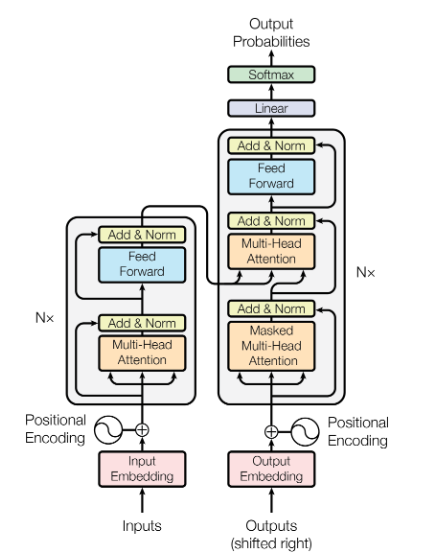
\includegraphics[width=.6\linewidth]{transformers.png}
        \caption{Архитектура модели класса Transformer}
        \label{transformer:image}
     \end{center}
\end{figure}

В контексте классификации текста модели класса Transformer могут использоваться для кодирования входного текста в векторное представление 
фиксированной длины, которое затем может быть передано в классификатор для прогнозирования метки класса. Обычно это делается с помощью 
предварительно обученной модели класса Transformer (такой как BERT или GPT) для кодирования текста, а затем добавления 
классификационного слоя и точной настройки модели на размеченном наборе данных с использованием подхода 
<<обучение с учителем>> (Supervised learning). 

\section{МОДЕЛИ}
Для исследования были выбраны следующие модели:
\begin{itemize}
    \item BERT;
    \item RoBERTa;
    \item DistilBERT;
    \item ALBERT;
    \item ELECTRA;
    \item OPT.
\end{itemize}

Это связано с тем, что эти архитектуры являются наиболее популярными при обработке естественного языка, в частности при классификации текстов, что связано с их эффективностью в этих задачах, а также небольшими затратами на обучение моделей данных архитектур. Для каждой архитектуры была взята модель базового размера. 
\subsection{BERT}
BERT (Bidirectional Encoder Representations from Transformers) является одной из самых популярных и используемых архитектур класса Transformer. BERT — это encoder-only (т.е. из transformer-блока encoder+decoder остаётся только encoder) двунаправленная модель, предобученная изначально на задачах размаскирования (Masked Language Modeling или MLM) и предсказания следующего предложения (Next Sentence Prediction или NSP).
Задача MLM заключается в следующем: 15\% токенов в исходной последовательности выбираются для возможной замены, 80\% заменяются токеном \texttt{[MASK]}, 10\% остаются без изменений, оставшиеся 10\% заменяются на случайный токен в словаре. В качестве целевого примера используется изначальная последовательность. Задача NSP ставится следующим образом: в качестве входной последовательности подаются два сегмента, разделённые специальным токеном \texttt{[SEP]}, а модель предсказывает, являются ли они последовательными сегментами из одного текста или нет. Обе задачи при обучении BERT решаются одновременно \cite{bert}.

\subsection{RoBERTa}
RoBERTa (Robustly optimized BERT approach) – версия модели BERT, для которой провели дополнительные исследования для улучшения качества итоговой модели. Результатами такого исследования стали следующие решения на этапе обучения модели:
\begin{itemize}
    \item Шаблон маскирования формируется динамически перед формированием набора примеров для одного шага оптимизации, тогда как в оригинальной модели шаблон маскирования формируется один раз перед обучением;
    \item Вместо сегментов текста подавались целиком предложения;
    \item Из итоговой функции потерь исключили добавку для задачи NSP, при этом данные формируются тем же образом (предложения подаются парами);
    \item Увеличили размер набора для одного шага оптимизации;
    \item Увеличили количество данных для обучения.
\end{itemize}
Такой подход позволил получить более эффективную модель на выходе \cite{roberta}.

\subsection{DistilBERT}
DistilBERT (Distilled BERT) — версия BERT, к которой применили процесс дистилляции знаний на фазе обучения, что позволило уменьшить размер модели на 40\%, сохранив при этом 97\% эффективности изначальной модели. Процесс заключается в том, чтобы сделать модель с меньшим количеством весов за счёт уменьшения количества слоёв относительно оригинальной модели в 2 раза, сохраняя ту же архитектуру, и при обучении сделать добавку в функцию ошибки, которая заставляет модель выдавать те же ответы, что и оригинальная модель. Обучалась модель на тех же данных и на той же задаче, что и BERT \cite{distilbert}.

\subsection{ALBERT}
ALBERT (A Lite BERT) –  ещё одна версия BERT, в архитектуру которой внесли изменения, позволяющие сократить количество параметров модели 
при сохранении её эффективности, что сокращает затраты на её обучения и использование. Для достижения этого эффекта были внесены следующие 
архитектурные изменения: 
\begin{enumerate}
    \item Добавлен дополнительный слой перед скрытыми, для того чтобы отделить размер входной последовательности от размера скрытого слоя;
    \item В разных слоях используются одни и те же веса, что позволяет уменьшить занимаемую моделью память при незначительном снижении качества модели.
\end{enumerate}
Помимо этого задачу NSP сменили на задачу предсказания порядка предложений (Sentence Order Prediction или SOP), что также улучшило качество итоговой модели. Задача SOP отличается от NSP подбором примеров: если в качестве негативных примеров в NSP брались сегменты из разных текстов, то в SOP в качестве негативных примеров используются последовательные сегменты текста, которые поменяли местами \cite{albert}.

\subsection{ELECTRA}
ELECTRA (Efficiently Learning an Encoder that Classifies Token Replacements Accurately) – модель, схожая в своей архитектуре с BERT. 
В отличие от оригинальной модели, обучение ELECTRA происходило следующим образом: есть две модели (Generator и Discriminator), которые обучаются вместе. 
Generator получает на вход последовательности с маскированными токенами и пытается их восстановить, 
а Descriminator пытается определить, какие токены в последовательности являются сгенерированными моделью-генератором, а какие изначально находились в последовательности. 
После обучения Generator не используется, а в Discriminator меняется выходной слой под нужную задачу, после чего дообучается уже на новой задаче. 
Такой метод обучения позволил уменьшить размеры модели, а соответственно и затраты на её обучение, при этом улучшив её эффективность
\cite{electra}.

\subsection{OPT}
OPT (Open Pre-trained Transformers) - это decoder-only модель, которая по сути является аналогом GPT-3 (Generative Pre-trained Transformers), 
но отличается от неё меньшими затратами на обучение и тем, что является полностью доступной, в отличие от GPT-3. Модель обучена на большом 
количестве данных изначально для генерации текста \cite{opt}.

\section{МЕТРИКИ}
Основными метриками для оценки моделей классификации являются accuracy (точность) и $F_1$. Изначально обе метрики вводятся для оценки качества 
решения задачи бинарной классификации, однако в задаче с большим количеством классов можно также использовать эти метрики: точность в том же виде,
а $F_1$ с некоторыми изменениями.

Accuracy показывает количество правильно данных моделью ответов и высчитывается по следующей формуле:
\begin{equation}
    \text{Accuracy} = \frac{K}{N},
\end{equation}
где:
\begin{itemize}
    \item $K$ -- количество правильно предсказанных примеров,
    \item $N$ -- общее количество примеров в выборке.
\end{itemize}
Однако такая метрика не является исчерпывающей, так как она не учитывает дисбаланс классов в выборке.

Более строгой и репрезентативной в данном случае является $F_1$-метрика. Она учитывает не только количество правильных ответов, но и 
ошибки первого и второго рода. В задаче бинарной классификации $F_1$ высчитывается по следующей формуле:
\begin{equation}
    F_1 = \frac{TP}{TP + \frac{FP + FN}{2}},
\end{equation}
где:
\begin{itemize}
    \item $TP$ -- количество правильно предсказанных меток первого класса,
    \item $FP$ -- количество неправильно предсказанных меток первого класса или ошибок первого рода (примеру второго класса присваивается метка первого класса),
    \item $FN$ -- количество неправильно предсказанных меток второго класса или ошибок второго рода (примеру первого класса присваивается метка второго класса).
\end{itemize}

Для задачи с большим количеством классов $F_1$ расширяется двумя способами:
\begin{enumerate}
    \item Macro $F_1$;
    \item Micro $F_1$.
\end{enumerate}

Macro $F_1$ высчитывается как среднее $F_1$ по каждому классу, а в micro $F_1$ составляющие $TP$, $FP$, $FN$ высчитываются как сумма 
соответствующих величин по каждому классу.  

	
\chapter{ОПИСАНИЕ РАЗРАБОТАННЫХ ПРОГРАММ}
	В качестве языка программирования для написания программ генерации данных и обучения моделей используется \texttt{Python}.
Для генерации данных использовались стандартные средства языка, а для их сохранения использовалась библиотека \texttt{Pandas}. Для использования и обучения моделей, для проведения экспериментов использовались специализированные библотеки: \texttt{Transformers}, \texttt{Datasets}, \texttt{WandB}, \texttt{Evaluate}.

\texttt{Transformers} используется для загрузки, хранения в облаке, использования и обучения моделей класса Transformer. Библиотека разработана 
HuggingFace и связана с открытым облачным хранилищем моделей HuggingFace. 

Ещё одной библиотекой от HuggingFace является \texttt{Datasets}. Эта библиотека используется для загрузки, хранения в облаке и использования 
наборов данных и связанных с ними метаданных. Кроме того, она связана с библиотекой \texttt{Transformers}, что позволяет быстро и просто 
использовать наборы данных из \texttt{Datasets} для обучения моделей с помощью \texttt{Transformers}.

Библиотека \texttt{Evaluate} так же разработана HuggingFace и используется для высчитывания различных метрик при обучении и тестировании моделей.

Библиотека \texttt{WandB} разработана Weights\&Biases. Используется для логирования процесса обучения, хранения моделей, наборов данных 
и визуализации метрик и других системных показателей во время обучения моделей. \texttt{WandB} также тесно связана с библиотекой 
\texttt{Transformers}. Кроме того, функционал библиотеки \texttt{WandB} позволяет дообучать несколько моделей с различными 
параметрами последовательно для проведении экспериментов, связанных с различными параметрами обучения моделей.

\section{ПРОГРАММА ДЛЯ ГЕНЕРАЦИИ ДАННЫХ}
В программе для создания набора данных были написана функция для создания примеров методом маскирования, которая принимает на вход список шаблонов, список сущностей для подстановки в шаблоны и маску, вместо которой подставляются сущности. Также была написана функция для перефразирования примеров с помощью соответсвущей модели, которая принимает на вход список примеров для перефразирования. Создание примеров вынесено в отдельные функции для каждого класса, после чего данные сохранялись в соответствущих файлах отдельно. Текст основных функций и пример генерации данных по одному из классов можно найти в приложении \ref{app:data-generating}.

\section{ПРОГРАММА ДЛЯ ПОИСКА ОПТИМАЛЬНЫХ ПАРАМЕТРОВ}
Для проведения исследования была разработана программа на языке \texttt{Python} с использованием описанных ранее библиотек. Программа 
загружает подготовленный набор данных и токенизирует его для дообучения модели. Далее с помощью функций класса из библиотеки \texttt{WandB} 
\texttt{sweep} обучается несколько моделей с различными параметрами обучения. Данные о процессе обучения и валидации во время обучения 
загружаются на сайт Weights\&Biases, и по ним автоматически строятся графики для анализа. Текст программы для исследования можно 
найти в приложении \ref{app:example}.

\section{ПРОГРАММА ДЛЯ СРАВНЕНИЯ МОДЕЛЕЙ}
Для сравнения моделей была разработана программа для обучения и тестирования моделей, а также логирования данных во время обучения 
с использованием описанных ранее библиотек. Программа состоит из 4-х блоков:
\begin{enumerate}
   \item Загрузка и предподготовка данных для обучения и тестирования;
   \item Загрузка модели для обучения и тестирования;
   \item Формирование параметров для обучения моделей;
   \item Обучение и тестирование.
\end{enumerate}

Данные о процессе обучения и валидации во время обучения загружаются на сайт Weights\&Biases и по ним автоматически строятся графики для анализа. Текст программы для исследования можно найти в приложении \ref{app:train}.

\chapter{НАБОР ДАННЫХ}
  \section{ВЫДЕЛЯЕМЫЕ ИНТЕНТЫ}
Прежде чем приступать к созданию набора данных, необходимо определить список намерений (интентов), которые система должна различать. 
При этом важно учитывать уровень взаимодействия игрока и неигровых персонажей (далее NPC): игрок может ожидать от NPC не только 
словесного ответа, но и каких-то действий, будь то торговля, обмен, перемещение NPC и т.д. 
Помимо этого, если игрок хочет просто поговорить, для формирования более корректного ответа важно понимать, что именно игрок говорит NPC: 
это приветствие, вопрос, касающийся знаний NPC о чём-то, и т.п.

Таким образом интенты можно разделить на две основные группы:
\begin{enumerate}
   \item Интенты для взаимодействия с игровой механикой;
   \item Интенты для более полного понимания диалога игрока с NPC.
\end{enumerate}
\subsection{Интенты для взаимодействия с игрой}
Перед составлением списка интентов, предполагающих взаимодействие с игрой, надо выделить универсальный для наибольшего количества игр
набор действий, которые может совершить NPC в ответ на реплику игрока. Проведя некоторое исследование, было решено выделить следующие действия:
\begin{itemize}
   \item Обмен или торговля (данные действия было решено не разделять, так как из реплики далеко не всегда может быть понятно, что именно хотел игрок);
   \item Нападение на других NPC;
   \item Перемещение NPC;
   \item Защита игрока, места или другого NPC;
   \item Передача устного сообщения;
   \item Следование за игроком или другим NPC;
   \item Стать напарником/помощником игрока;
   \item Передача предмета другому NPC;
   \item Выдача задания игроку;
   \item Завершение выполненного игроком задания;
   \item Реакция на угрозу от игрока (это может быть нападение NPC на игрока, паническое бегство или что-то ещё).
\end{itemize}
Каждому действию был присвоен соответствуюищй интент.
\subsection{Интенты для понимания фраз игрока в диалоге}
Для более корректной генерации ответа на фразу игрока были выделены следующие интенты:
\begin{itemize}
   \item Приветствие (для ответа на привествие со стороны игрока приветствием со стороны NPC);
   \item Вопрос, предполагающий наличие знаний NPC о других NPC или о мире игры в целом (для поиска контекста для модели генерации ответа в общей системе);
   \item Обычные фразы, не предполагающие наличие специальных знаний (например <<Что делаешь?>>, <<Как дела?>> и т.п.);
   \item Шутка (ответом на шутку может быть как смех, так и непонимание со стороны NPC);
   \item Бессмысленный набор букв или слов (ответ NPC предполагает непонимание фразы);
   \item Прощание (для ответа на прощание прощанием и передачи информации игре о завершении диалога).
\end{itemize}

\section{ГЕНЕРАЦИЯ ДАННЫХ}
Для получения основного корпуса данных был использован метод маскирования, часто использующийся для аугментации данных в задаче распознавания имён сущностей (Name Entity Recognition или NER). При использовании такого метода примеры в наборе данных получаются несколько однообразные, поэтому в дополнение к данным, полученным с помощью маскирования, добавляются данные, полученные с помощью модели перефразирования.

Так как метод маскирования позволяет сгенерировать очень большое количество примеров, было принято решение получить как можно больше таких данных, затем перемешать примеры, часть из них перефразировать с помощью модели, затем выбрать из перефразированных и изначальных примеров случайным образом некоторый набор данных в пропорции 1 к 1 (иногда из-за особенностей некоторых интентов пропорции смещались в ту или иную сторону). Таким образом, в итоговом наборе будут как более качественные примеры, полученные методом маскирования, так и менее качественные, полученные с помощью модели перефразирования.

Примеры для классификации бессмысленных запросов генерировались отдельно следующим образом: был создан набор слов и последовательностей 
символов, а из них случайным образом создавалась последовательность от 1 до 25 слов.

Важно заметить, что примеры для интента <<Шутка>> были взяты из открытых источников. Это связано с тем, что 
изменение шутки методом маскирования или перефразированием может исказить её смысл настолько, что шутка перестанет быть шуткой.

Ещё одним интентом, для которого данные не генерировались, является интент, обозначащий фразы игрока, 
не предполагающие наличие специальных знаний. Примеры для этого класса были взяты также из открытых источников, так как генерация таких 
примеров сложнее, а в открытых источниках имеются нужные данные.

\subsection{Метод маскирования}
Метод маскирования заключается в следующем: 
\begin{enumerate}
    \item Выбирается несколько примеров для аугментации;
    \item Выбранные сущности в них заменяются специальным набором символов, т.е. маской (например, \texttt{[ITEM]});
    \item Выбирается набор сущностей, которые могут находится в примерах на месте маски;
    \item В каждый пример вместо маски подставляются всевозможные варианты сущностей.
\end{enumerate}

Для генерации изначального набора примеров и сущностей была использована инструкционная модель от OpenAssistant. Кроме того, большое количество 
сущностей было получено переводом простых слов (яблоко, хлеб, меч, брюки, человек, торговец и т.п.) на английский язык.

Важно учитывать тот факт, что если подставлять вместо маски любые сущности или наборы сущностей, можно получить большое количество 
неадекватных примеров, например, <<Я хочу купить 2150 мечей>> и т.п. 

\subsection{Модель перефразирования}
В настоящее время существует множество сервисов для перефразирования текста, однако все или почти все из них либо являются платными, 
либо имеют  очень ограниченный бесплатный тарифный план, что не позволяет использовать их для перефразирования большого количества примеров. 
В связи с этим было принято решение использовать предобученную модель с HuggingFace. В качестве такой модели была выбрана модель 
\texttt{chatgpt\_paraphraser\_on\_T5\_base}. Это базовая модель T5, дообученная на датасете перефразирования, сгенерированном с помощью 
\texttt{ChatGPT}. Такой выбор связан с тем, что остальные модели, представленные на HuggingFace для этой задачи, оказались слишком слабыми: 
либо не меняли предложение, либо слишком сильно искажали изначальный смысл.

После проведения нескольких экспериментов был выбран наиболее удачный набор параметров (таблица \ref{tab1:table}).

\begin{table}[H]
   \captionsetup{format=hang, singlelinecheck=false}
   \raggedleft
      \caption{Параметры генерации для модели перефразирования}
      \label{tab1:table}
   \centering        
   \begin{tabular}{|p{10cm}|p{5cm}|}
      \hline
      num\_beams & 5 \\
      \hline
      num\_beams\_groups & 5 \\
      \hline
      num\_return\_sentences & 5 \\
      \hline
      repetition\_penalty & 10.0 \\
      \hline
      diversity\_penalty & 3.0 \\
      \hline
      no\_repeat\_ngram\_size & 2 \\
      \hline
      temperature & 0.7 \\
      \hline
      max\_length & 512 \\
      \hline
   \end{tabular}
\end{table}

\section{ОБРАБОТКА И АНАЛИЗ ПОЛУЧЕННЫХ ДАННЫХ}
В процессе генерации данных было обнаружено, что в некоторых ситуациях модель перефразирования текста может добавлять в примеры лишние символы, 
слова и целые фразы, что связано с датасетом, на котором она обучена. Например, модель может добавить ещё один или несколько дополнительных 
знаков препинания, кавычки, какую-то дополнительную информацию в скобках и т.п. Наличие таких ошибок в заметном количестве может сказаться на 
качестве итоговой модели, поэтому было решено избавиться от них.

Так как данные генерировались по классам, следующий этап предобработки заключается в объединении сгенерированных данных в единый набор и разделение на подвыборки для обучения, валидации и тестирования моделей. Для того, чтобы данные на разных подвыборках не сильно отличались друг от друга и в каждой подбвыборке распределение по классам было одинаковое, разделение происходило следующим образом:
\begin{enumerate}
   \item Данные по каждому классу загружались отдельно и перемешивались;
   \item Затем данные по каждому классу разделялись на разные подвыборки (8:1:1 на тренировку, валидацию и тестирование);
   \item После данные объединялись по подвыборкам и каждая из них перемешивалась. 
\end{enumerate}

После объединения был проведён анализ полученных данных. Общий размер набора данных примерно 2,2 миллиона токенов или 163,2 тысячи 
примеров. Средняя длина одного примера 13 токенов. 
В среднем количество примеров по каждому классу составляет около 10000 примеров (рисунок \ref{classnumbers:image}). 
Однако количество примеров по некоторым классам меньше 10000 (от 4000 до 7000), что связано со сложностью создания примеров для 
этих классов.
\begin{figure}[H]
   \begin{center}
      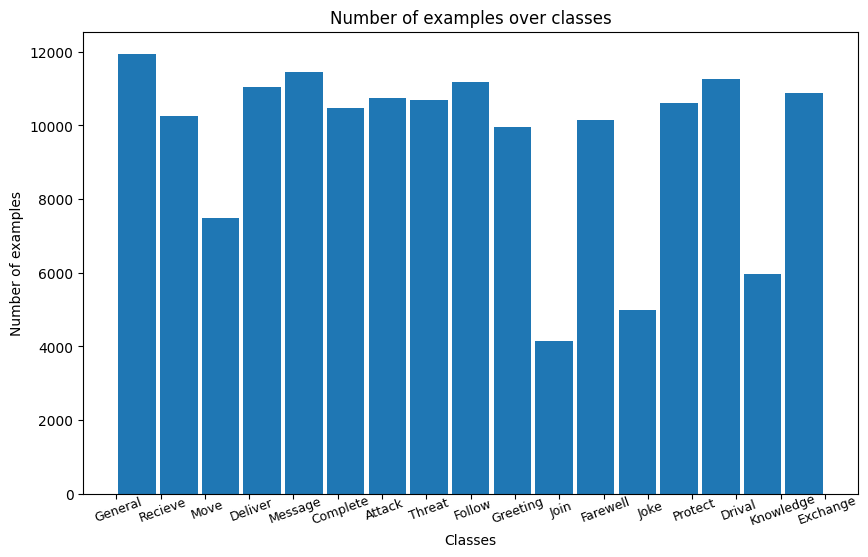
\includegraphics[width=.7\linewidth]{examples_over_classes.png}
      \caption{Распределение примеров по классам}
      \label{classnumbers:image}
   \end{center}
\end{figure}

Кроме того, набор имеет следующее распределение длин примеров в токенах (рисунок \ref{tokennumbers:image}).
\begin{figure}[H]
   \begin{center}
      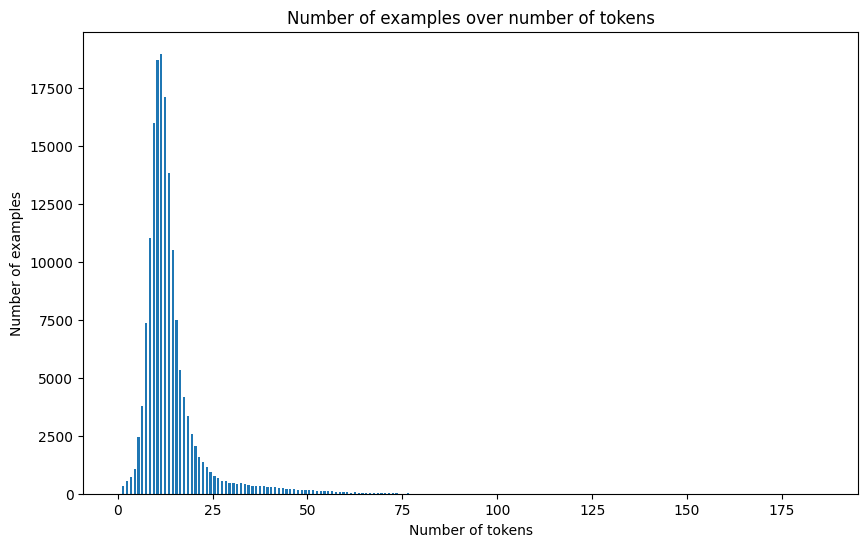
\includegraphics[width=.7\linewidth]{examples_over_tokens.png}
      \caption{Распределение примеров по количеству токенов}
      \label{tokennumbers:image}
   \end{center}
\end{figure}

Далее приведено несколько примеров из полученного набора данных (таблица \ref{examples:table}).
\begin{table}[H]
   \captionsetup{format=hang, singlelinecheck=false}
   \raggedleft
      \caption{Примеры из полученного набора данных}
      \label{examples:table}
   \centering        
   \begin{tabular}{|p{11cm}|p{5cm}|}
      \hline
      Примеры & Классы примеров \\
      \hline
      Your task is to hand saber to Annah. & Deliver \\
      \hline
      Hello, dear friends! & Greeting \\
      \hline
      tomorrow one integer hundred claim Follow elves drop man & Drival \\
      \hline
      Make sure you choose wisely, because every move counts, Beithira Soulforger! & Threat \\
      \hline
      I'd like to sell tomato, steak. & Exchange \\
      \hline
      I would like to buy pike and falchion. & Exchange \\
      \hline
      Could you come after Kieran Fireblood? & Follow \\
      \hline
      I want you to beat that bandit. & Attack \\
      \hline
      Are you capable of killing Annah? & Attack \\
      \hline
      You are responsible for safeguarding an outpost. & Protect \\
      \hline
      Please, go to this wayfarer. & Move \\
      \hline
      What can you tell me about Caravan Crossroads? & Knowledge \\
      \hline
      We will never speak again, Adira Whitesnow. & Farewell \\
      \hline
      Please take care Brianna Moonlight. & Farewell \\
      \hline
      Join me. & Join \\
      \hline
      i don't know. & General \\
      \hline
      Why does lightning always strike trees? They are the path of leaf resistance. & Joke \\
      \hline
      Can i find mission for me in Goldgrasp? & Recieve quest \\
      \hline
      May I ask you to communicate with Hargrimm the Bleak. & Message \\
      \hline
      I've completed your job in Deeproot Village. & Complete quest \\
      \hline
   \end{tabular}
\end{table}

\chapter{ВЫБОР ОПТИМАЛЬНЫХ ПАРАМЕТРОВ ОБУЧЕНИЯ}
  \section{ТЕХНОЛОГИЯ ИССЛЕДОВАНИЯ}
Чтобы сравнение моделей между собой было более корректным, важно подобрать оптимальные параметры для дообучения каждой модели. Основными параметрами, влияющими на дообучение моделей являются learning rate (темп обучения), learning rate scheduler (изменение learning rate в процессе обучения) и weight decay (сокращение весов или $L_2$ регуляризация). Каждая модель дообучается несколько раз с различными параметрами, после чего для каждой из них выбирается наиболее оптимальный набор параметров. В качестве основной метрики для выбора лучших параметров дообучения использовалась accuracy (точность), так как в процессе анализа графиков метрик во время обучения было замечено, что micro $F_1$ и macro $F_1$ не сильно отличаются от accuracy (не более 1\%).

Все модели дообучались на 8 эпохах с ранней остановкой. Условие для ранней остановки: функция ошибки на валидационных данных не уменьшается в течение 3-х эпох.

\section{РЕЗУЛЬТАТЫ ИССЛЕДОВАНИЯ}
Для анализа и выбора оптимальных параметров будем использовать графики точности на валидационных данных в процессе обучения. На каждом рисунке 
представлены графики точности на валидационных данных во время обучения по одной модели с разными параметрами. Остальные графики (функция ошибки 
при обучении, функция ошибки на валидационных данных, micro $F_1$, macro $F_1$) можно найти в приложении \ref{app:sweeps}.
\subsection{BERT}
По графику точности, полученному в результате серии экспериментов (рисунок \ref{bert-accuracy:image}), можно сделать вывод, что наиболее 
оптимальными для дообучения BERT являются следующие параметры:
\begin{itemize}
    \item learning rate: 1,3e-4;
    \item learning rate scheduler: constant;
    \item weight decay: 7e-2.
\end{itemize}

\begin{figure}[H]
    \begin{center}
       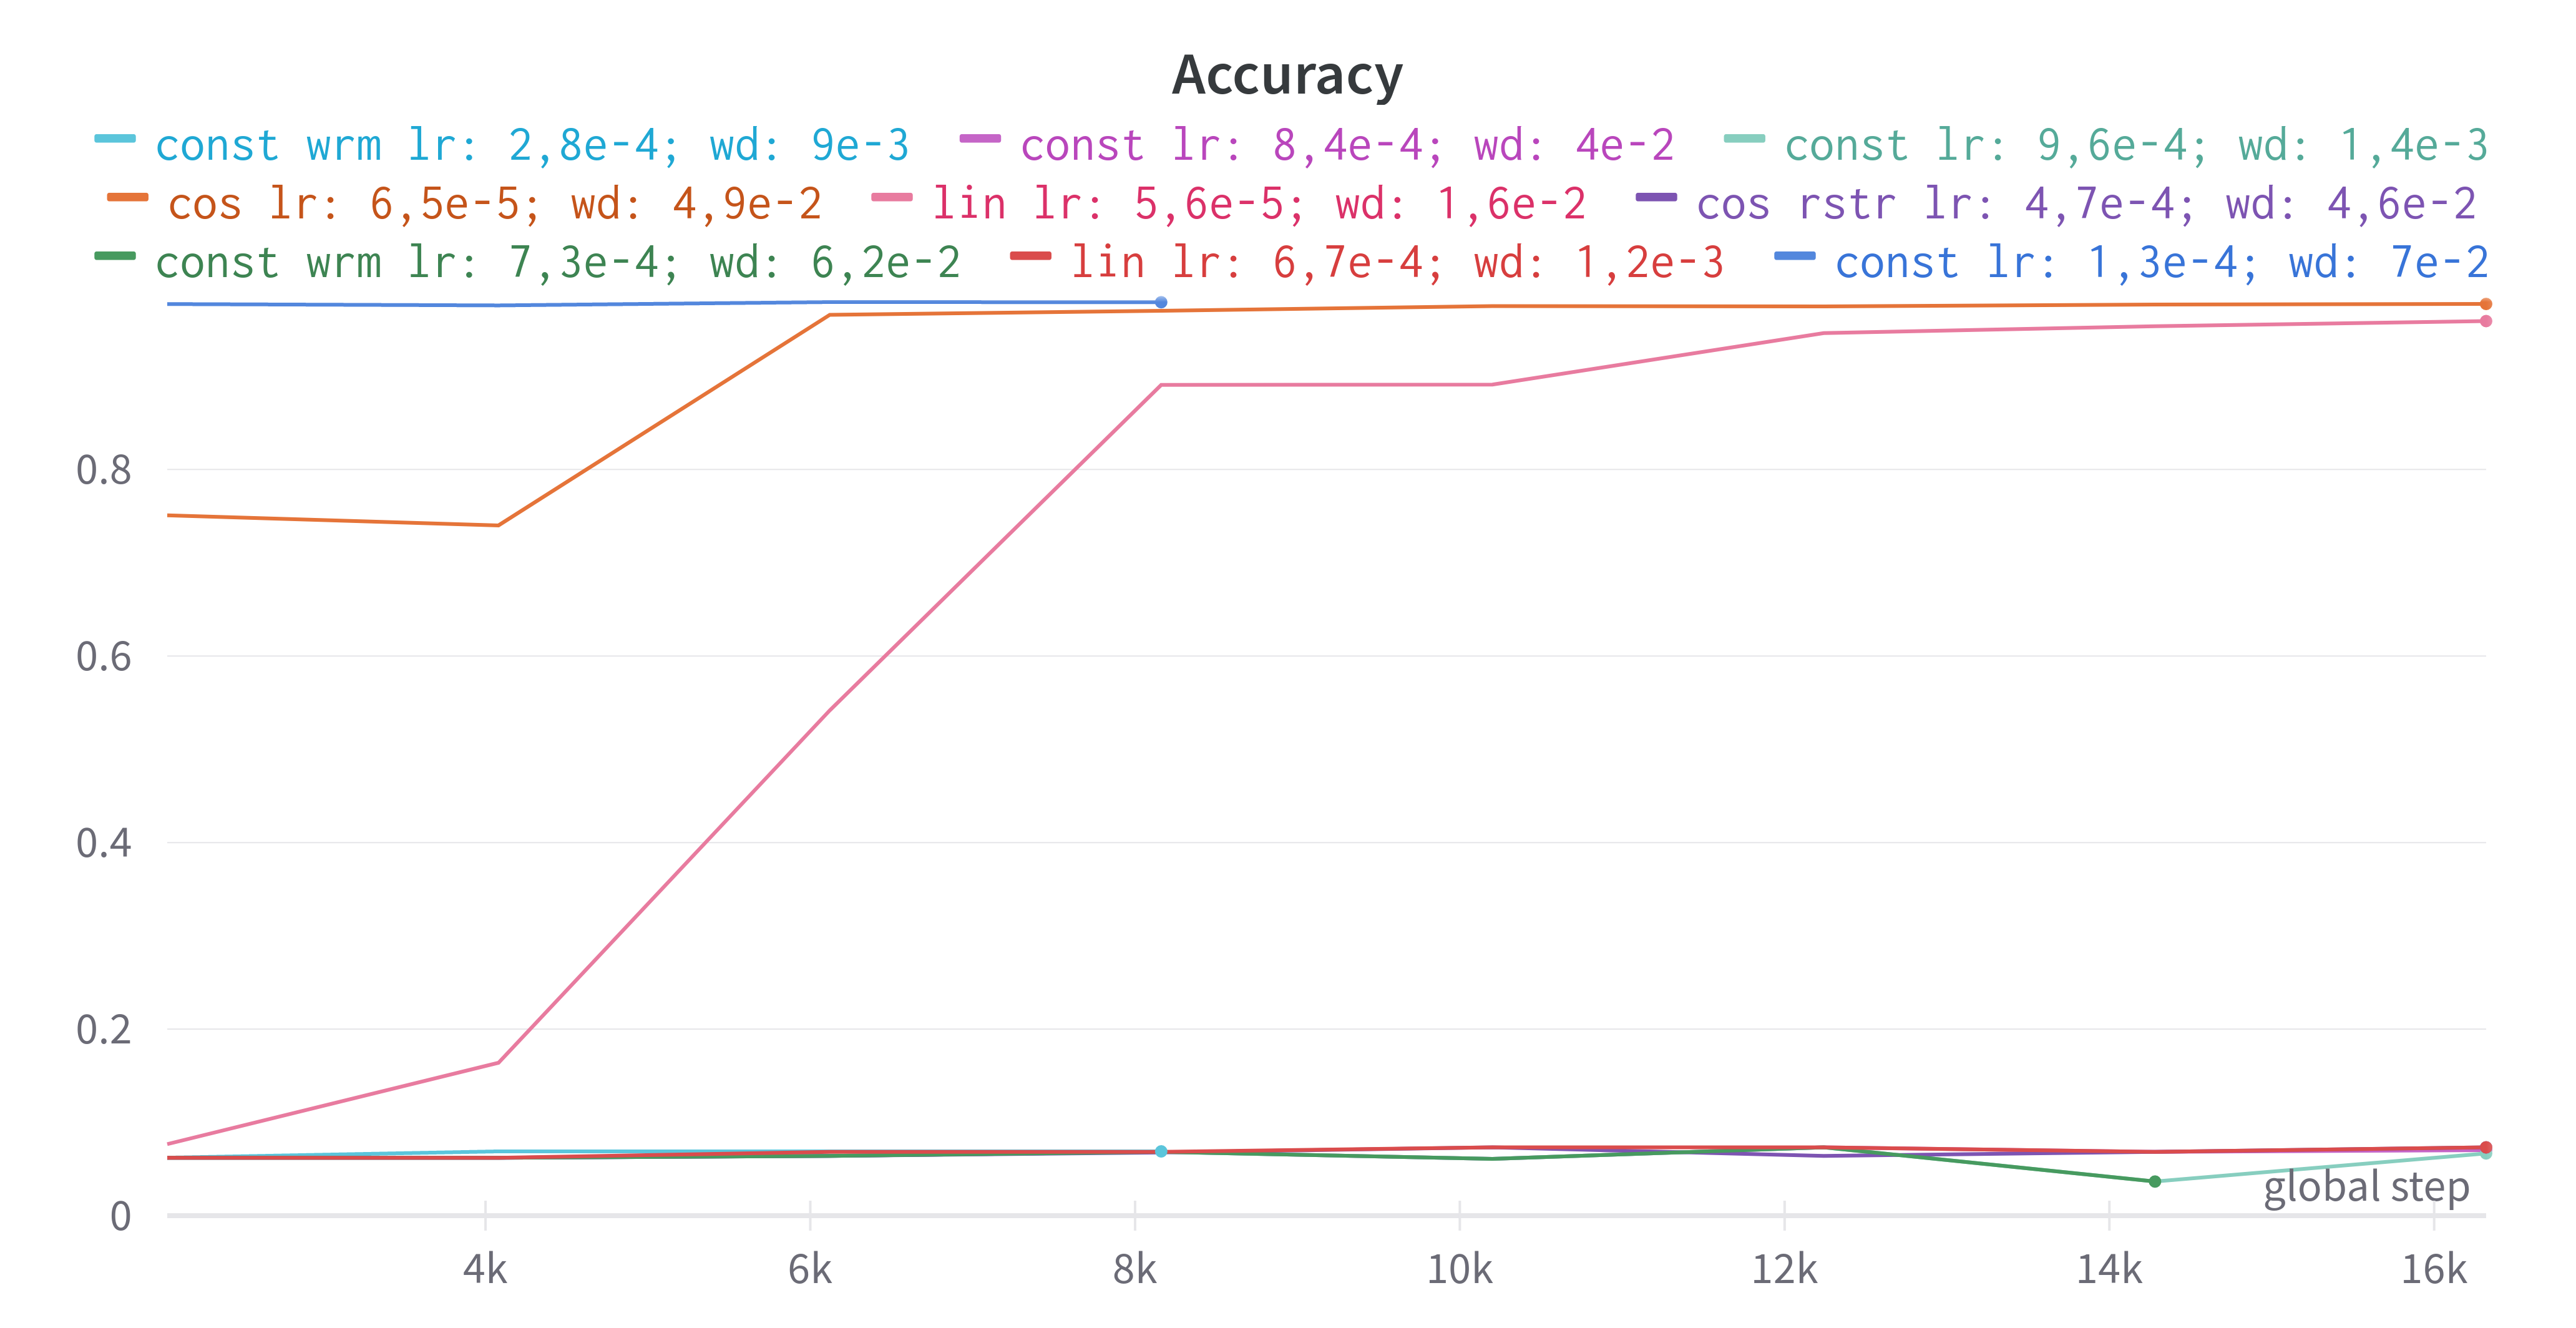
\includegraphics[width=.8\linewidth]{bert/accuracy.png}
       \caption{График точности во время обучения BERT}
       \label{bert-accuracy:image}
    \end{center}
\end{figure}
\subsection{RoBERTa}
После дообучения серии моделей по графику точности во время обучения (рисунок \ref{roberta-accuracy:image}) можно сделать вывод, 
что оптимальными для обучения RoBERTa на текущей задаче являются параметры:
\begin{itemize}
    \item learning rate: 5e-5;
    \item learning rate scheduler: linear;
    \item wight decay: 0.
\end{itemize}
\begin{figure}[H]
    \begin{center}
       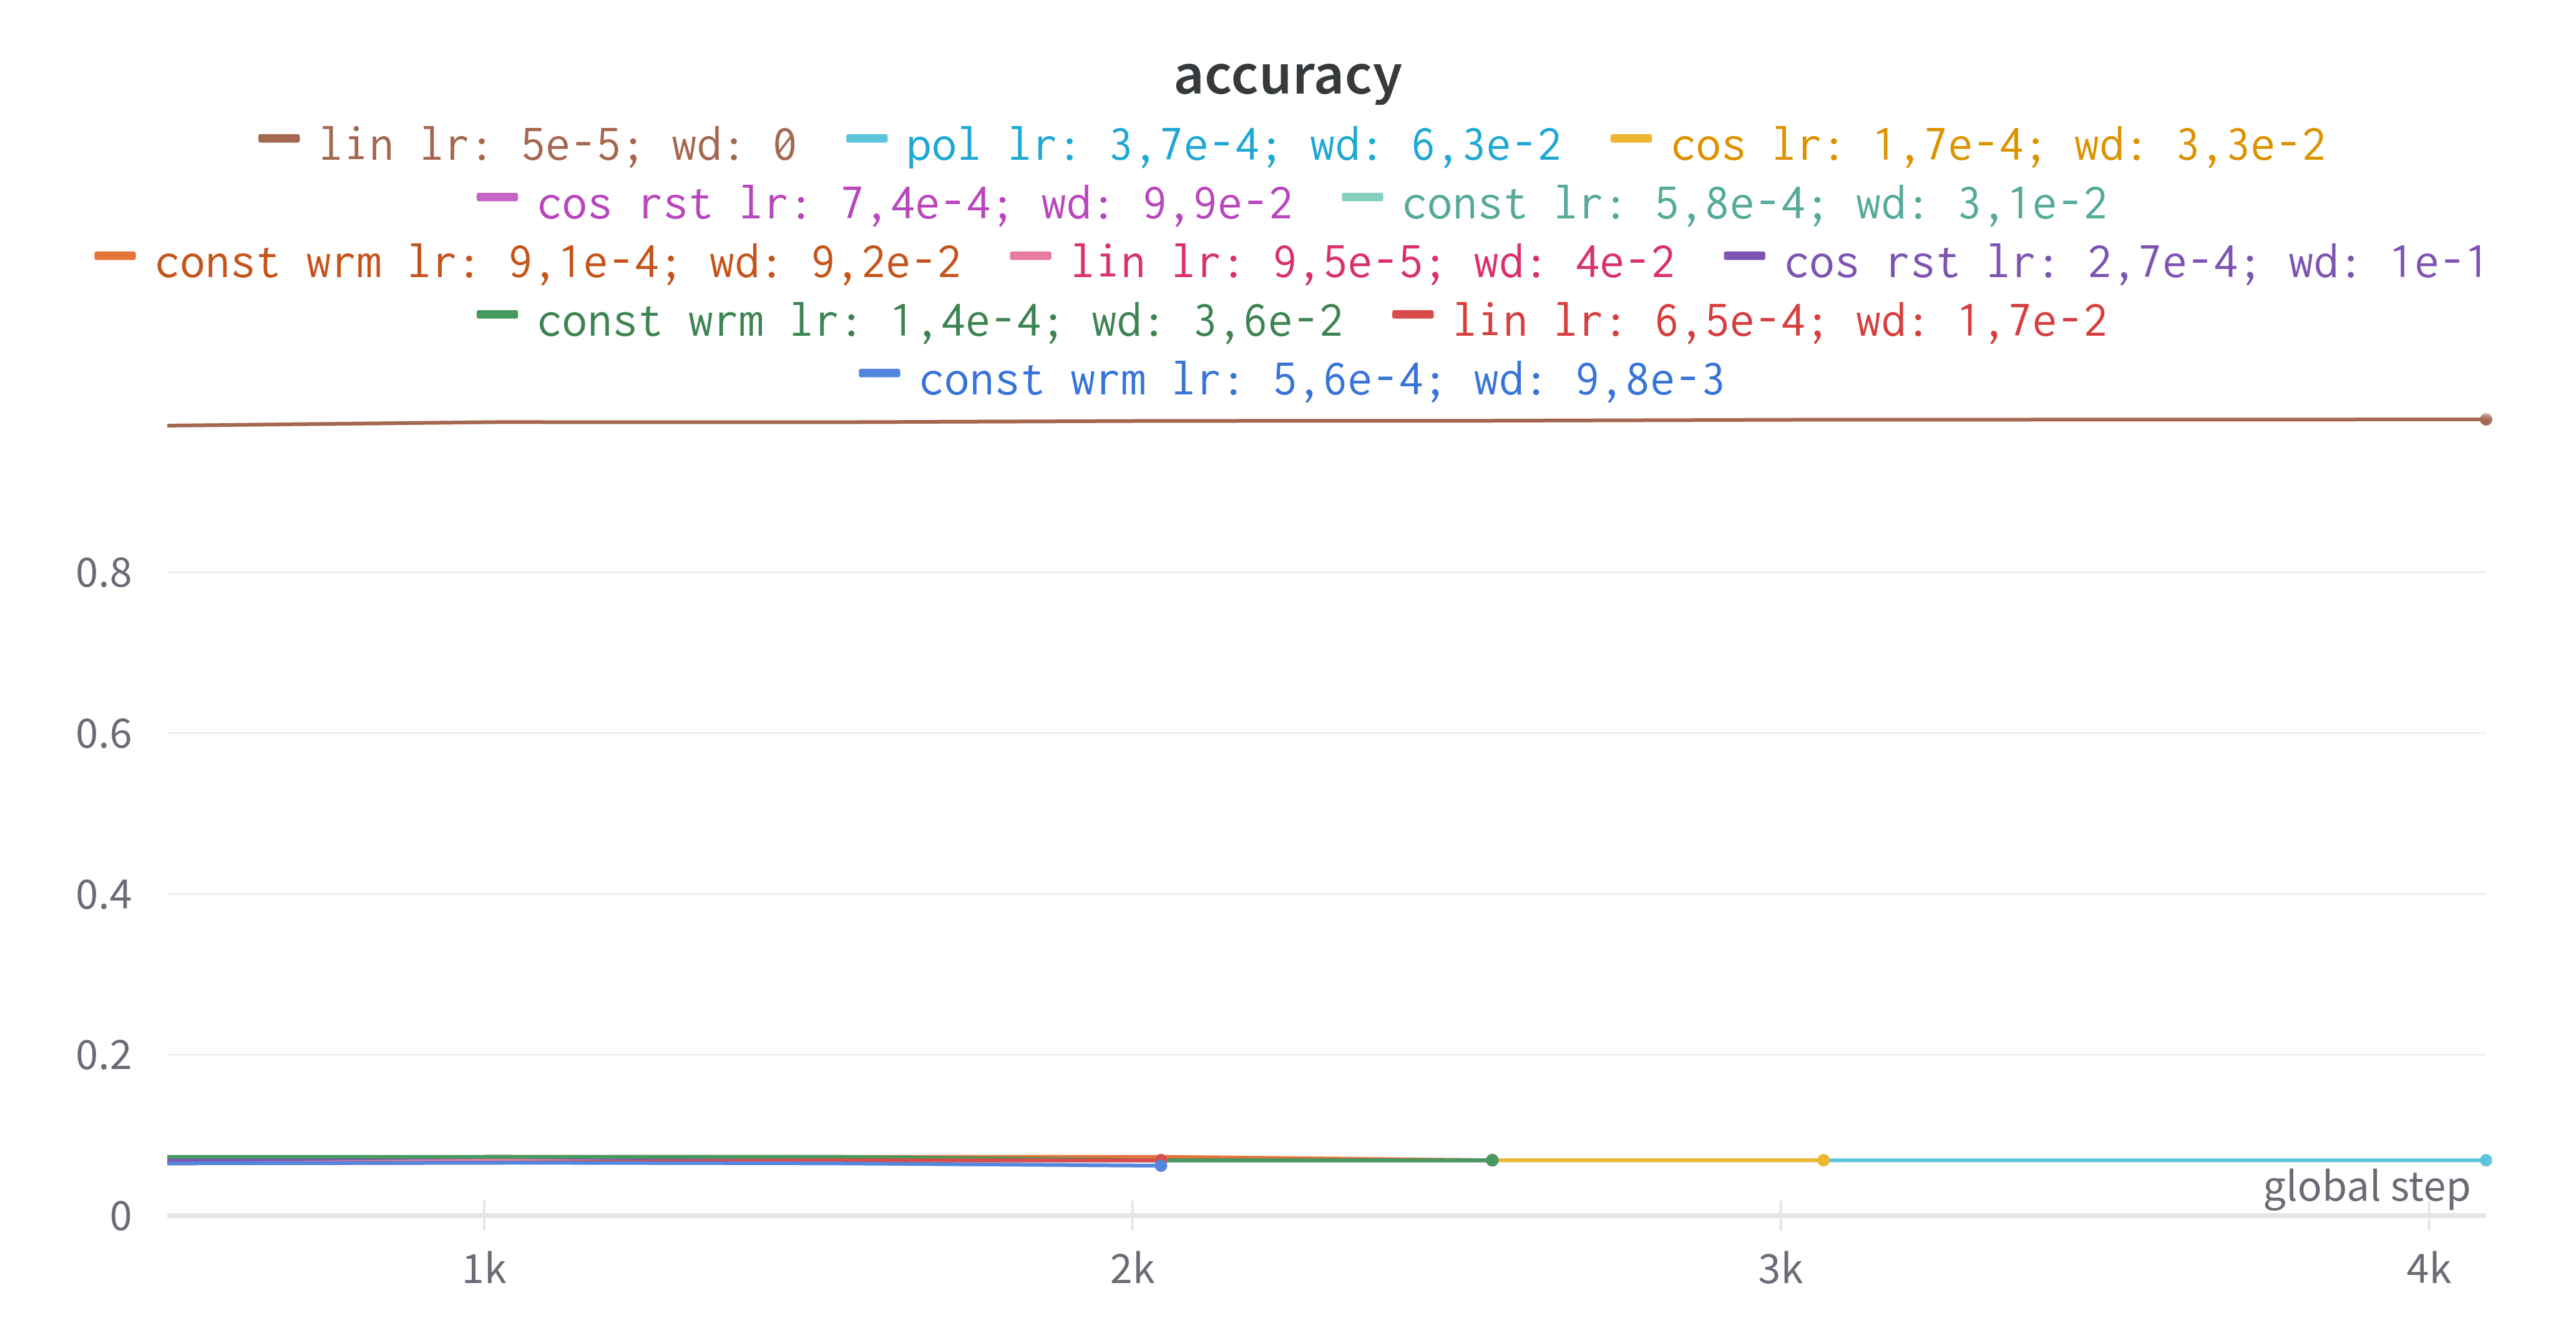
\includegraphics[width=.8\linewidth]{roberta/accuracy.png}
       \caption{График точности во время обучения RoBERTa}
       \label{roberta-accuracy:image}
    \end{center}
\end{figure}

\subsection{DistilBERT}
По графику точности во время обучения моделей (рисунок \ref{distilbert-accuracy:image}) об оптимальных параметрах обучения DistilBERT
можно сделать следующий вывод:
\begin{itemize}
    \item learning rate: 1,8e-4;
    \item learning rate scheduler: linear;
    \item weight decay: 0.
\end{itemize}
\begin{figure}[H]
    \begin{center}
       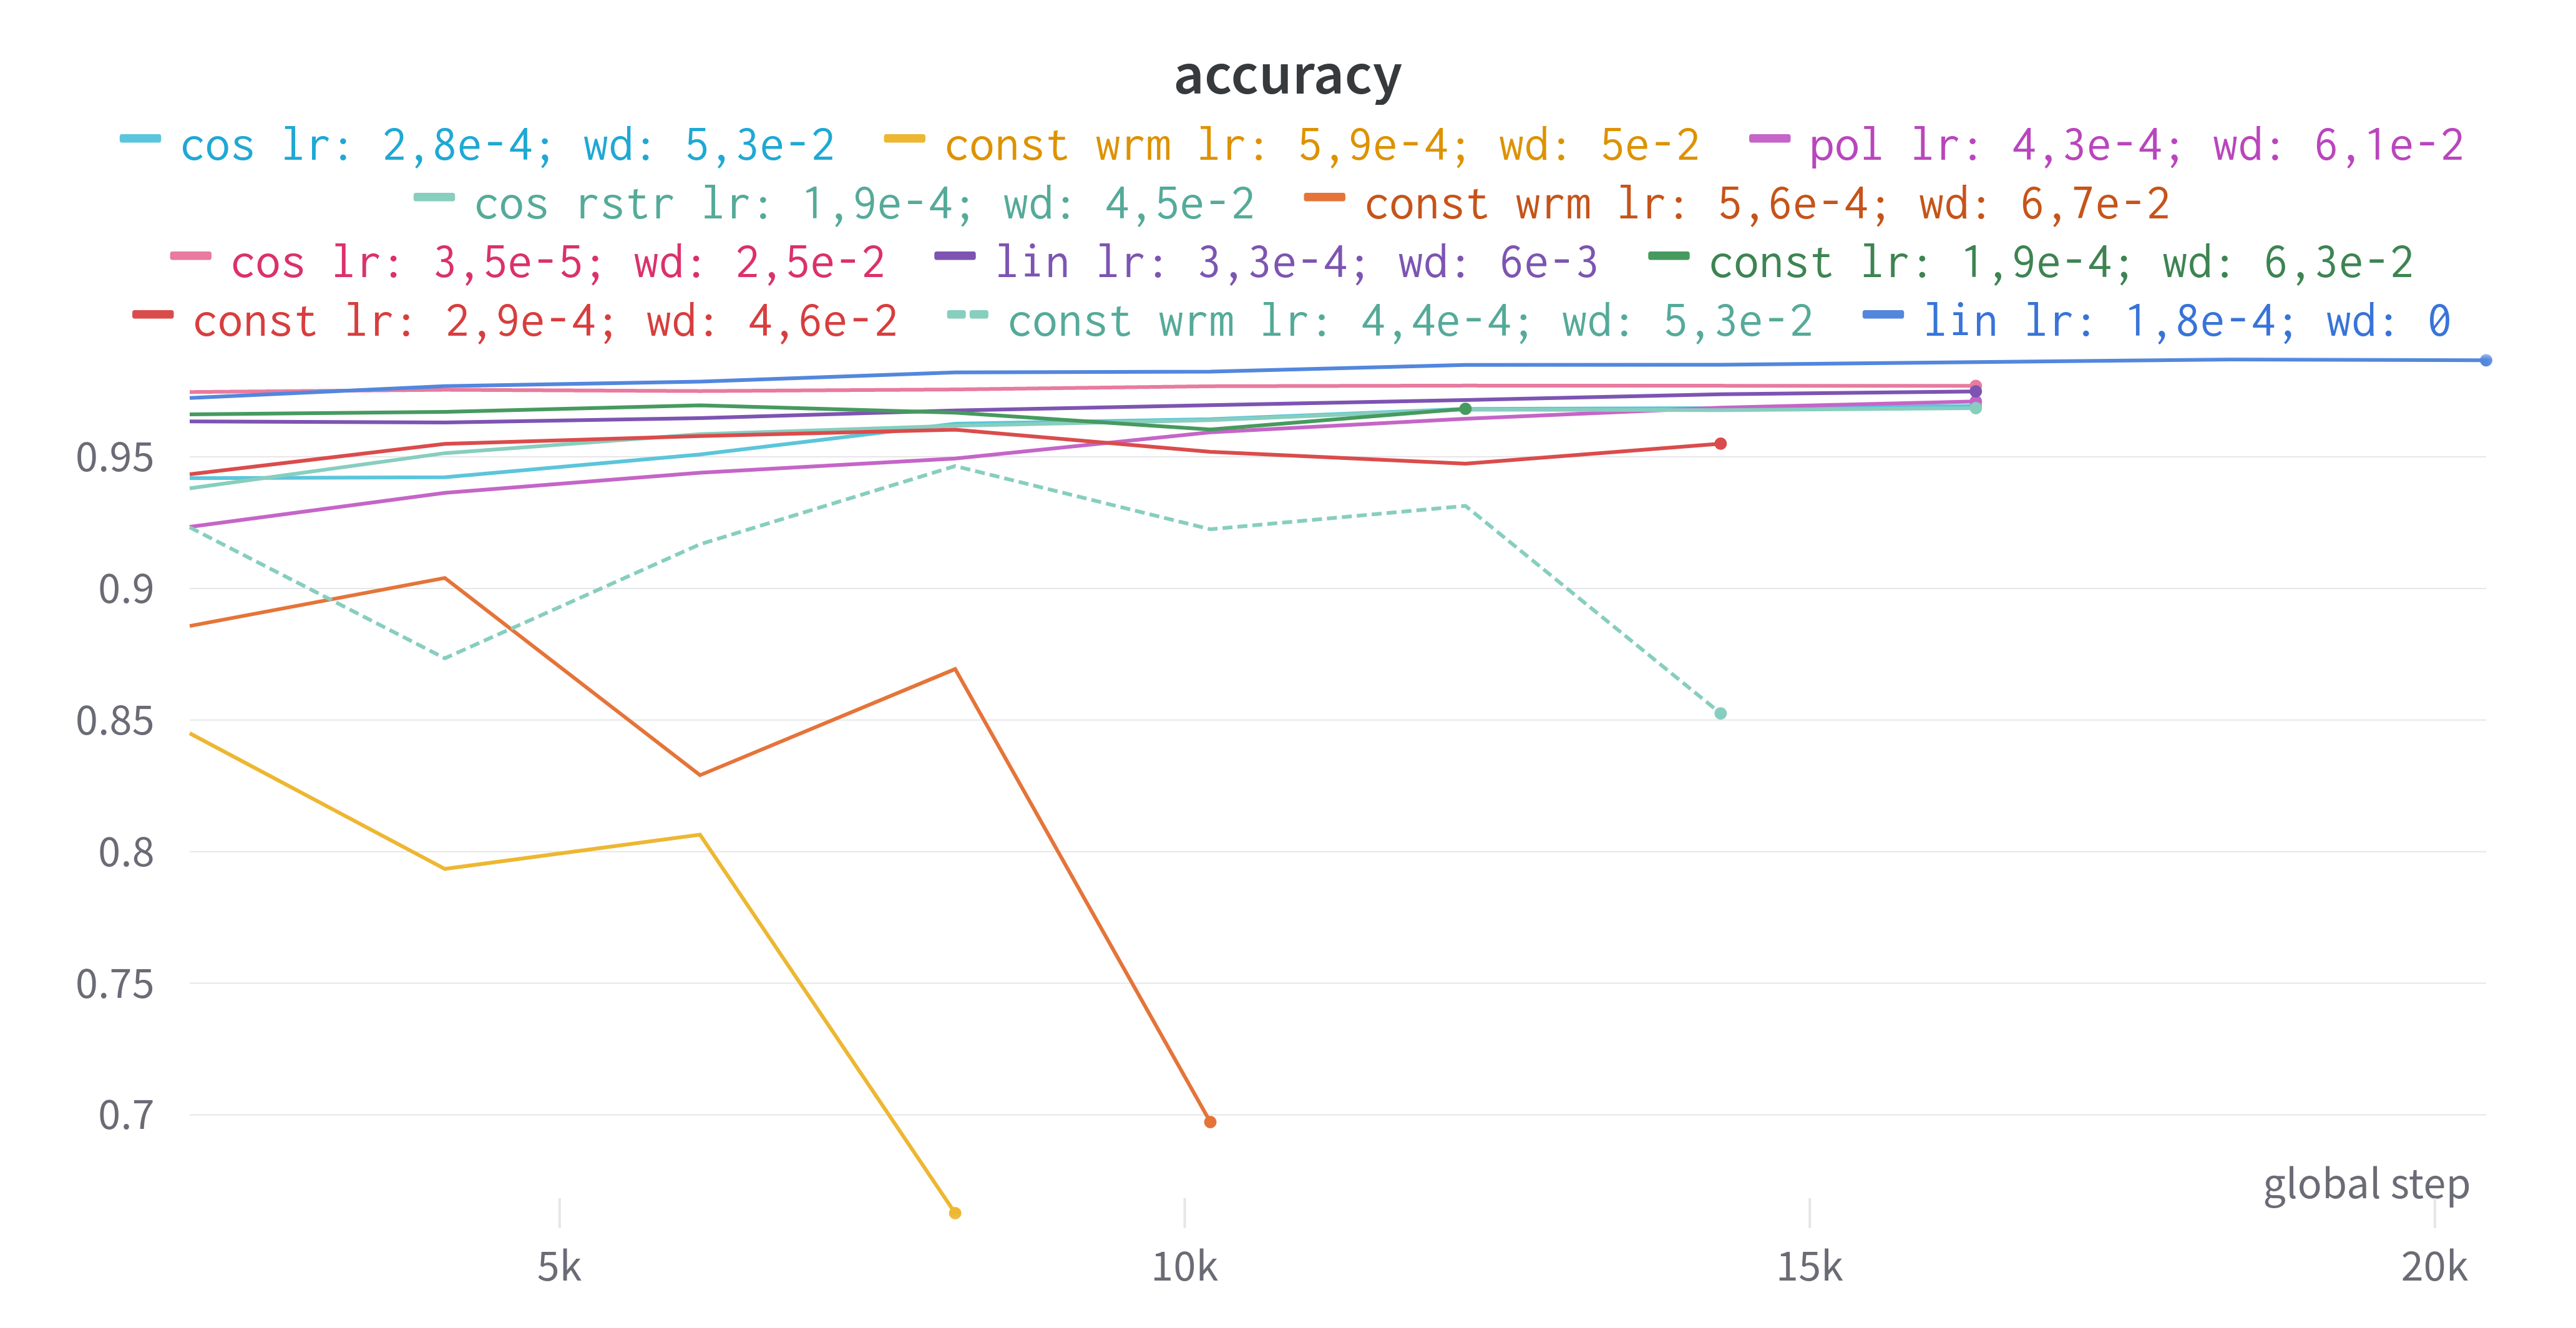
\includegraphics[width=.8\linewidth]{distilbert/accuracy.png}
       \caption{График точности во время обучения DistilBERT}
       \label{distilbert-accuracy:image}
    \end{center}
\end{figure}

\subsection{ALBERT}
Проведя анализ графика точности во время обучения моделей (рисунок \ref{albert-accuracy:image}), оптимальные параметры дообучения ALBERT были определены следующим образом:
\begin{itemize}
    \item learning rate: 5e-5;
    \item learning rate scheduler: linear;
    \item weight decay: 0.
\end{itemize}
\begin{figure}[H]
    \begin{center}
       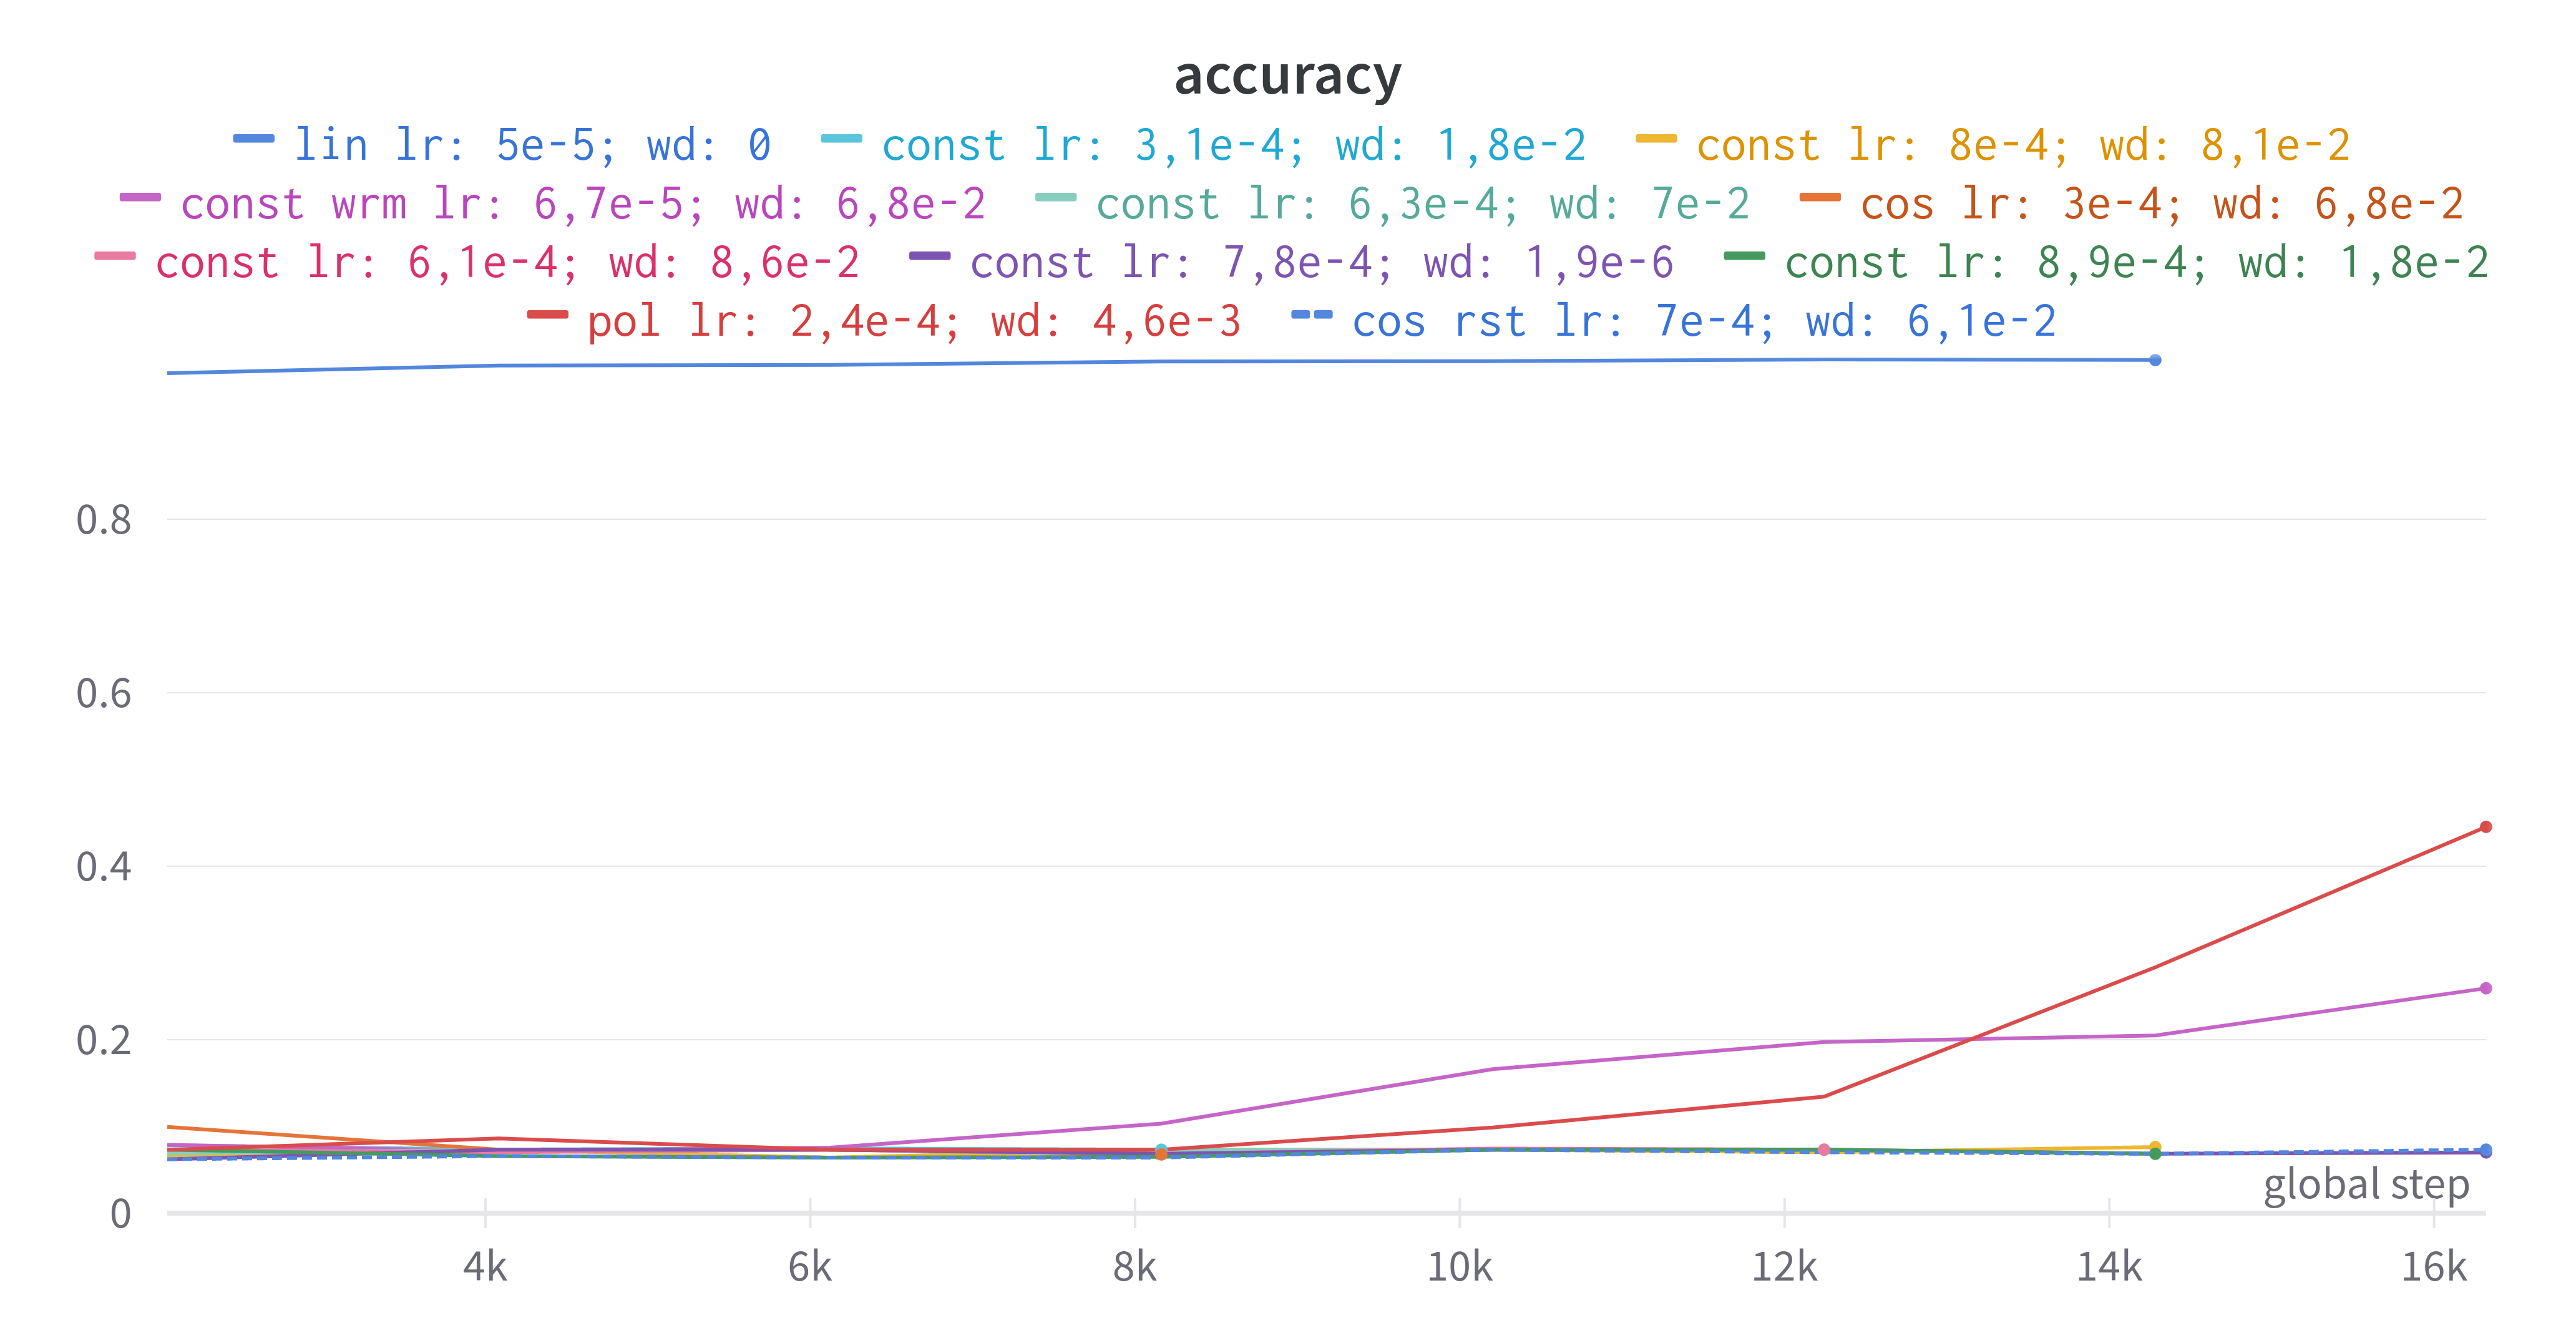
\includegraphics[width=.8\linewidth]{albert/accuracy.png}
       \caption{График точности во время обучения ALBERT}
       \label{albert-accuracy:image}
    \end{center}
\end{figure}

\subsection{ELECTRA}
После проведения серии экспериментов по графику точности во время обучения моделей (рисунок \ref{electra-accuracy:image}) можно выбрать следующие 
оптимальные для дообучения ELECTRA параметры:
\begin{itemize}
    \item learning rate: 6,6e-5;
    \item learning rate scheduler: cosine with restarts;
    \item weight decay: 4,8e-3.
\end{itemize}
\begin{figure}[H]
    \begin{center}
       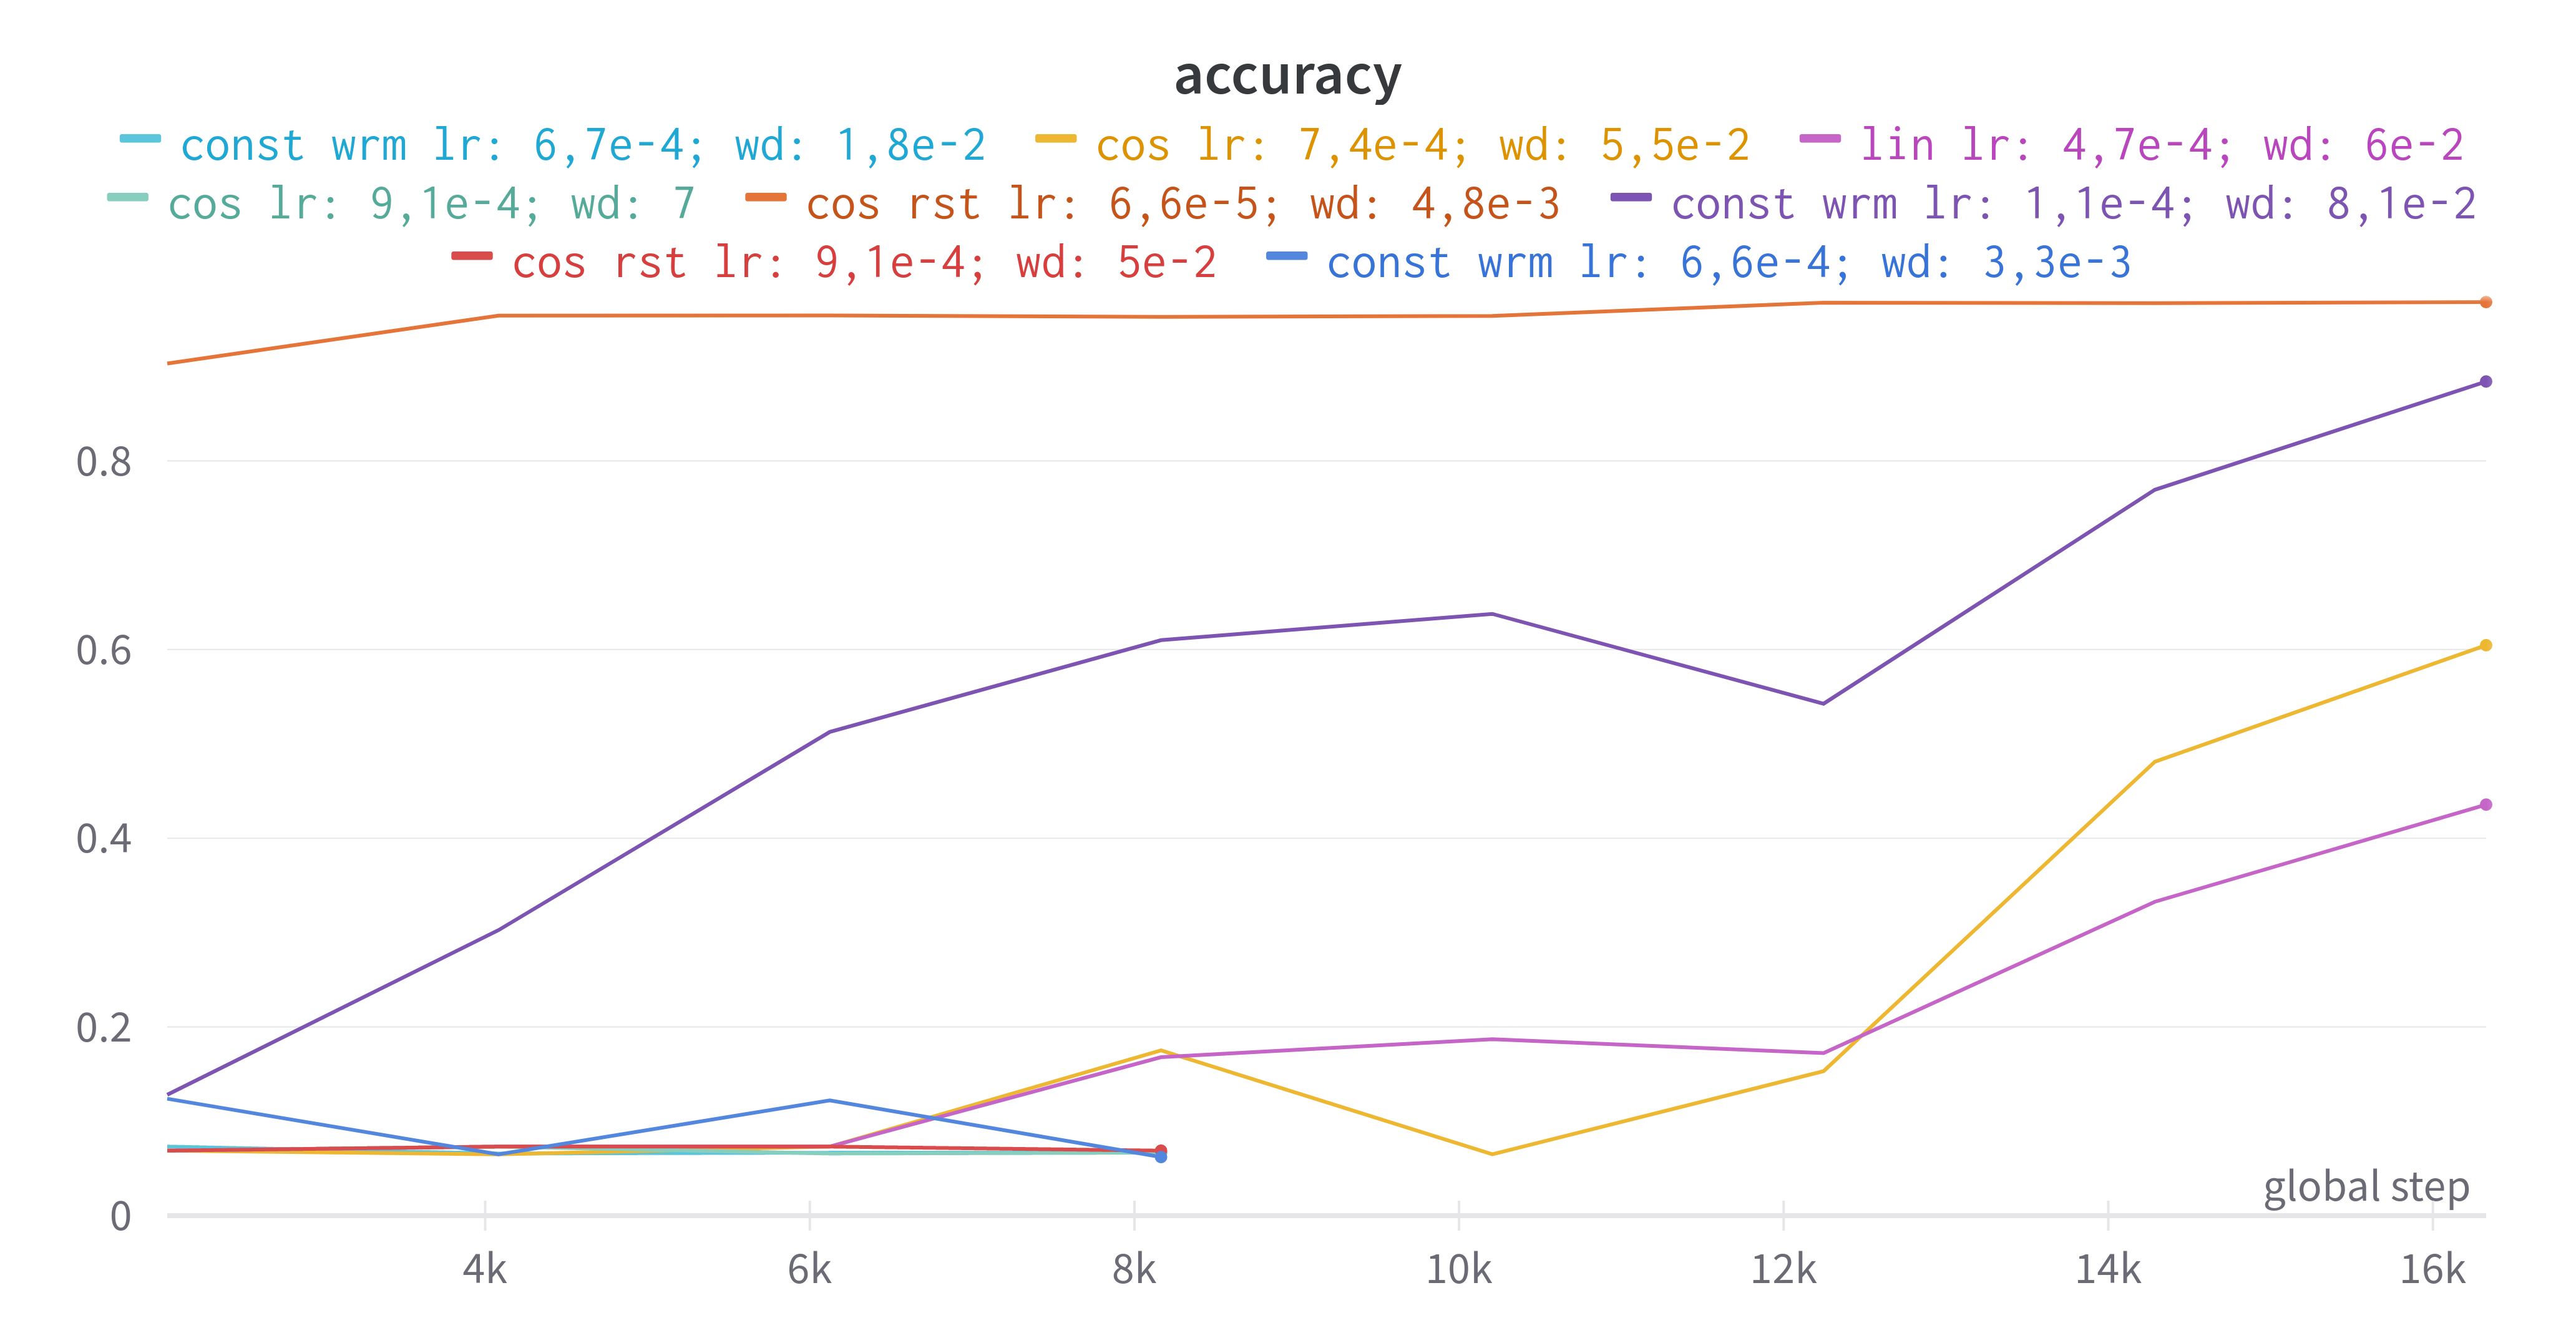
\includegraphics[width=.8\linewidth]{electra/accuracy.png}
       \caption{График точности во время обучения ELECTRA}
       \label{electra-accuracy:image}
    \end{center}
\end{figure}

\subsection{OPT}
По графику точности во время обучения моделей (рисунок \ref{opt-accuracy:image}) об оптимальности параметров дообучения OPT можно сделать 
следующий вывод:
\begin{itemize}
    \item learning rate: 5e-5;
    \item learning rate scheduler: linear;
    \item weight decay: 0.
\end{itemize}
\begin{figure}[H]
    \begin{center}
       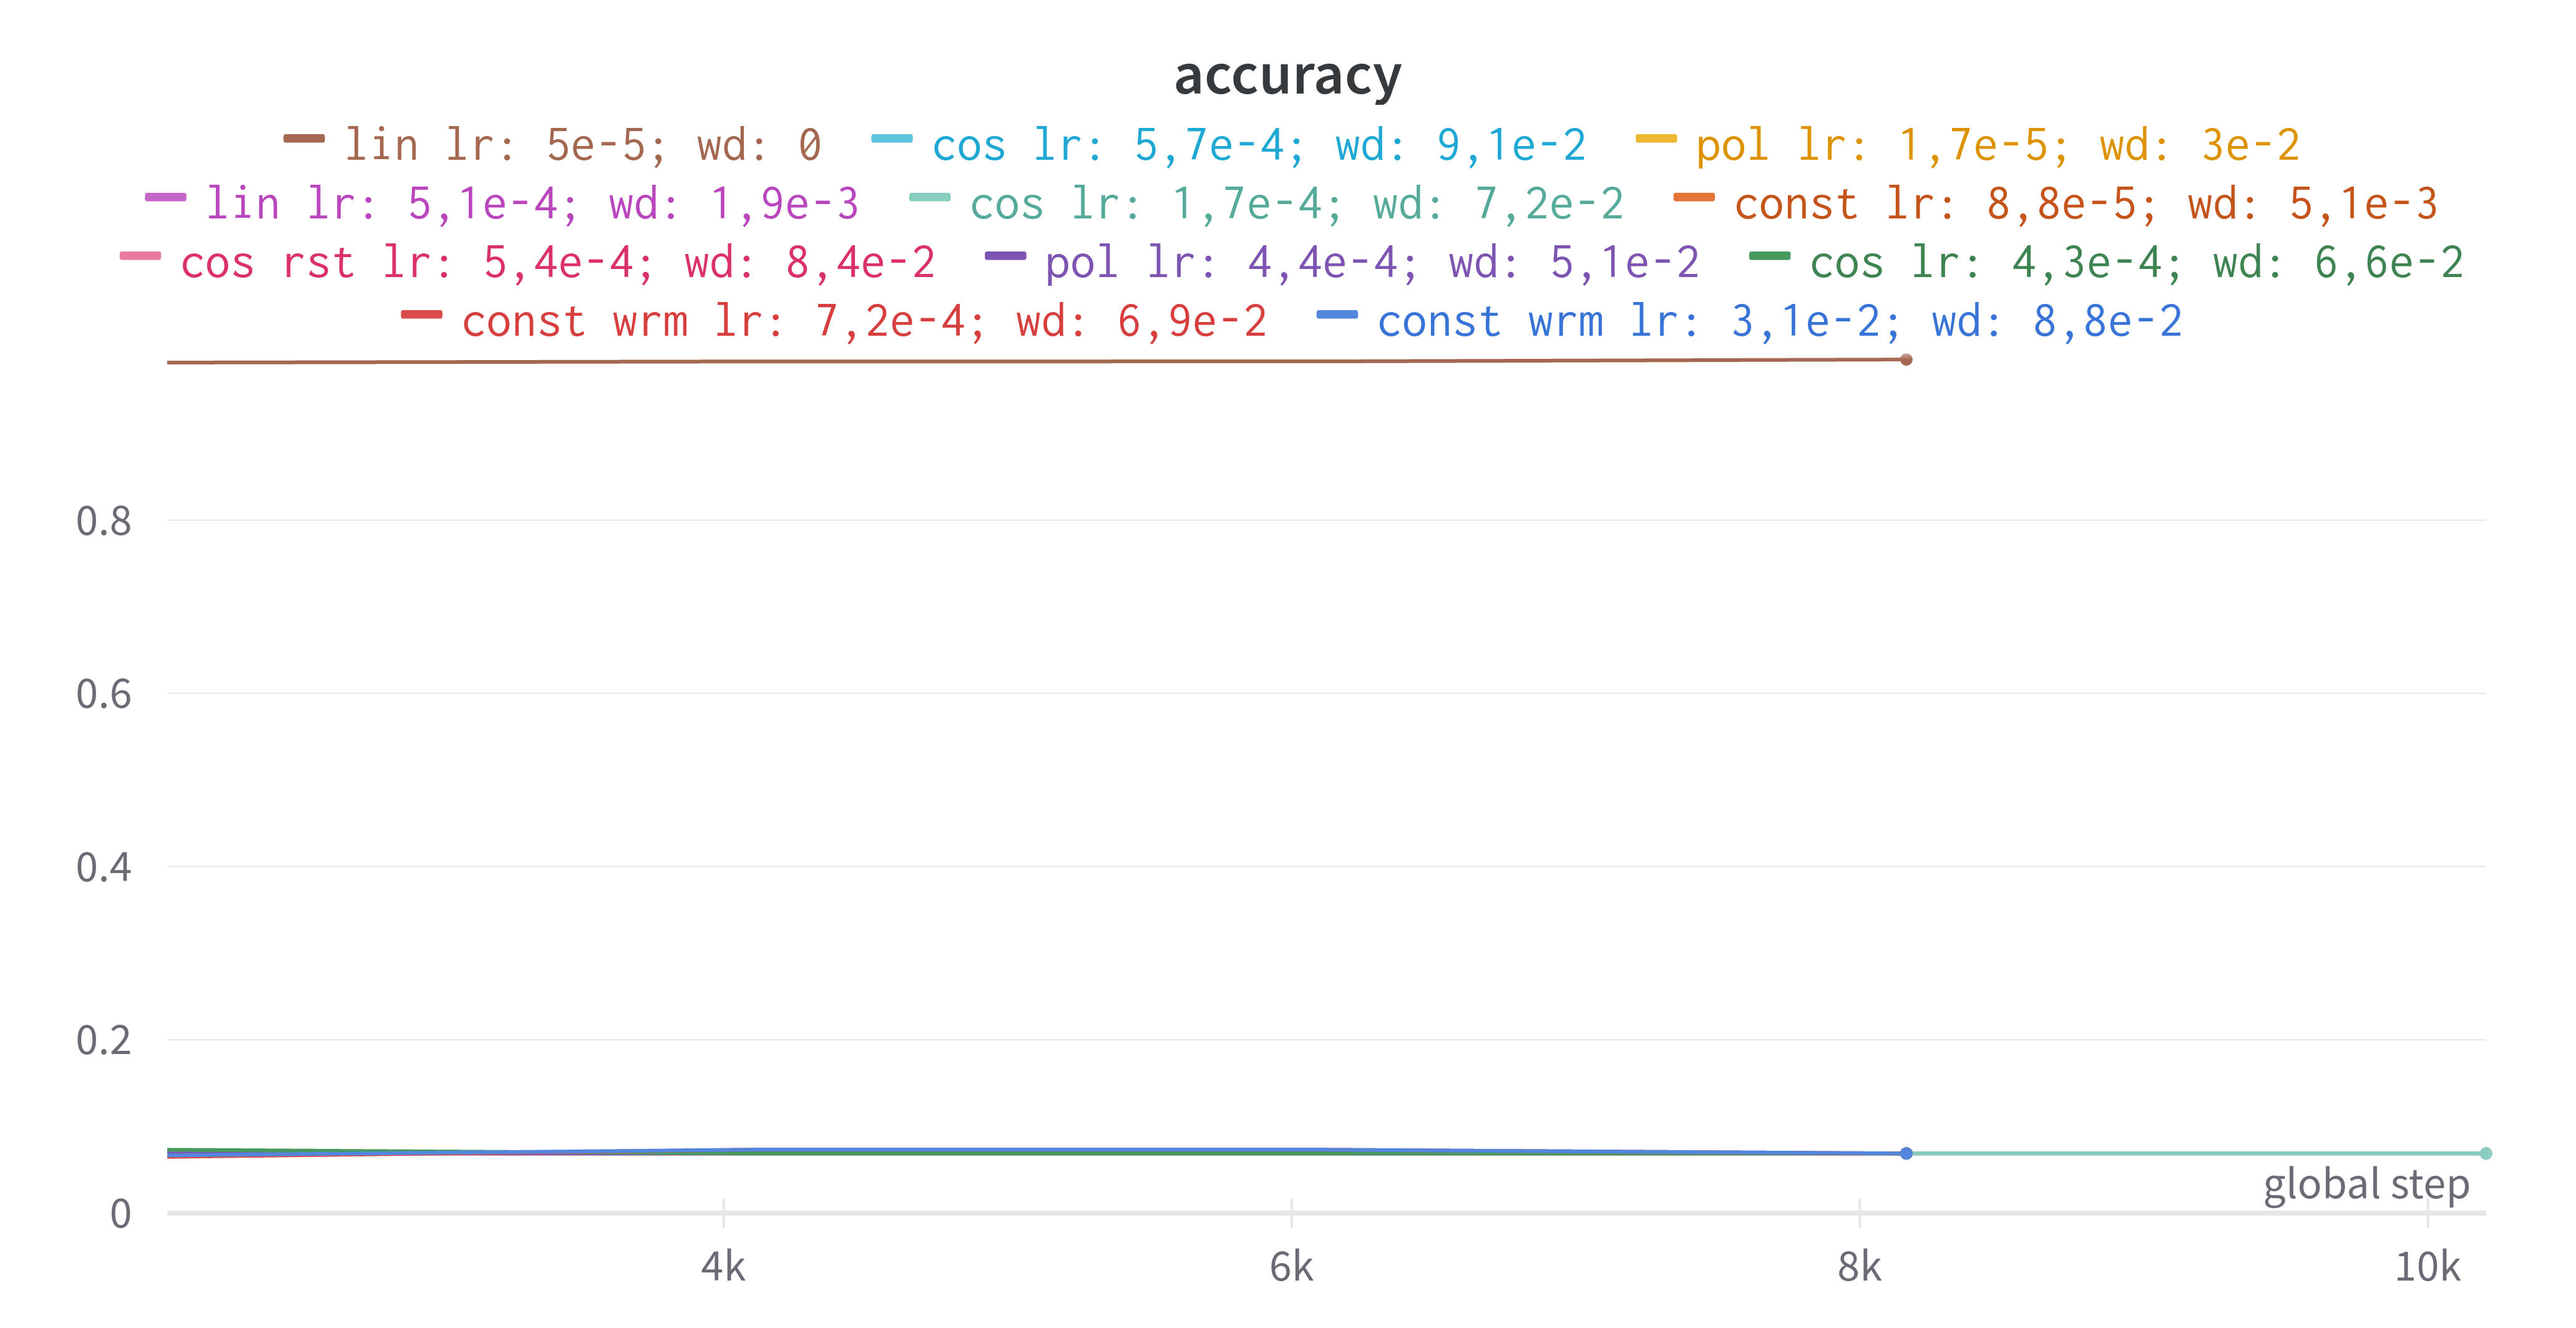
\includegraphics[width=.8\linewidth]{opt/accuracy.png}
       \caption{График точности во время обучения OPT}
       \label{opt-accuracy:image}
    \end{center}
\end{figure}

\chapter{СРАВНЕНИЕ МОДЕЛЕЙ}
  \section{ТЕХНОЛОГИЯ ИССЛЕДОВАНИЯ}
На текущем этапе каждая из моделей дообучалась с оптимальными параметрами, а затем тестировалась. В качестве основных метрик для сравнения использовались accuracy, micro $F_1$ и macro $F_1$ на валидационных данных во время обучения. Кроме того, для выбора наиболее эффективной модели важно учитывать также данные о времени обучения, количестве занимаемой памяти во время обучения и количестве операций с плавающей точкой, затраченных на обучение моделей, а также скорость во время тестирования.

Все модели дообучались на 8 эпохах с ранней остановкой. Условие для ранней остановки: 
функция ошибки на валидационных данных не уменьшается в течение 3-х эпох.
\section{РЕЗУЛЬТАТЫ ИССЛЕДОВАНИЯ}
Проведя анализ графиков метрик во время обучения моделей 
(рисунок \ref{models-accuracy:image}, рисунок \ref{f1-macro:image}, рисунок \ref{f1-micro:image}) можно сделать вывод, что наиболее точной 
моделью является RoBERTa, тогда как наименее точной моделью оказался BERT. Однако стоит отметить, что точность моделей отличается незначительно 
(около 1\%). 
\begin{figure}[H]
   \begin{center}
      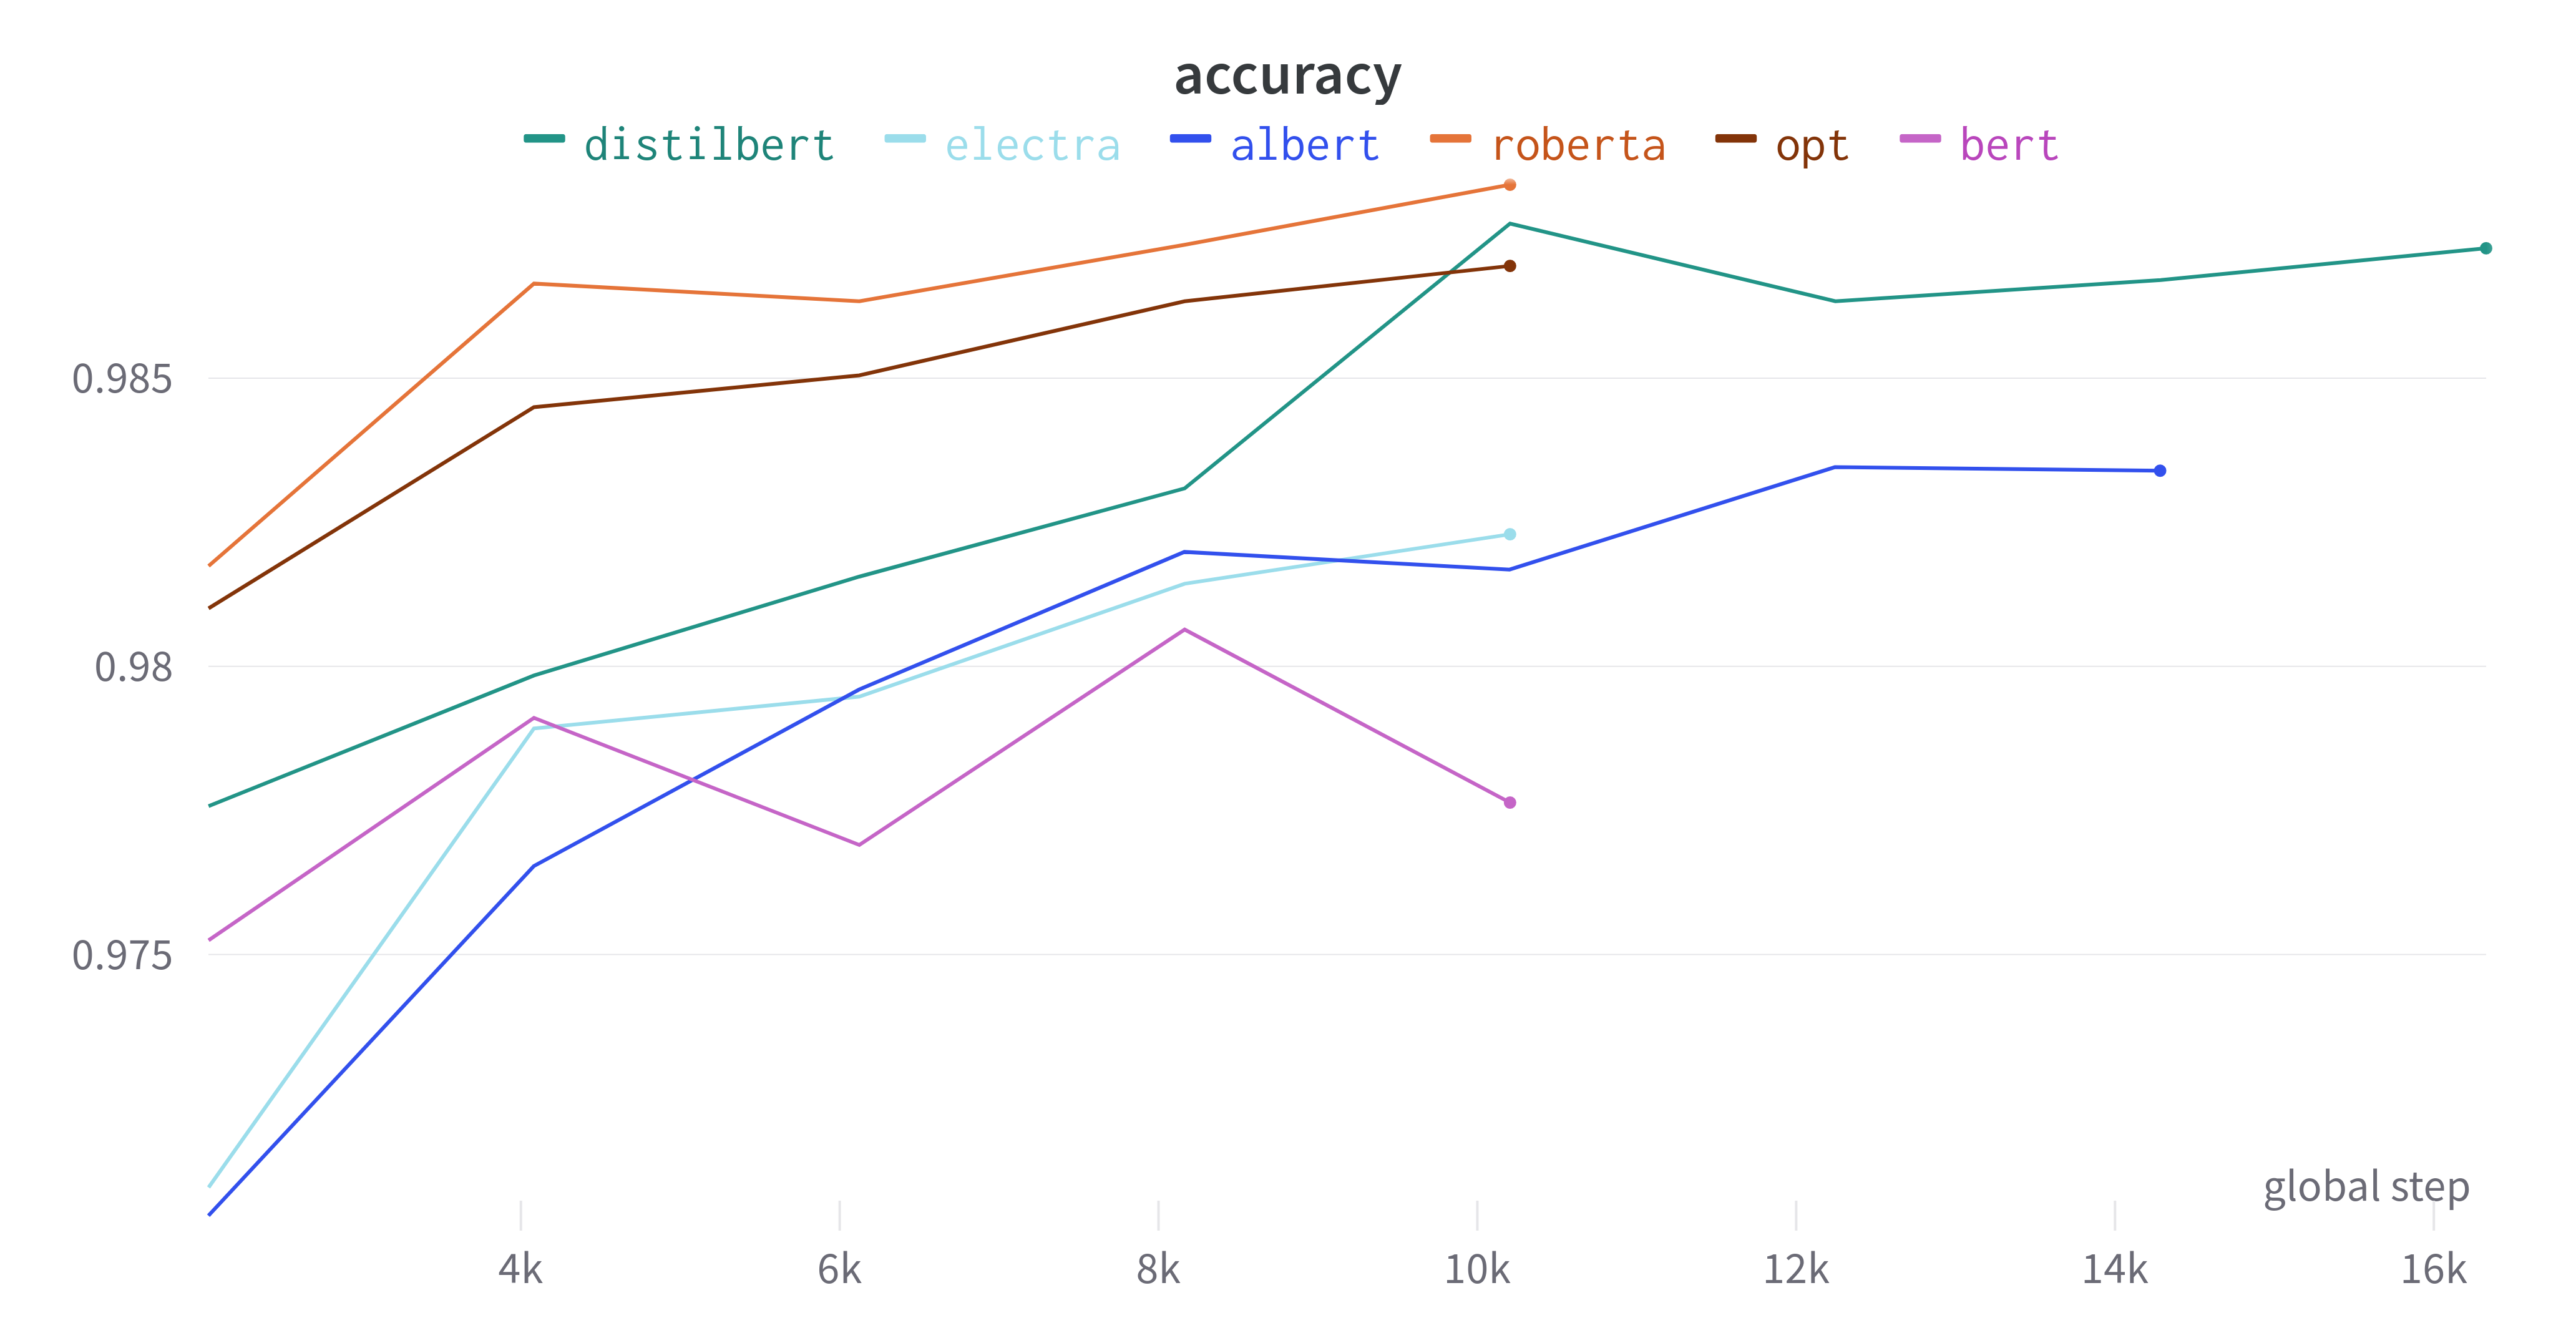
\includegraphics[width=.7\linewidth]{models/accuracy.png}
      \caption{График точности во время обучения моделей}
      \label{models-accuracy:image}
   \end{center}
\end{figure}

\begin{figure}[H]
   \begin{center}
      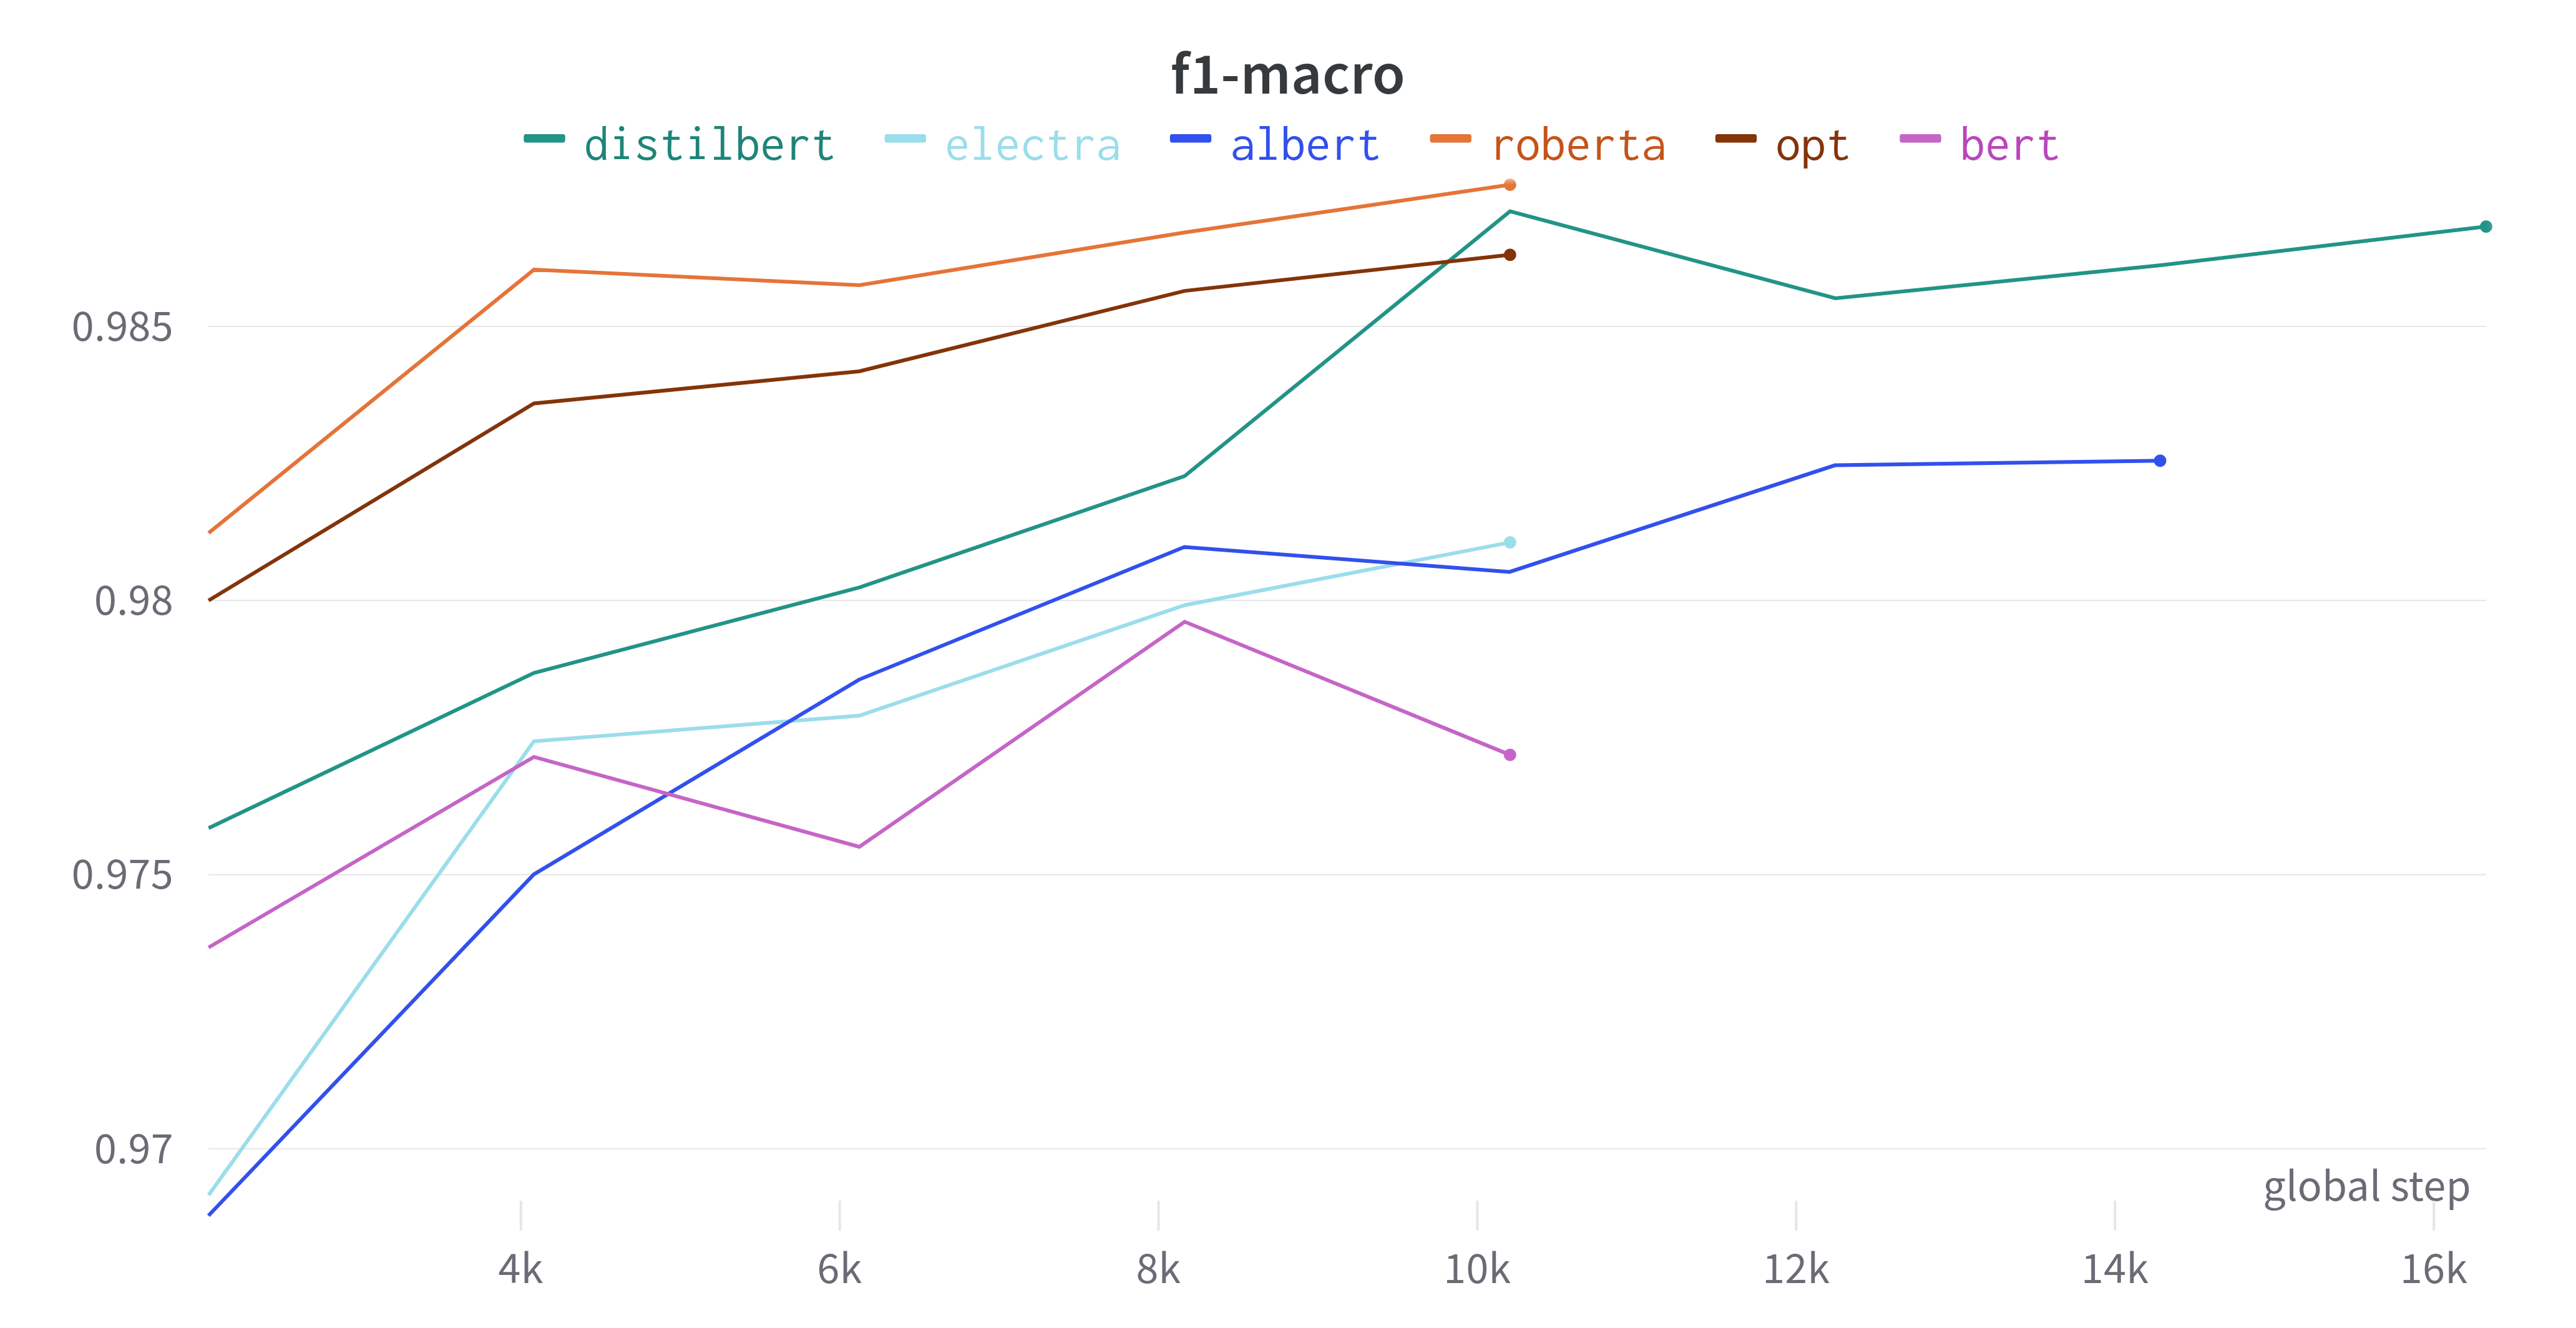
\includegraphics[width=.9\linewidth]{models/f1-macro.png}
      \caption{График macro $F_1$ во время обучения моделей}
      \label{f1-macro:image}
   \end{center}
\end{figure}

\begin{figure}[H]
   \begin{center} 
      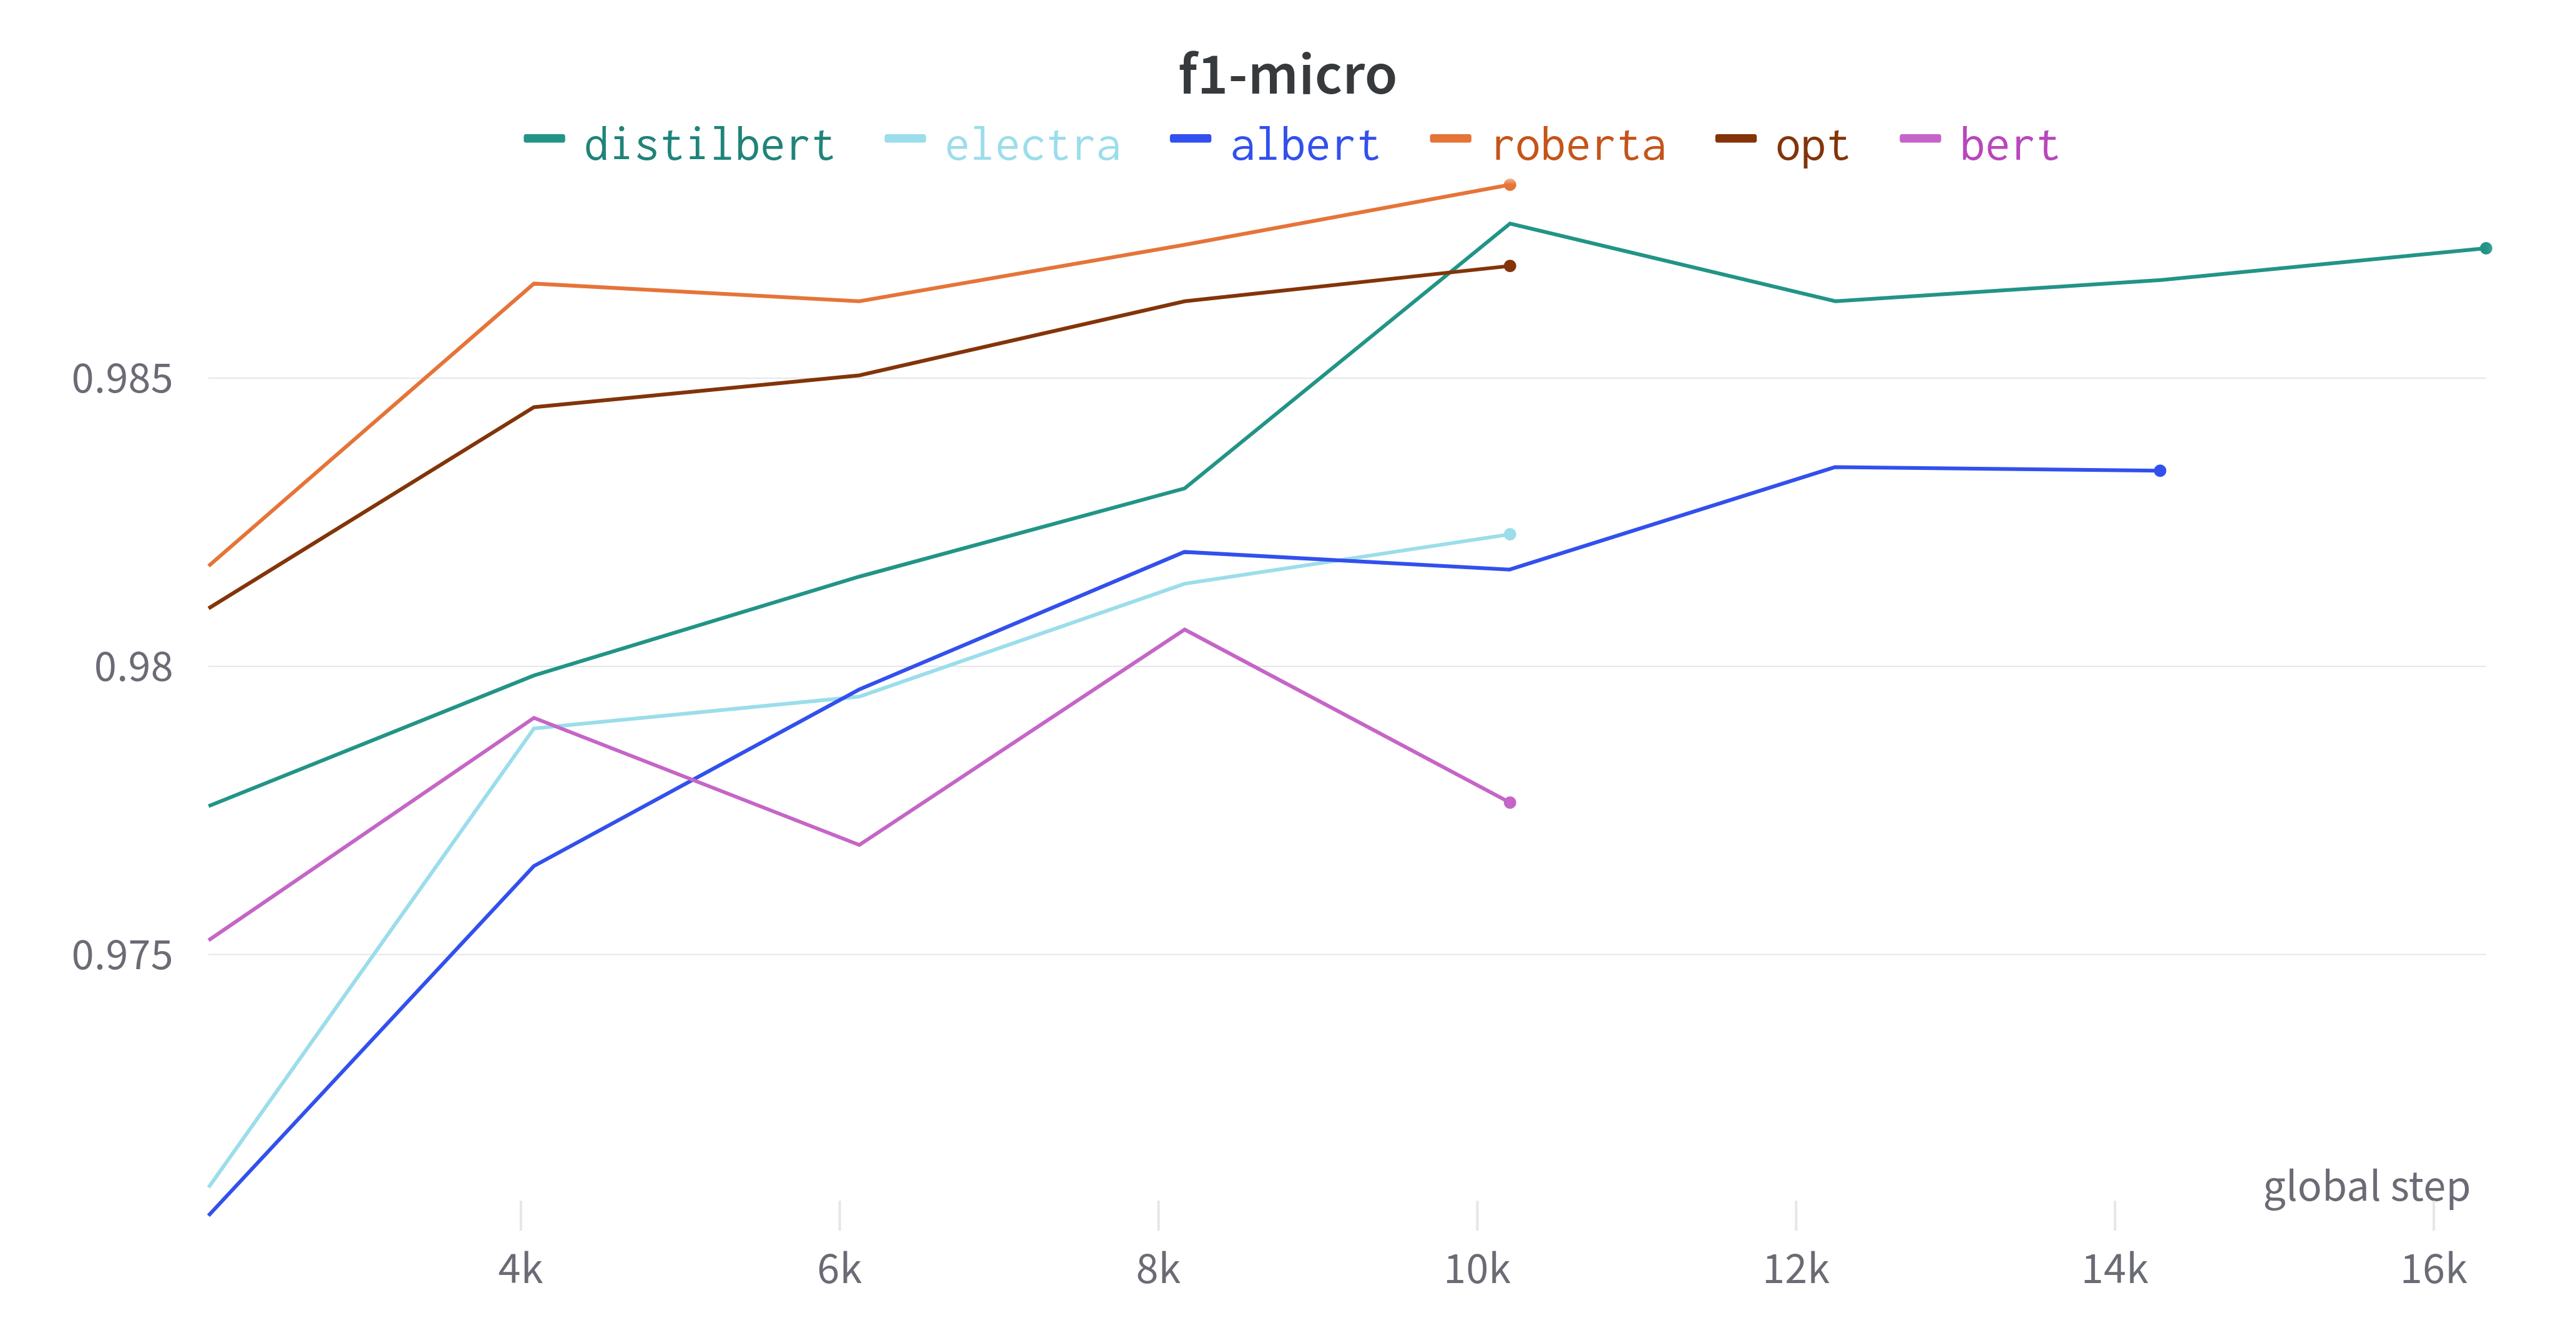
\includegraphics[width=.9\linewidth]{models/f1-micro.png}
      \caption{График micro $F_1$ во время обучения моделей}
      \label{f1-micro:image}
   \end{center} 
\end{figure}

По количеству занимаемой памяти и скорости обучения (рисунок \ref{gpu-memory:image}, рисунок \ref{train-runtime:image}) RoBERTa 
также является лучшей моделью. По количеству операций с плавающей точкой, затраченных на обучение 
(рисунок \ref{flos:image}), RoBERTa уступает лишь ALBERT и ELECTRA.  

\begin{figure}[H]
   \begin{center}
      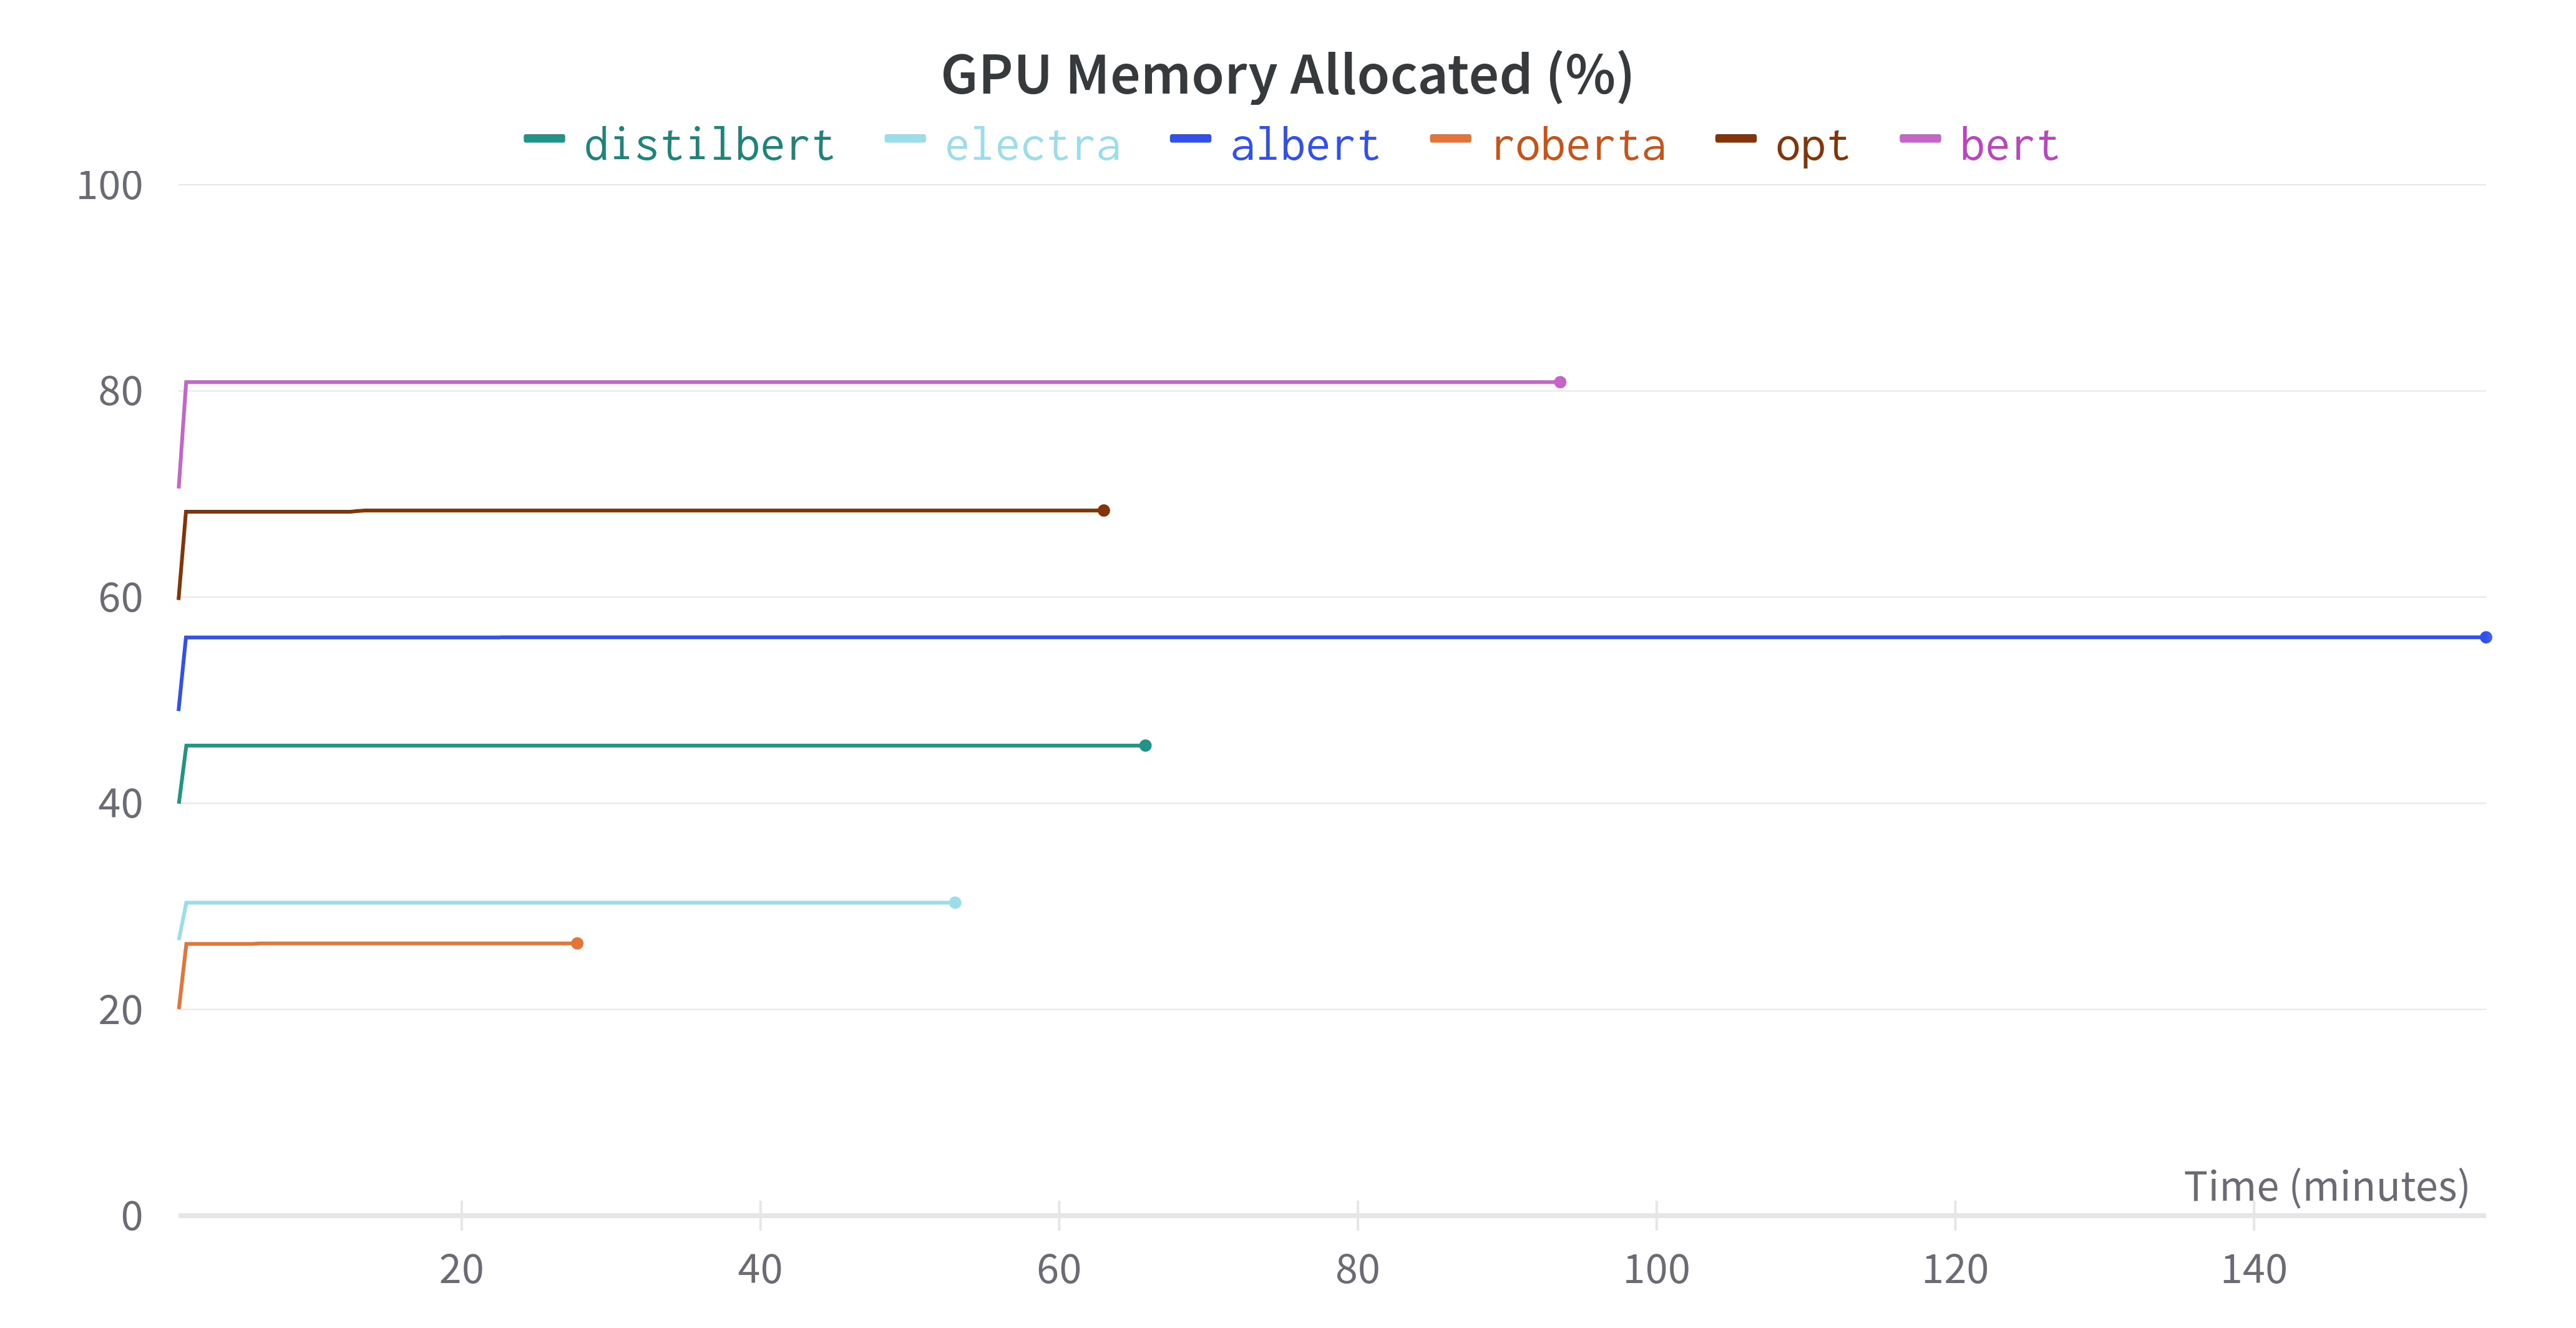
\includegraphics[width=\linewidth]{models/gpu-memory.png}
      \caption{Процент видеопамяти, занимаемый моделью при обучении}
      \label{gpu-memory:image}
   \end{center}
\end{figure}

\begin{figure}[H]
   \begin{center}
      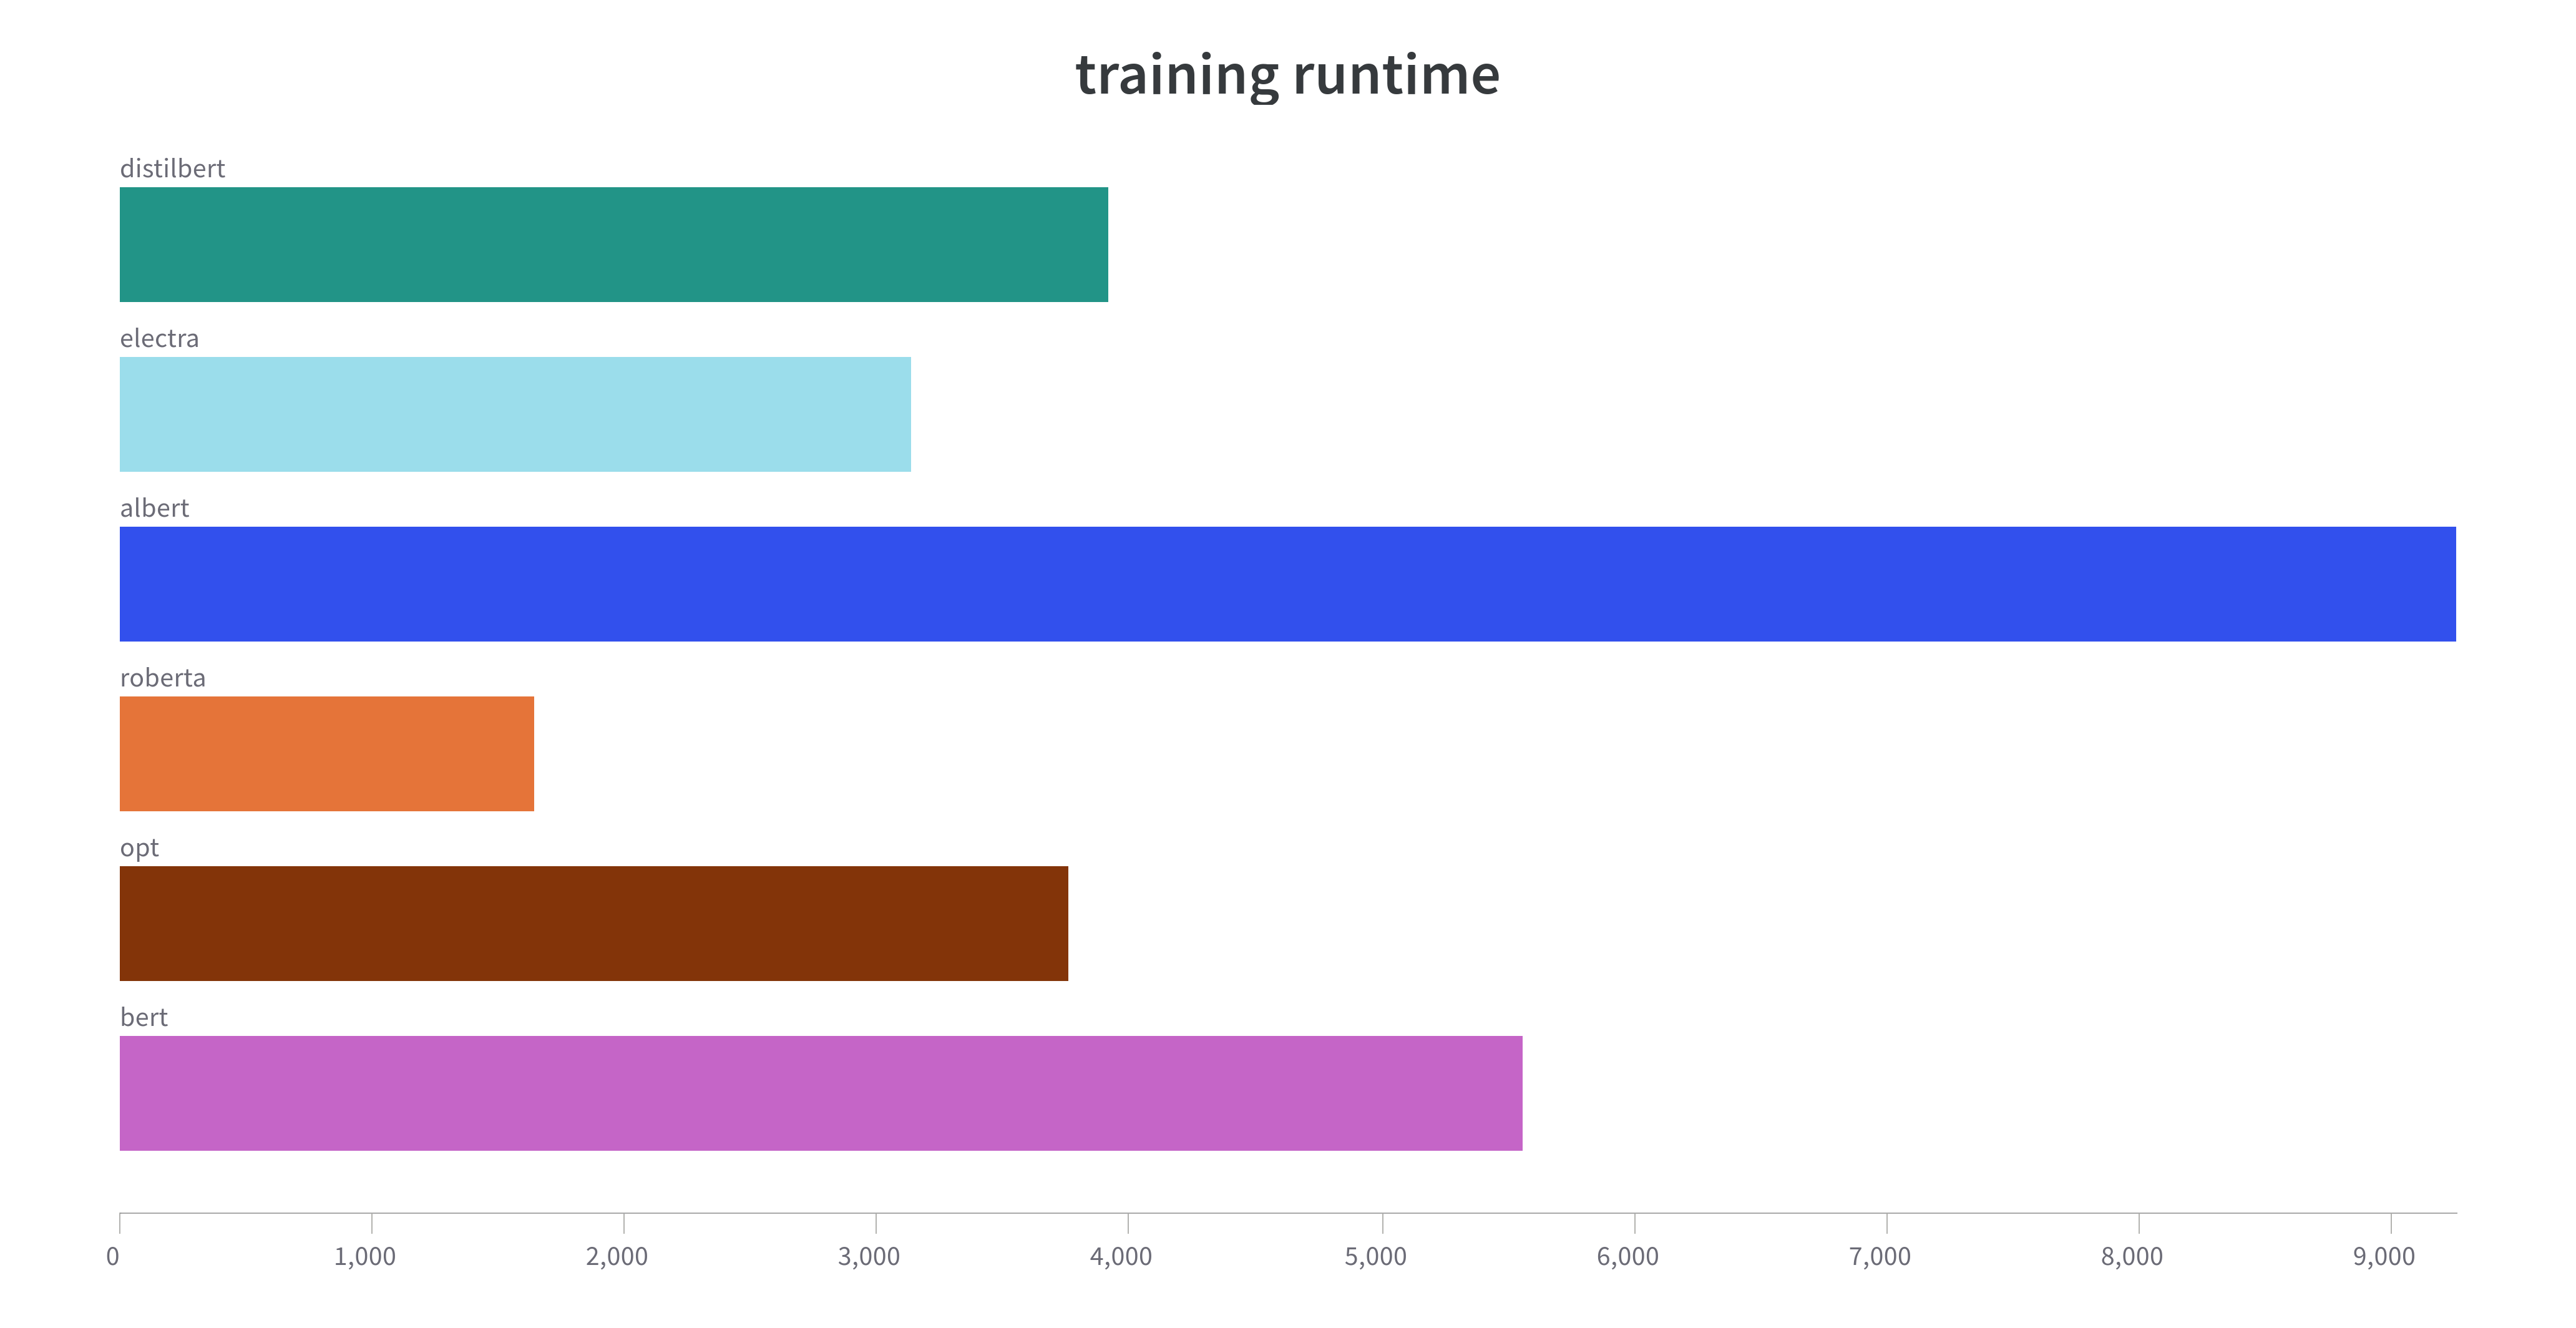
\includegraphics[width=\linewidth]{models/train-runtime.png}
      \caption{Время, затраченное на обучение}
      \label{train-runtime:image}
   \end{center}
\end{figure}

\begin{figure}[H]
   \begin{center}
      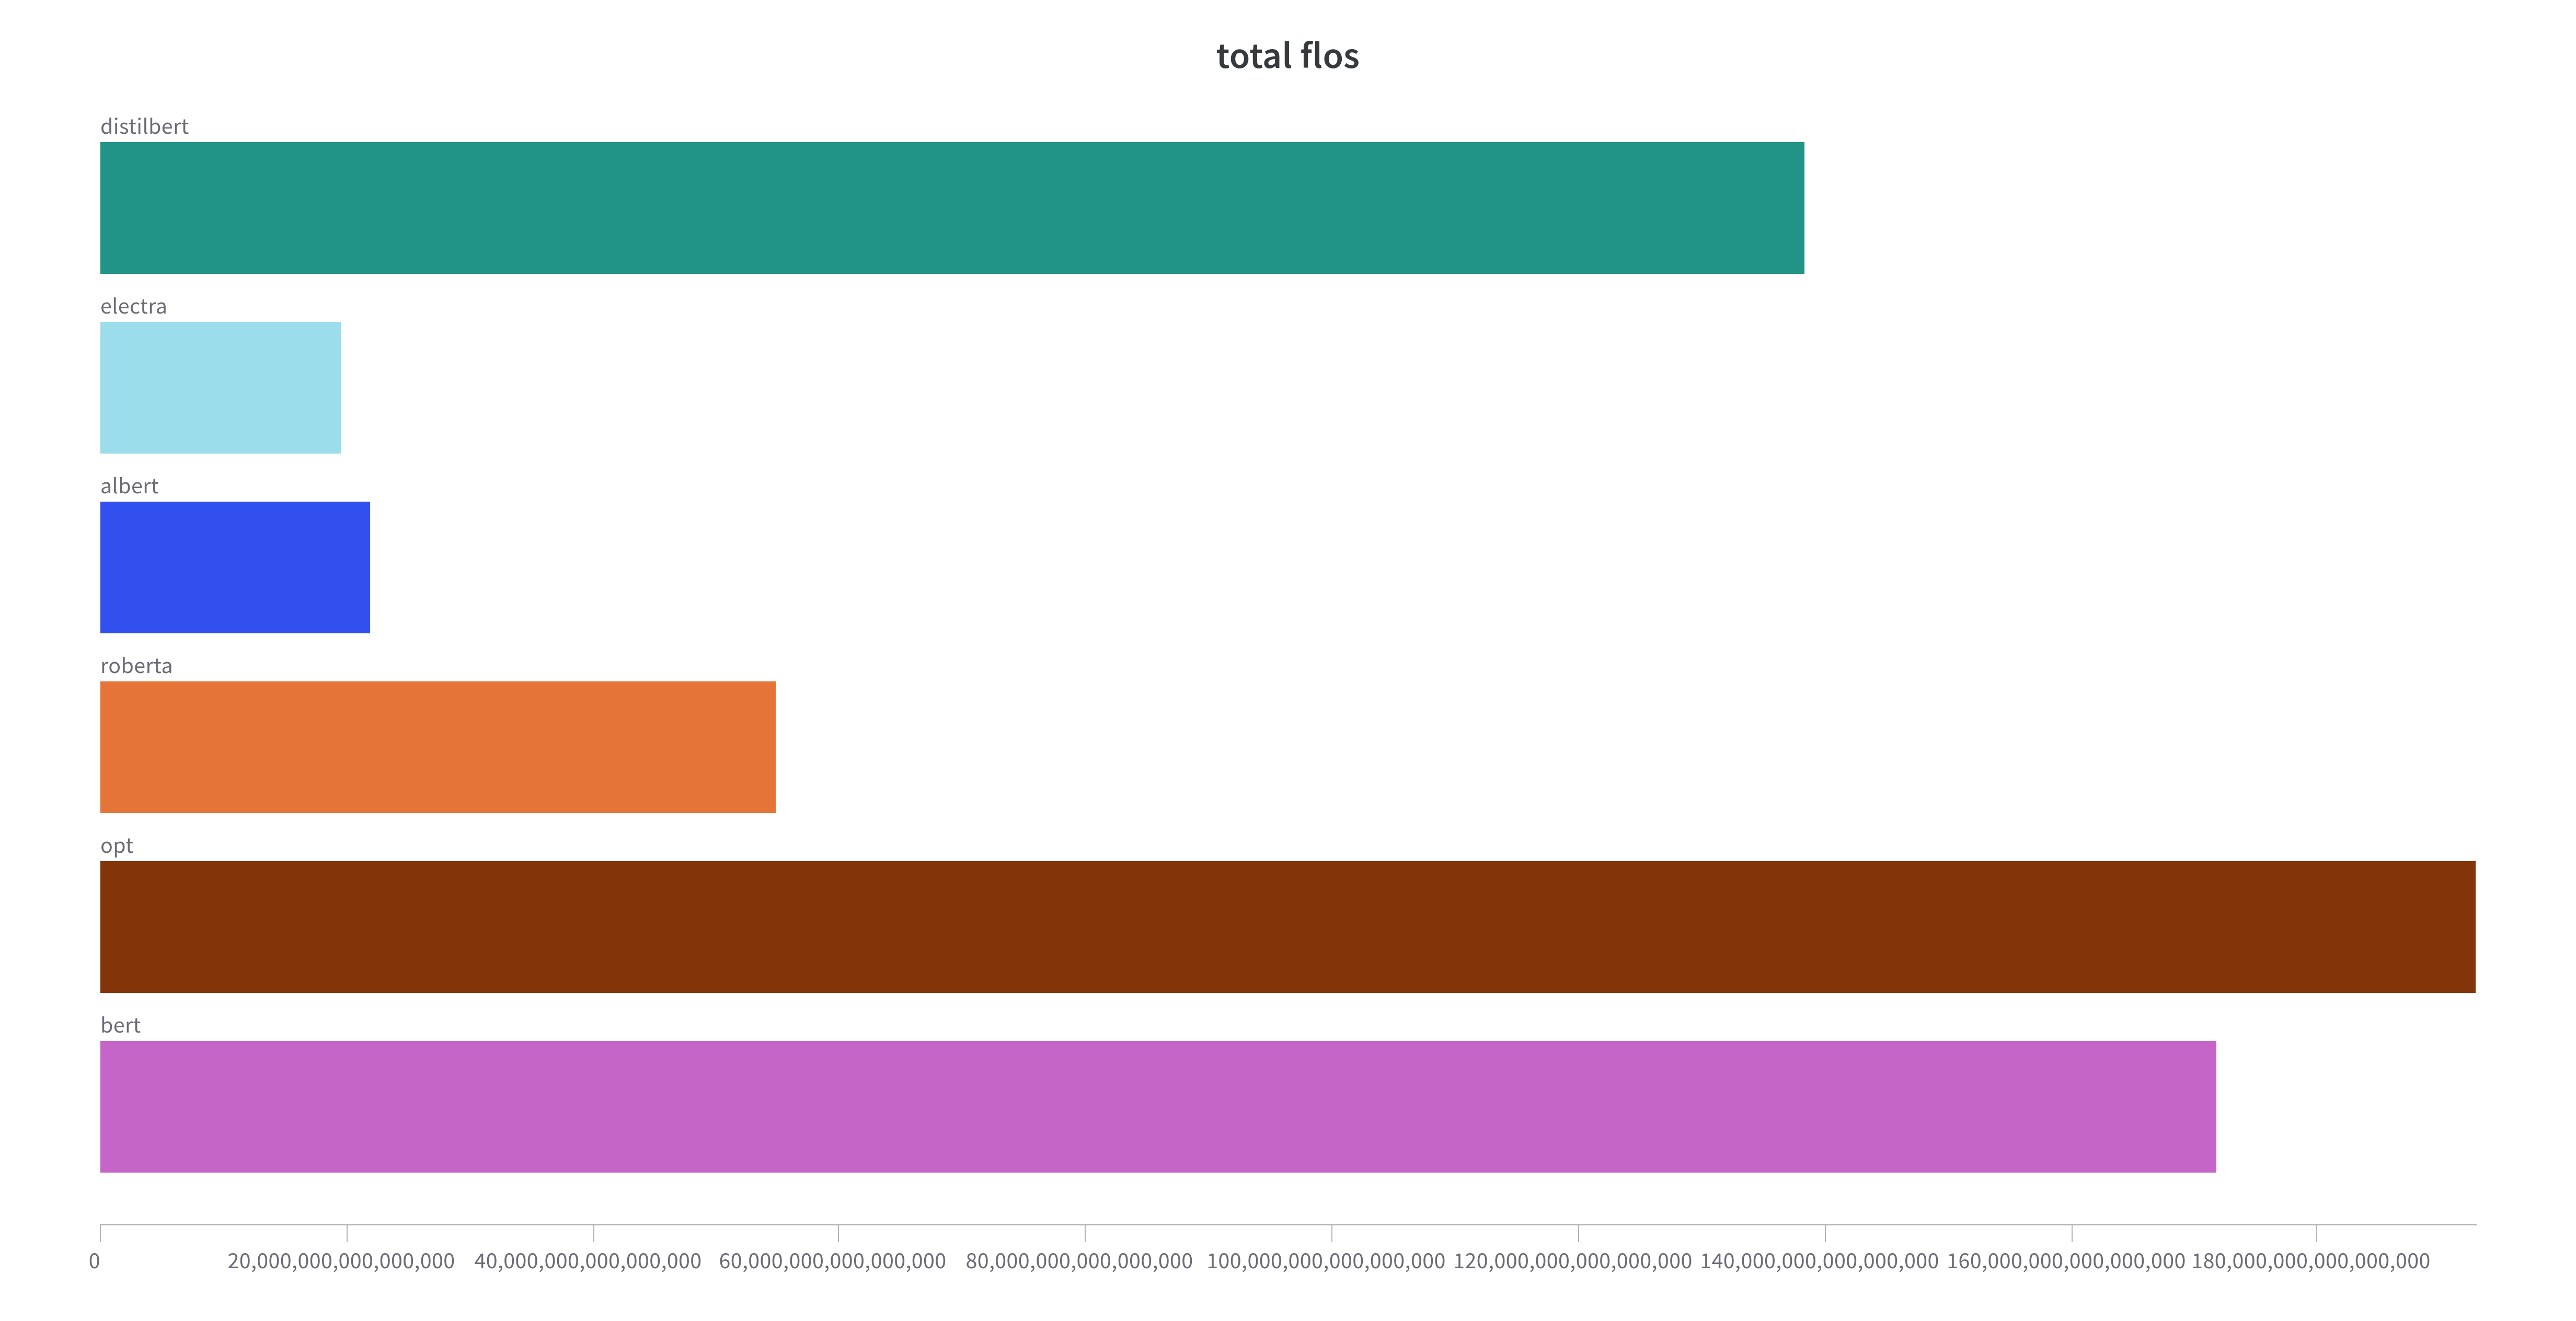
\includegraphics[width=\linewidth]{models/flos.png}
      \caption{Количество операций с плавающей точкой, затраченных на обучение}
      \label{flos:image}
   \end{center}
\end{figure}

По скорости при использовании (рисунок \ref{test-runtime:image}, рисунок \ref{test-samples:image}) RoBERTa также является наиболее оптимальной моделью. 

%\begin{figure}[H]
%   \begin{center}
%      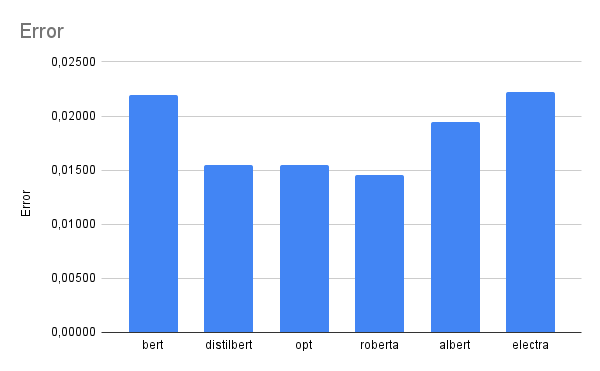
\includegraphics[width=.9\linewidth]{test/error.png}
%      \caption{Ошибка на тестовых данных}
%      \label{test-accuracy:image}
%   \end{center}
%\end{figure}

%\begin{figure}[H]
%   \begin{center}
%      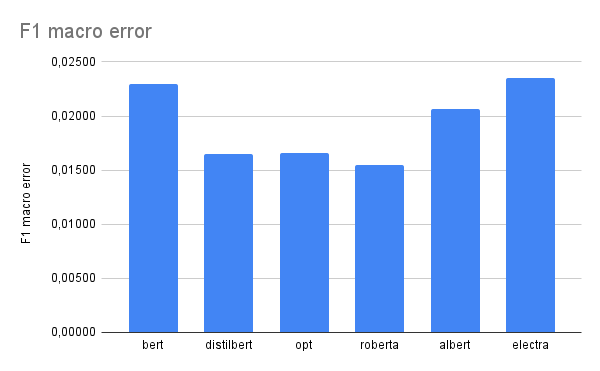
\includegraphics[width=.9\linewidth]{test/f1-macro-error.png}
%      \caption{Ошибка macro $F_1$ на тестовых данных}
%      \label{test-f1-macro:image}
%   \end{center}
%\end{figure}

%\begin{figure}[H]
%   \begin{center}
%      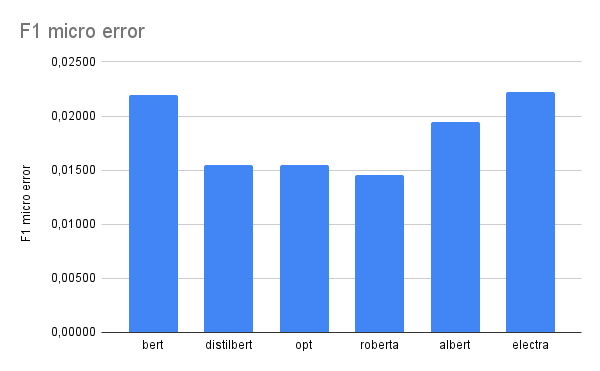
\includegraphics[width=.9\linewidth]{test/f1-micro-error.png}
%      \caption{Ошибка micro $F_1$ на тестовых данных}
%      \label{test-f1-micro:image} 
%   \end{center}
%\end{figure}

\begin{figure}[H]
   \begin{center}
      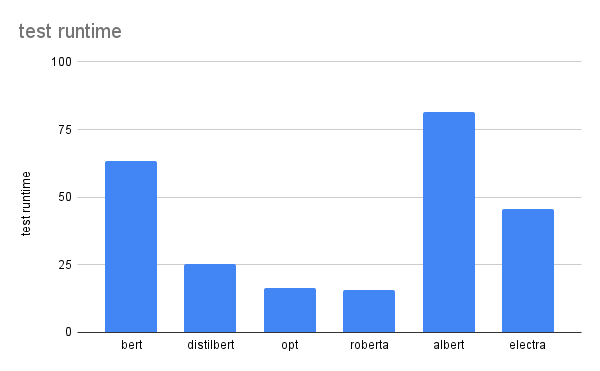
\includegraphics[width=.9\linewidth]{test/test runtime.png}
      \caption{Время, затраченное на тестирование}
      \label{test-runtime:image}
   \end{center}
\end{figure}

\begin{figure}[H]
   \begin{center}
      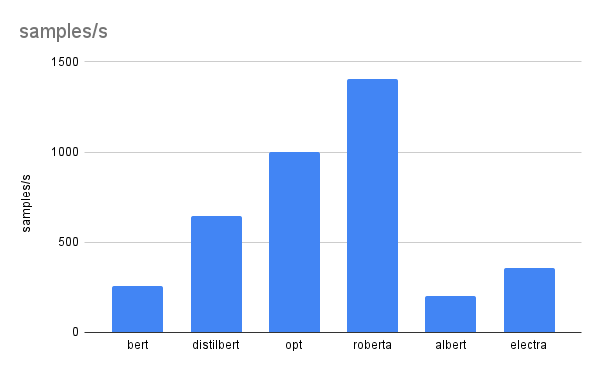
\includegraphics[width=.9\linewidth]{test/samples_s.png}
      \caption{Скорость при тестировании}
      \label{test-samples:image}
   \end{center}
\end{figure}

График функции ошибки во время обучения и график функции ошибки на валидационных данных можно 
найти в приложении \ref{app:models}.

\section{ТЕСТИРОВАНИЕ И ПРИМЕРЫ РАБОТЫ ИТОГОВОЙ МОДЕЛИ}
Проанализировав метрики на тестовых данных (таблица \ref{test-metrics:table}) и примеры работы итоговой модели выделения интентов (таблица \ref{test-examples:table}) можно сделать вывод, что модель неплохо справляется с поставленной задачей, однако наличие неправильно классифицированных интентов может говорить о неполноте данных и сложности в различении некоторых интентов. Например, вопросы <<Как дела?>> или <<Что нового?>> в английском языке могут использоваться в качестве приветствия. Отдельной проблемой является распознавание шуток. Это требует дальнейшей работы над обучающим набором данных для улучшения итогового результата.
\begin{table}[H]
   \captionsetup{format=hang, singlelinecheck=false}
   \raggedleft
      \caption{Метрики на тестовых данных}
      \label{test-metrics:table}
   \centering        
   \begin{tabular}{|p{4cm}|p{4cm}|}
      \hline
      Accuracy & 98,54\% \\
      \hline
      Micro $F_1$ & 98,54\% \\
      \hline
      Macro $F_1$ & 98,45\% \\
      \hline
   \end{tabular}
\end{table}

\begin{table}[H]
   \captionsetup{format=hang, singlelinecheck=false}
   \raggedleft
      \caption{Примеры работы итоговой модели}
      \label{test-examples:table}
   \centering        
   \begin{tabular}{|p{8cm}|p{8cm}|}
      \hline
      Примеры & Предсказанные классы примеров \\
      \hline
      Hello, Jack! & Greeting \\
      \hline
      I want you to attack that people. & Attack \\
      \hline
      Can i buy something from you? & Exchange \\
      \hline
      1234 & Drival \\
      \hline
      Is here job for me? & Receive quest \\
      \hline
      I'm going to hurt you! & Threat \\
      \hline
      Can you deliver this message to capital? & Message \\
      \hline
      What can you tell me about this lands? & Knowledge \\
      \hline
      Goodbye, my friend! & Farewell \\
      \hline
      fight can low be common & Drival \\
      \hline
      Follow me. & Follow \\
      \hline
      How are you today? & Greeting \\
      \hline
      What are you doing today? & Greeting \\
      \hline
      How are you today? & Greeting \\
      \hline
      What are you doing here? & Knowledge \\
      \hline
      Can you help me? & Join \\
      \hline
      Why is the chicken crossing the road? & Knowledge \\
      \hline
   \end{tabular}
\end{table}


\addchap{ЗАКЛЮЧЕНИЕ}
	\begin{itemize}
   \item Изучены методы генерации и аугментирования данных, методы представления текстовых данных в векторном виде, методы машинного обучения для классификации текста в лице нейронных сетей, архитектуры моделей, наиболее часто используемых для обработки естественного языка и классификации текста в частности, программные средства для обучения и тестирования этих моделей, для логирования данных во время обучения и их анализа;
   \item Разработаны программы для генерации данных и проведения исследований;
   \item Создан новый набор данных;
   \item Проведены исследования для поиска оптимальных параметров для каждой выбранной модели и сравнения моделей между собой;
   \item Получена основная часть NLU модуля, а именно модель для классификации намерений. Наиболее оптимальной для этой задачи архитектурой является RoBERTa;
   \item Не самое высокое качество обучающего набора данных, что связано со сложностью выделения некоторых интентов и несовершенством искусственно сгенерированных и аугментированных данных.
\end{itemize}

%Таким образом, была получена основная часть NLU модуля, а именно модель для классификации намерений. Наиболее оптимальной для этой задачи архитектурой является RoBERTa. Для получения итоговой модели был создан новый набор данных, а также были проведены иследования для поиска оптимальных параметров для каждой выбранной модели и для сравнения моделей между собой. Для этого были изучены методы генерации и аугментирования данных, методы представления текстовых данных в векторном виде, методы машинного обучения для классификации текста в лице нейронных сетей, а также архитектуры моделей, наиболее часто используемых для обработки естественного языка и классификации текста в частности. Кроме того, были изучены программные средства для обучения, тестирования этих моделей, логгирования данных во время обучения и их анализа, а также разработаны программы для генерации данных и проведения исследования.

%Однако по результатам тестирования модели, можно сделать вывод о не самом высоком качестве обучающего набора данных, что связано со сложностью выделения некоторых интентов и несовершенством искусственно сгенерированных и аугментированных данных, что требует дальнешей работы в этом направлении.

\break

\begin{thebibliography}{00}
   \addcontentsline{toc}{chapter}{СПИСОК ЛИТЕРАТУРЫ}
   \bibitem{bayes}
     \textit{Rish I. et al.} An empirical study of the naive Bayes classifier // IJCAI 2001 workshop on empirical methods in artificial intelligence. – 2001. – Т. 3. – №. 22. – С. 41-46.
   \bibitem{svm}
     \textit{Cortes C., Vapnik V.} Support-vector networks // Machine learning. – 1995. – Т. 20. – С. 273-297.
   \bibitem{gelu}
     \textit{Hendrycks D., Gimpel K.} Gaussian error linear units (gelus) // arXiv preprint arXiv:1606.08415. – 2016 (дата обр. 13.06.2023).
   \bibitem{backprop}
     \textit{Hecht-Nielsen R.} Theory of the backpropagation neural network // Neural networks for perception. – Academic Press, 1992. – С. 65-93.
   \bibitem{transformers}
     \textit{Vaswani A. et al.} Attention is all you need // Advances in neural information processing systems. – 2017. – Т. 30.
   \bibitem{bert}
     \textit{Devlin J. et al.} Bert: Pre-training of deep bidirectional transformers for language understanding // arXiv preprint arXiv:1810.04805. – 2018 (дата обр. 13.06.2023).
   \bibitem{roberta}
     \textit{Liu Y. et al.} Roberta: A robustly optimized bert pretraining approach // arXiv preprint arXiv:1907.11692. – 2019 (дата обр. 13.06.2023).
   \bibitem{distilbert}
     \textit{Sanh V. et al.} DistilBERT, a distilled version of BERT: smaller, faster, cheaper and lighter // arXiv preprint arXiv:1910.01108. – 2019 (дата обр. 13.06.2023).
   \bibitem{albert}
     \textit{Lan Z. et al.} Albert: A lite bert for self-supervised learning of language representations // arXiv preprint arXiv:1909.11942. – 2019 (дата обр. 13.06.2023).
   \bibitem{electra}
     \textit{Clark K. et al.} Electra: Pre-training text encoders as discriminators rather than generators // arXiv preprint arXiv:2003.10555. – 2020 (дата обр. 13.06.2023).
   \bibitem{opt}
     \textit{Zhang S. et al.} Opt: Open pre-trained transformer language models // arXiv preprint arXiv:2205.01068. – 2022 (дата обр. 13.06.2023).
   \bibitem{t5}
     \textit{Raffel C. et al.} Exploring the limits of transfer learning with a unified text-to-text transformer // The Journal of Machine Learning Research. – 2020. – Т. 21. – №. 1. – С. 5485-5551.
   \bibitem{open-assistant}
     \textit{Koepf A. et al.} OpenAssistant Conversations--Democratizing Large Language Model Alignment // arXiv preprint arXiv:2304.07327. – 2023 (дата обр. 13.06.2023).
   \bibitem{paper}
     \textit{Бурлаков В. С., Ишутин М. А., Пятанин А. А.} Диалоговая система для разработчиков видеоигр // Наука. Технологии. Инновации : сб. науч. тр. : в 11 ч., Новосибирск, 05-08 дек. 2022 г. Ч. 2 -- Изд-во НГТУ, 2022. -- C. 101-104.
   \bibitem{py}
     Документация Python [Электронный ресурс]. URL: https://docs.python.org/3/ (дата обр. 13.06.2023).
   \bibitem{pd}
     Документация Pandas [Электронный ресурс]. URL: https://pandas.pydata.org/docs/ (дата обр. 13.06.2023).
   \bibitem{transformer}
     Документация Transformers [Электронный ресурс]. URL: https://huggingface.co/docs/transformers/index (дата обр. 13.06.2023).
   \bibitem{datasets}
     Документация Datasets [Электронный ресурс]. URL: https://huggingface.co/docs/datasets/index (дата обр. 13.06.2023).
   \bibitem{evaluate}
     Документация Evaluate [Электронный ресурс]. URL: https://huggingface.co/docs/evaluate/index (дата обр. 13.06.2023).
   \bibitem{wandb}
     Документация Weights\&Biases [Электронный ресурс]. URL: https://docs.wandb.ai/ (дата обр. 13.06.2023).
   \bibitem{tqdm}
     Документация tqdm [Электронный ресурс]. URL: https://tqdm.github.io/ (дата обр. 13.06.2023).
   \bibitem{numpy}
     Документация NumPy [Электронный ресурс]. URL: https://numpy.org/doc/ (дата обр. 13.06.2023).
   \bibitem{matplotlib}
     Документация Matplotlib [Электронный ресурс]. URL: https://matplotlib.org/stable/index.html (дата обр. 13.06.2023).
   \end{thebibliography}

\appendix
\renewcommand{\thechapter}{\Asbuk{chapter}}
\chapter{ФРАГМЕНТ ПРОГРАММЫ ДЛЯ ГЕНЕРАЦИИ ДАННЫХ}
  \label{app:data-generating}\texttt{\lstinputlisting[language={Python}, caption=Фрагмент программы для генерации данных]{./code_sources/data-generating.py}}

\chapter{ТЕКСТ ПРОГРАММЫ ДЛЯ ПОИСКА ОПТИМАЛЬНЫХ ПАРАМЕТРОВ}
  \label{app:example}\texttt{\lstinputlisting[caption=Текст программы для проведения серии экспериментов, language={Python}]{./code_sources/bert-sweep.py}}

\chapter{ТЕКСТ ПРОГРАММЫ ДЛЯ СРАВНЕНИЯ МОДЕЛЕЙ}
  \label{app:train}\texttt{\lstinputlisting[language={Python}, caption=Программа для обучения модели]{./code_sources/train-bert.py}}

\chapter{ГРАФИКИ ПРИ ПОИСКЕ ОПТИМАЛЬНЫХ ПАРАМЕТРОВ}
  \label{app:sweeps}\begin{figure}[!htb] 
   \begin{minipage}{0.48\textwidth} 
     \centering 
     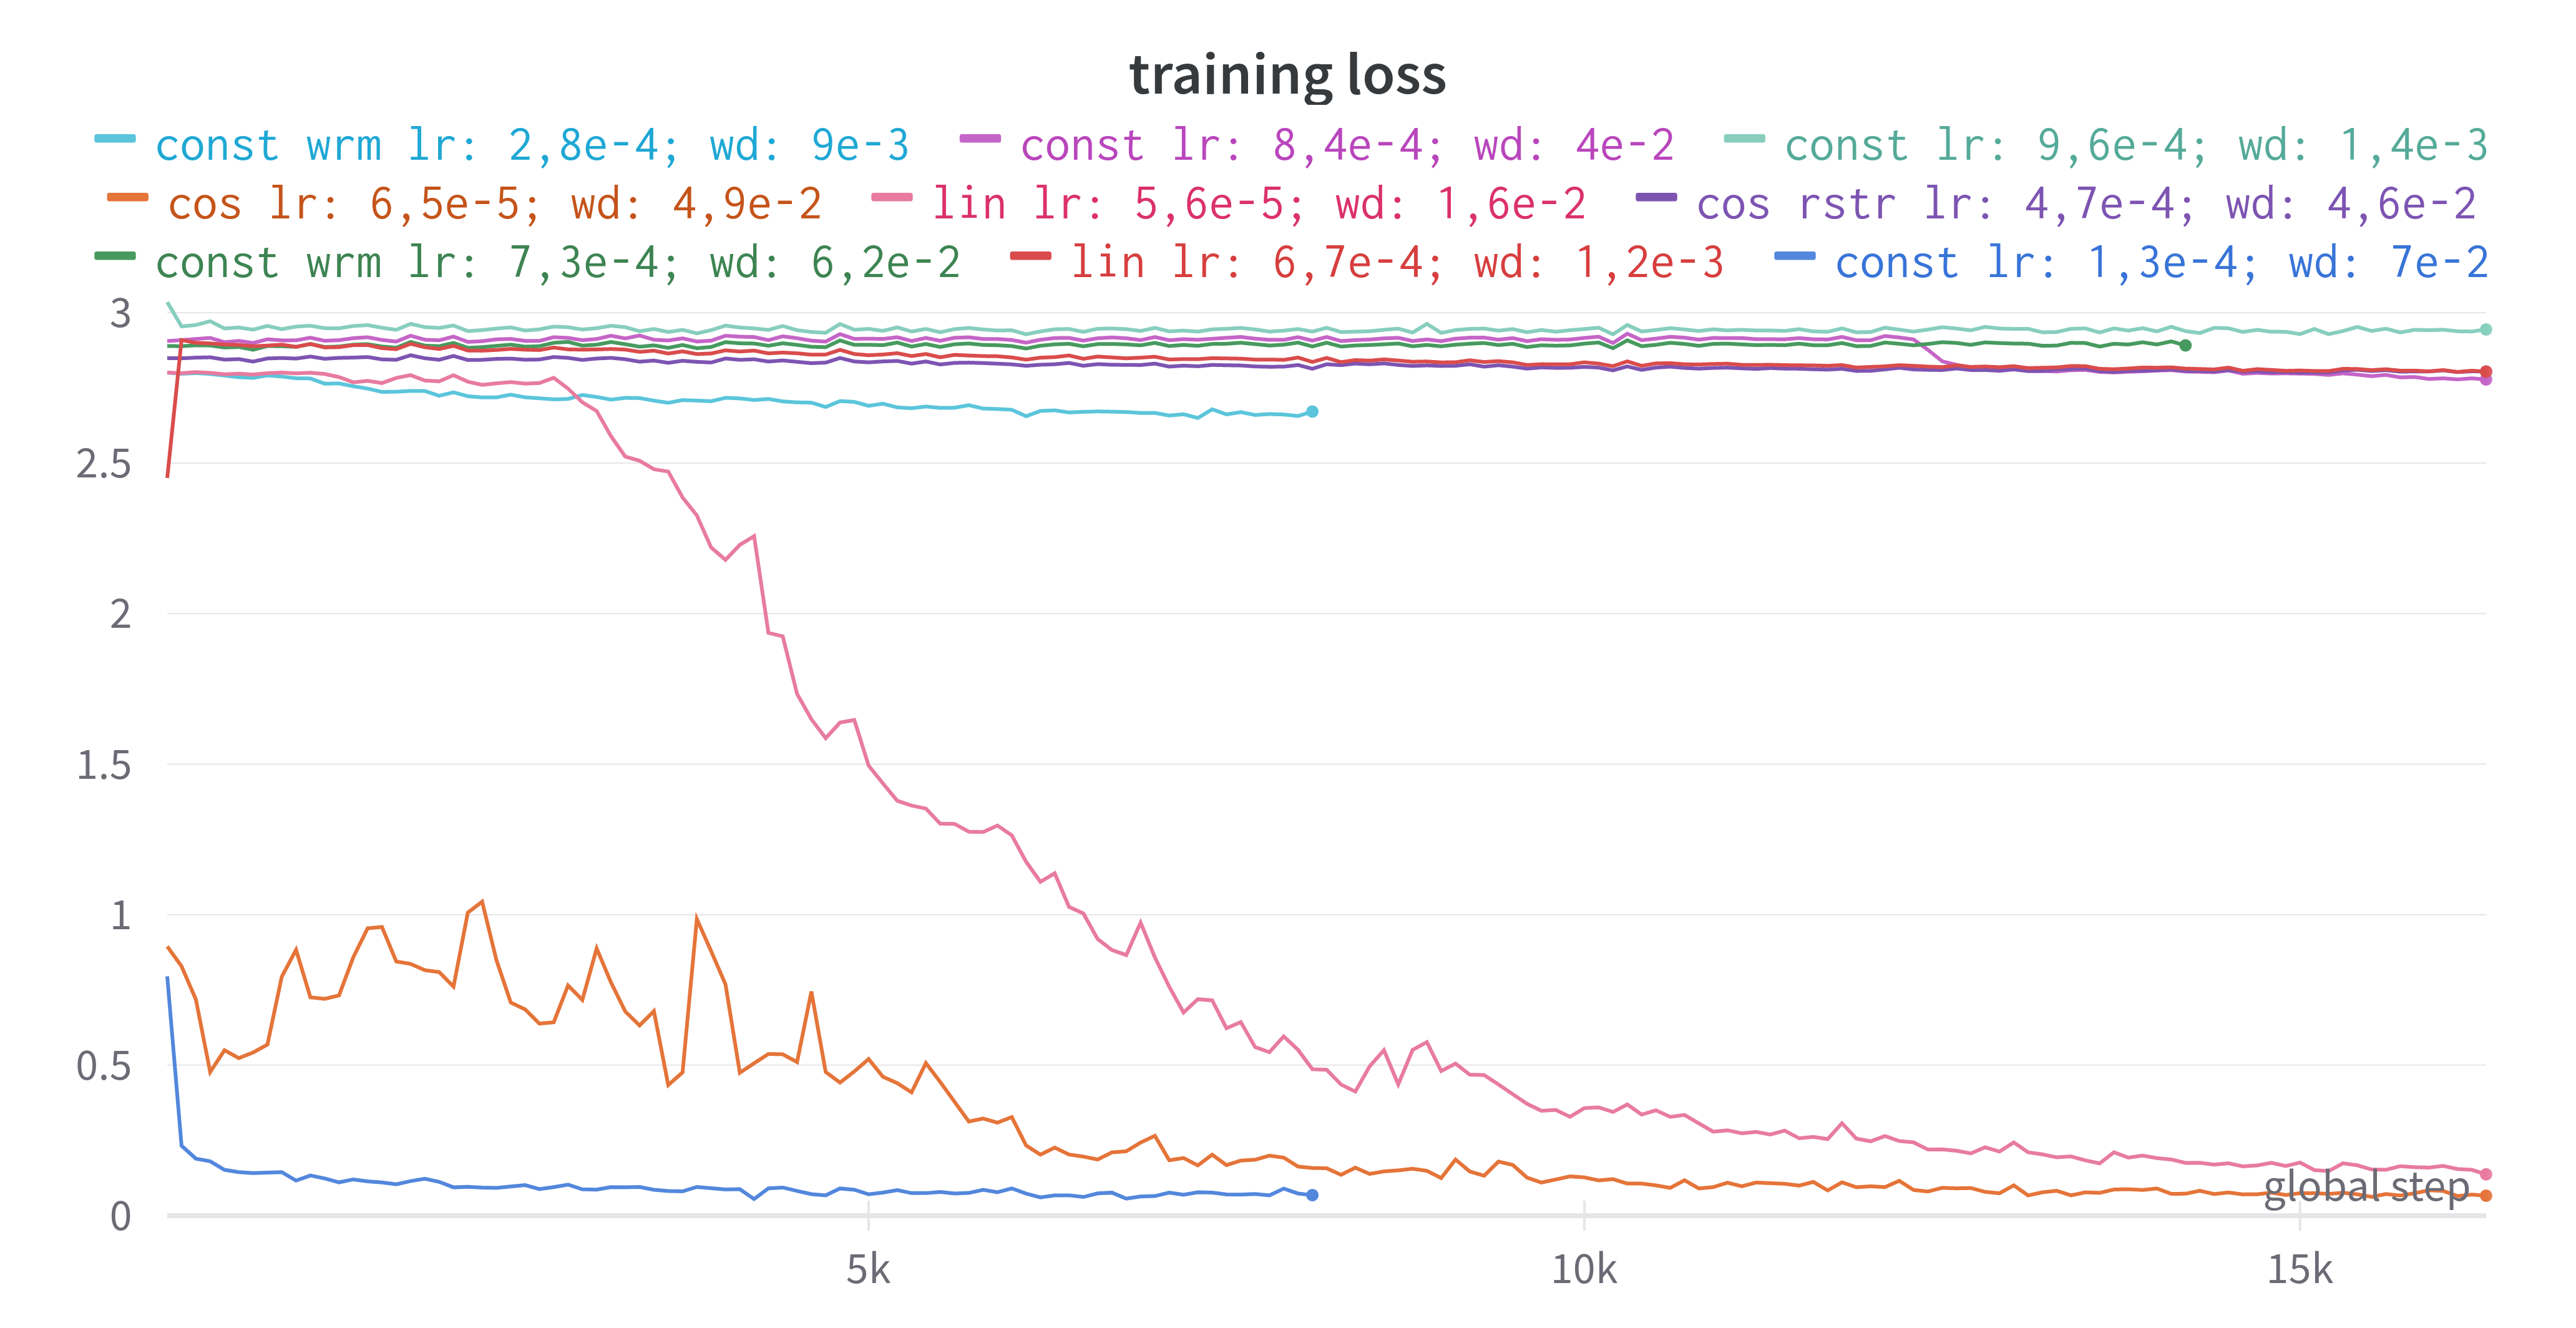
\includegraphics[width=\linewidth]{bert/train-loss.png}
     \caption{График функции ошибки во время обучения BERT} 
   \end{minipage}\hfill 
   \begin{minipage}{0.48\textwidth} 
     \centering 
     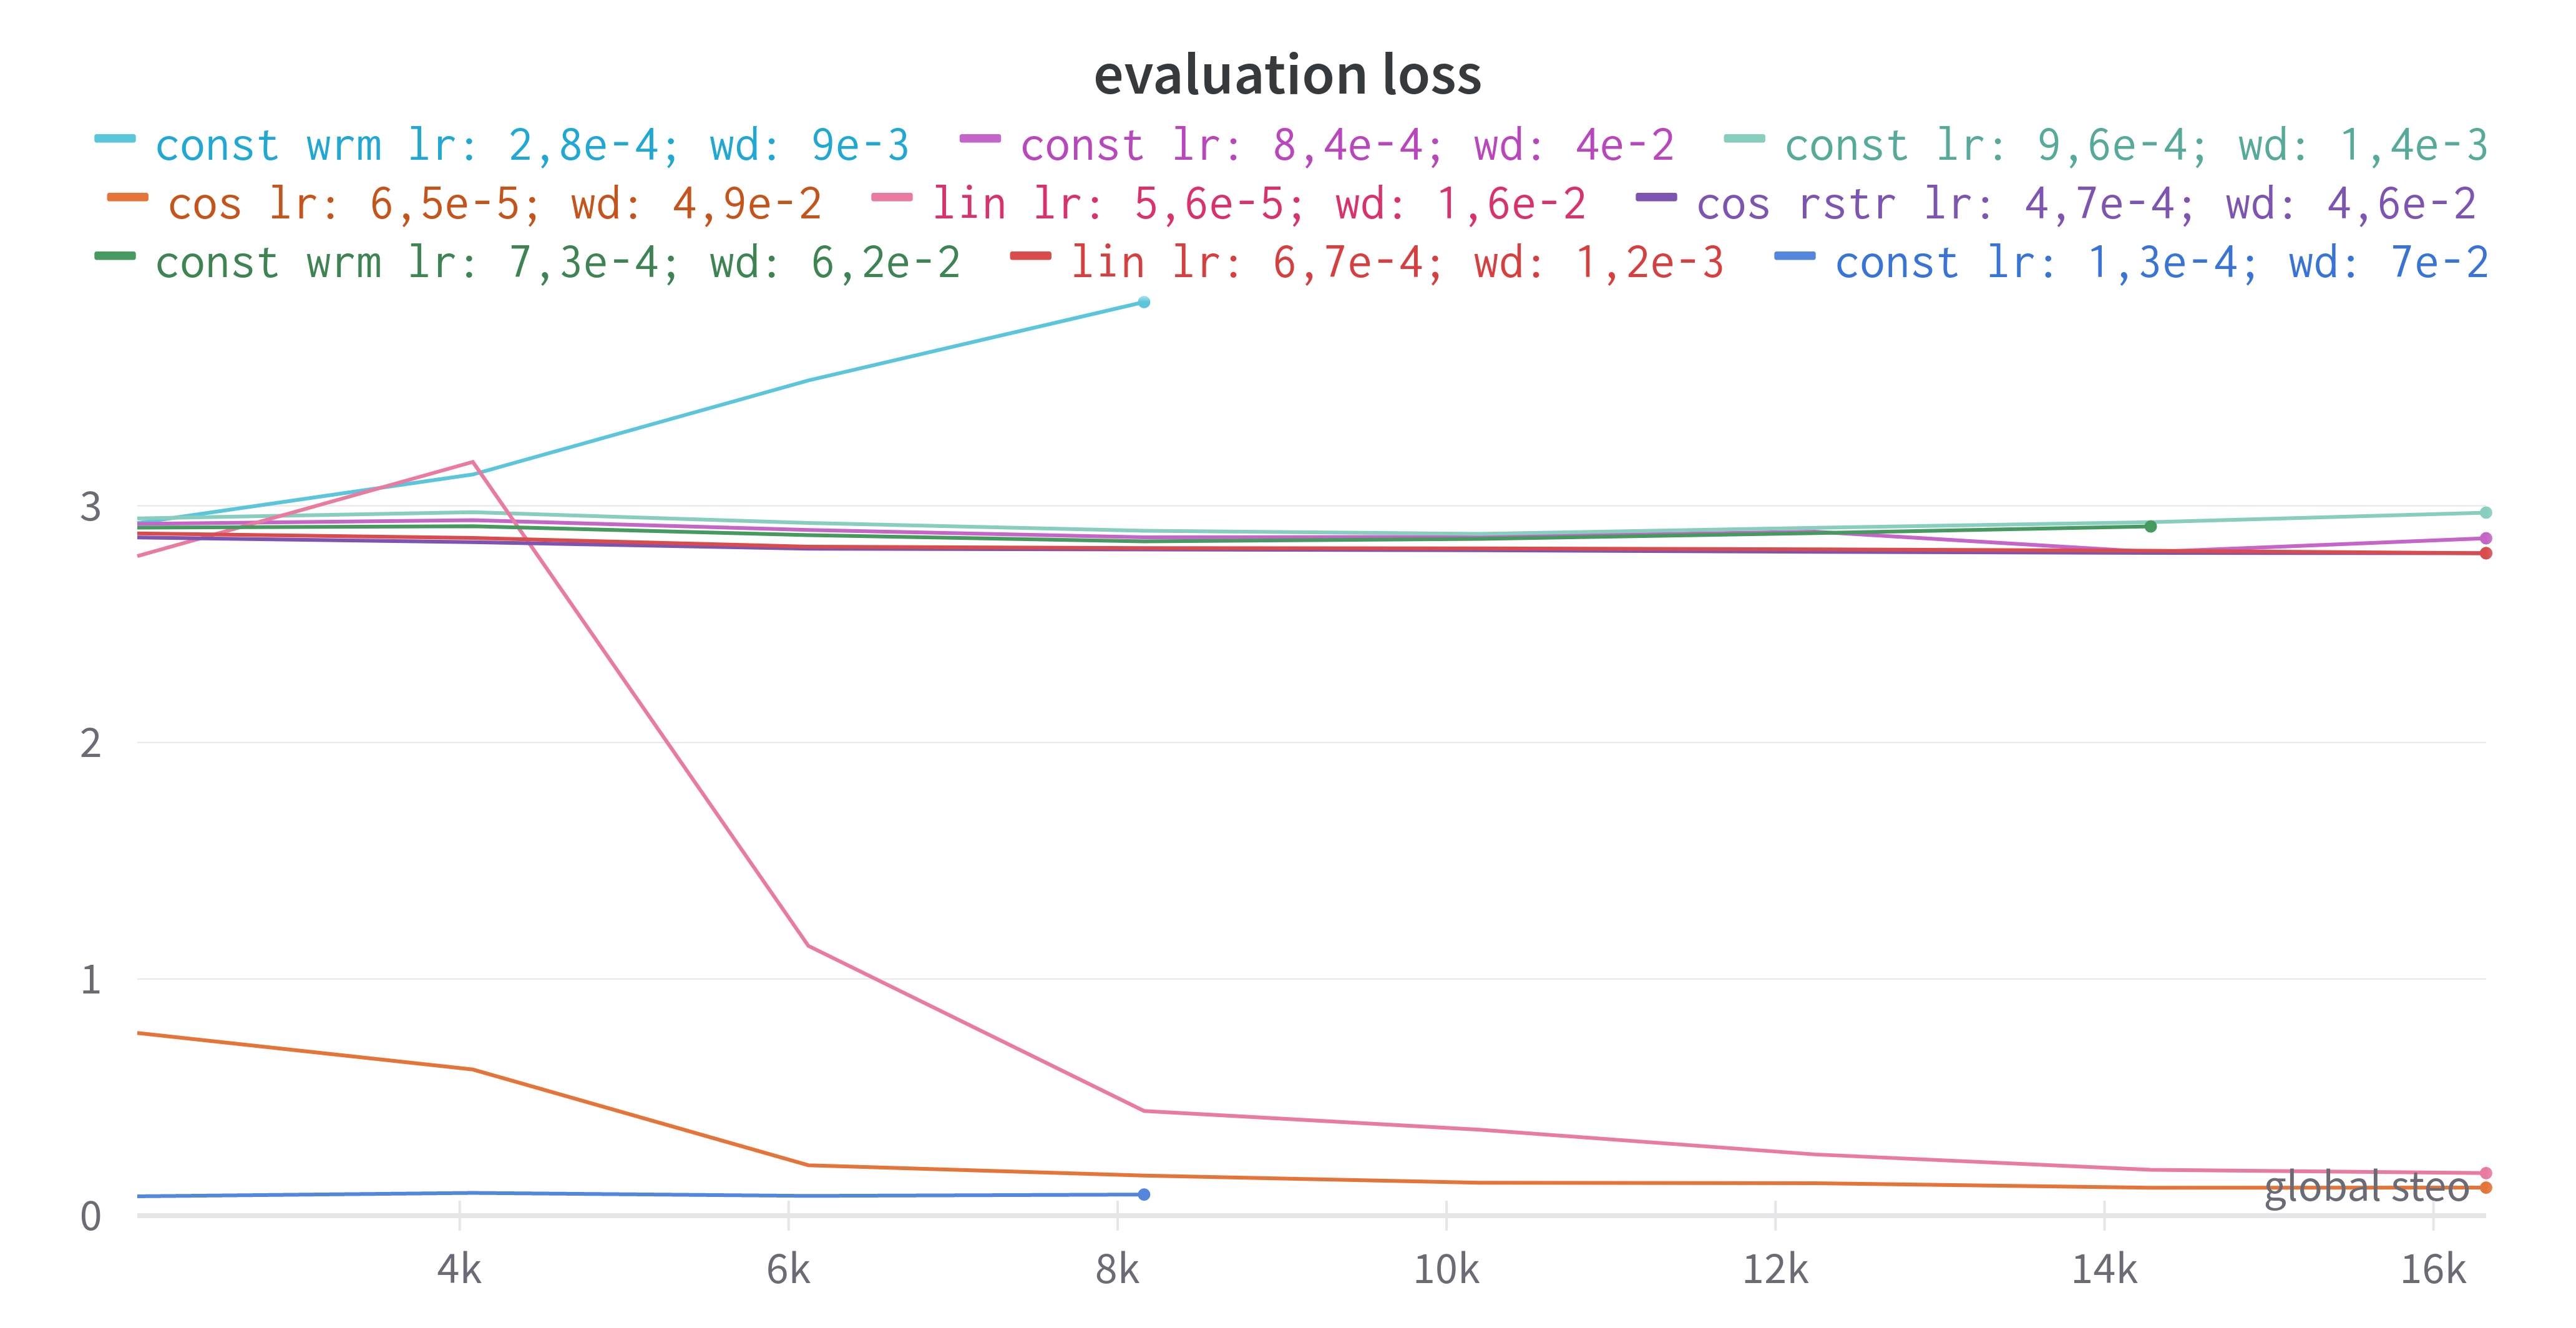
\includegraphics[width=\linewidth]{bert/eval-loss.png}
     \caption{График функции ошибки при валидации BERT} 
   \end{minipage} 
\end{figure}

\begin{figure}[!htb] 
   \begin{minipage}{0.48\textwidth} 
     \centering 
     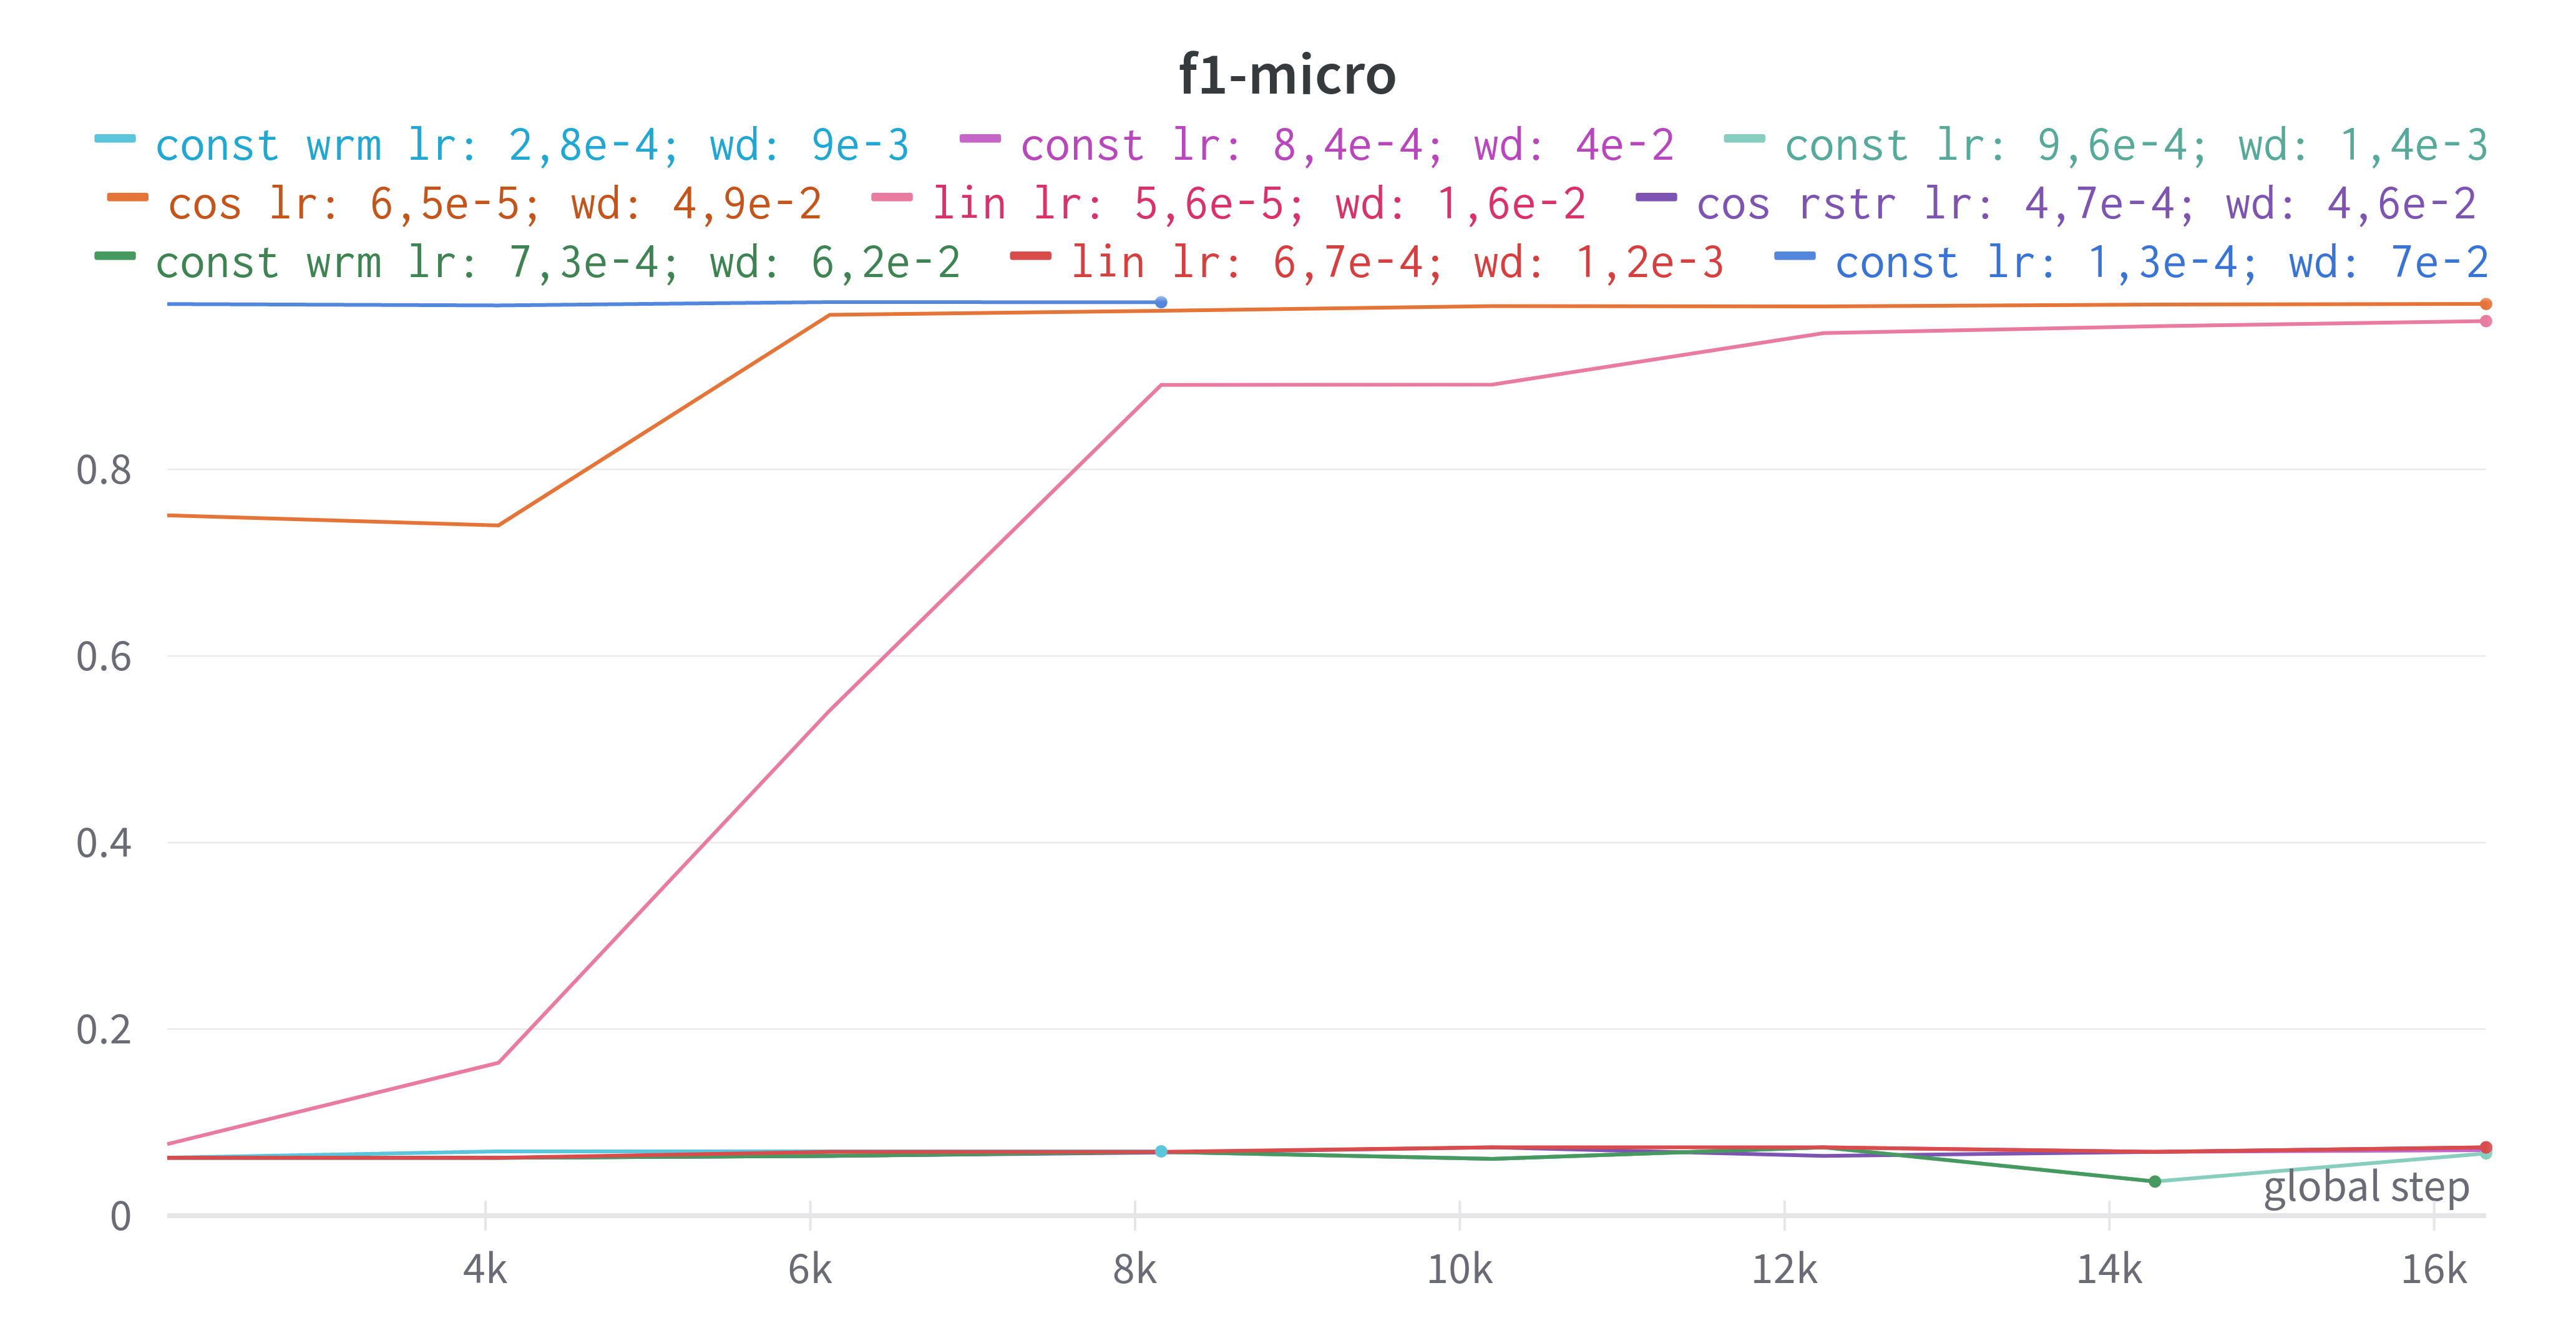
\includegraphics[width=\linewidth]{bert/f1-micro.png}
     \caption{Micro $F_1$ во время обучения BERT} 
   \end{minipage}\hfill 
   \begin{minipage}{0.48\textwidth} 
     \centering 
     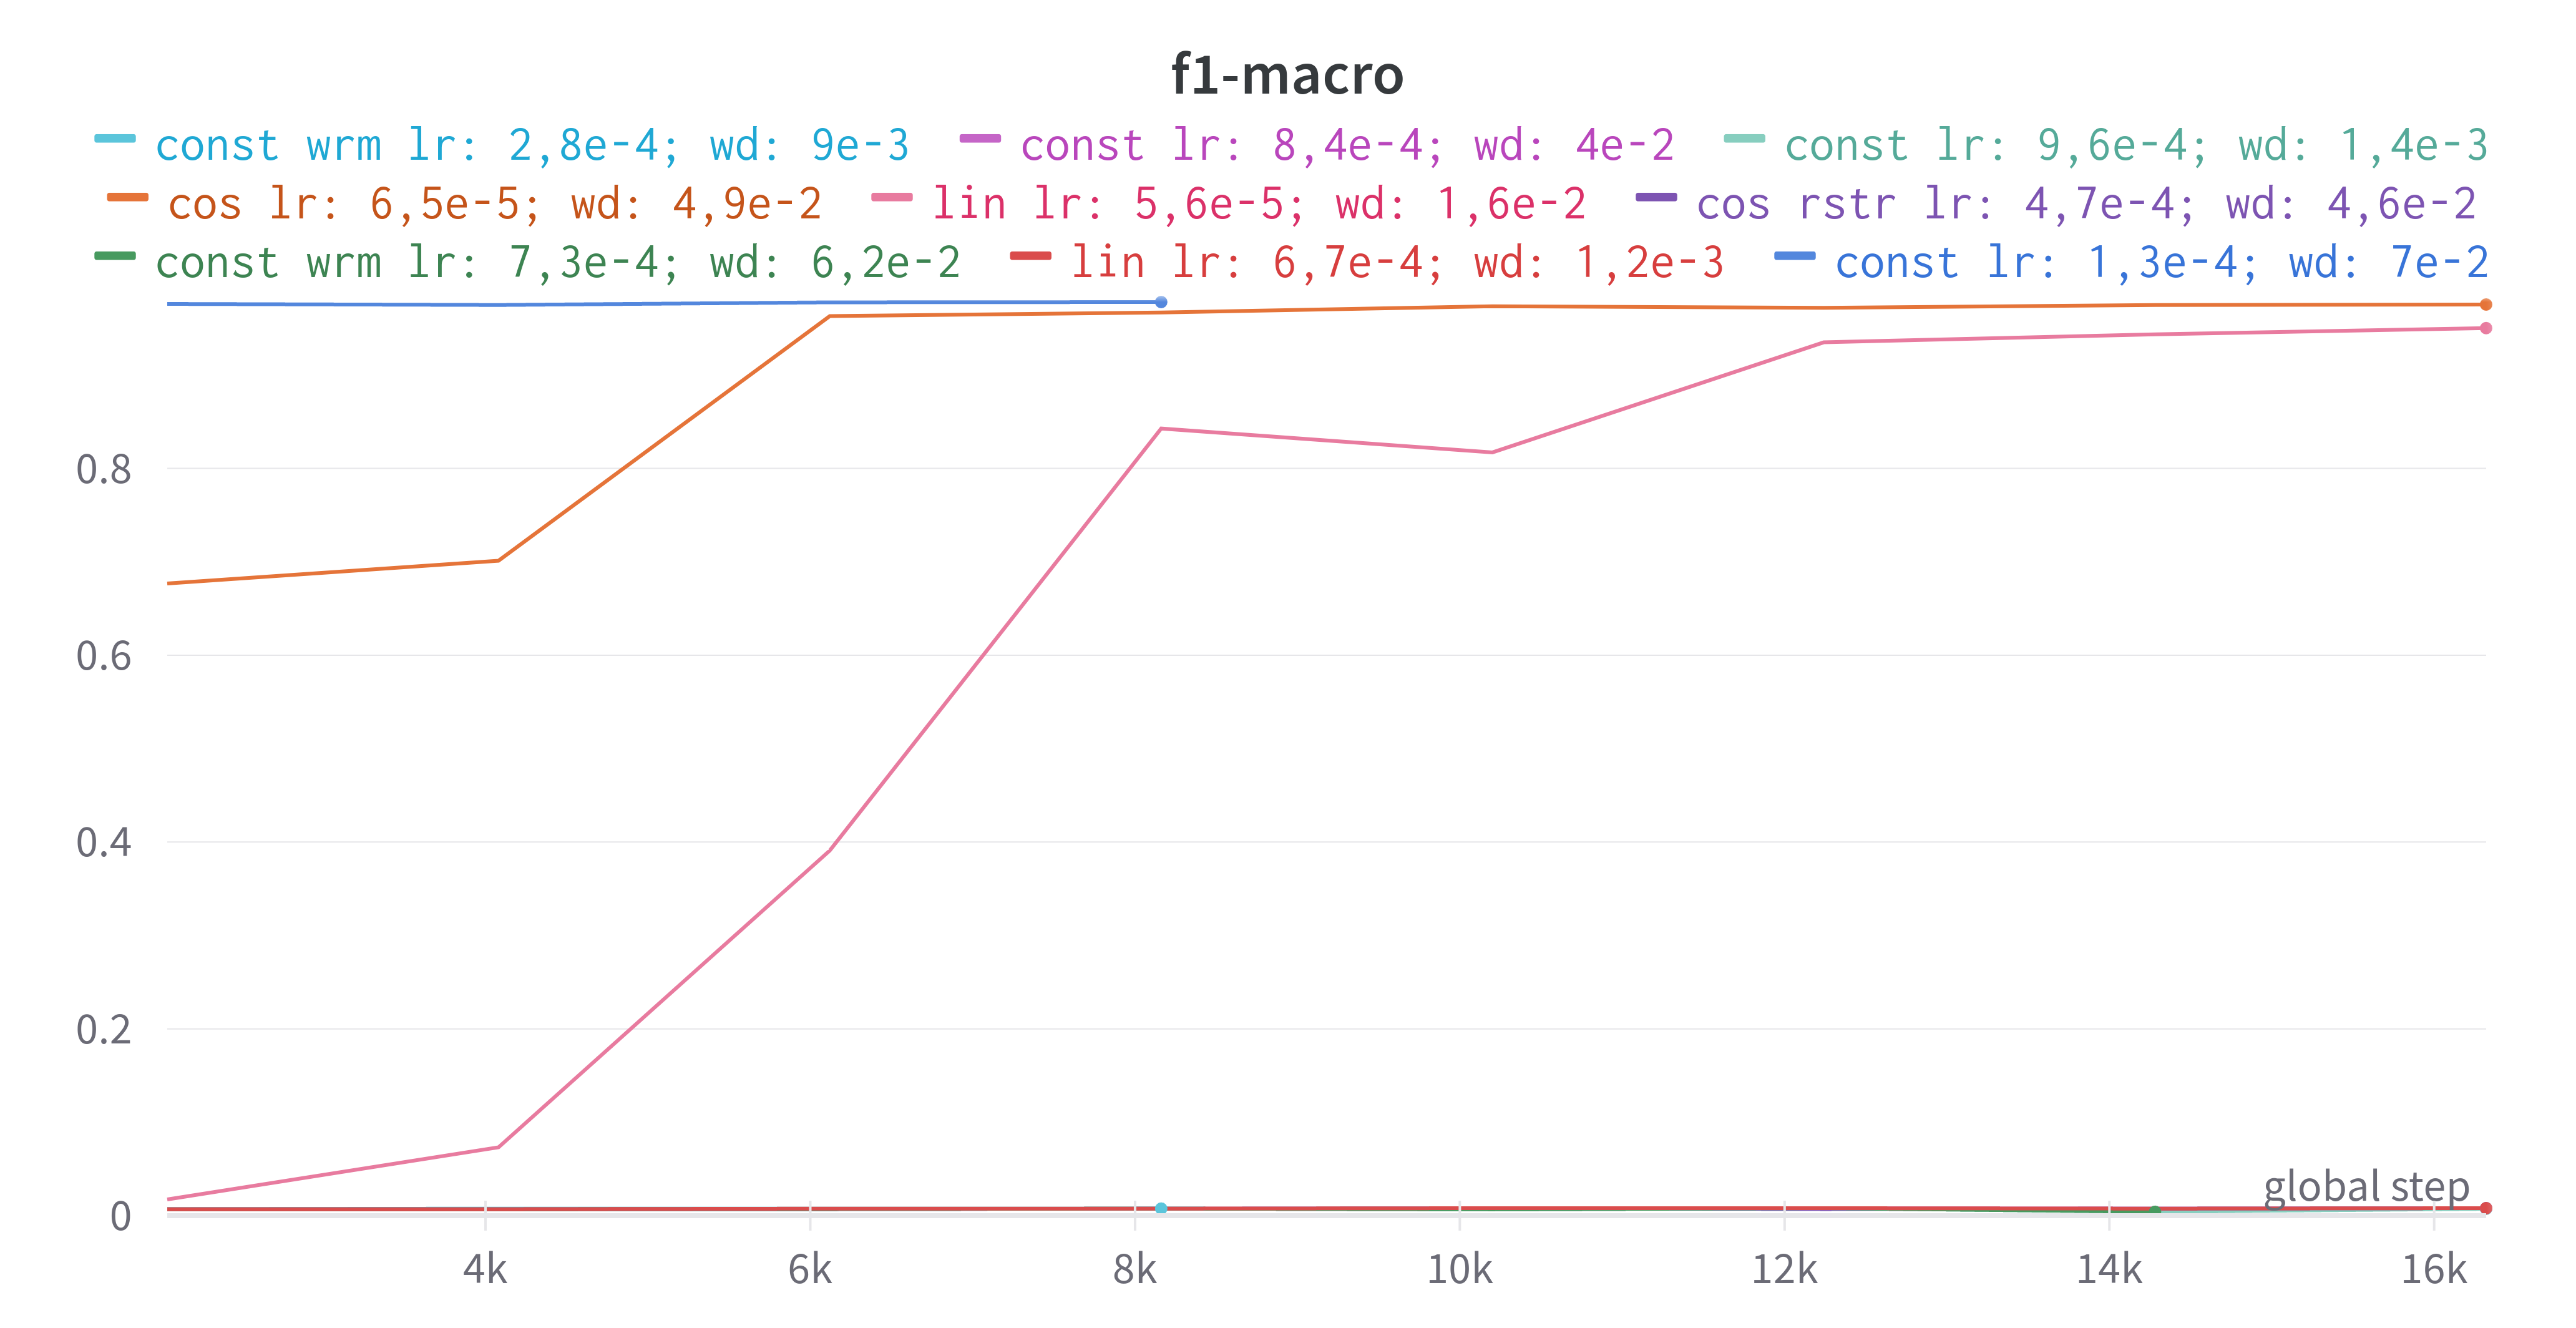
\includegraphics[width=\linewidth]{bert/f1-macro.png}
     \caption{Macro $F_1$ во время обучения BERT} 
   \end{minipage} 
\end{figure}

\begin{figure}[!htb] 
   \begin{minipage}{0.48\textwidth} 
     \centering 
     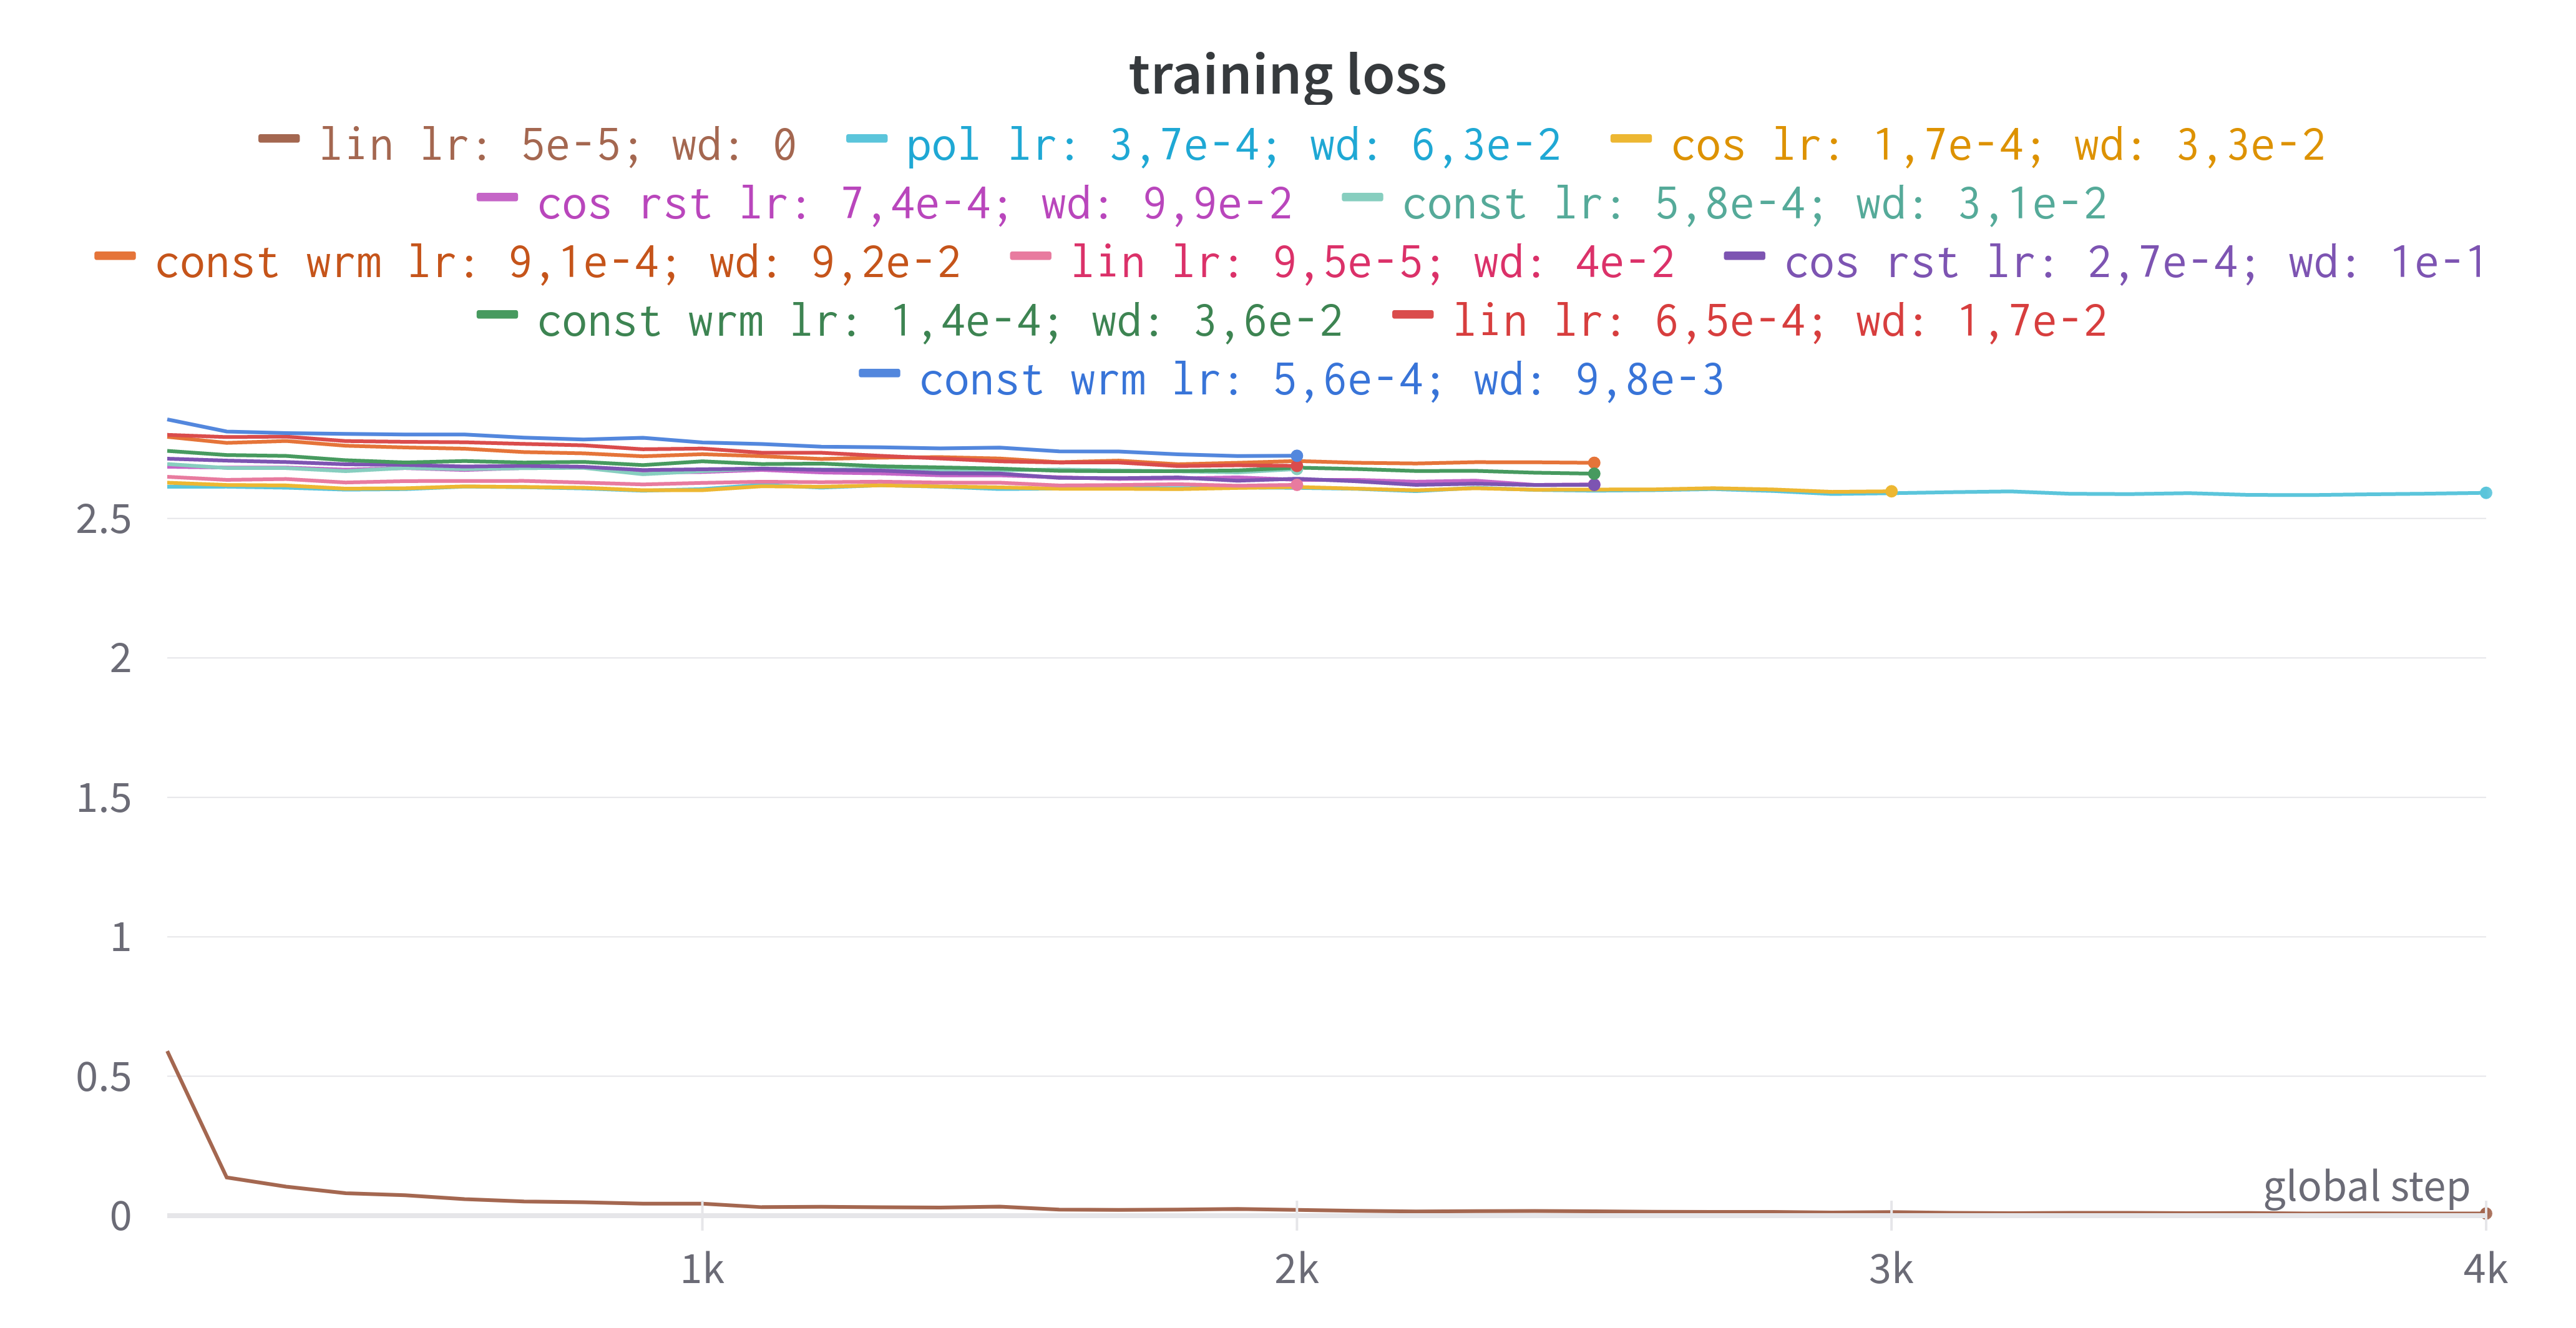
\includegraphics[width=\linewidth]{roberta/train-loss.png}
     \caption{График функции ошибки во время обучения RoBERTa} 
   \end{minipage}\hfill 
   \begin{minipage}{0.48\textwidth} 
     \centering 
     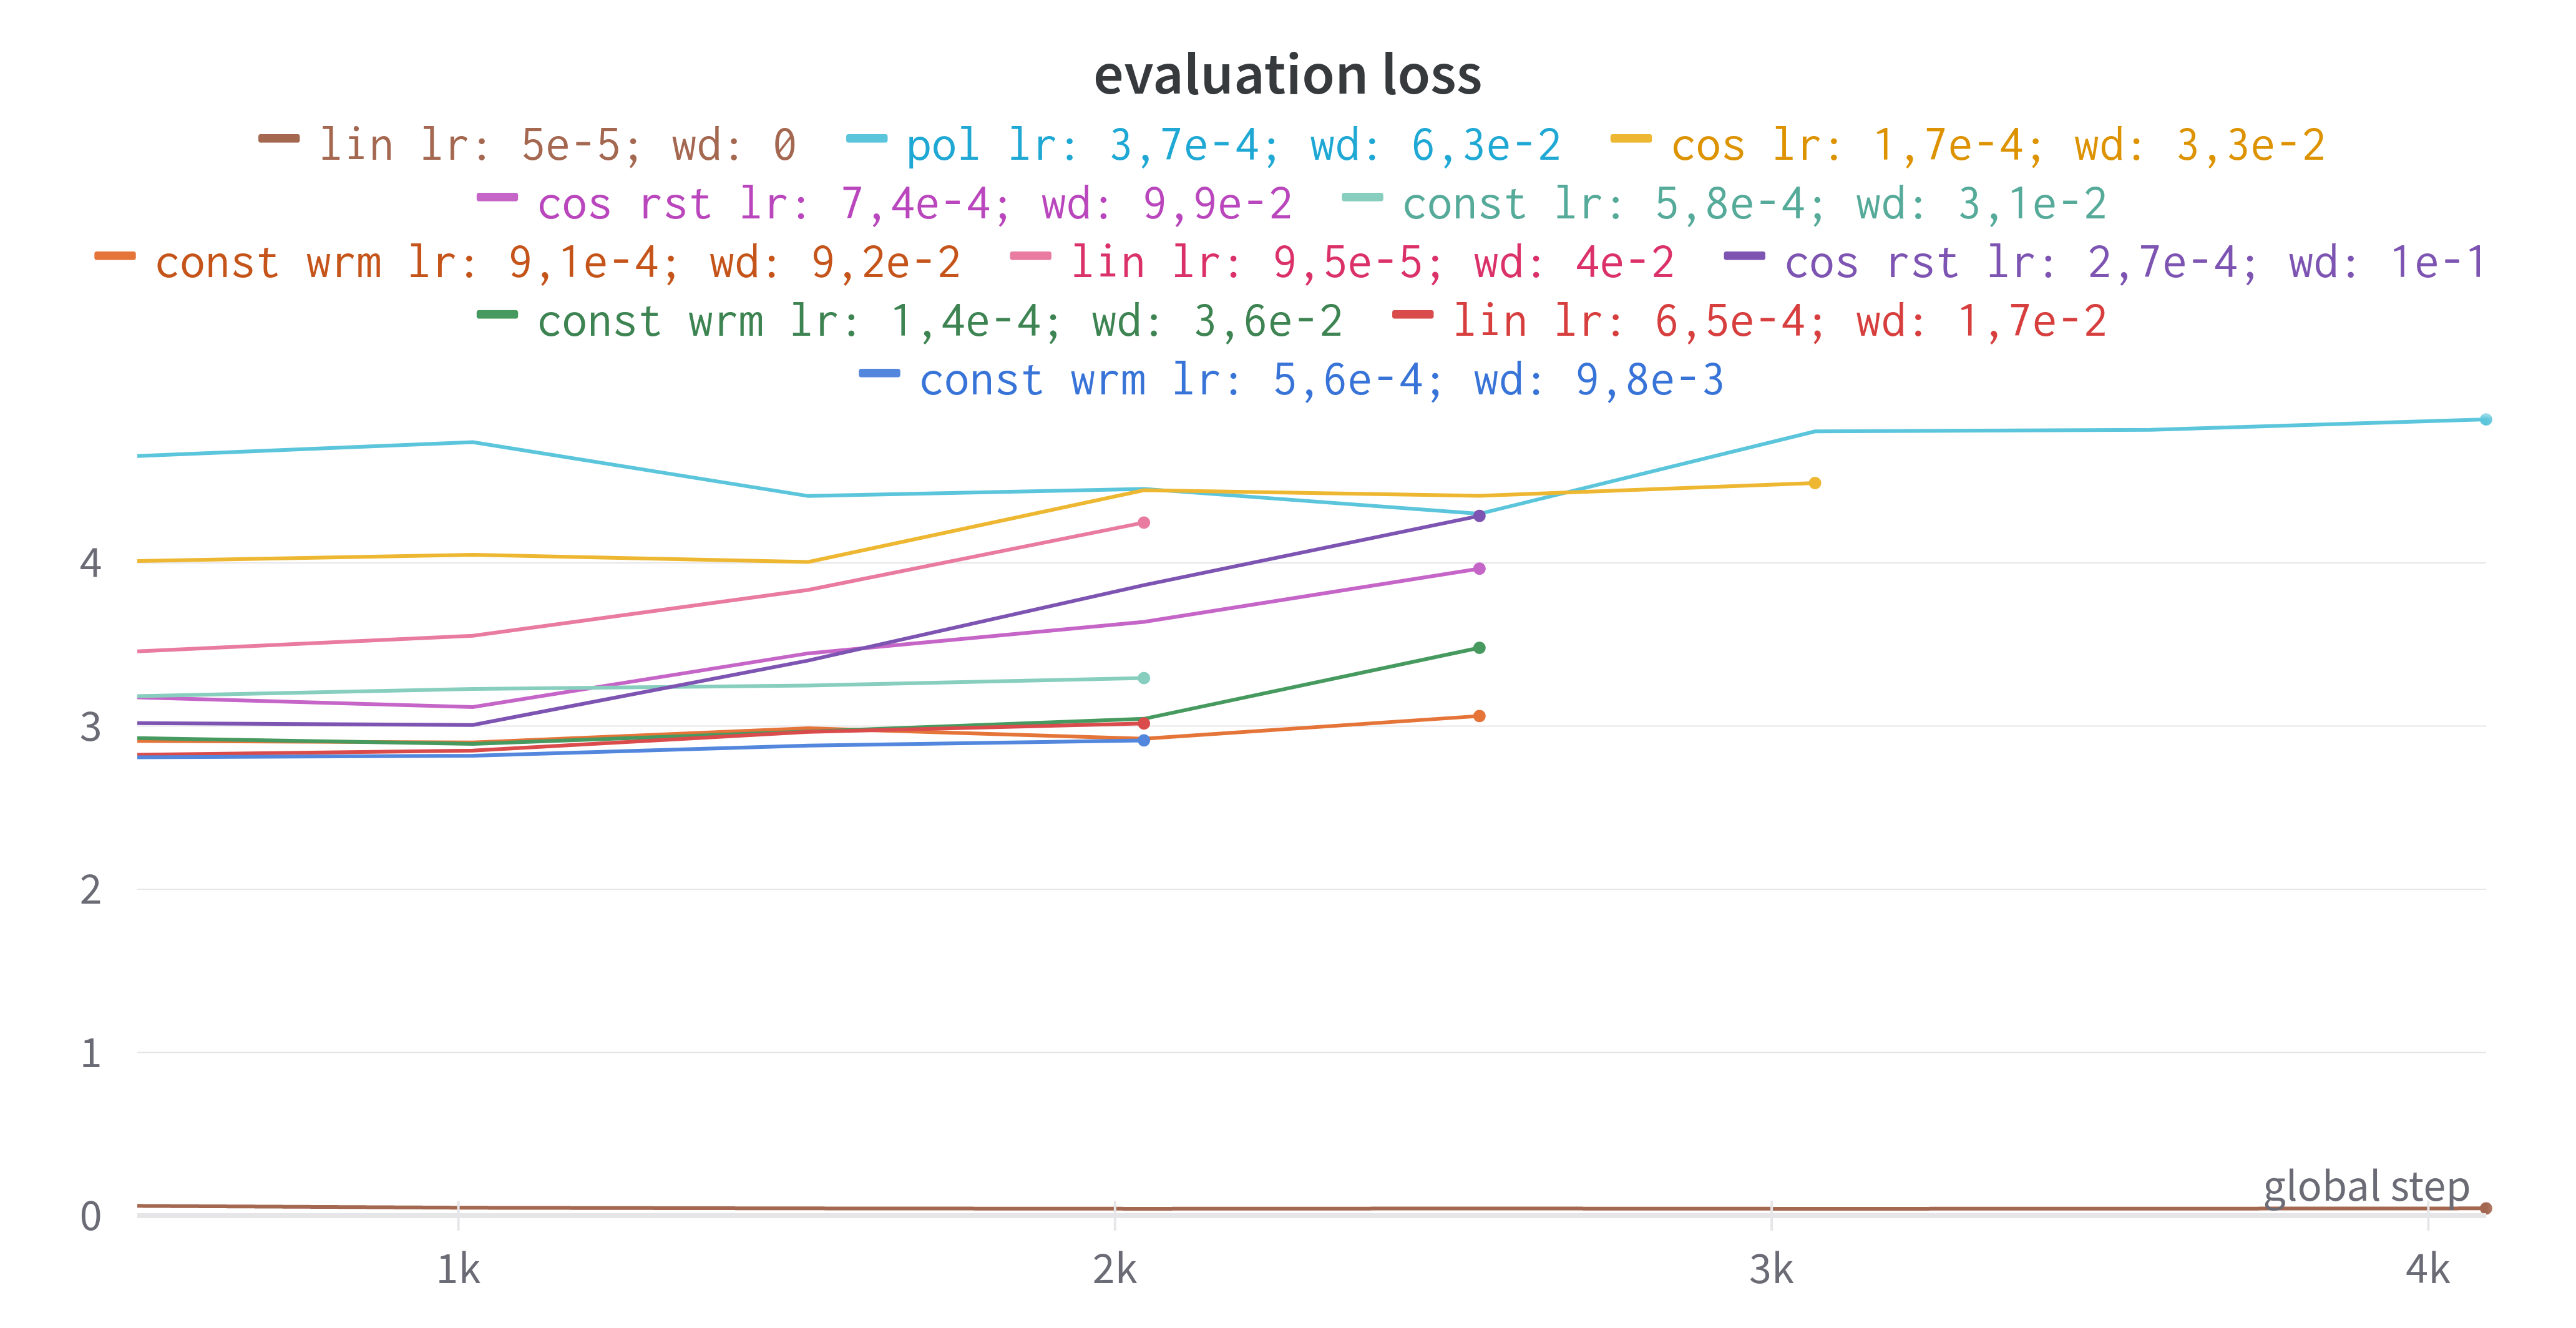
\includegraphics[width=\linewidth]{roberta/eval-loss.png}
     \caption{График функции ошибки при валидации RoBERTa} 
   \end{minipage} 
\end{figure}

\begin{figure}[!htb] 
   \begin{minipage}{0.48\textwidth} 
     \centering 
     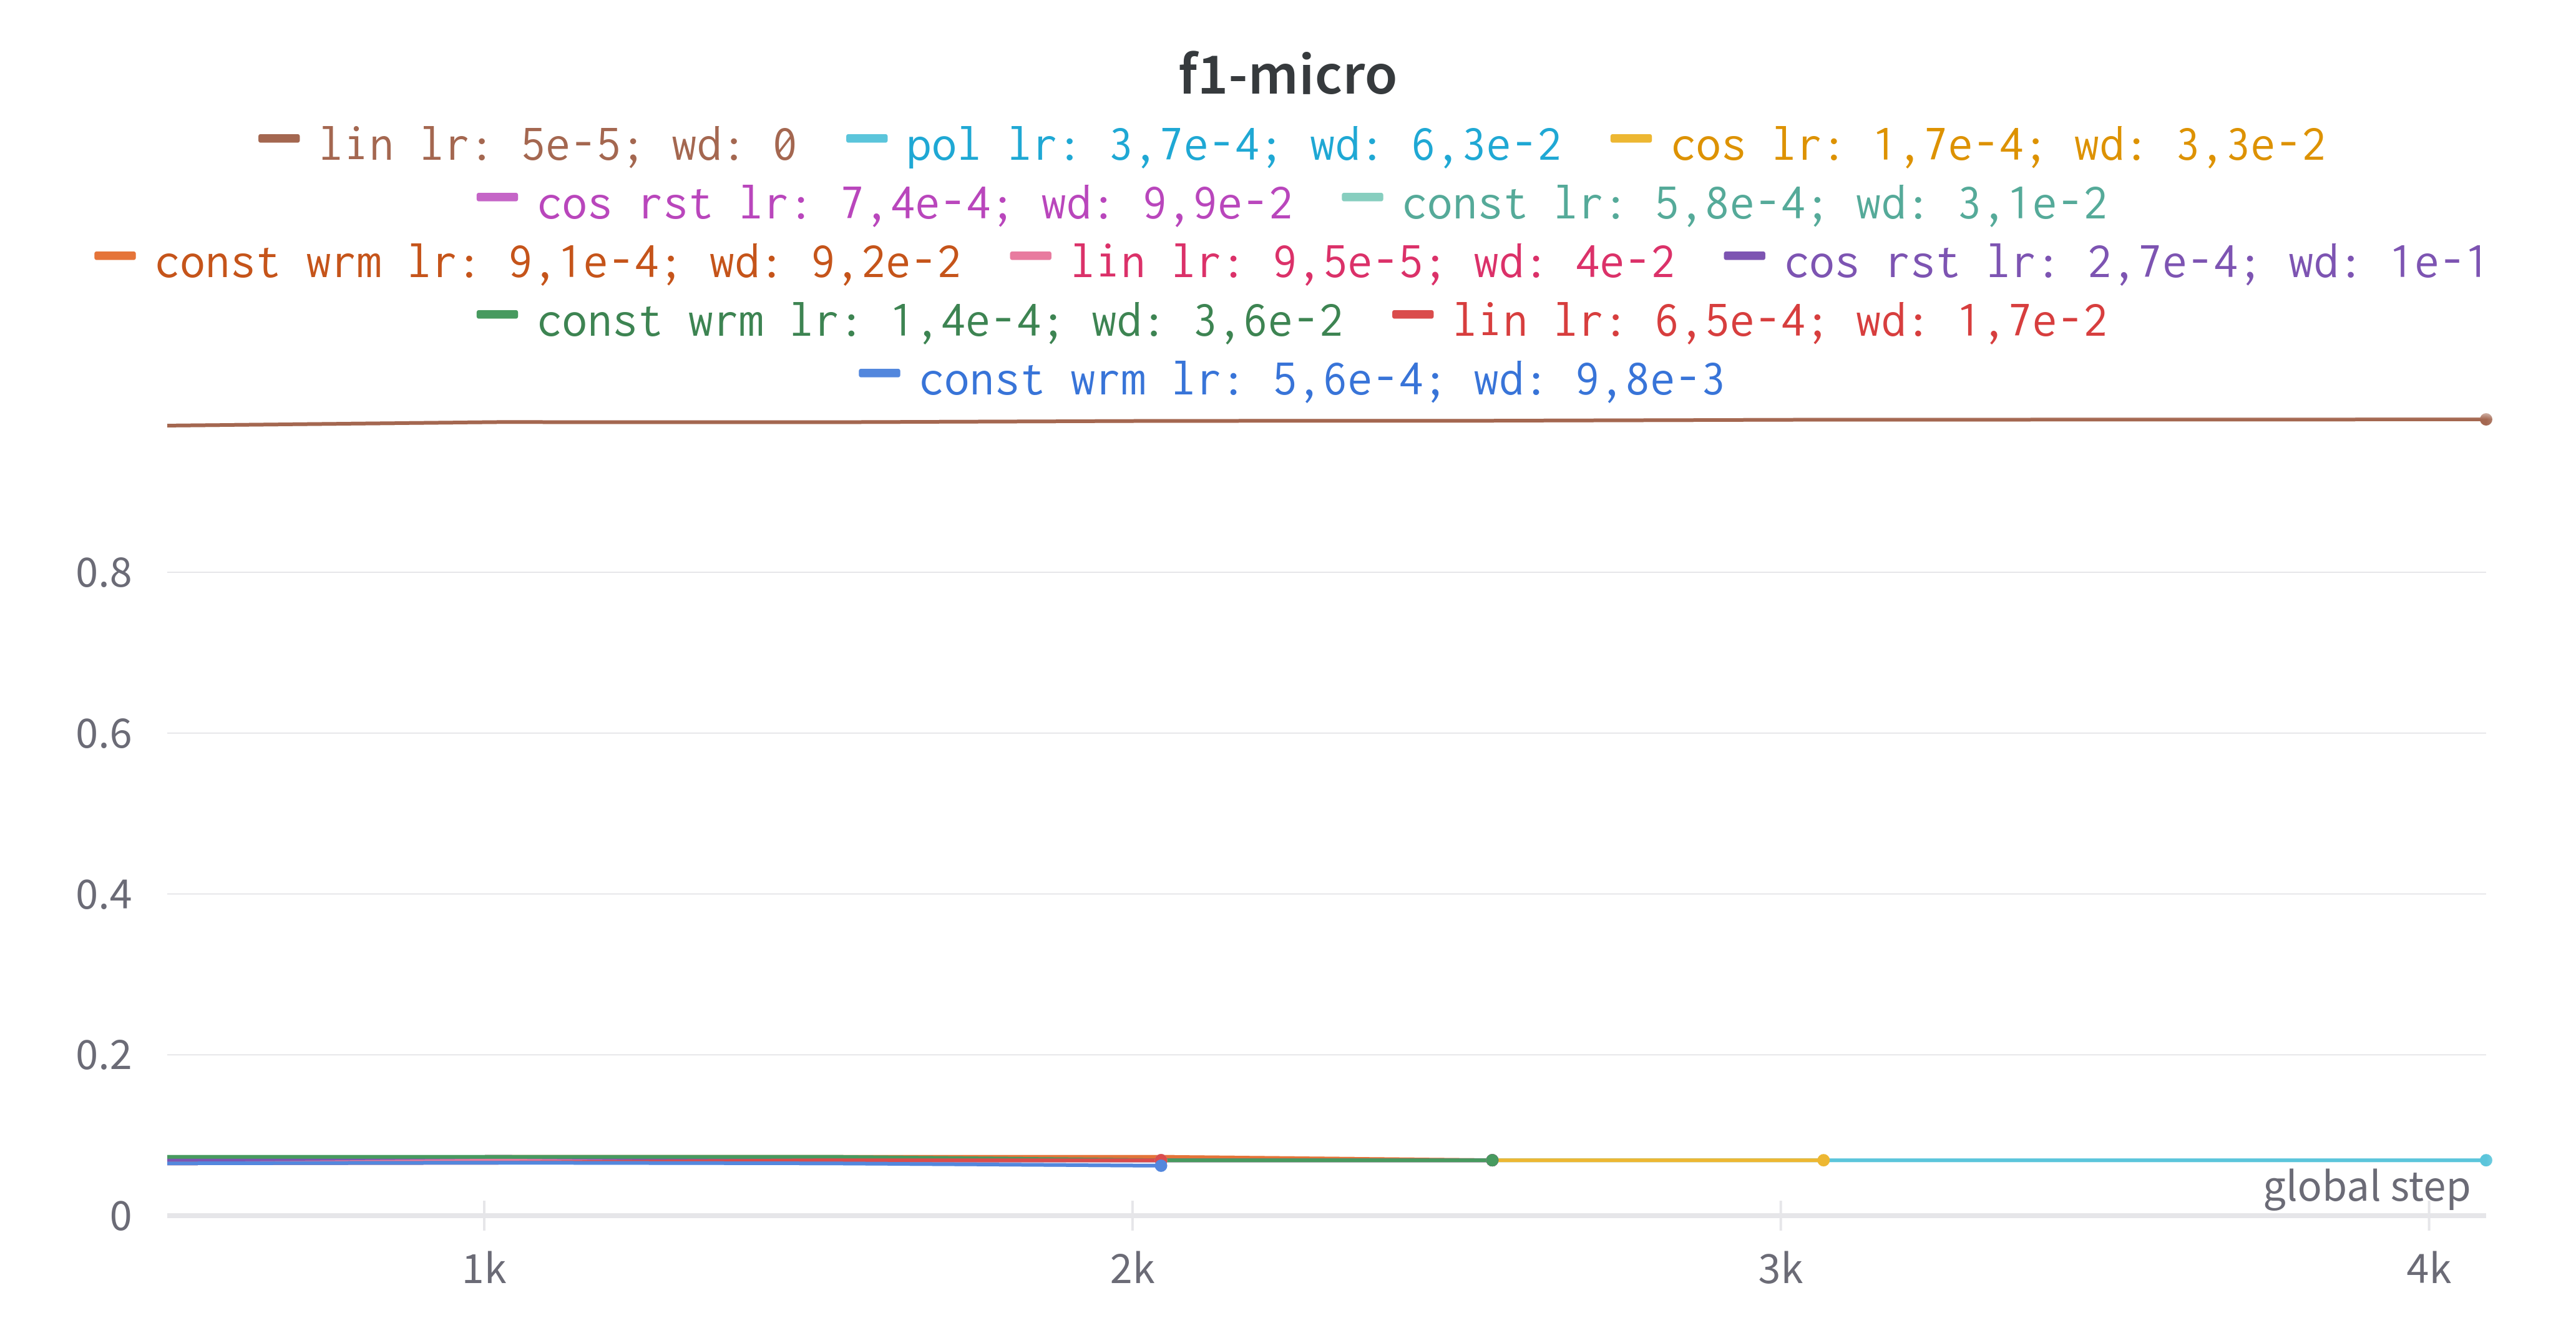
\includegraphics[width=\linewidth]{roberta/f1-micro.png}
     \caption{Micro $F_1$ во время обучения RoBERTa} 
   \end{minipage}\hfill 
   \begin{minipage}{0.48\textwidth} 
     \centering 
     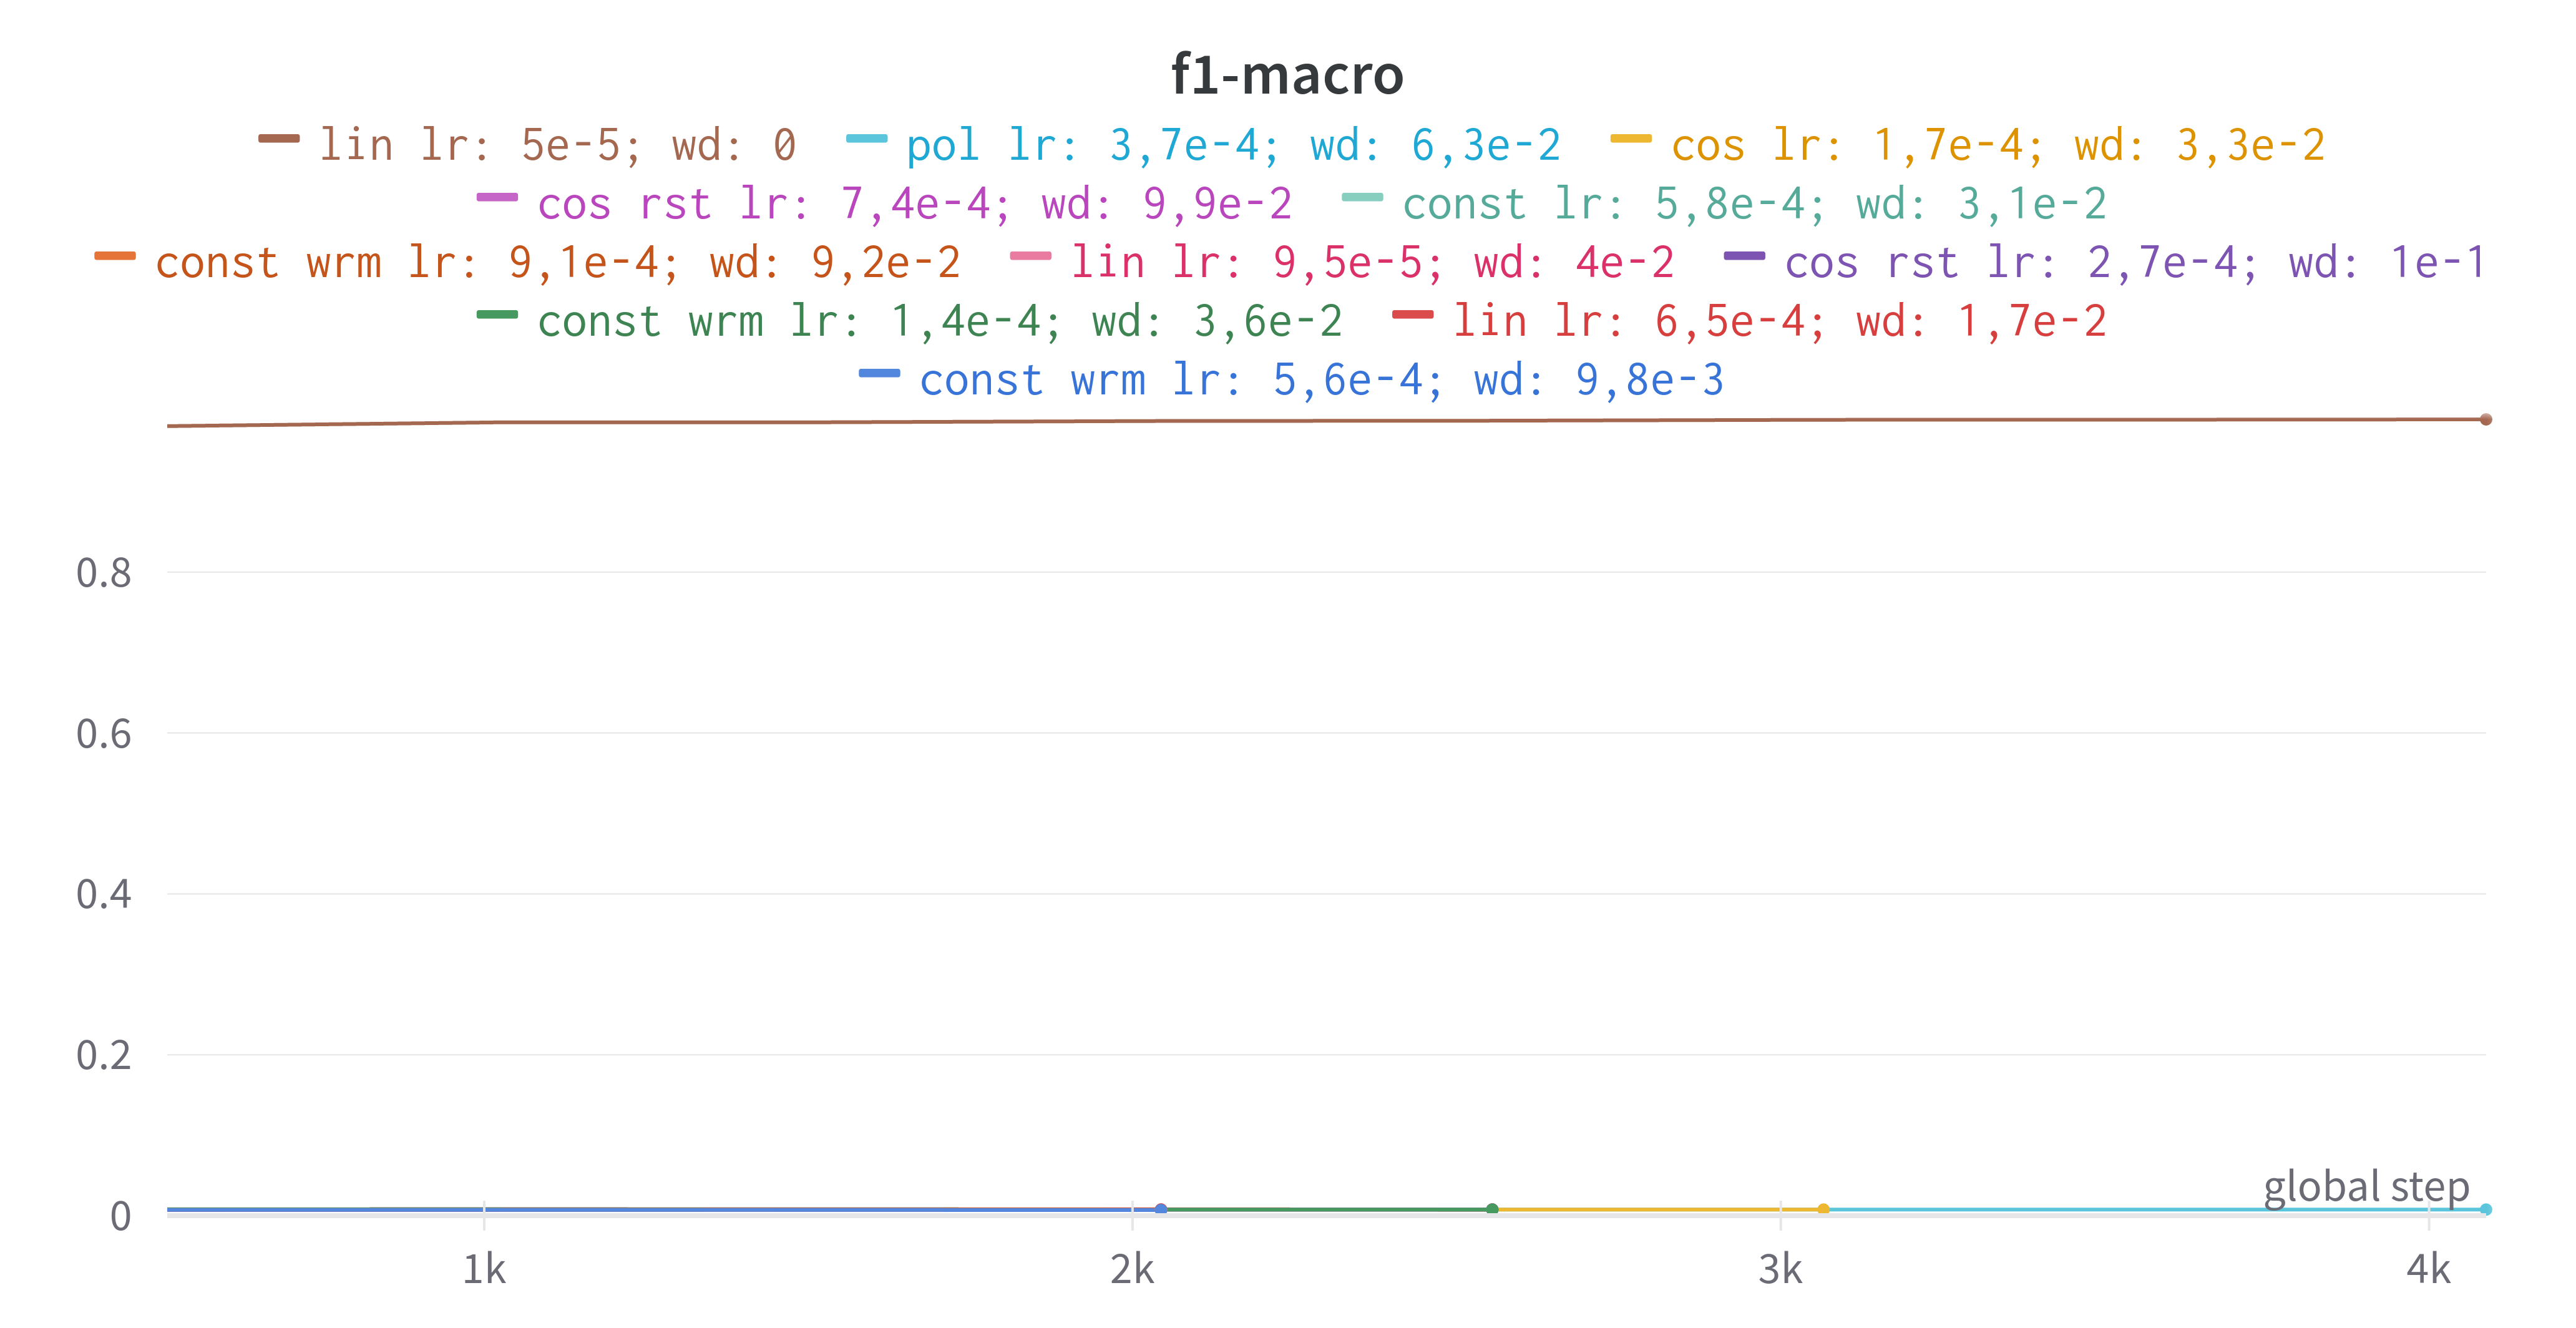
\includegraphics[width=\linewidth]{roberta/f1-macro.png}
     \caption{Macro $F_1$ во время обучения RoBERTa} 
   \end{minipage} 
\end{figure}

\begin{figure}[!htb] 
   \begin{minipage}{0.48\textwidth} 
     \centering 
     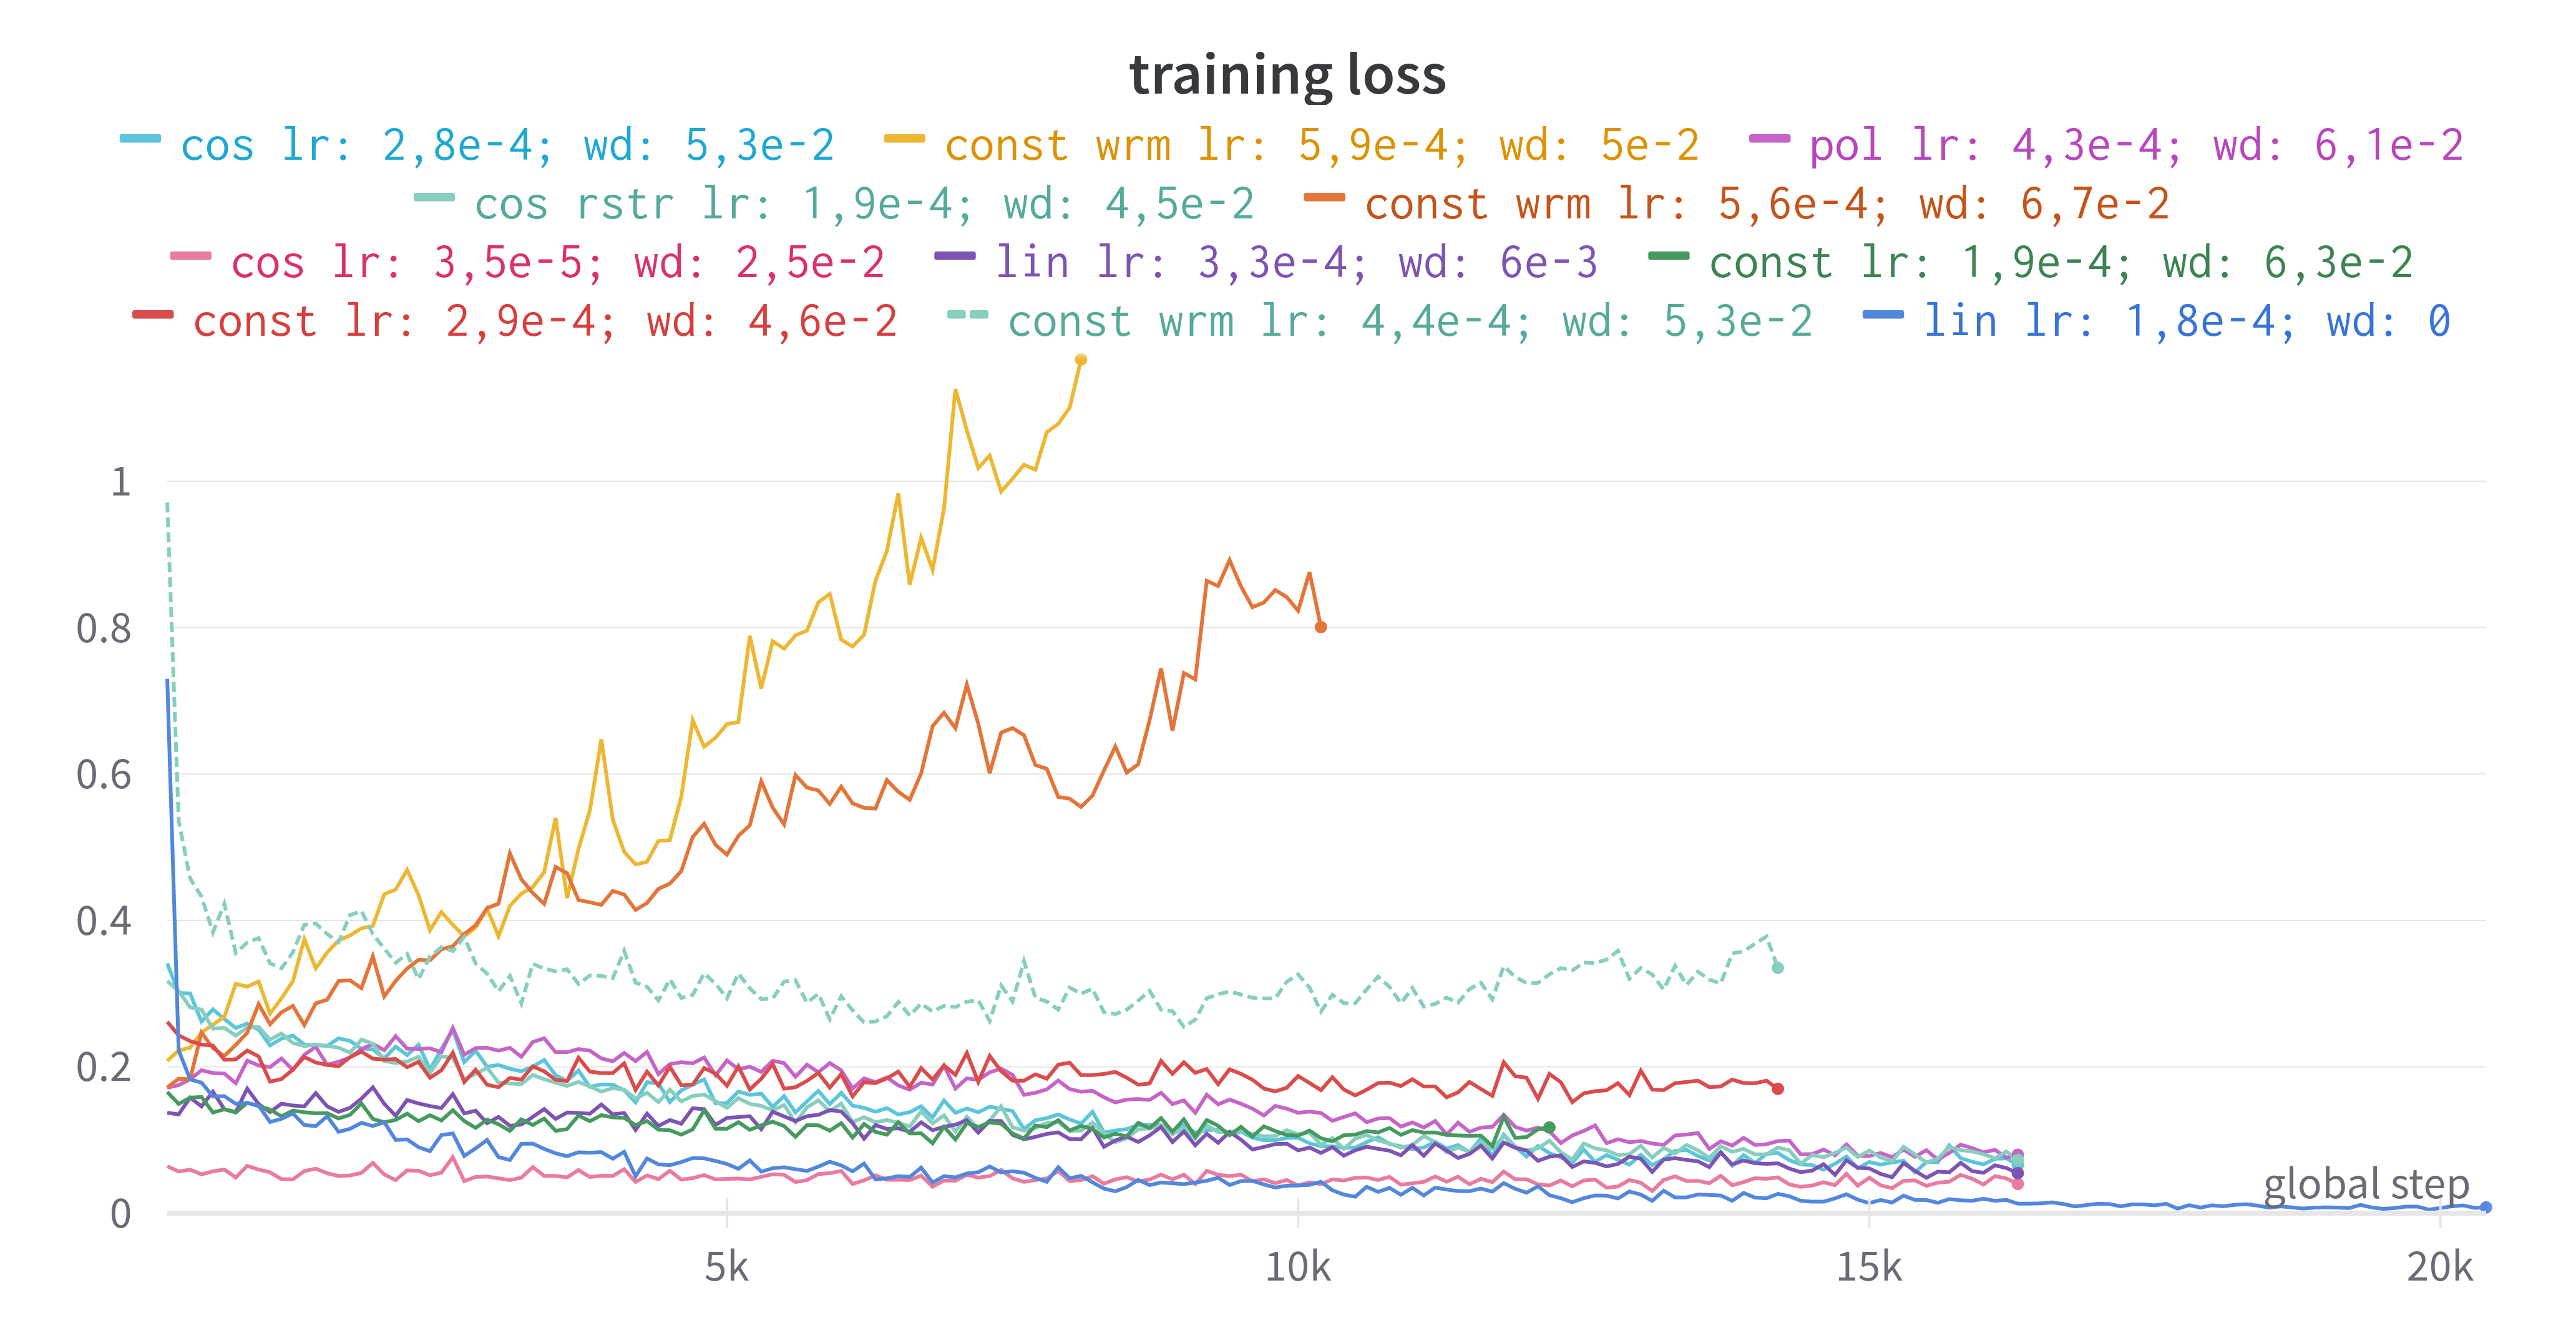
\includegraphics[width=\linewidth]{distilbert/train-loss.png}
     \caption{График функции ошибки во время обучения DistilBERT} 
   \end{minipage}\hfill 
   \begin{minipage}{0.48\textwidth} 
     \centering 
     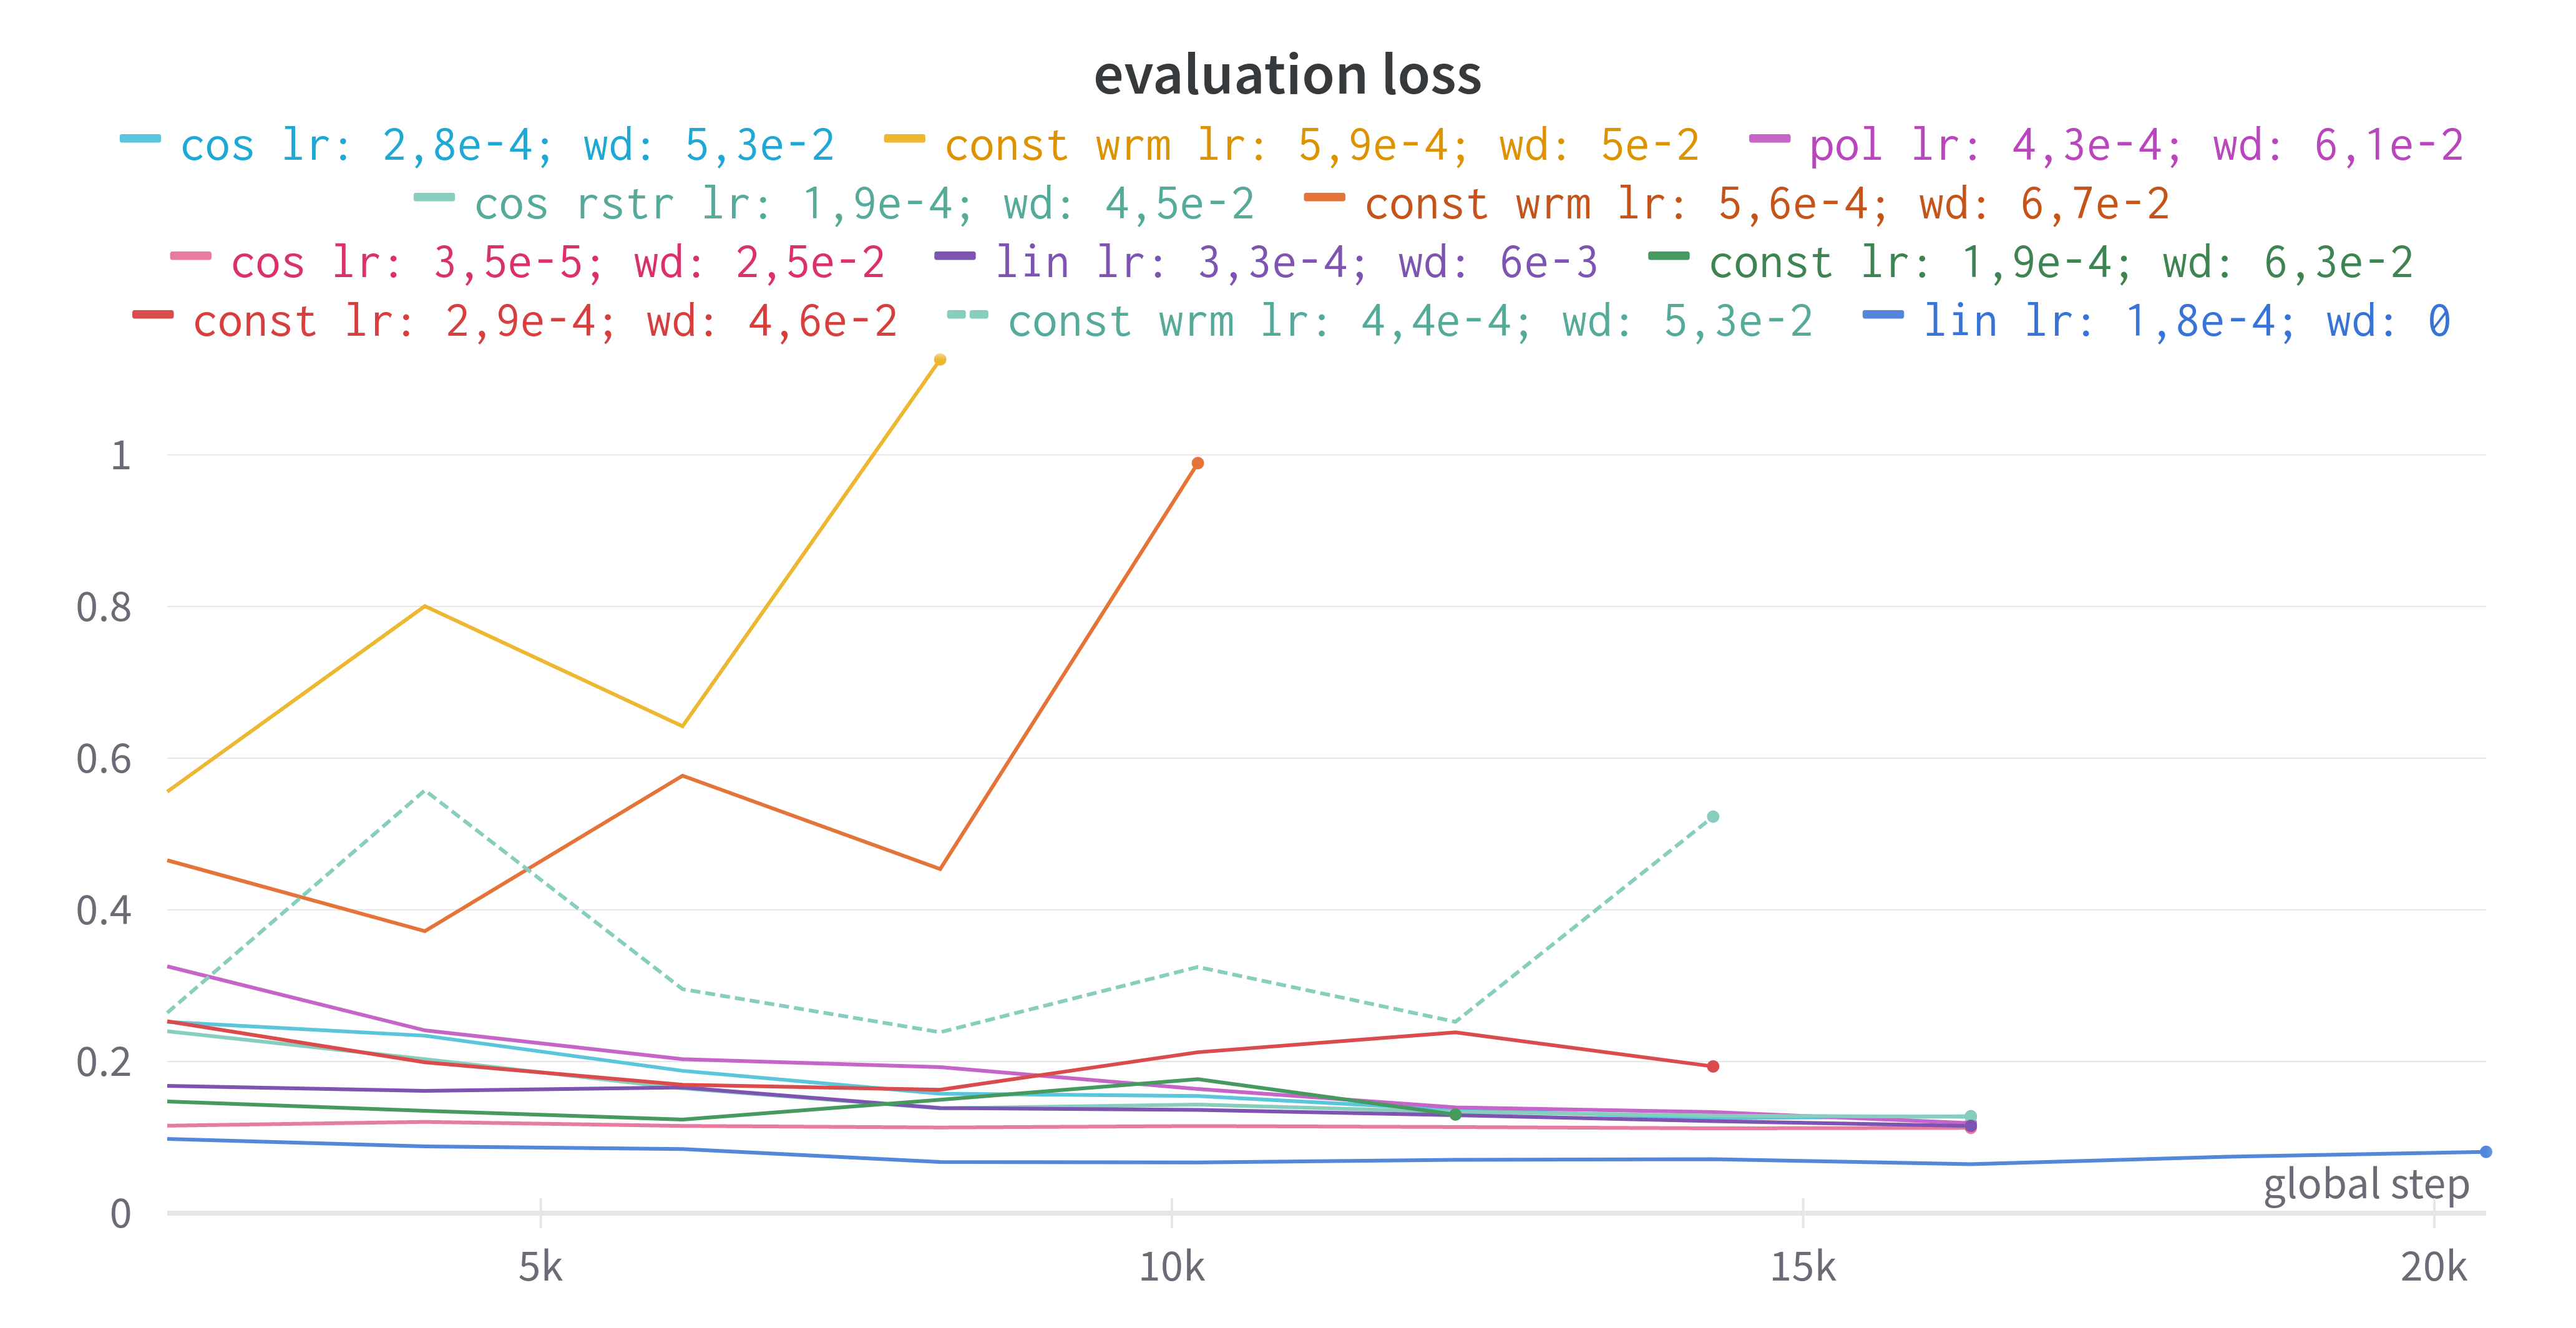
\includegraphics[width=\linewidth]{distilbert/eval-loss.png}
     \caption{График функции ошибки при валидации DistilBERT} 
   \end{minipage} 
\end{figure}

\begin{figure}[!htb] 
   \begin{minipage}{0.48\textwidth} 
     \centering 
     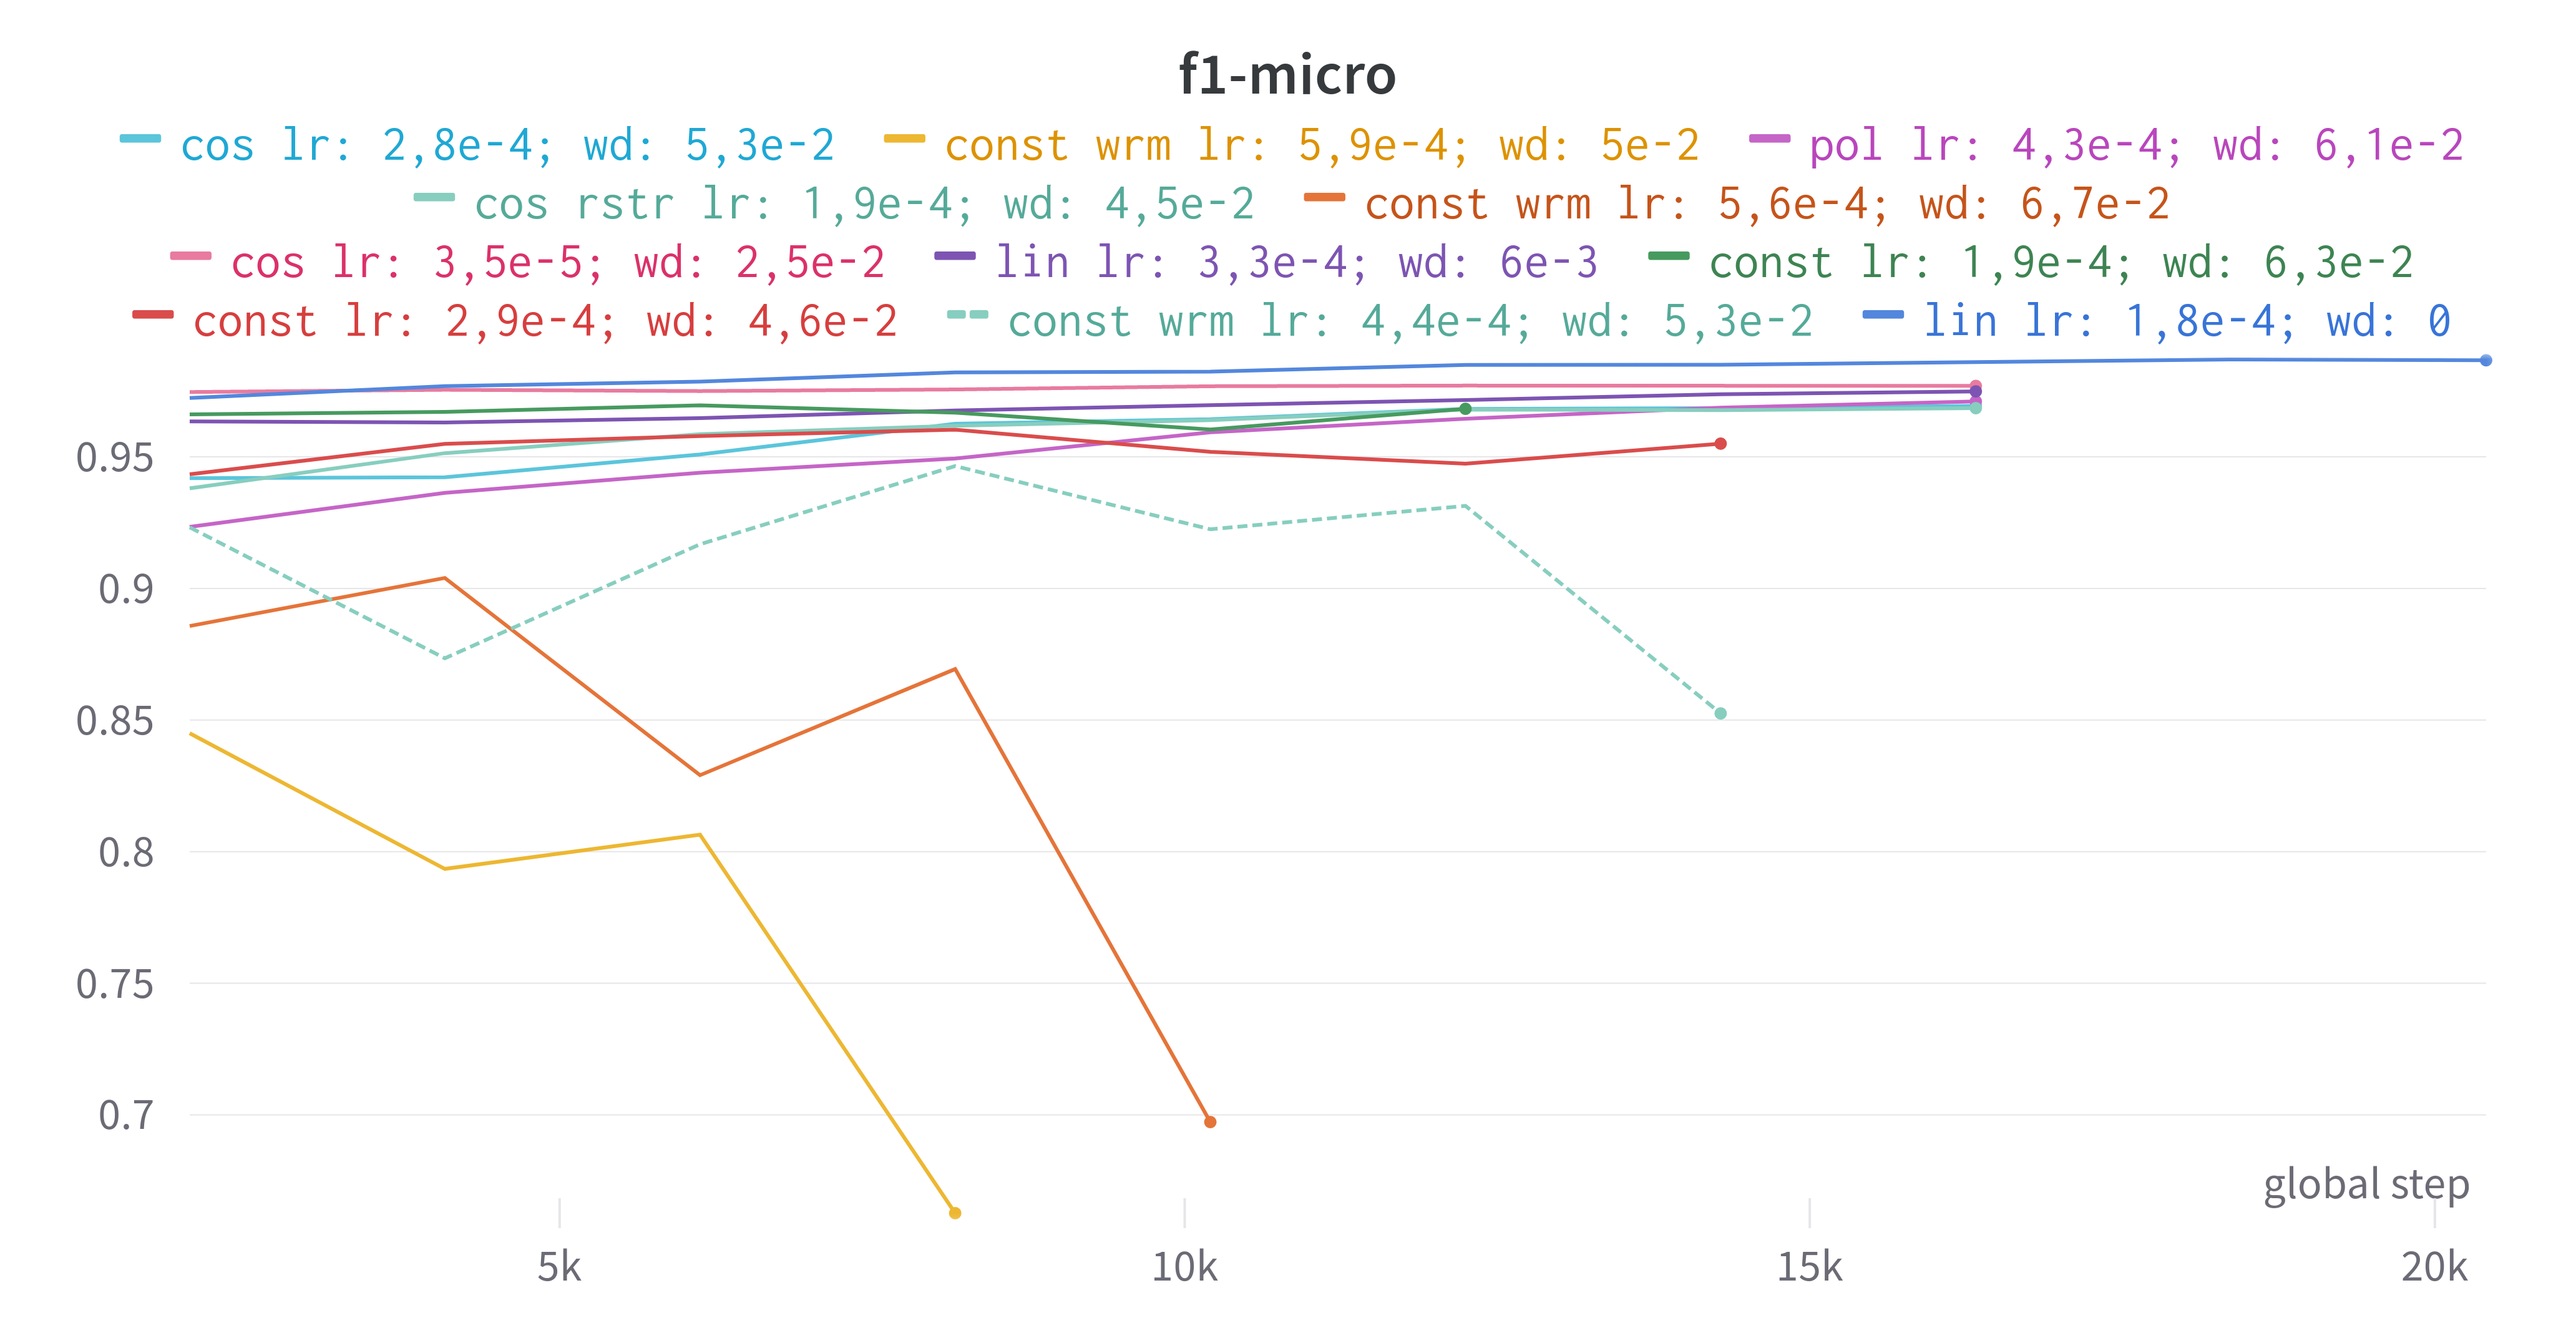
\includegraphics[width=\linewidth]{distilbert/f1-micro.png}
     \caption{Micro $F_1$ во время обучения DistilBERT} 
   \end{minipage}\hfill 
   \begin{minipage}{0.48\textwidth} 
     \centering 
     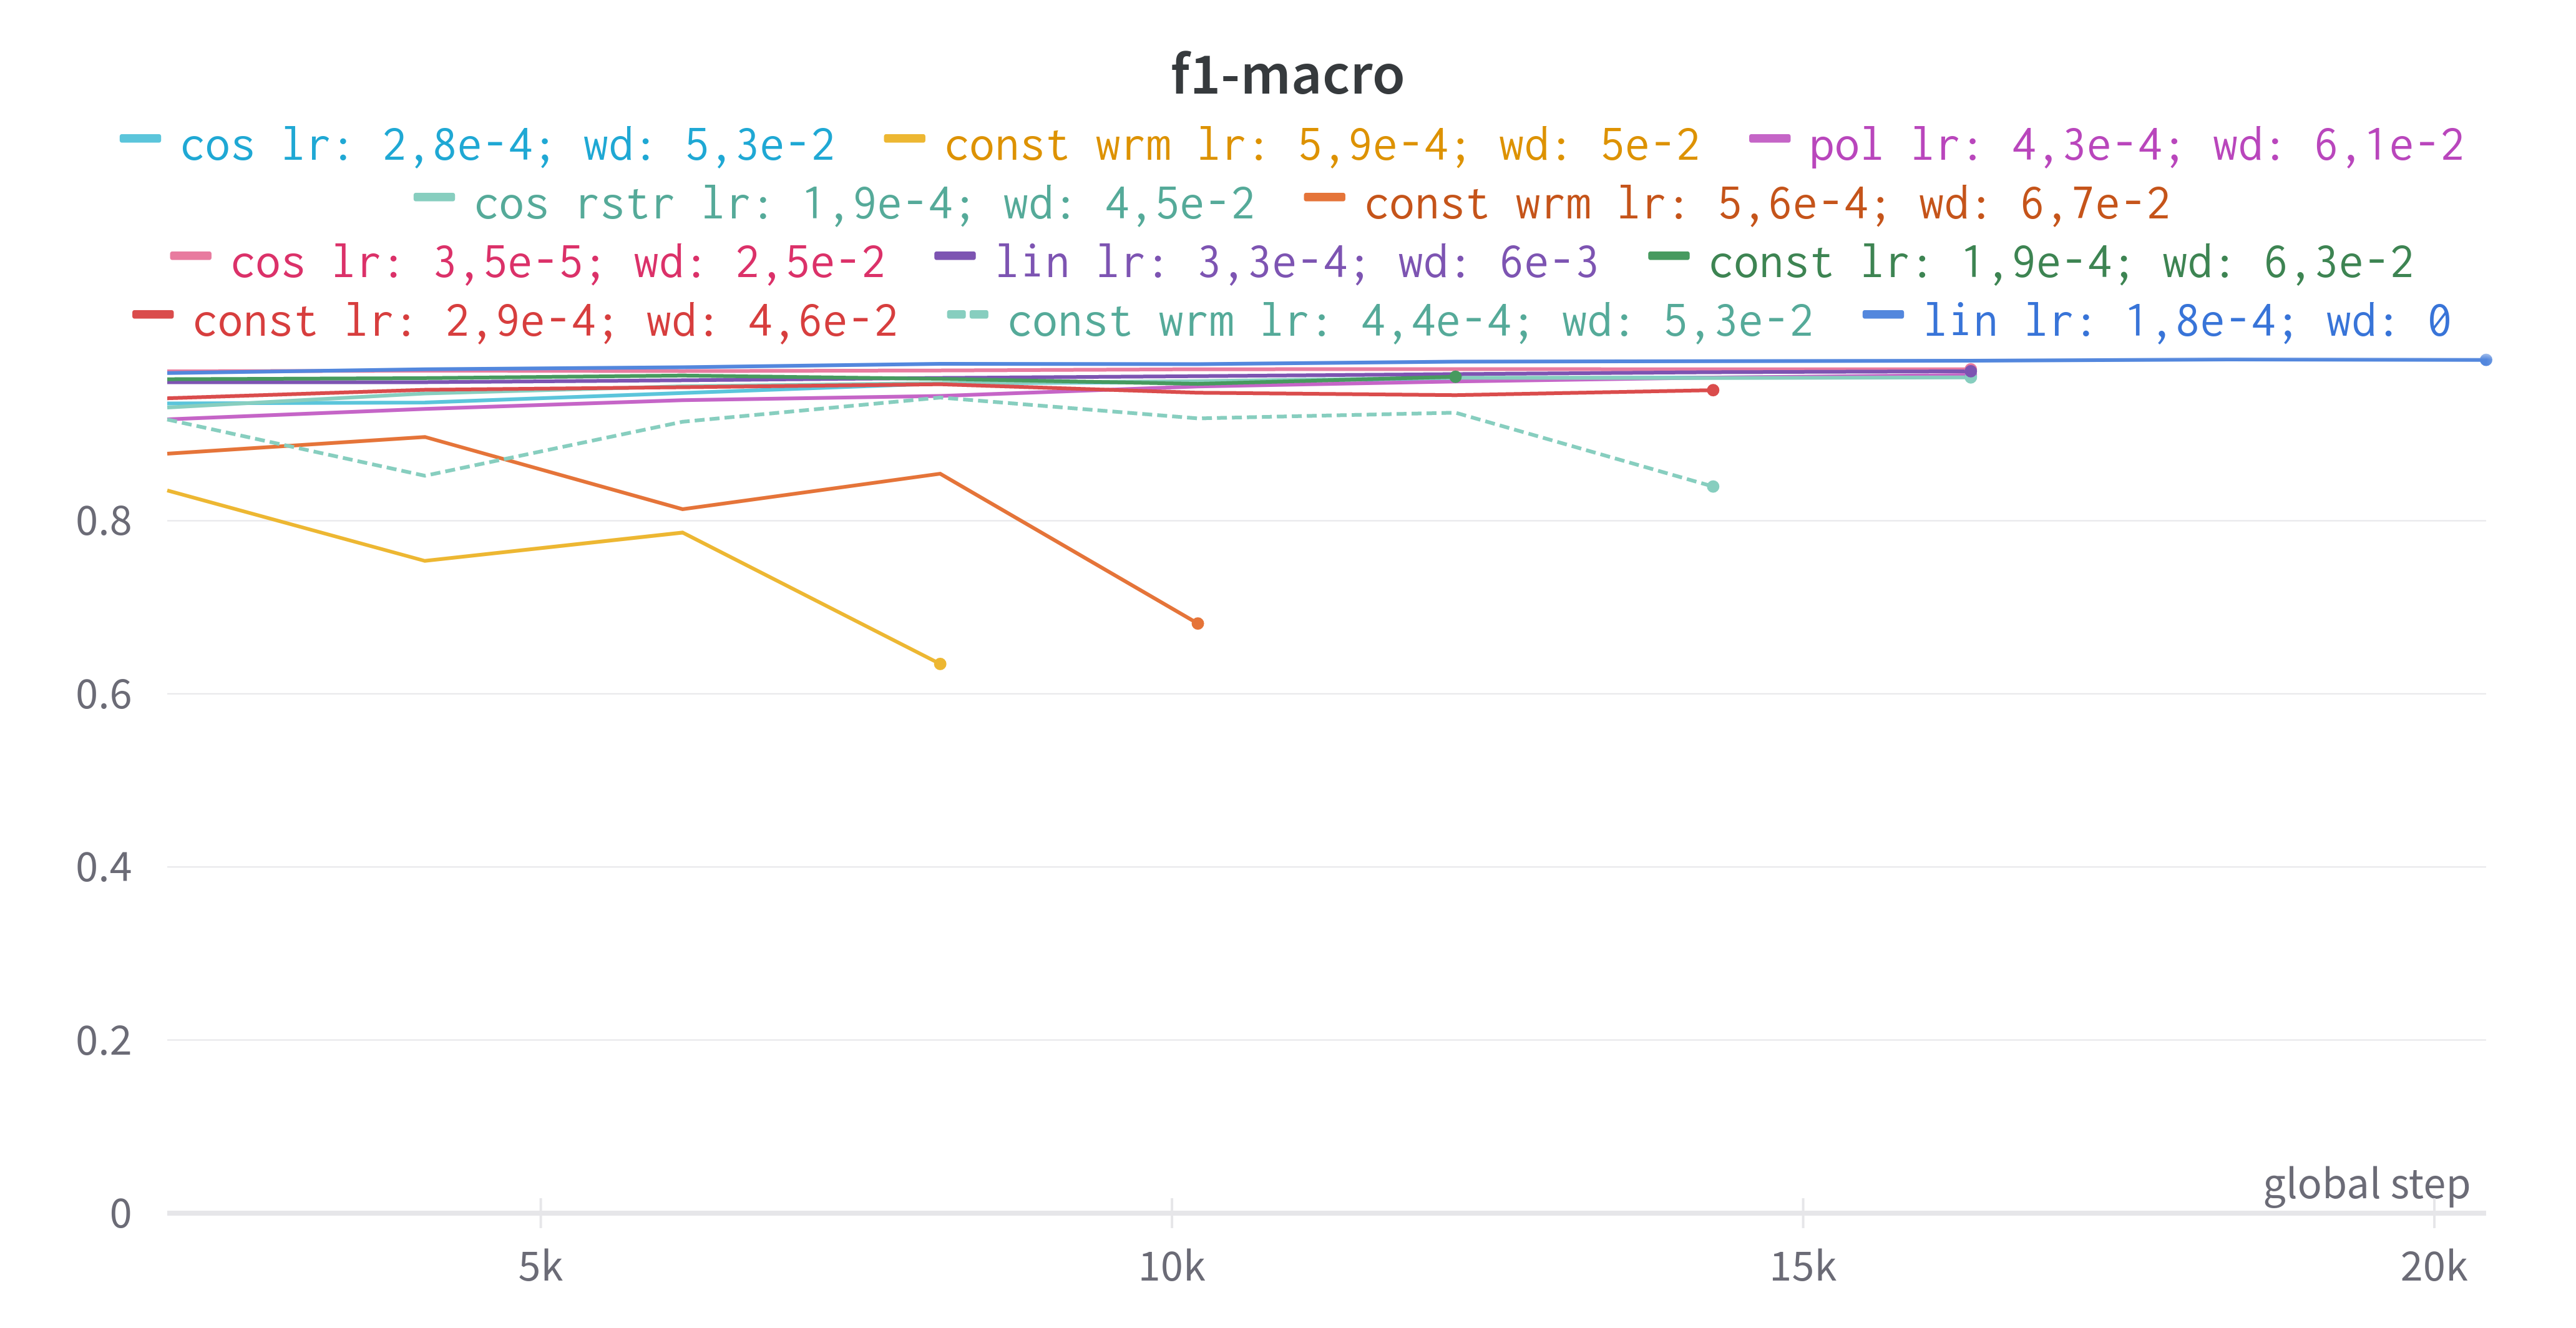
\includegraphics[width=\linewidth]{distilbert/f1-macro.png}
     \caption{Macro $F_1$ во время обучения DistilBERT} 
   \end{minipage} 
\end{figure}

\begin{figure}[!htb] 
   \begin{minipage}{0.48\textwidth} 
     \centering 
     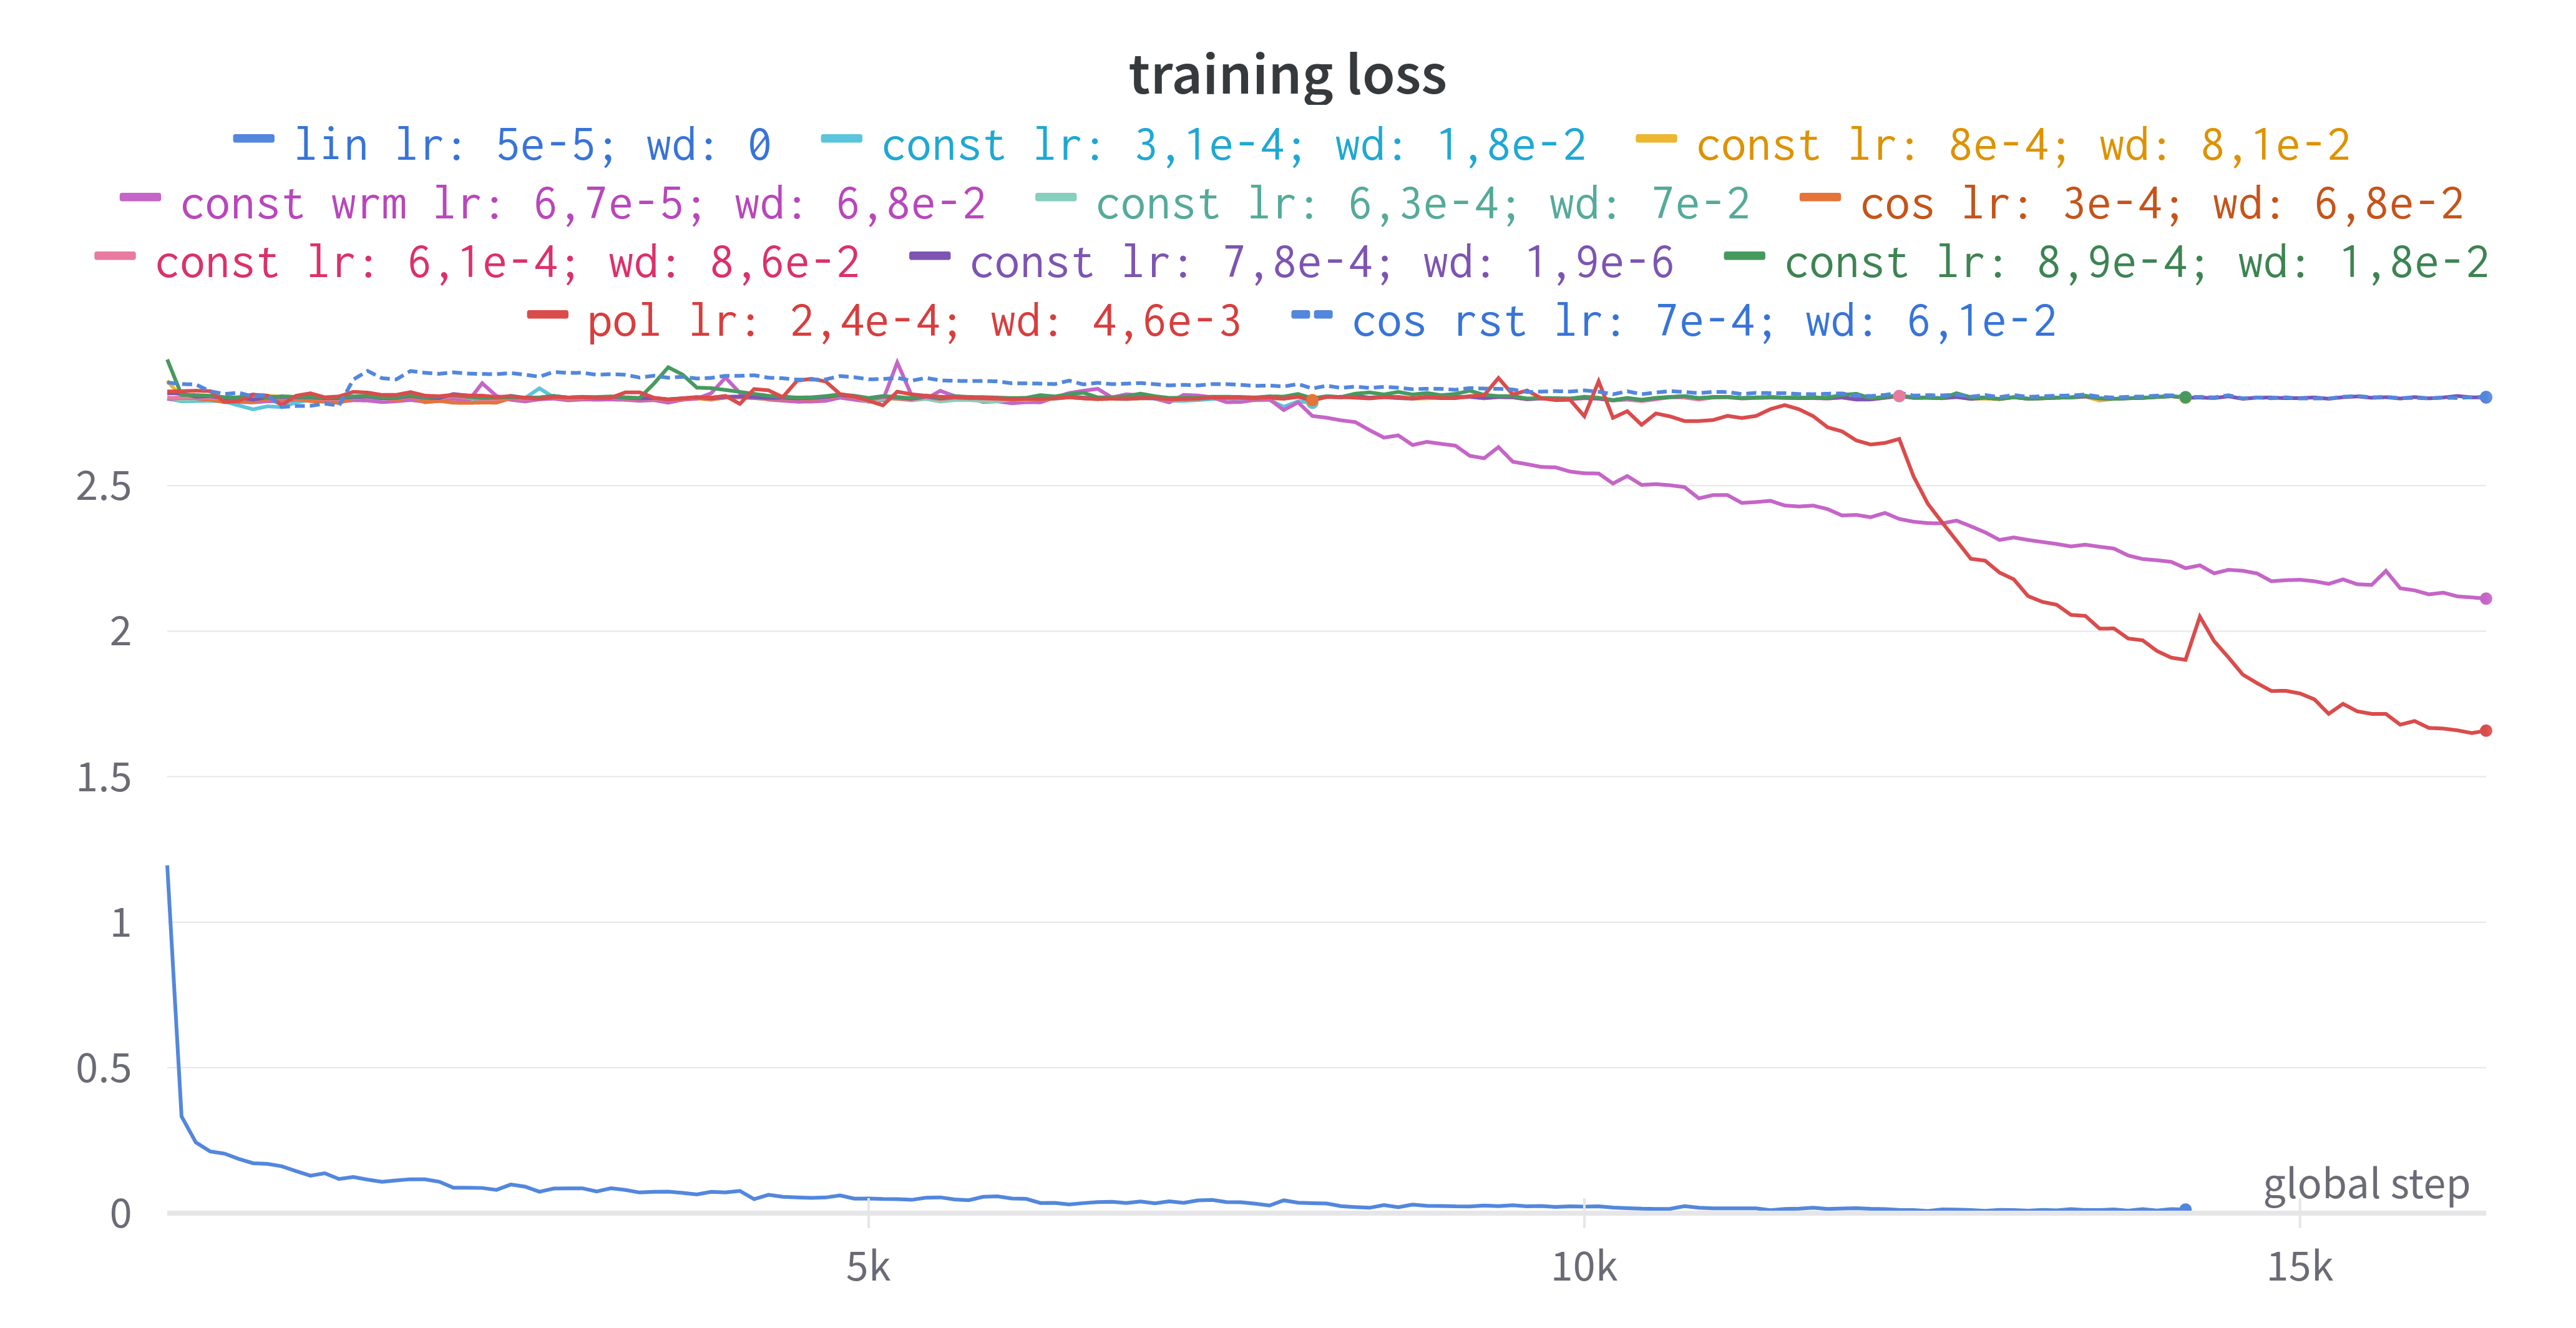
\includegraphics[width=\linewidth]{albert/train-loss.png}
     \caption{График функции ошибки во время обучения ALBERT} 
   \end{minipage}\hfill 
   \begin{minipage}{0.48\textwidth} 
     \centering 
     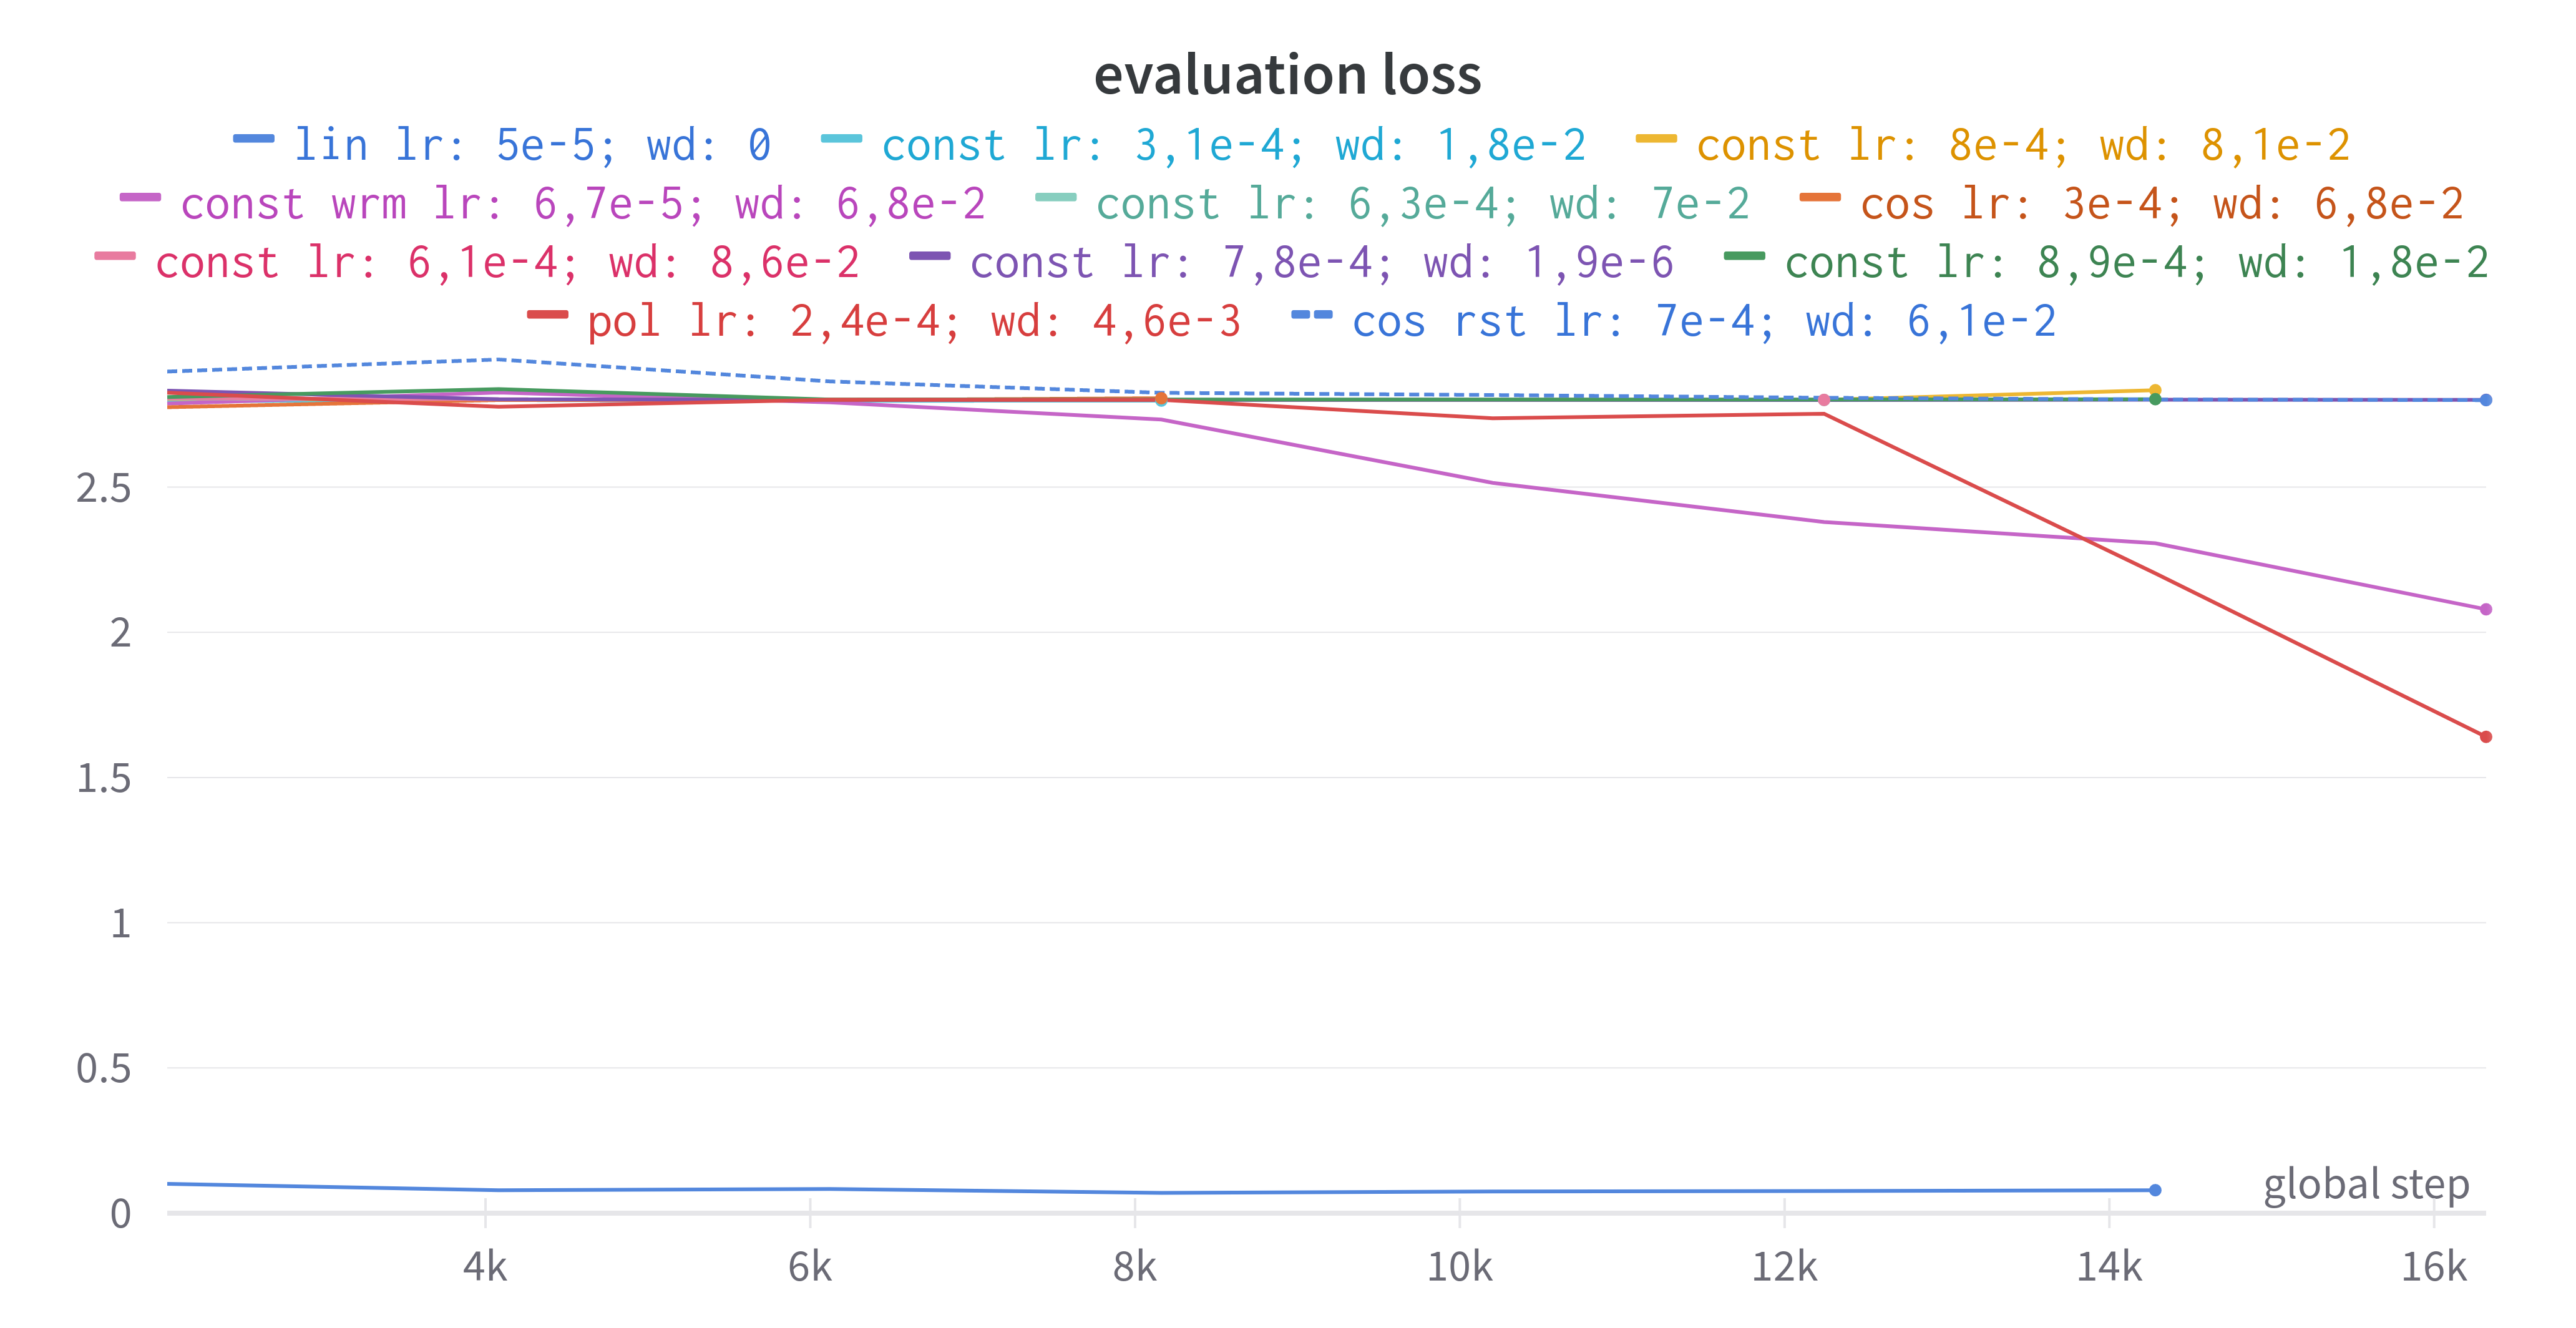
\includegraphics[width=\linewidth]{albert/eval-loss.png}
     \caption{График функции ошибки при валидации ALBERT} 
   \end{minipage} 
\end{figure}

\begin{figure}[!htb] 
   \begin{minipage}{0.48\textwidth} 
     \centering 
     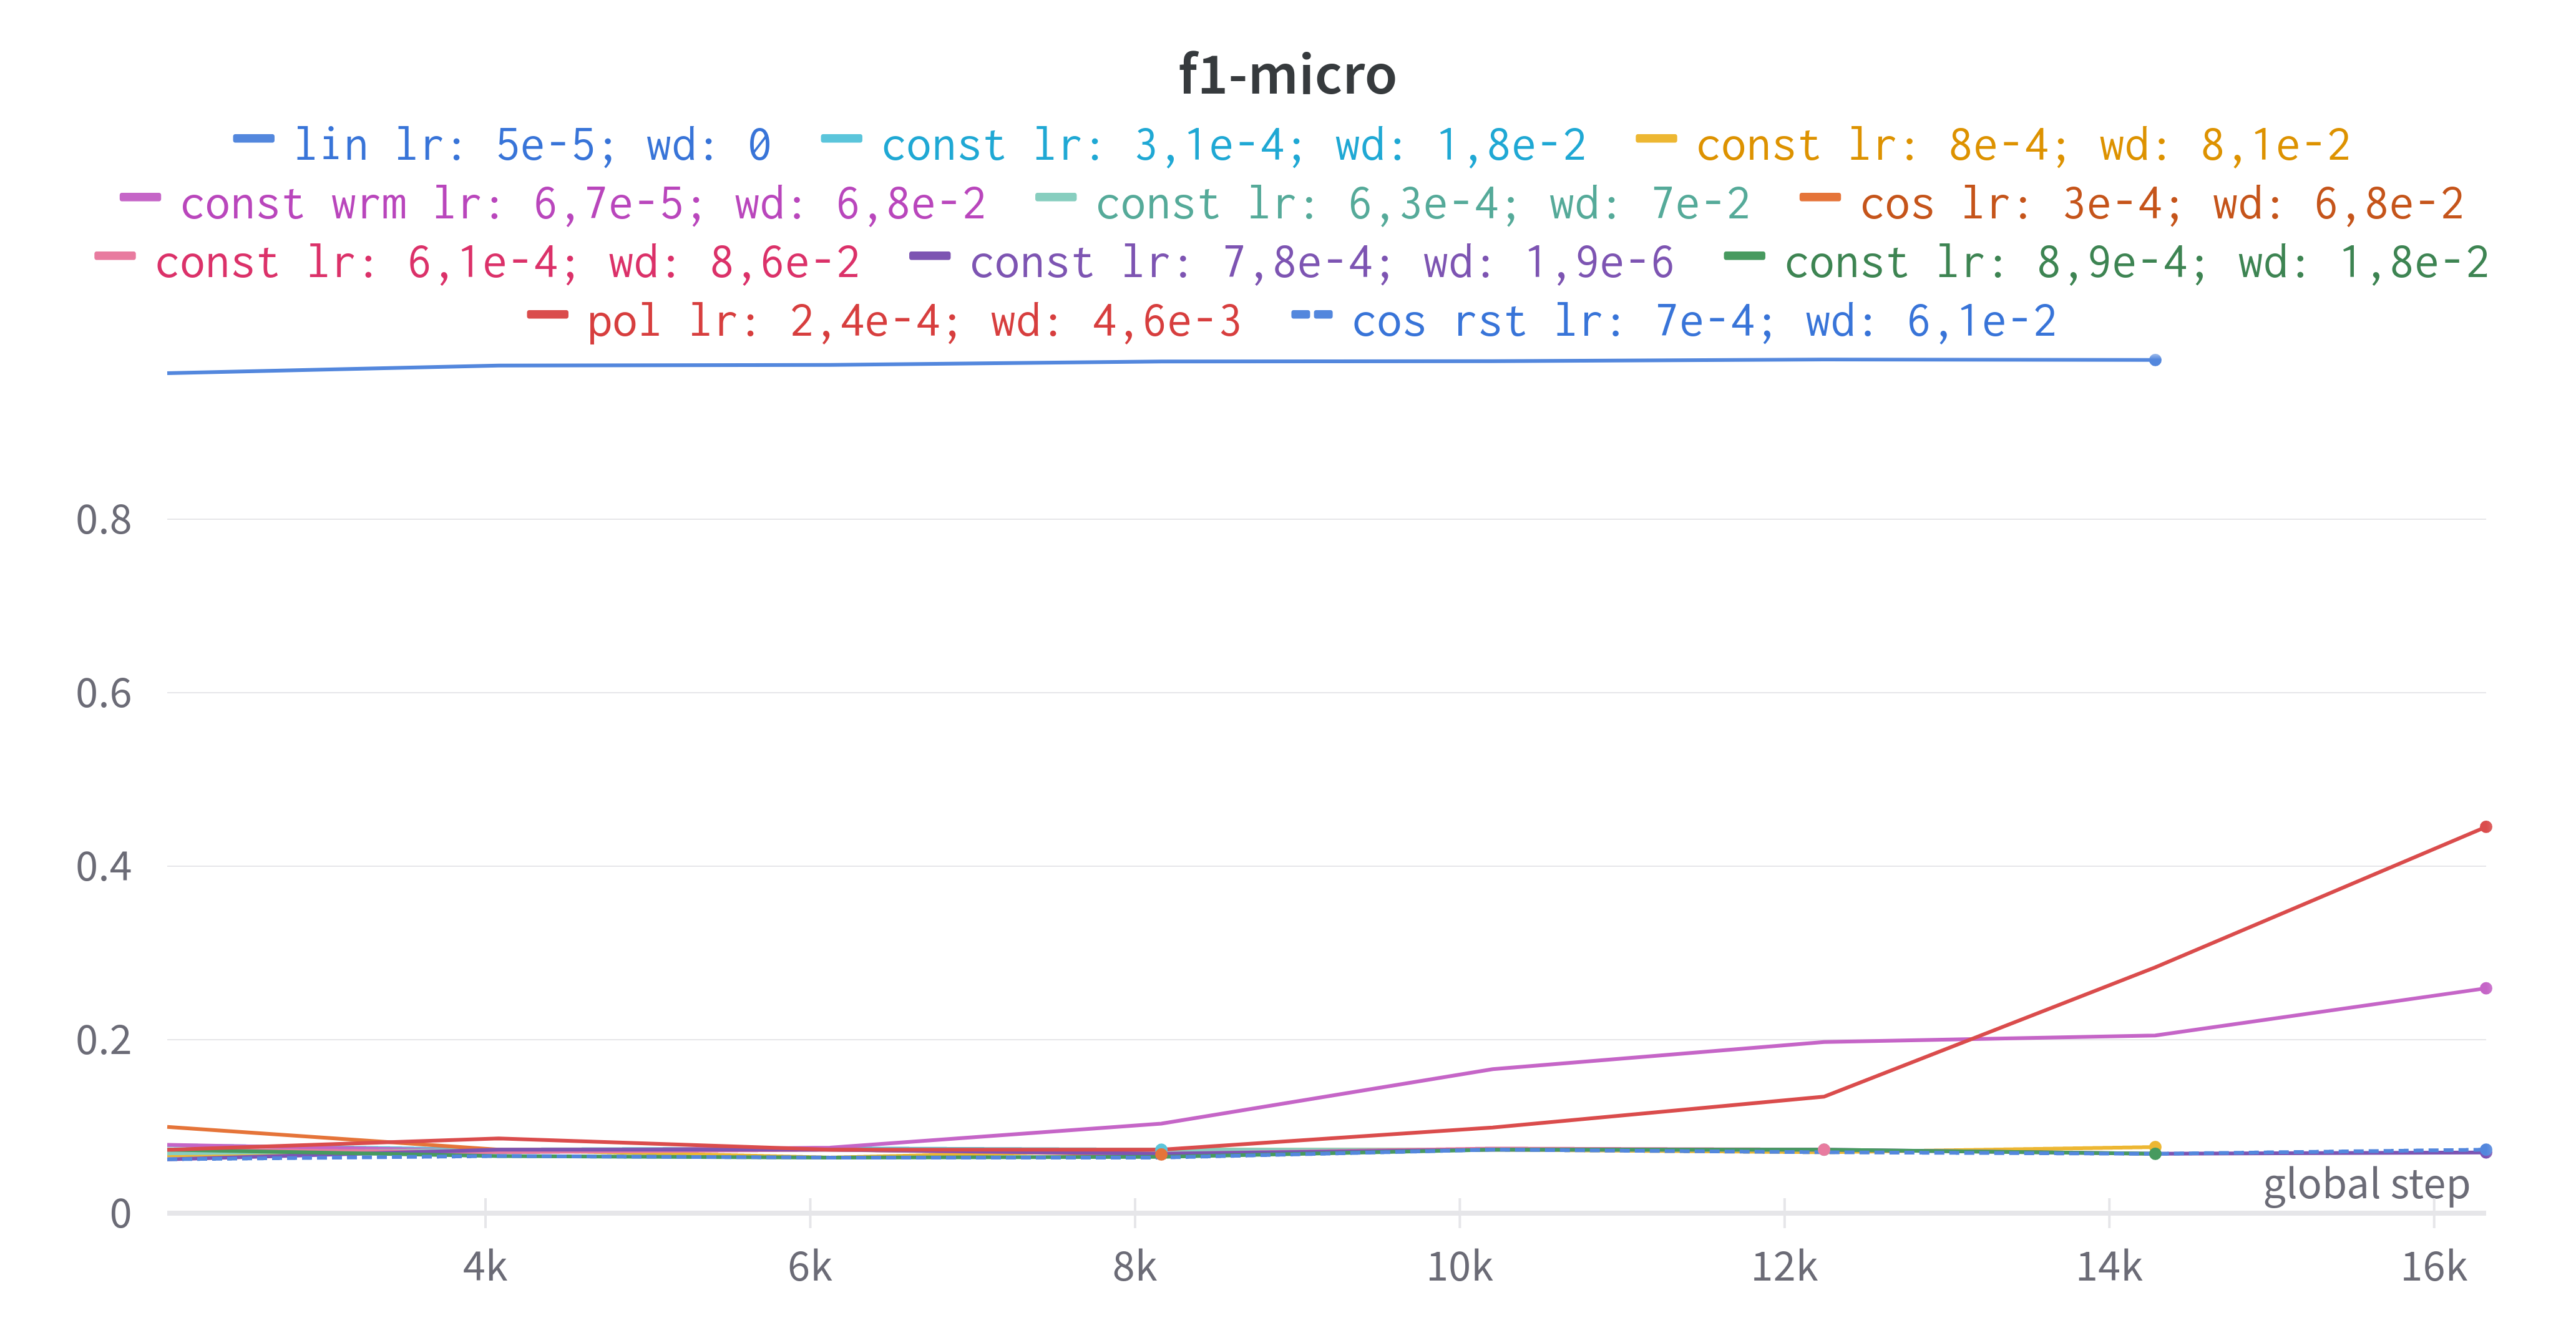
\includegraphics[width=\linewidth]{albert/f1-micro.png}
     \caption{Micro $F_1$ во время обучения ALBERT} 
   \end{minipage}\hfill 
   \begin{minipage}{0.48\textwidth} 
     \centering 
     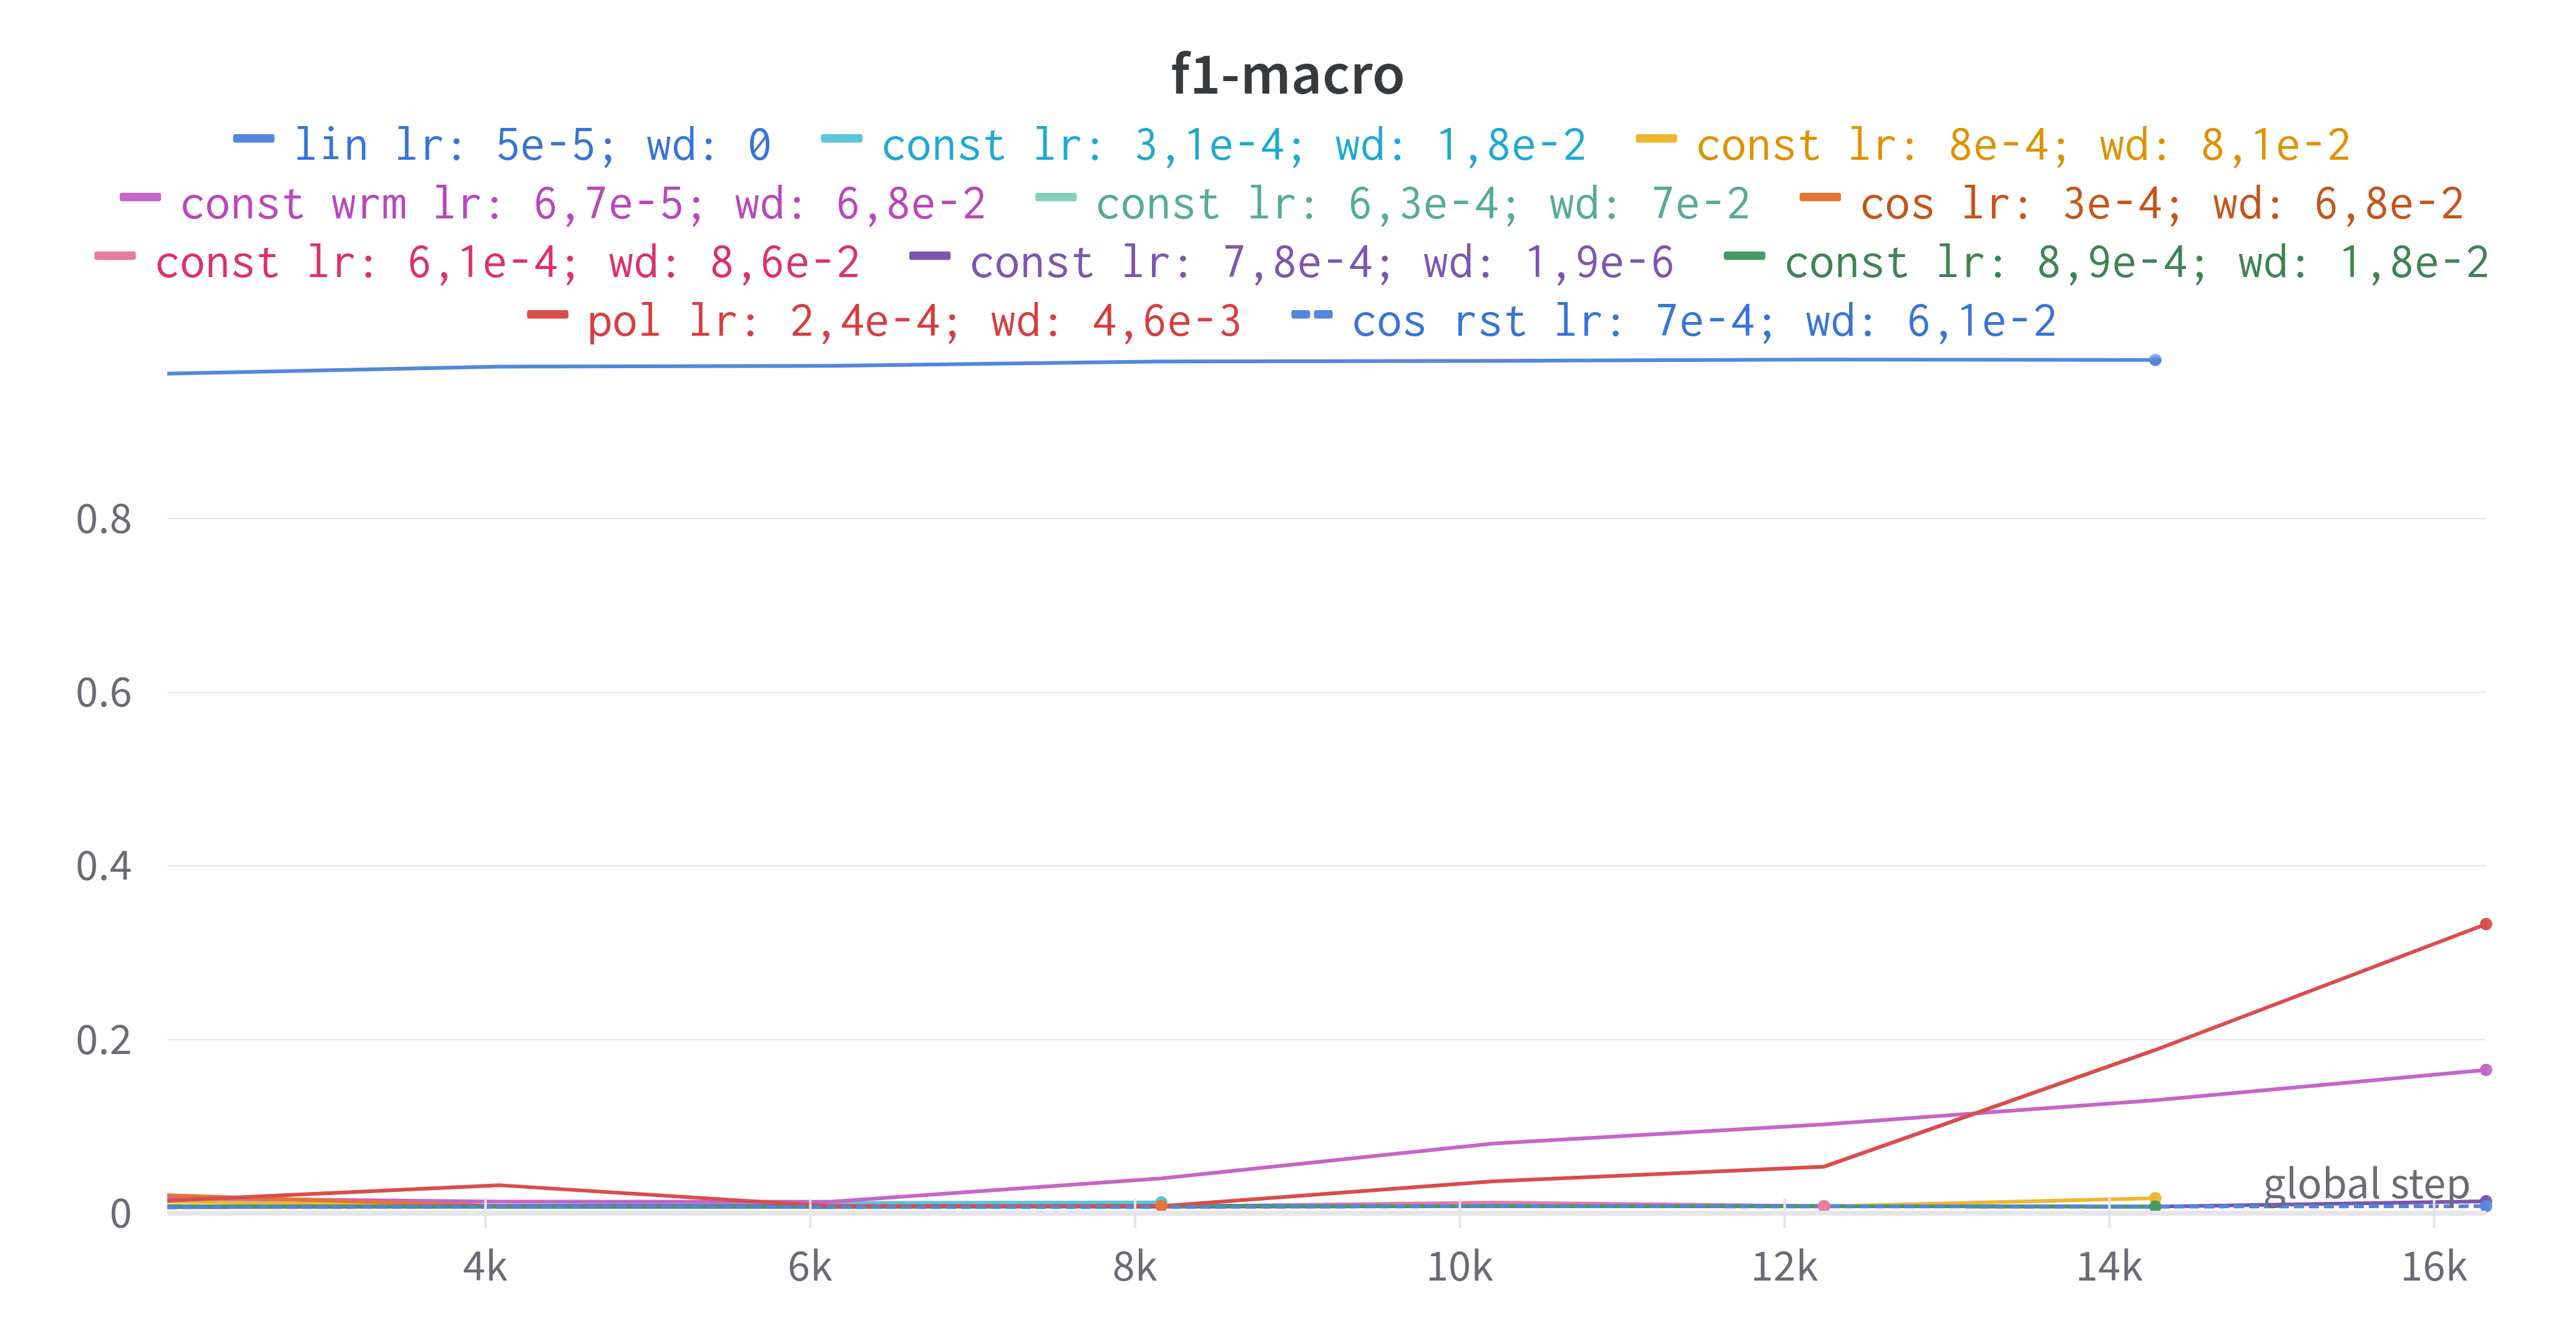
\includegraphics[width=\linewidth]{albert/f1-macro.png}
     \caption{Macro $F_1$ во время обучения ALBERT} 
   \end{minipage} 
\end{figure}

\begin{figure}[!htb] 
   \begin{minipage}{0.48\textwidth} 
     \centering 
     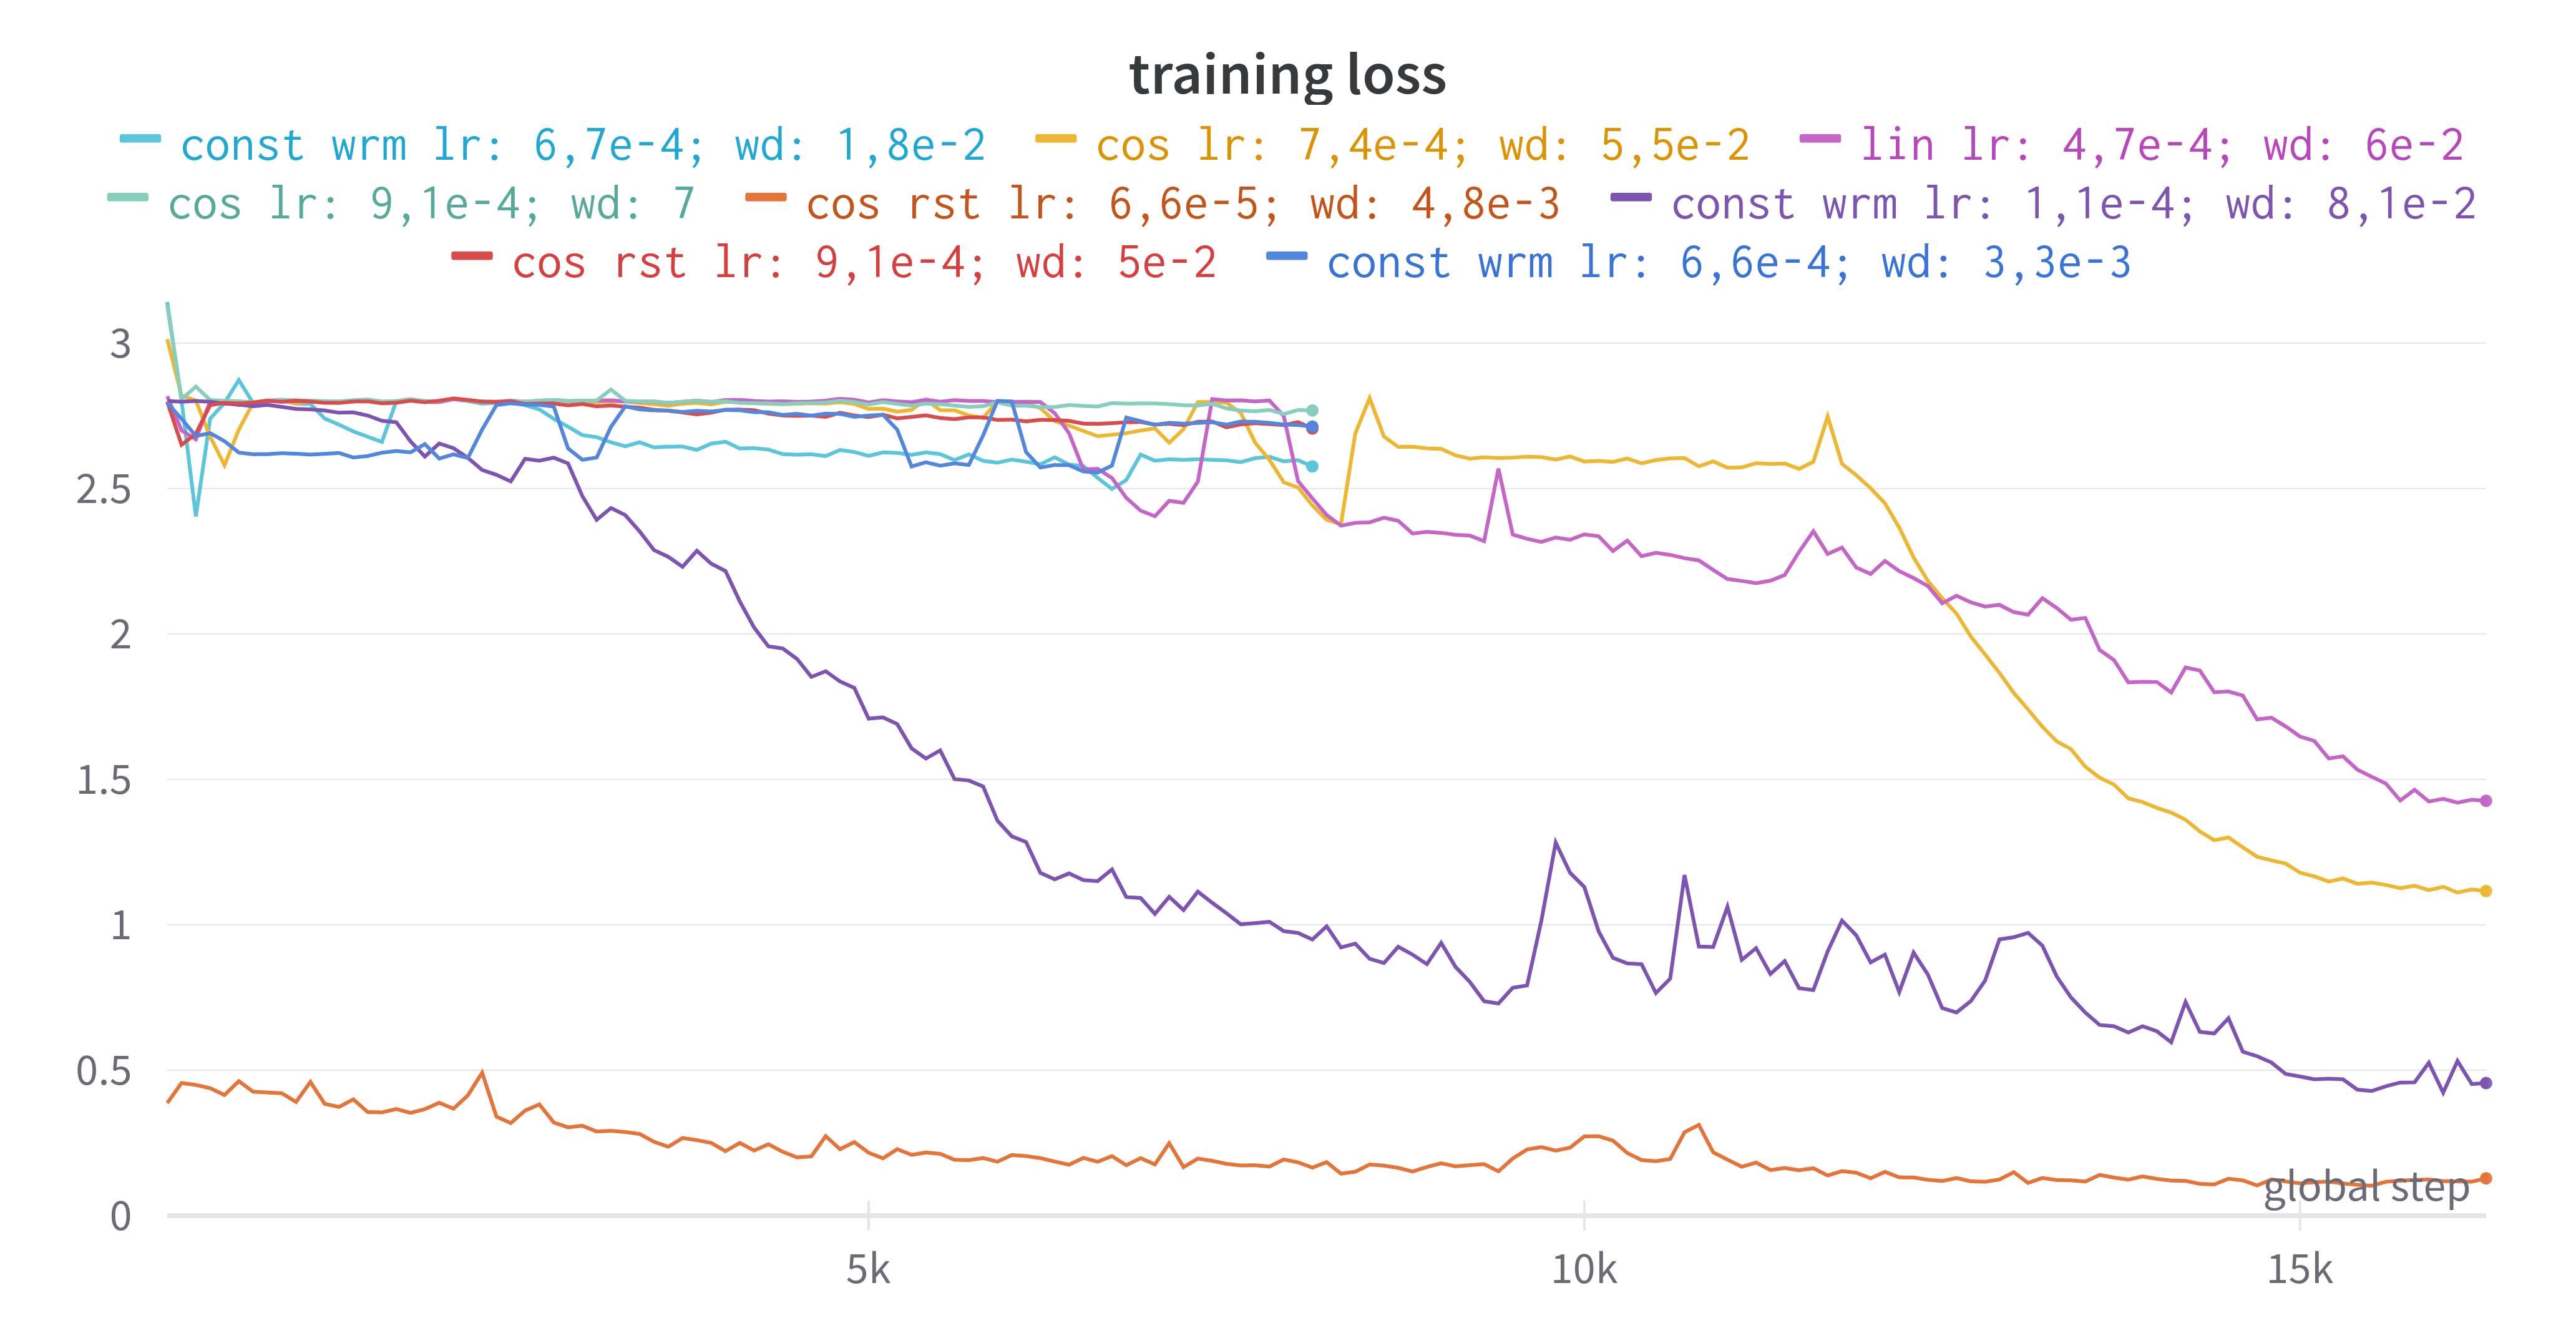
\includegraphics[width=\linewidth]{electra/train-loss.png}
     \caption{График функции ошибки во время обучения ELECTRA} 
   \end{minipage}\hfill 
   \begin{minipage}{0.48\textwidth} 
     \centering 
     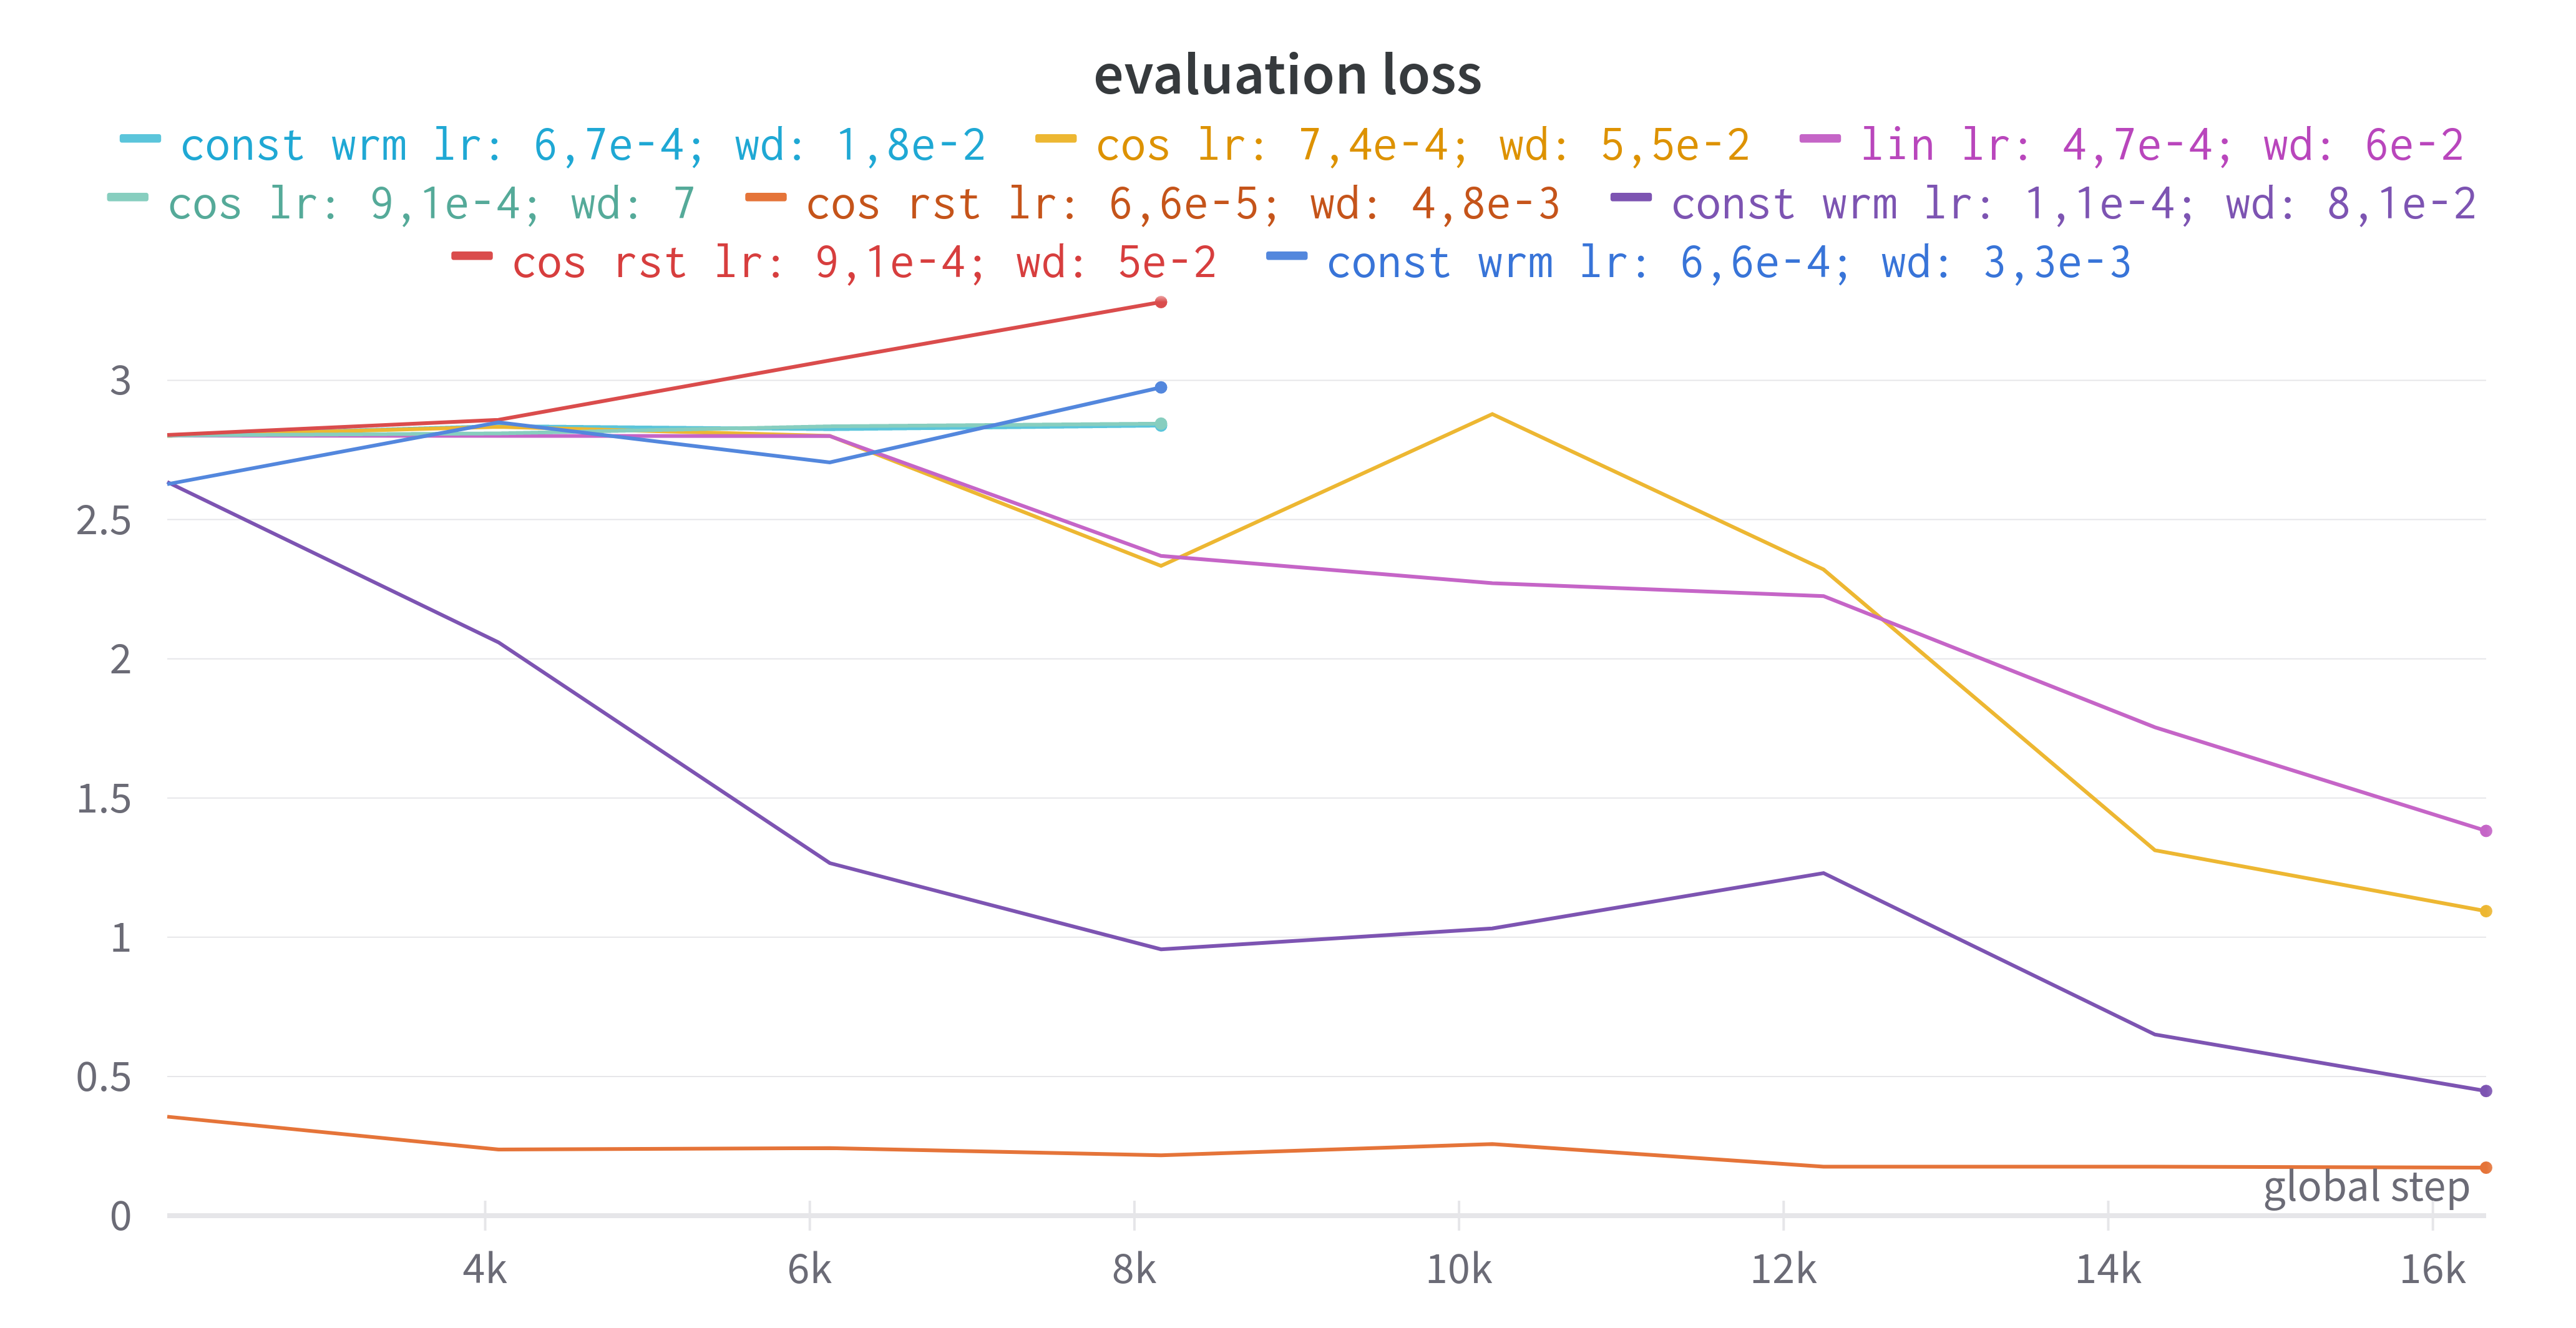
\includegraphics[width=\linewidth]{electra/eval-loss.png}
     \caption{График функции ошибки при валидации ELECTRA} 
   \end{minipage} 
\end{figure}

\begin{figure}[!htb] 
   \begin{minipage}{0.48\textwidth} 
     \centering 
     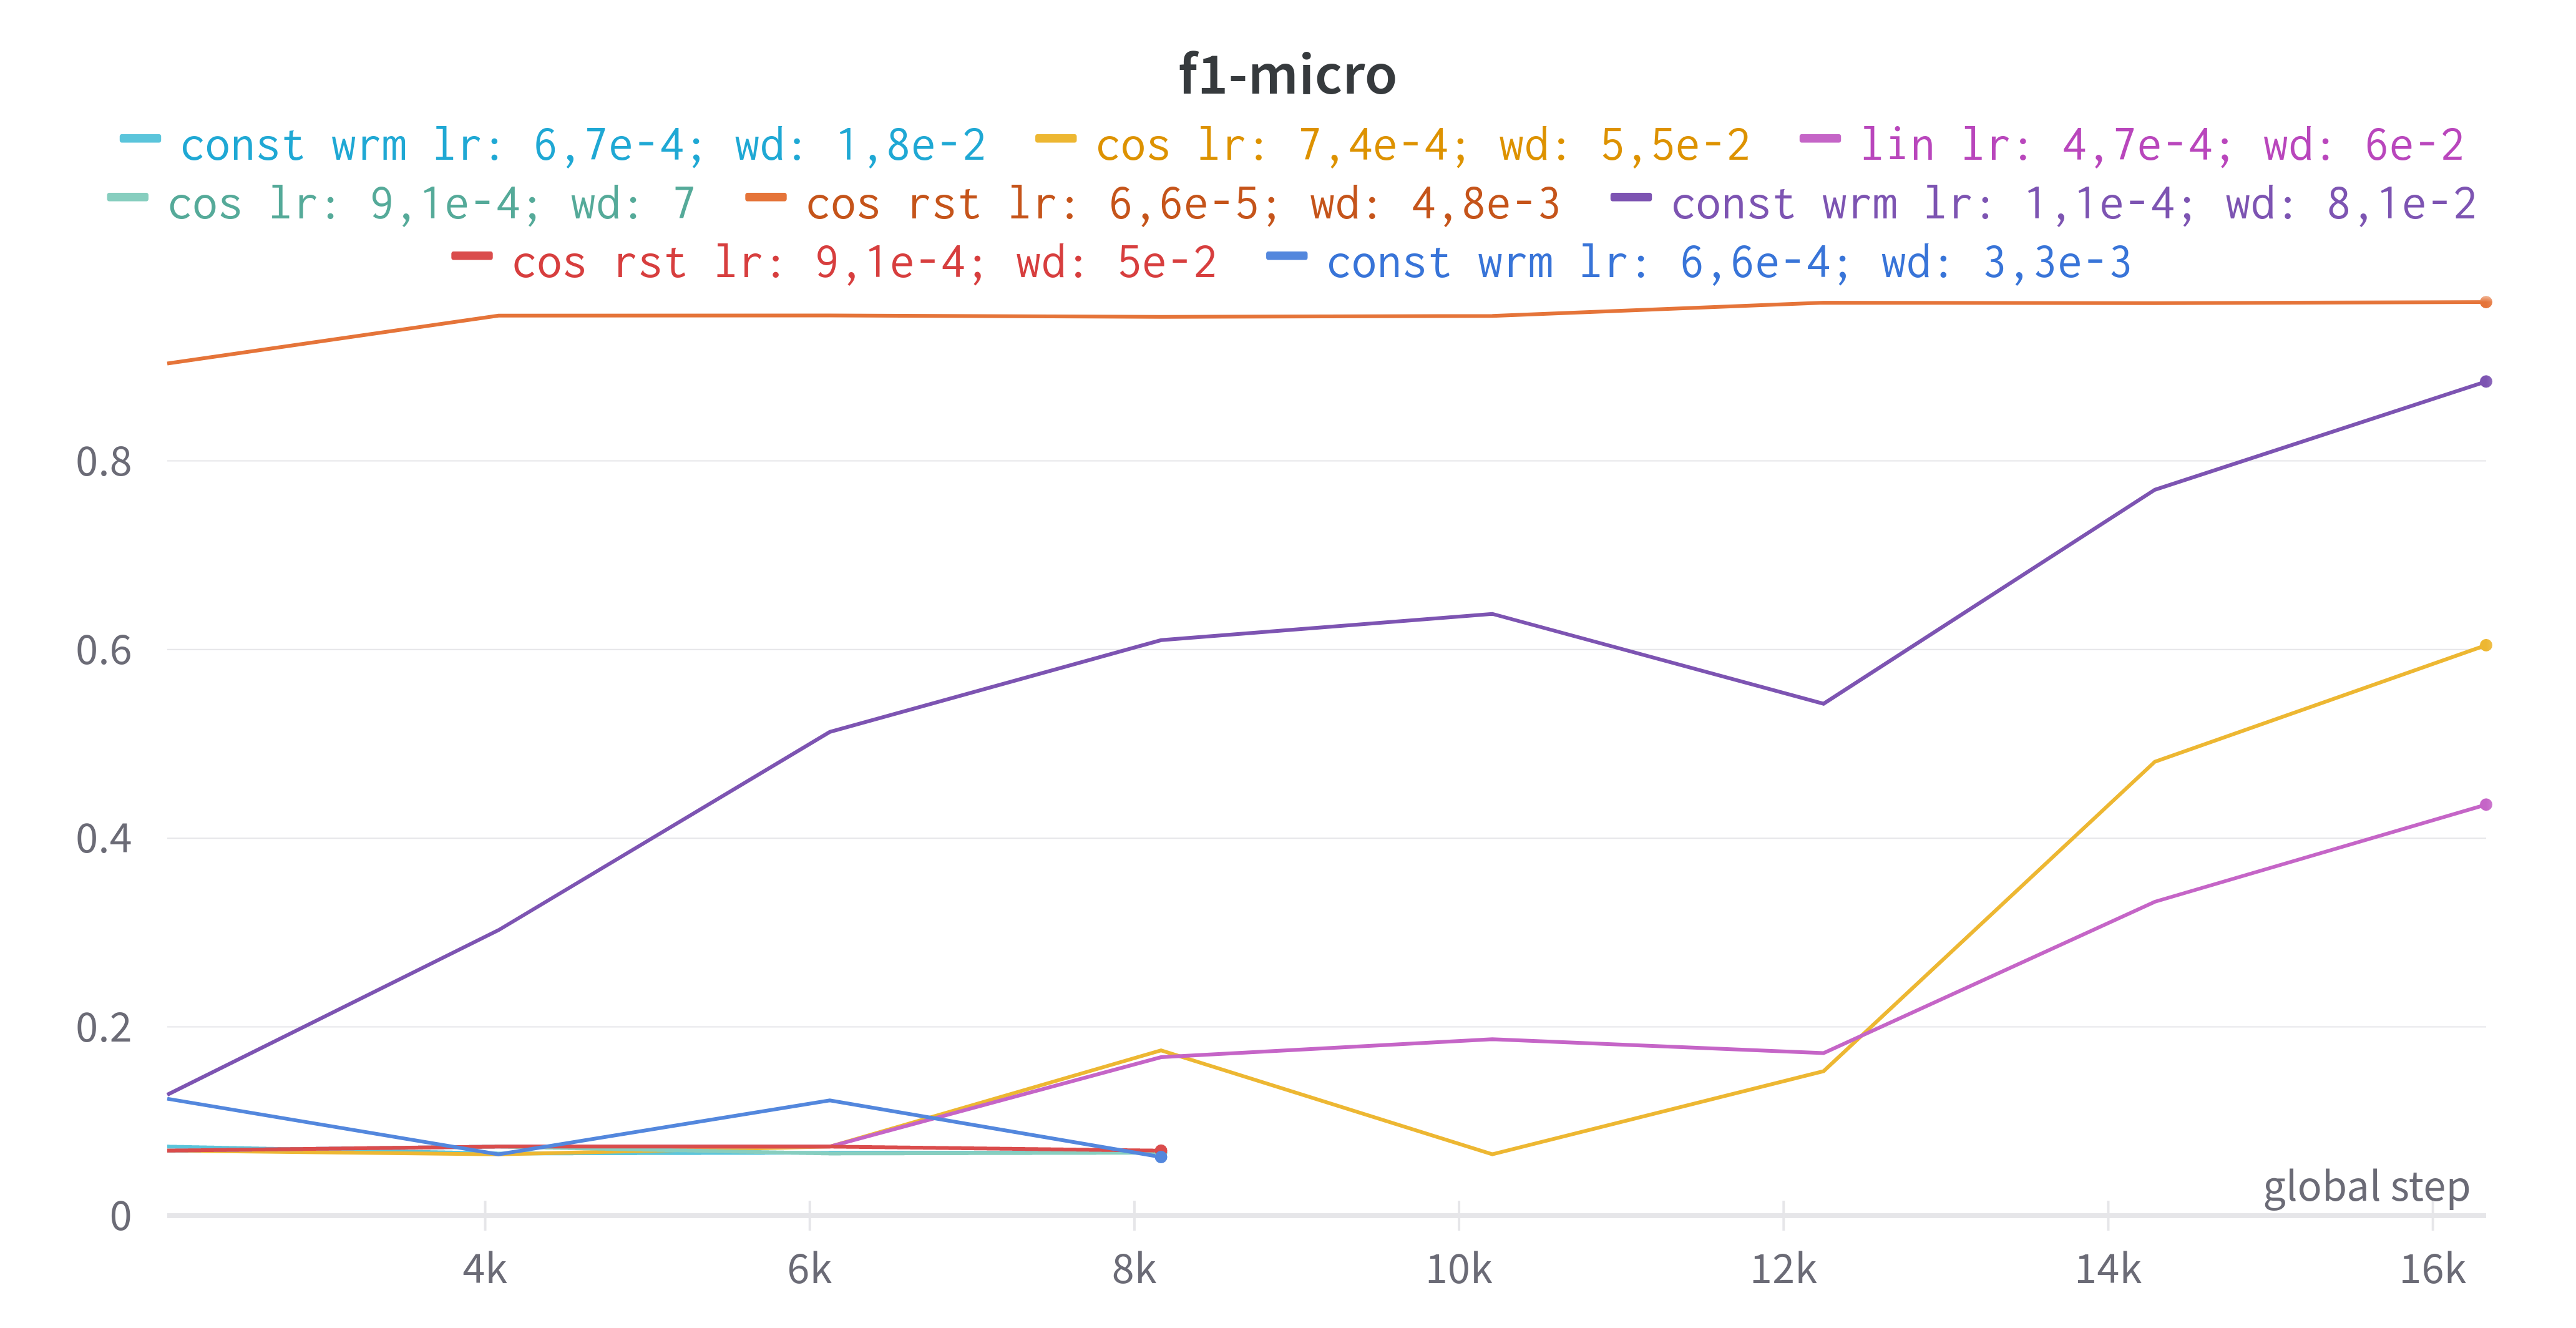
\includegraphics[width=\linewidth]{electra/f1-micro.png}
     \caption{Micro $F_1$ во время обучения ELECTRA} 
   \end{minipage}\hfill 
   \begin{minipage}{0.48\textwidth} 
     \centering 
     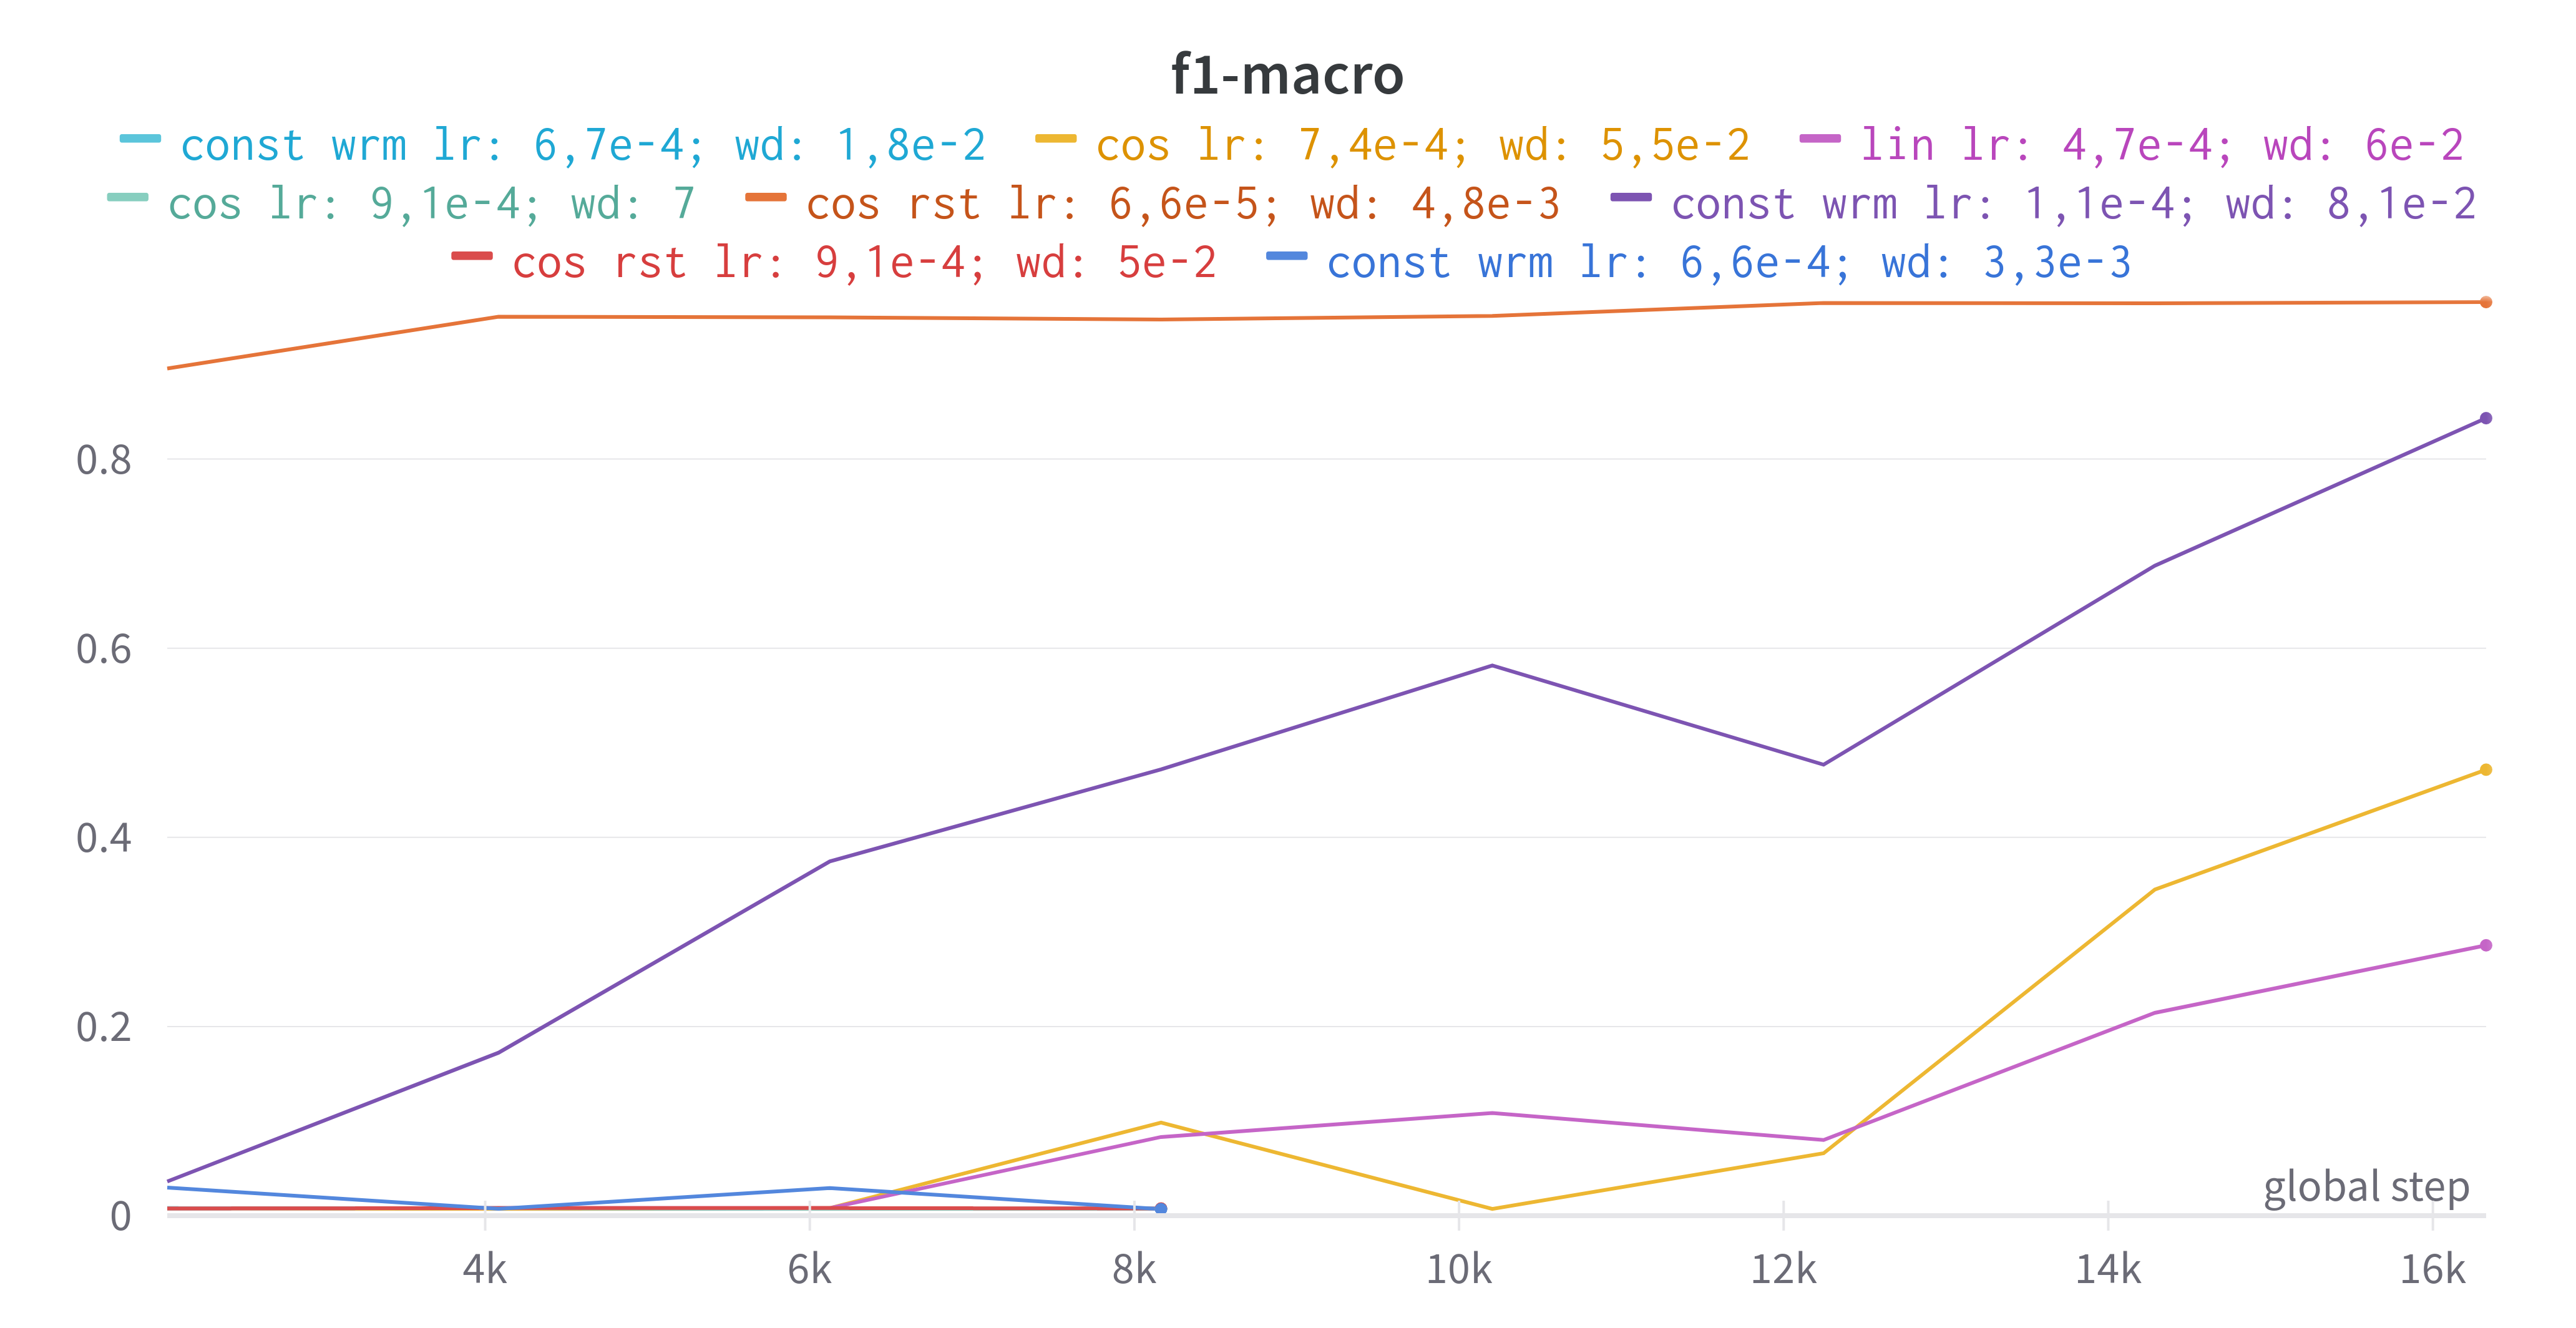
\includegraphics[width=\linewidth]{electra/f1-macro.png}
     \caption{Macro $F_1$ во время обучения ELECTRA} 
   \end{minipage} 
\end{figure}

\begin{figure}[!htb] 
   \begin{minipage}{0.48\textwidth} 
     \centering 
     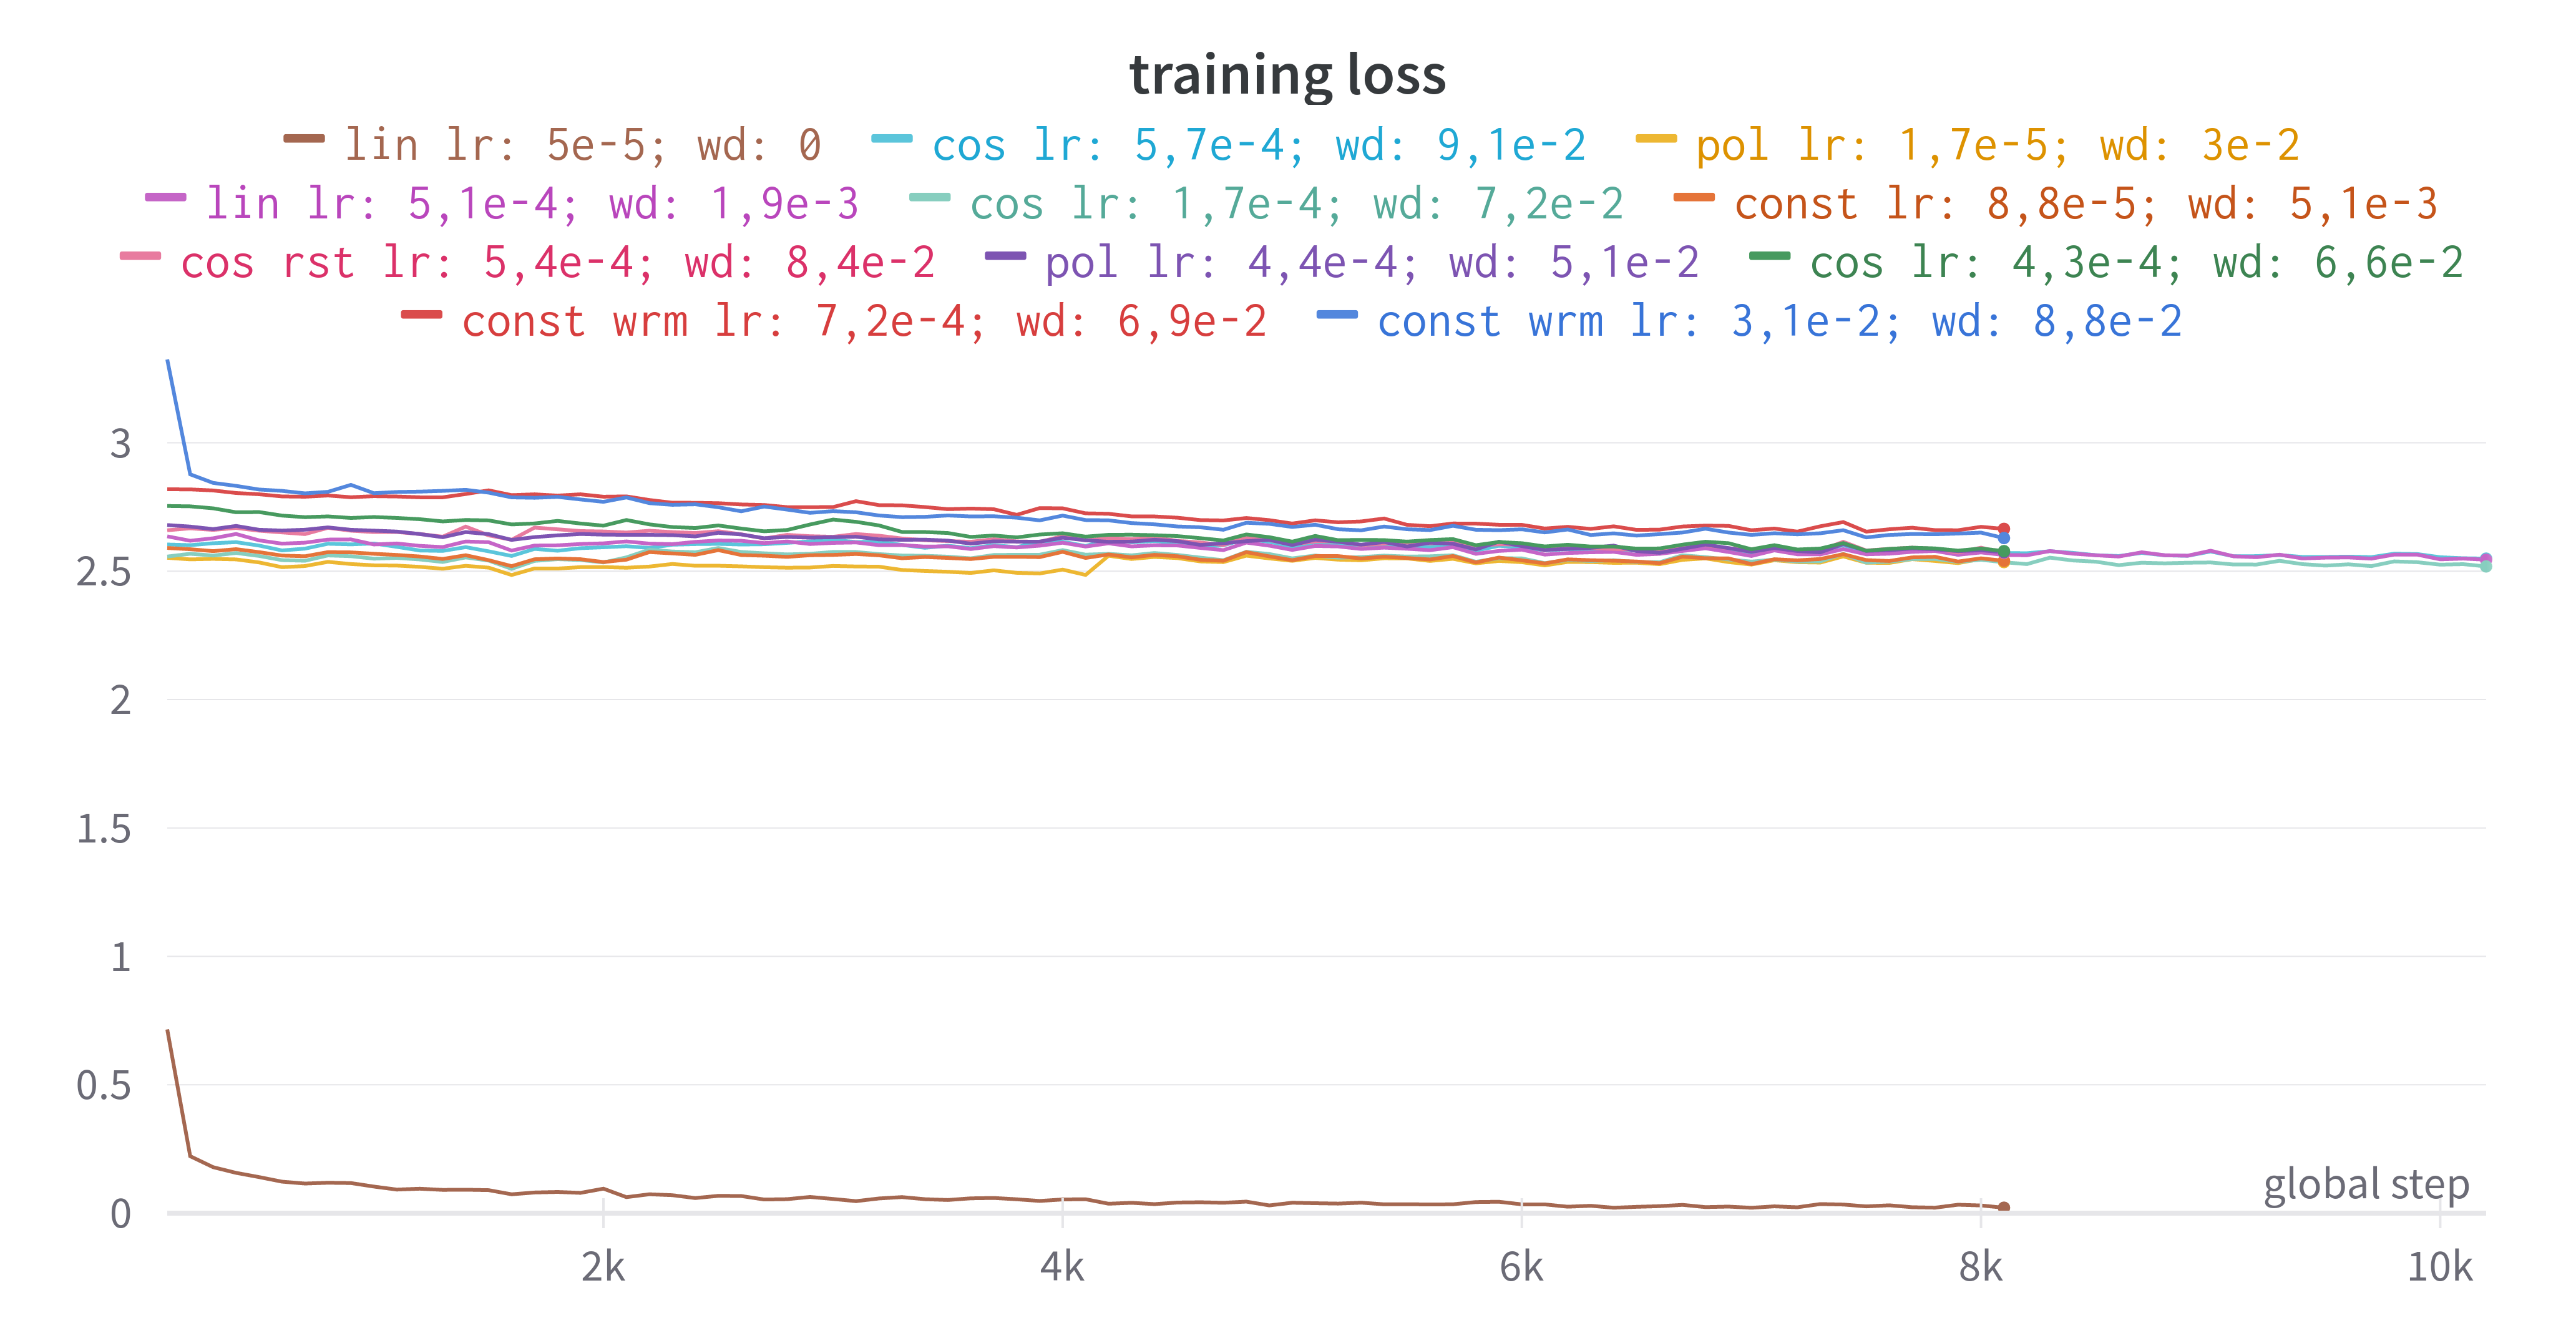
\includegraphics[width=\linewidth]{opt/train-loss.png}
     \caption{График функции ошибки во время обучения OPT} 
   \end{minipage}\hfill 
   \begin{minipage}{0.48\textwidth} 
     \centering 
     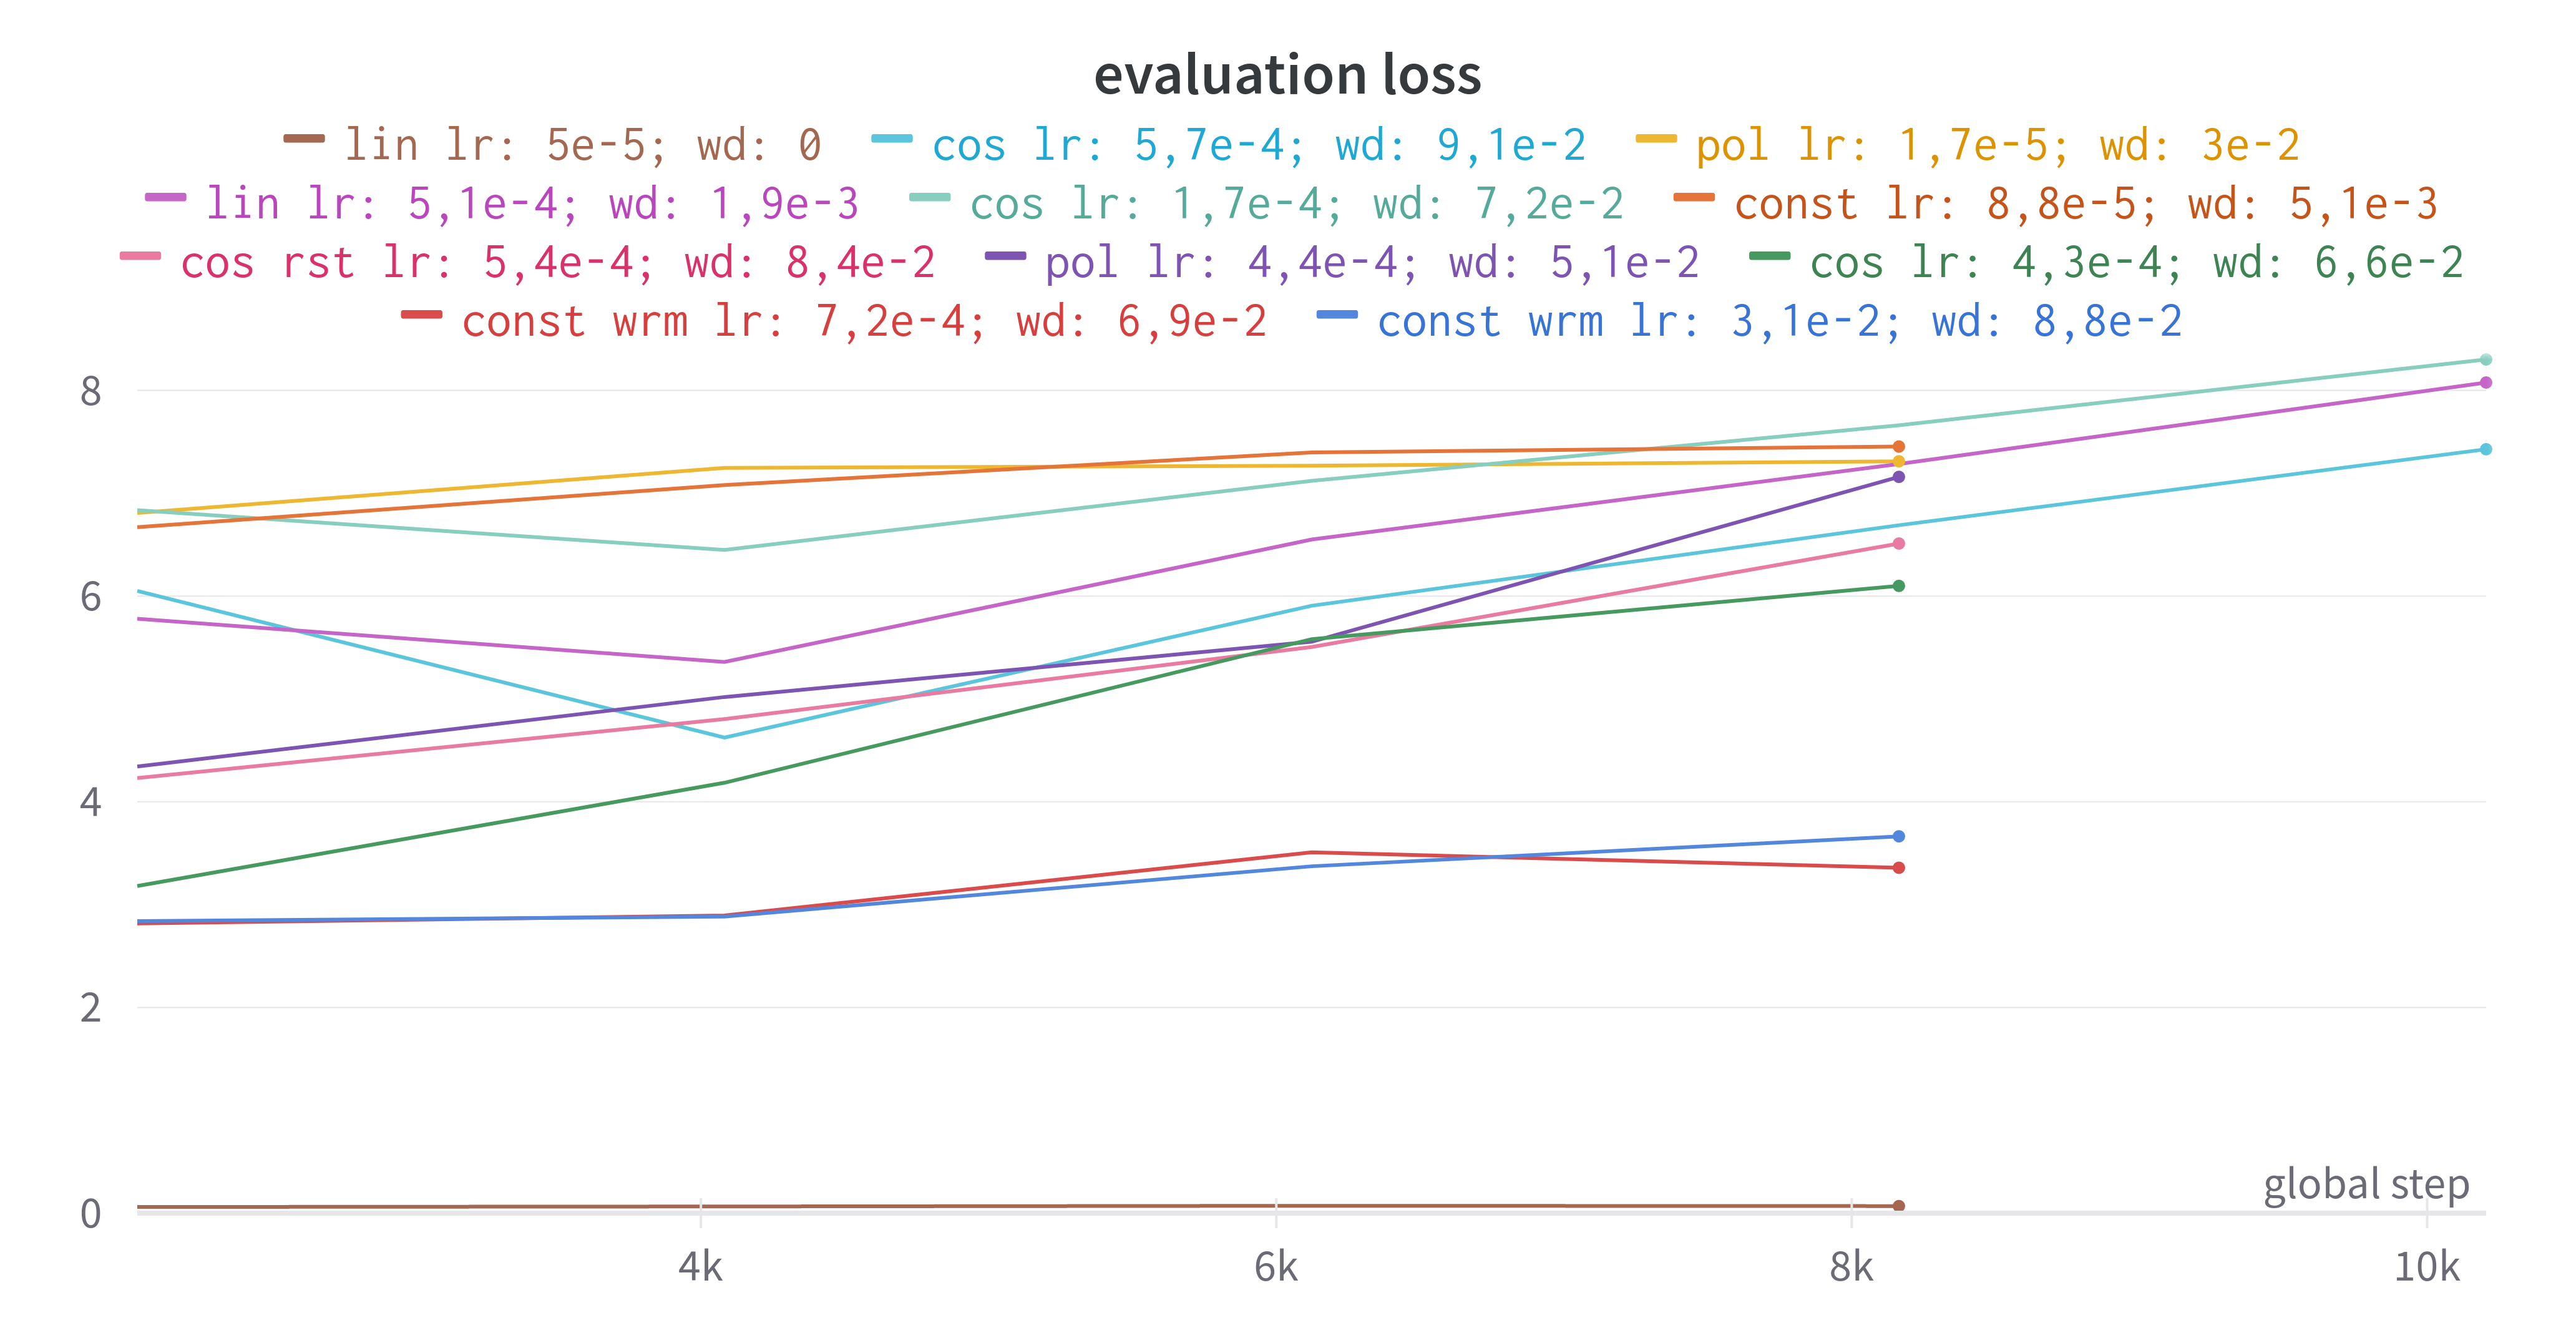
\includegraphics[width=\linewidth]{opt/eval-loss.png}
     \caption{График функции ошибки при валидации OPT} 
   \end{minipage} 
\end{figure}

\begin{figure}[!htb] 
   \begin{minipage}{0.48\textwidth} 
     \centering 
     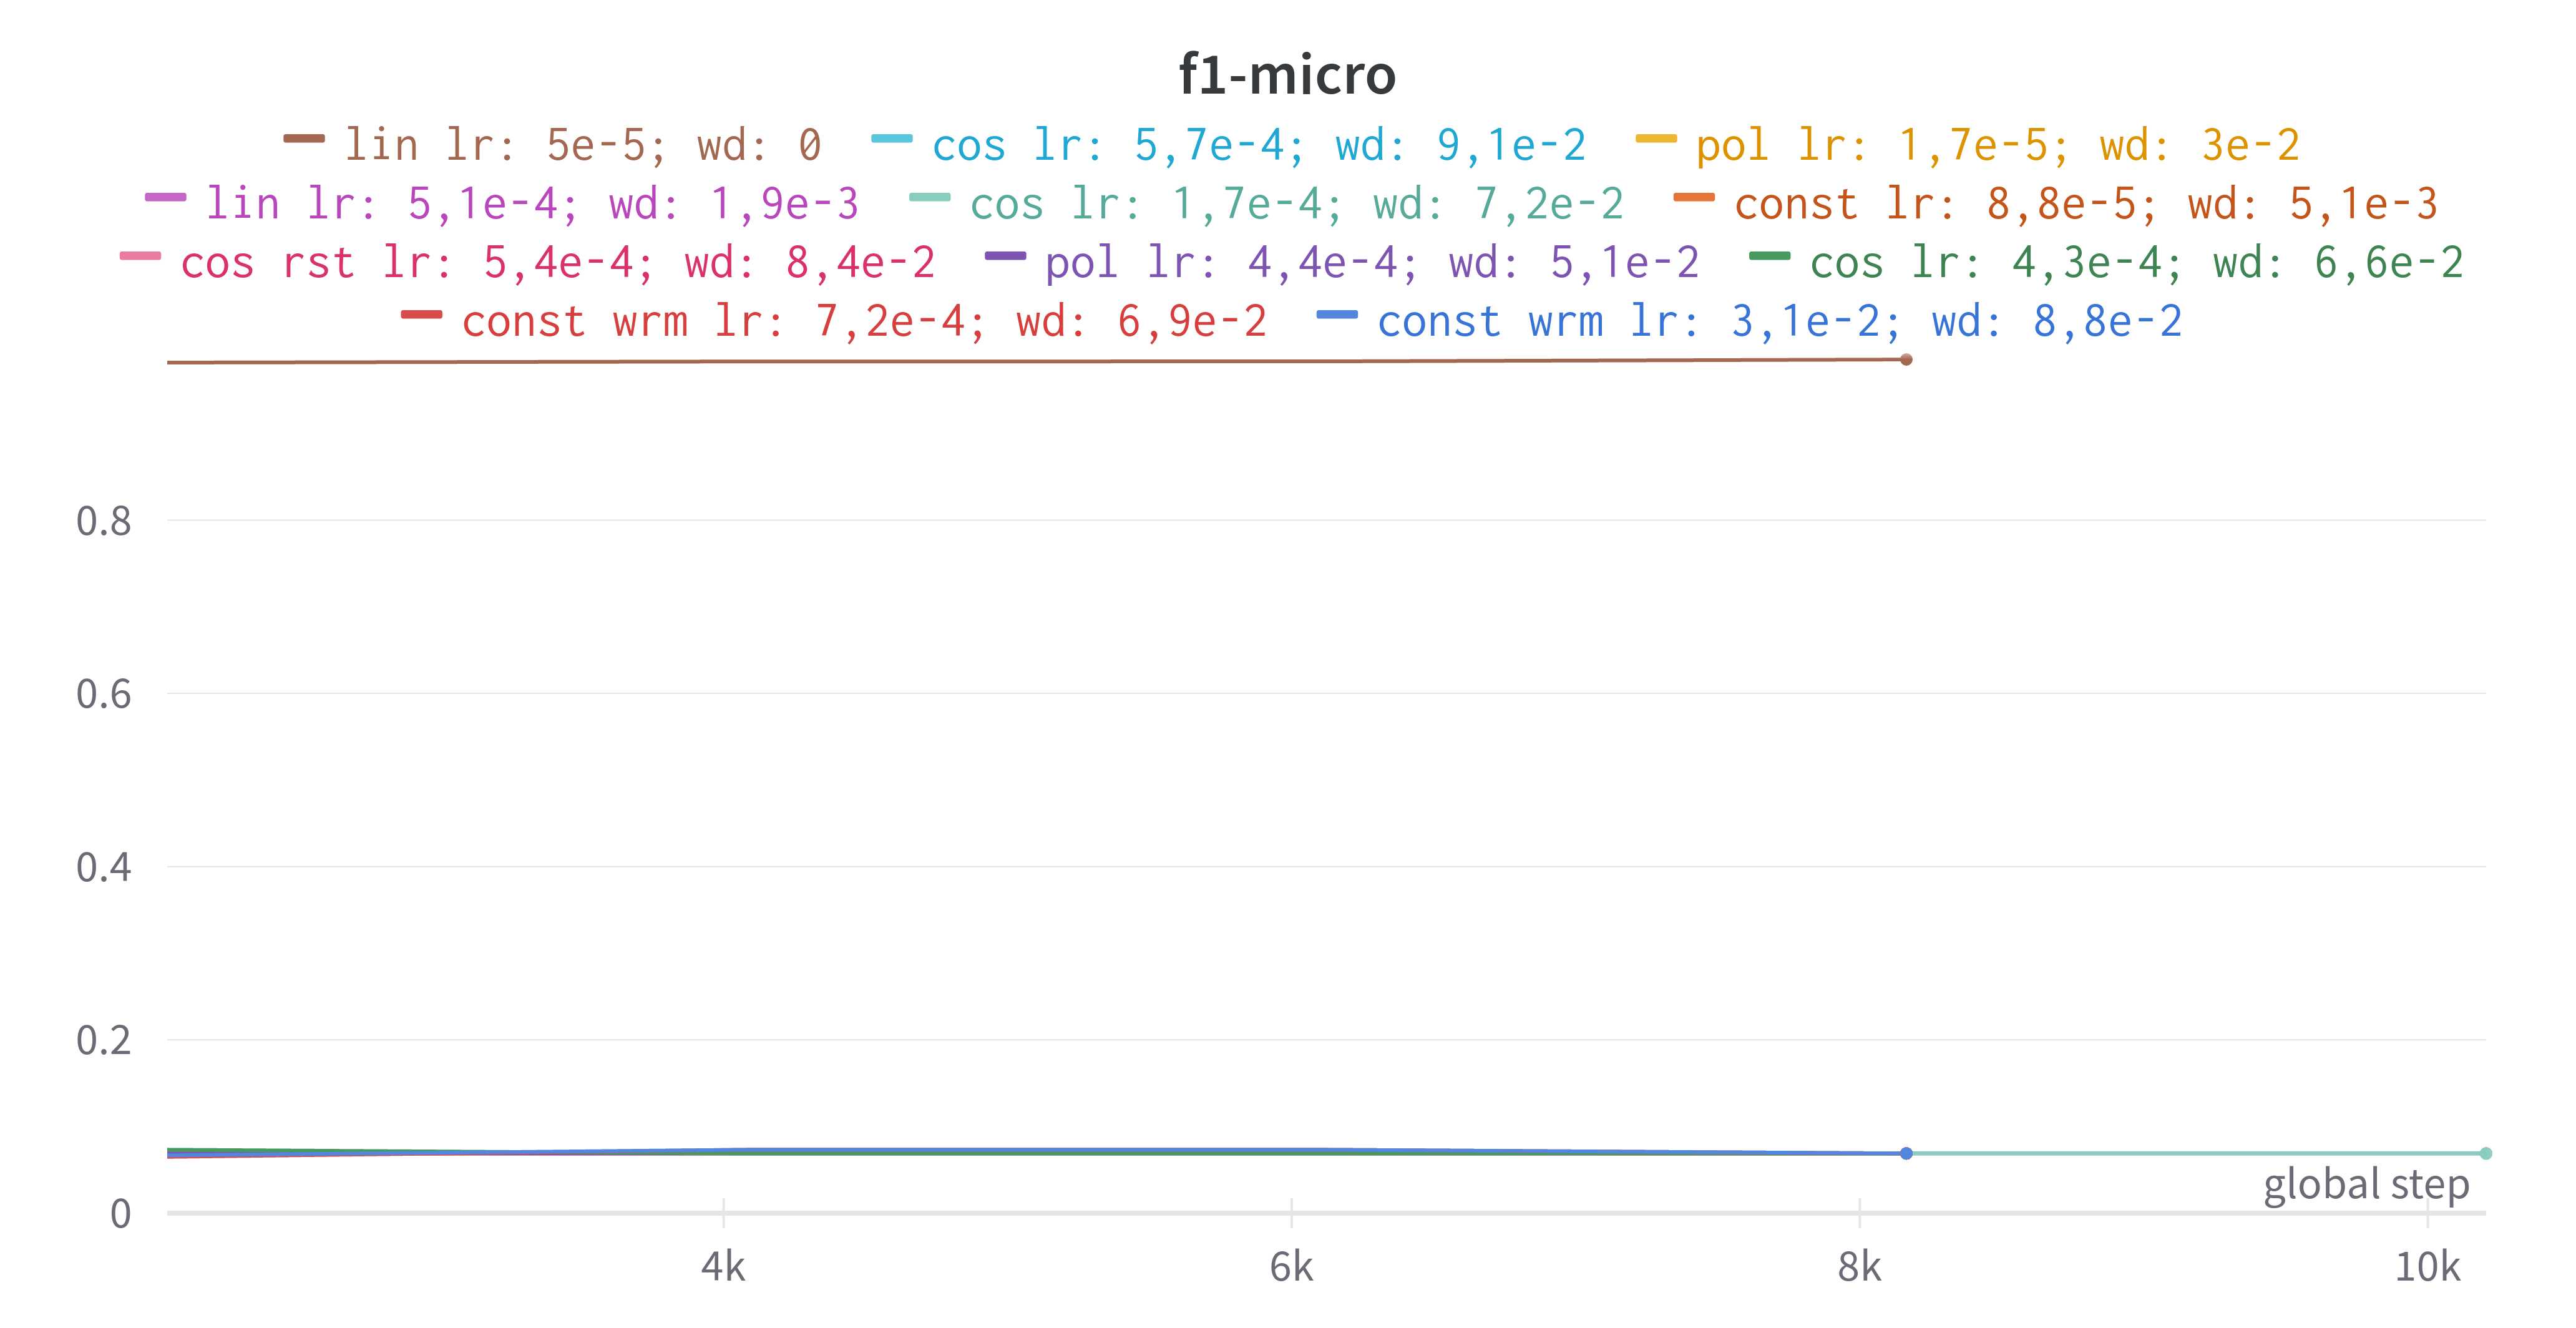
\includegraphics[width=\linewidth]{opt/f1-micro.png}
     \caption{Micro $F_1$ во время обучения OPT} 
   \end{minipage}\hfill 
   \begin{minipage}{0.48\textwidth} 
     \centering 
     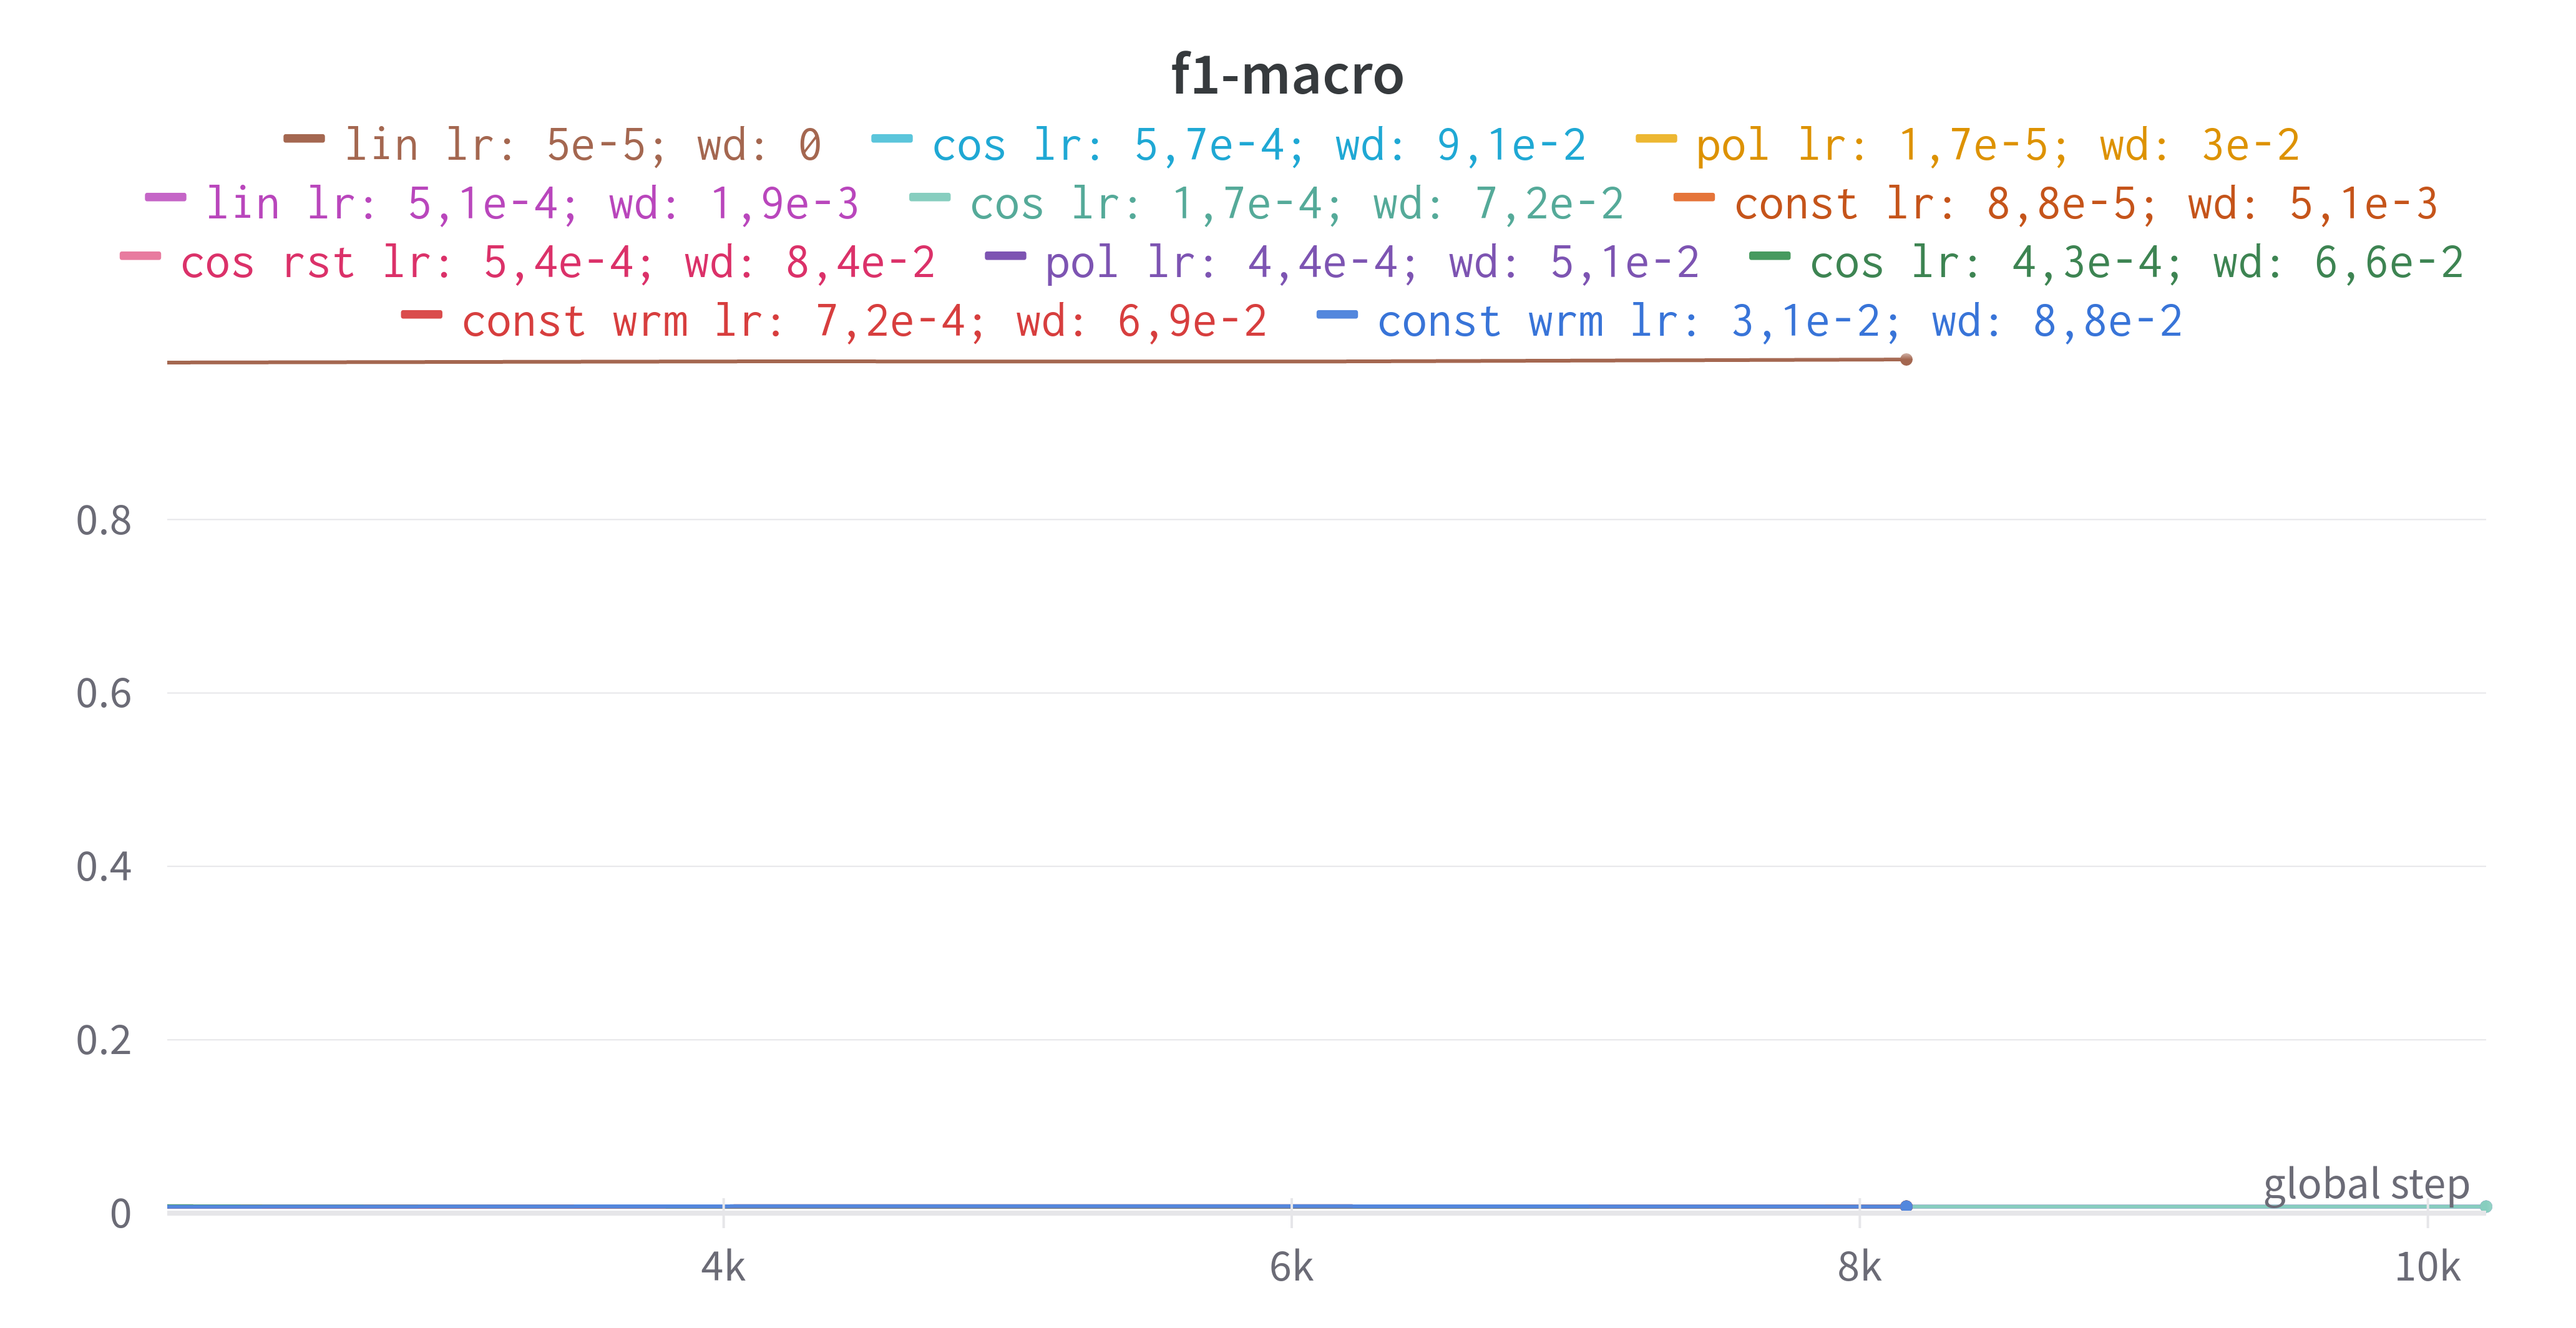
\includegraphics[width=\linewidth]{opt/f1-macro.png}
     \caption{Macro $F_1$ во время обучения OPT} 
   \end{minipage} 
\end{figure}
\chapter{ГРАФИКИ ПРИ ОБУЧЕНИИ МОДЕЛЕЙ ДЛЯ СРАВНЕНИЯ}
  \label{app:models}\begin{figure}[!htb] 
   \centering 
   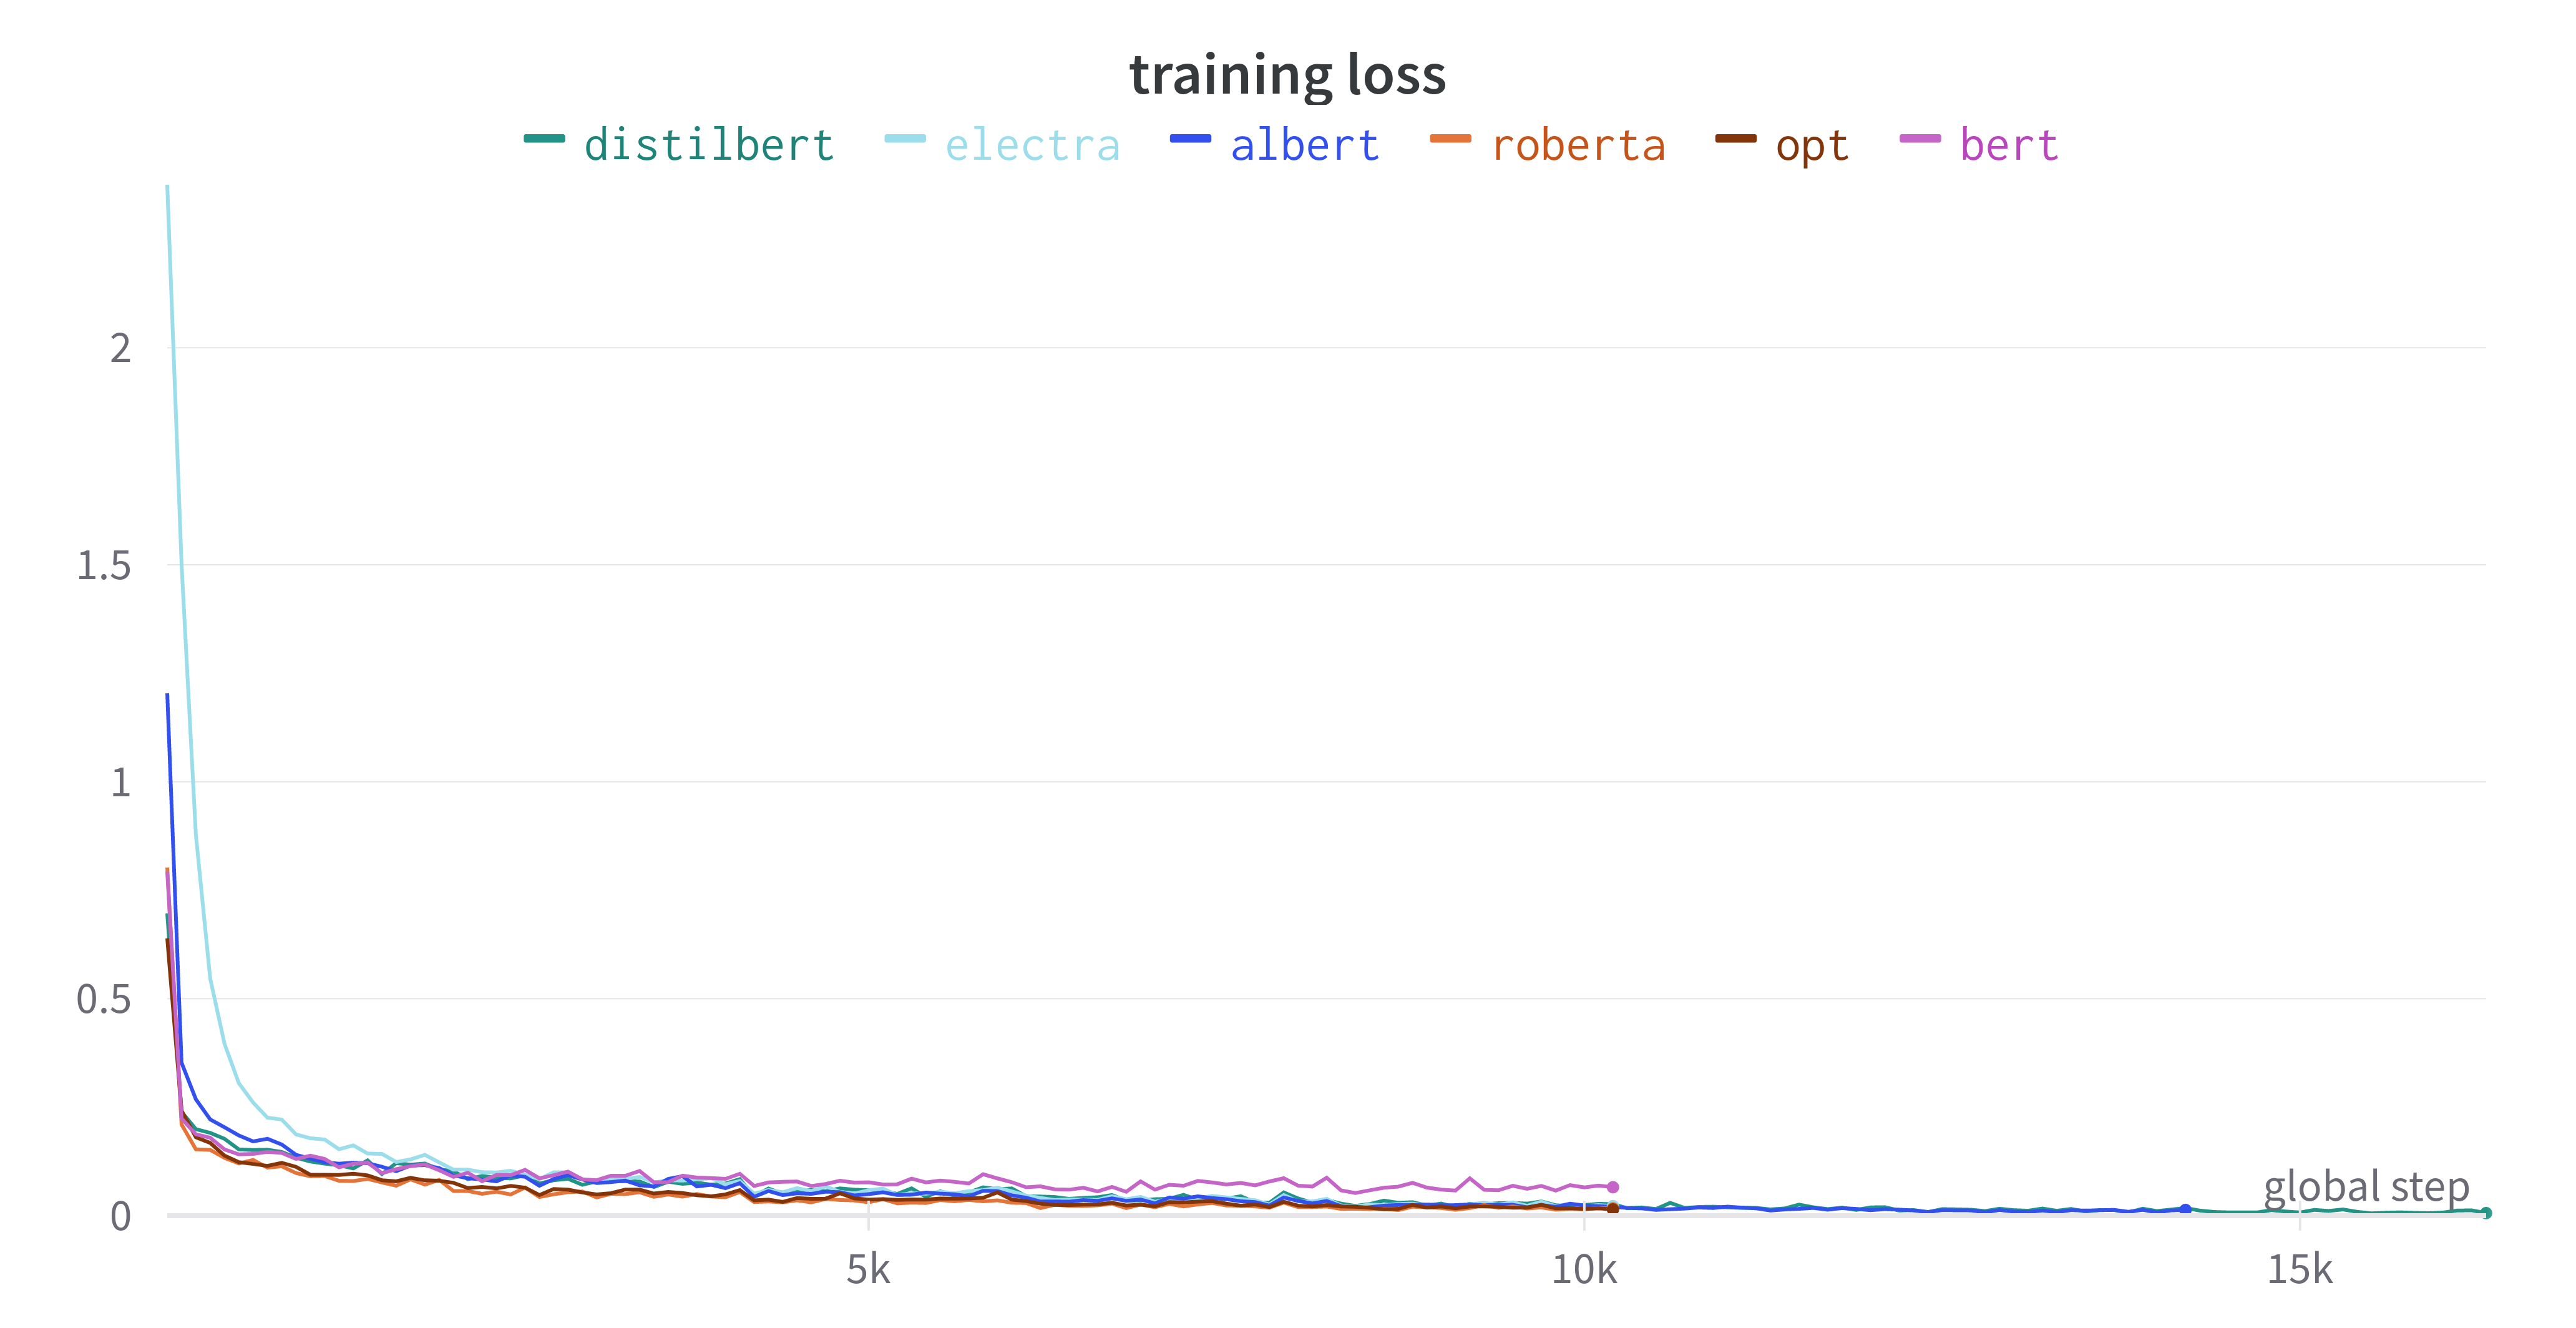
\includegraphics[width=0.9\linewidth]{models/train-loss.png}
   \caption{График функции ошибки во время обучения моделей} 
\end{figure} 

\begin{figure}[!htb] 
   \centering 
   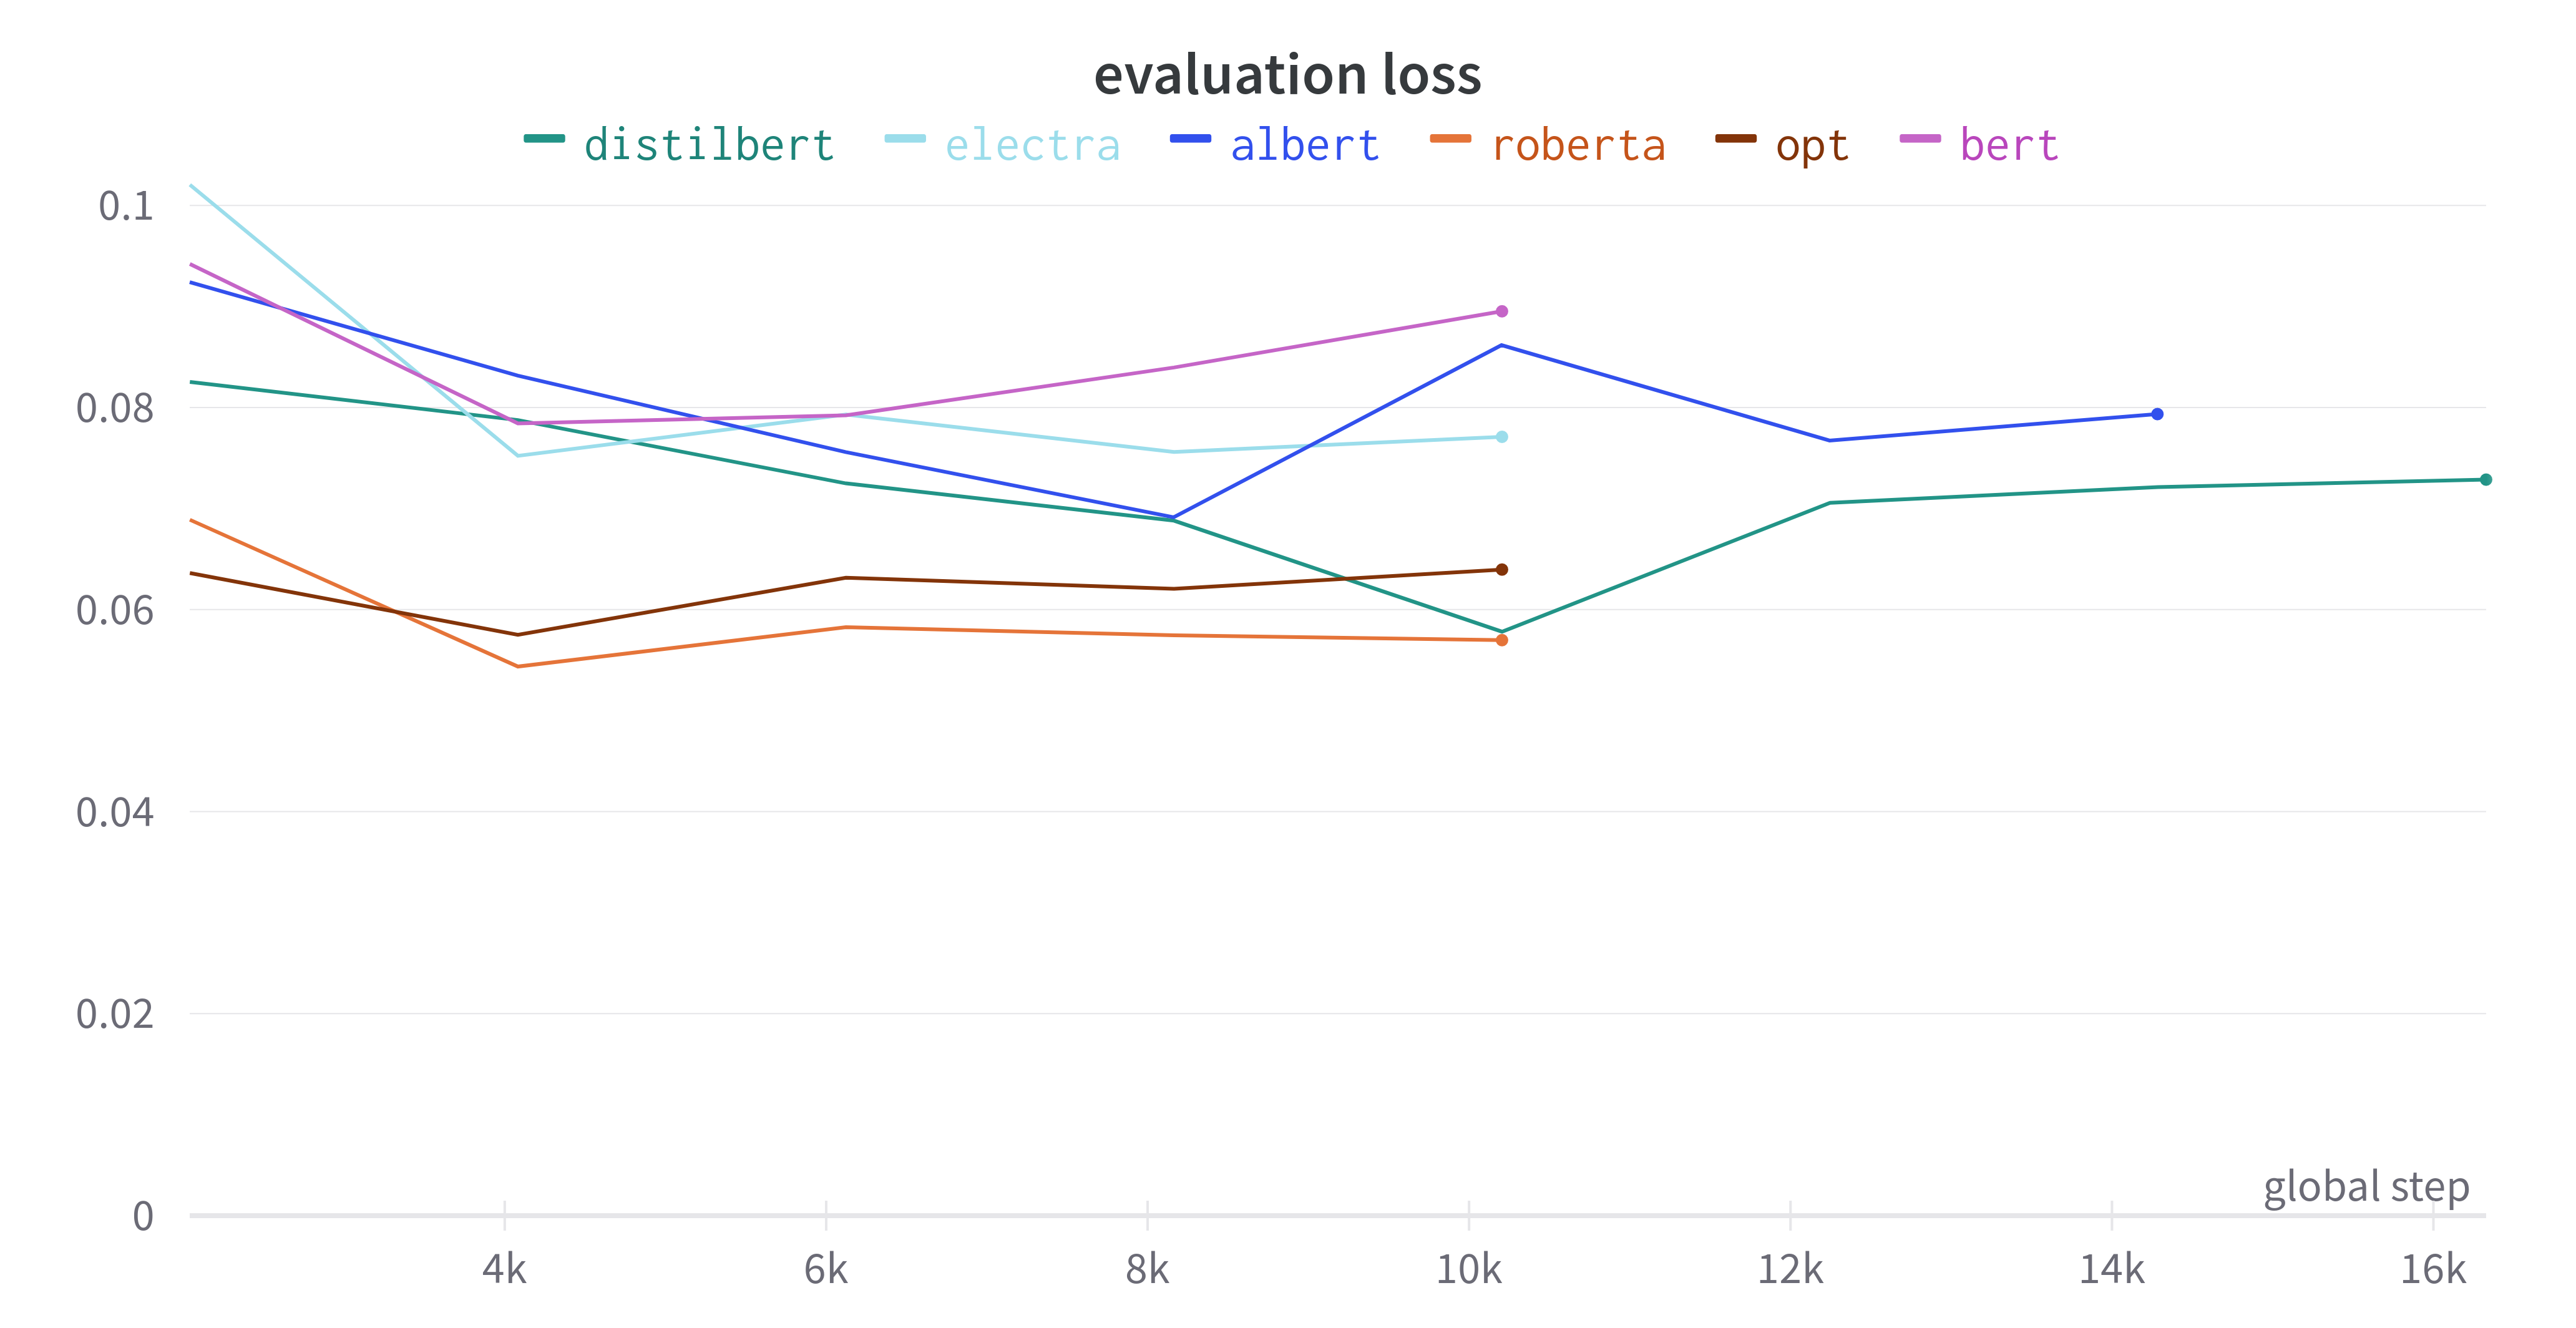
\includegraphics[width=0.9\linewidth]{models/eval-loss.png}
   \caption{График функции ошибки при валидации моделей} 
\end{figure} 
\end{document}